\documentclass[a4paper,12pt]{article}
\usepackage[a4paper,left=2cm,right=2cm]{geometry}
\usepackage[english]{babel}
\usepackage[latin1]{inputenc}
\usepackage{graphicx}
\usepackage[formats]{listings}
\usepackage{fancyvrb}
\usepackage{multicol}
\usepackage{mdframed}
\usepackage{subfig}
\usepackage{upquote}
\usepackage[font=footnotesize]{caption}
\usepackage{hyperref}


\begin{document}
\title{IN480 \hspace{0.5cm} Larstruct Module}
\author{Desiree Adiutori \and Alessia Giulia Cossu}
\maketitle
\tableofcontents
\listoffigures
\newpage
\section*{Introduction}
\addcontentsline{toc}{section}{Introduction}
This module of LAR-CC library deals with the hierarchical structures with LAR. Hierarchical
models of complex assemblies are generated by an aggregation of subassemblies, each one defined
in a local coordinates’ system, and relocated by affine transformations of coordinates.

In this module there are:
\begin{itemize}
\item The \textbf{Affine transformations} whom are based on elementary matrices for affine trans-
formations of vectors in any dimensional vector space, including translation, scaling and
rotation;
\item The \textbf{Struct iterable class}, starting from an array representable geometric object, generates a new object representing the initial one in an alternative way, 
by means of specific fields attribution, e.g. body, box, etc..
\item The \textbf{structure to LAR conversion} is based on functions for the embedding of two-dimensional LAR model into 3D space. 
It removes duplicate faces, vertices and cells of
geometric objec
\end{itemize}

In the next sections the main functions of the module will be shown through the API. For each
function will be proposed the codes' conversion from Python to Julia language, a parallelization
frame, some unit tests and the study of the execution times.
%__________________________________________________________________________________________________________________________
\newpage
\section{API}
\begin{itemize}
\item \textbf{larApply}(Matrix)(Tuple)$\rightarrow$ Tuple

Through the affine matrix given in input, it performs an affine transformation and returns
in output a tuple containing two arrays: the list of the transformed coordinates of the
vertices and a cells vector.
\item \textbf{evalStruct}(Struct)$\rightarrow$ Array

It analyzes the elements contained in the Struct object and returns an array containing
the main data structures. Each structure is described by an array containing two arrays:
the list of the transformed coordinates of the vertices and a cells vector.
\item  \textbf{vcode}(Int)(Array)$\rightarrow$String

It approximates each element of the data structure to which it is applied. The approxi-
mation occurs with precision given by the integer given in input. The transformed data
structure is returned in output as a string.
\item \textbf{struct2lar}(Struct)$\rightarrow$ Array

It converts an object of type Struct in a pair (Vertices,Cells) containing the array of
the coordinates of the vertices (of any the objects present) and a cells vector (without
duplicates of vertices).
\item \textbf{larRemoveVertices}(Array, Array)$\rightarrow$ (Array,Array)

It takes in input an array of vertices an the array of cells and removes any duplicates
from them.
\item \textbf{larEmbed}(Int)(Tuple)$\rightarrow$ Tuple

If allows to immerse a k-dimensional geometric object into an n-dimensional space with
$n > k$, or to pull it back to its representation in a space of dimension n starting from its
representation in a space of dimension $k > n$. Namely, given in input n and the tuple T
representing the geometric object in a space of dimension k the function will return the
representation of the object T in a space of dimension $k + n$. Note that the value of n
can be negative. In order to understand the rational behind this function, it is enough
to think about the application of 3D transformations to a two-dimensional LAR model,
in this case it needs to be embedded in a 3D space adding one more coordinate to its
vertices.
\item \textbf{larBoundary}(Struct)$\rightarrow$ (Array,Array,Array)

It apply struct2lar to the input. If the output has dimension 3, the function returns a
tuple containing 3 outputs, otherwise it returns a string containing an error message.
\item \textbf{embedStruct}(Int)(Struct)$\rightarrow$ Struct

It returns a copy of the geometrical object of dimension k represented by the structure in
input. The dimension of the copy will be equal to that of the original one plus the value
of the integer n given in input.
\end{itemize}
\textbf{Local Functions} 
\begin{itemize}
\item \textbf{checkStruct}(Array)$\rightarrow$ Int 
\item \textbf{traversal}(Matrix,Array,Struct,Array)$\rightarrow$ Array
\item \textbf{fixedPrec}(Int)$\rightarrow$ String
\item \textbf{removeDups}(Array)$\rightarrow$ Array
\end{itemize}
\begin{figure}[h!]
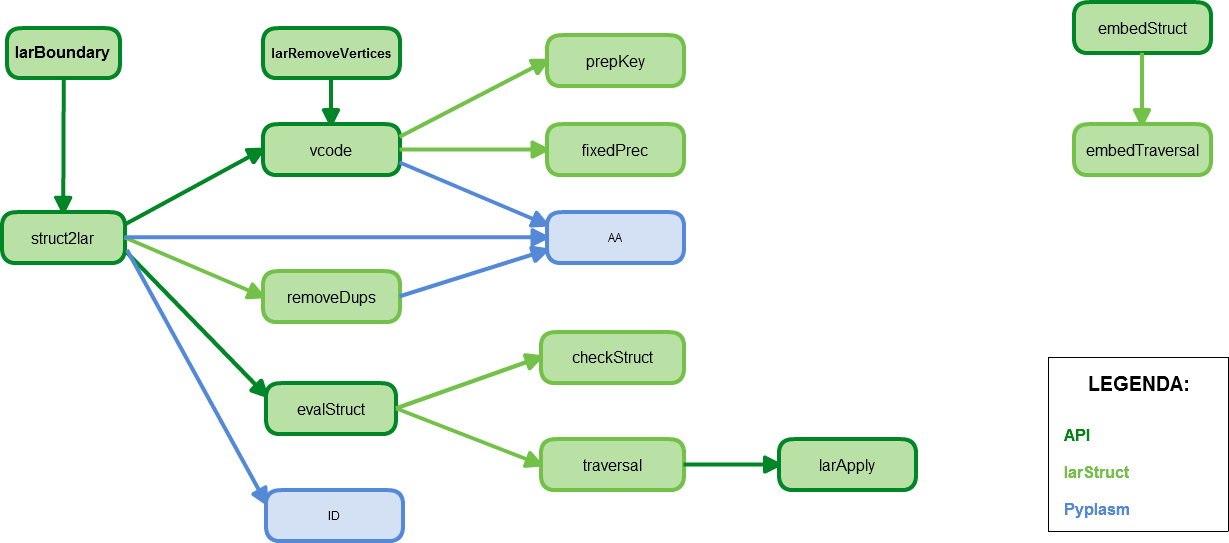
\includegraphics[width=17cm, scale=0.5]{larStruct.png}
\caption[API]{larStruct API}
\end{figure}
%__________________________________________________________________________________________________________________________
\newpage
This module is divided into three sections:\textbf{``Implementation''}, \textbf{``Examples''} and \textbf{``Conclusion''}.

The section ``Implementation'' contains for each function four sub-sections. 
The sub-section \textbf{``Conversion''} shows the conversion of some of the most important functions of the module
from Python to Julia language.
The sub-section \textbf{``Parallelization''} is based on the use of the following Julia's macros to
parallelize the code:
\begin{itemize}

\item \textbf{@everywhere}: can be used to directly define a function on all processes
\item \textbf{@parallel}: can be used to run a for loop on any number of processes
\item \textbf{@sync}: wait until all dynamically-enclosed uses of @async, @spawn, @spawnat and @parallel are complete
\item \textbf{@async}: wraps an expression in a Task and adds it to the local machine's scheduler
queue. Additionally it adds the task to the set of items that the nearest enclosing @sync
waits for.
\end{itemize}
The Parallel computing is performed on 4 simultaneous processes in a personal computer running the command
\begin{Verbatim}[fontsize=\footnotesize]
addprocs(3)
\end{Verbatim}
within Julia console. Alternatively the parallelization can be performed running on the shell the command
\begin{Verbatim}[fontsize=\footnotesize]
julia -p 4
\end{Verbatim}
Parallel computing is performed also on 30 simultaneous processes running the command
\begin{Verbatim}[fontsize=\footnotesize]
addprocs(29)
\end{Verbatim}
within Julia console (in ``Tesla'') or running on the shell the command
\begin{Verbatim}[fontsize=\footnotesize]
julia -p 30
\end{Verbatim}
The main tasks in the sub-section \textbf{``Unit-Test''} are carried out via the use of a particular Julia module, named \textbf{Base.Test}. The latter provides simple unit testing 
functionality. Unit testing is a way to see if your code is correct by checking that the results are what you expect.
It can be helpful to ensure your code still works after you make changes, and can be used when developing as a way of specifying the behaviors your code should have 
when complete.
To perform a simple unit testing, you need first to import the ``Base.Test'' package typing the following command within the Julia console:
\begin{Verbatim}[fontsize=\footnotesize]
using Base.Test
\end{Verbatim}
Then the test can be performed with the @test() macro.

The sub-section \textbf{``Result''} are divided into two parts: in the first part there are the plots representing the execution time of the underlying function performed
on a personal computer with 4 processors. The magnitude of the input is increased by means of the function ``LarCuboids'' (which is imported by the ``largrid'' module):
\begin{Verbatim}[fontsize=\footnotesize]
using PyCall
@pyimport larlib as lar
l=[]
for i in range(0,3)
    p=PyObject(lar.larCuboids([10^i,10^i]))
    push!(l,Tuple(append!([map(collect,PyObject(p[1]))],[PyObject(p[2])])))
    p=PyObject(lar.larCuboids([2*10^i,2*10^i]))
    push!(l,Tuple(append!([map(collect,PyObject(p[1]))],[PyObject(p[2])])))
    p=PyObject(lar.larCuboids([5*10^i,5*10^i]))
    push!(l,Tuple(append!([map(collect,PyObject(p[1]))],[PyObject(p[2])])))
end
\end{Verbatim}
The function used to compute the execution time is:
 \begin{Verbatim}[fontsize=\footnotesize]
function Time(f,args)
    @elapsed f(args...)
    t=[]
    for i in range(1,10)
	push!(t,@elapsed f(args...))
    end
    m=mean(t)
    return m
end
\end{Verbatim}
The macro @elapsed is used to evaluates the execution time of the function given in input, discarding the resulting value, and returning just the amount of seconds elapsed
to run the function. The time is expressed as a floating-point number. 

The second part of the subsection “Result” contains the plot of the underlying function performance, 
run on “Tesla” with 30 processors, where the input magnitute is increased via the following function:
\begin{Verbatim}[fontsize=\footnotesize]
function addn2D(n,model)
  body=[]
  for i in range(1,n)
    el=[]
    matrix=rand(1:3)
    if matrix==1
      x=rand(1:10)/10
      y=rand(1:10)/10
      append!(el,larApply(t(x,y))(model))
      append!(body,[el])
    elseif matrix ==2
      x=rand(1:10)/10
      y=rand(1:10)/10
      append!(el,larApply(s(x,y))(model))
      append!(body,[el])
    elseif matrix ==3
      x=rand(1:10)
      append!(el,larApply(r(pi/x))(model))
      append!(body,[el])
    end
  end
  a=Struct(body)
  return a
end
\end{Verbatim}
To generate the plots you need to import ``Plots'' and ``Distributions'' packages typing the following commands within the Julia console:
\begin{itemize}
 \item 
 \begin{Verbatim}[fontsize=\footnotesize]
  using Plots
 \end{Verbatim}
 \item
 \begin{Verbatim}[fontsize=\footnotesize]
  using Distributions
 \end{Verbatim}
\end{itemize}
%__________________________________________________________________________________________________________________________
\newpage

\section{Implementation}
\subsection{checkStruct}
\subsubsection{Conversion}
\framebox[5em][c]{\textbf{\normalsize Python}}

\begin{Verbatim}[fontsize=\footnotesize]
def checkStruct(lst):
    obj = lst[0]
    if(isinstance(obj,tuple) or isinstance(obj,list)):
	dim = len(obj[0][0])
    elif isinstance(obj,Model):
	dim = obj.n
    elif isinstance(obj,Mat):
	dim = obj.shape[0]-1
    elif isinstance(obj,Struct):
	dim = len(obj.box[0])    
return dim
\end{Verbatim}
\framebox[5em][c]{\textbf{\normalsize Julia}}

\begin{Verbatim}[fontsize=\footnotesize]
function checkStruct(lst)
  obj = lst[1]
  if isa(obj,Matrix)
      dim=size(obj)[1]-1
  elseif(isa(obj,Tuple) || isa(obj,Array))
      dim=length(obj[1][1])
  elseif isa(obj,Struct)
      dim=length(obj.box[1])
  end 
  return dim
end
\end{Verbatim}

\subsubsection{Parallelization}
\begin{Verbatim}[fontsize=\footnotesize]
function pcheckStruct(lst)
  obj = lst[1]
  if isa(obj,Matrix)
    dim=size(obj)[1]-1 
  elseif(isa(obj,Tuple) || isa(obj,Array))
    dim=length(obj[1][1])
  elseif isa(obj,pStruct)
    dim=length(obj.box[1])
  end
  return dim
end
\end{Verbatim}

\subsubsection{Unit-Test}
\begin{Verbatim}[fontsize=\footnotesize]
@testset "checkStruct Tests" begin
  list=([[0.575,-0.175],[0.575,0.175],[0.925,-0.175],[0.925,0.175]],[[0,1,2,3]])
@test checkStruct(list)==length(list[1][1][1])
@test typeof(checkStruct(list))==Int
end
\end{Verbatim}

%______________________________________________________________________________________________________________________________

\newpage
\subsection{larApply}
\subsubsection{Conversion}
The function larApply returns as output an affine trasformation of the input object and it is based on the following affine matrices:
\vspace{10px}

\noindent\framebox[42em][c]{Rotation}
\begin{multicols}{2}
\noindent \framebox[5em][c]{\textbf{\normalsize Python}}
\begin{Verbatim}[fontsize=\scriptsize]
def r(*args):
  args = list(args)
  n = len(args)
  if n == 1: # rotation in 2D
    angle = args[0]; cos = COS(angle); sin = SIN(angle)
    mat = scipy.identity(3)
    mat[0,0] = cos;    mat[0,1] = -sin;
    mat[1,0] = sin;    mat[1,1] = cos;
  if n == 3: # rotation in 3D
    mat = scipy.identity(4)
    angle = VECTNORM(args); axis = UNITVECT(args)
    cos = COS(angle); sin = SIN(angle)
    if axis[1]==axis[2]==0.0:    # rotation about x
      mat[1,1] = cos;    mat[1,2] = -sin;
      mat[2,1] = sin;    mat[2,2] = cos;
    elif axis[0]==axis[2]==0.0:    # rotation about y
      mat[0,0] = cos;    mat[0,2] = sin;
      mat[2,0] = -sin;    mat[2,2] = cos;
    elif axis[0]==axis[1]==0.0:    # rotation about z
      mat[0,0] = cos;    mat[0,1] = -sin;
      mat[1,0] = sin;    mat[1,1] = cos;
    else:  # general 3D rotation
      I = scipy.identity(3) ; u = axis
      Ux = scipy.array([
	  [0,        -u[2],      u[1]]
	  [u[2],        0,     -u[0]],
	  [-u[1],     u[0],         0]])
      UU = scipy.array([
	  [u[0]*u[0],    u[0]*u[1],    u[0]*u[2]],
	  [u[1]*u[0],    u[1]*u[1],    u[1]*u[2]],
	  [u[2]*u[0],    u[2]*u[1],    u[2]*u[2]]])
	  mat[:3,:3] = cos*I + sin*Ux + (1.0-cos)*UU
return mat.view(Mat)
\end{Verbatim}
\columnbreak
\framebox[5em][c]{\textbf{\normalsize Julia}}
\begin{Verbatim}[fontsize=\scriptsize]
  function r(args...)
    args = collect(args)
    n = length(args)
    if n == 1 # rotation in 2D
      angle = args[1]; COS = cos(angle); SIN = sin(angle)
      mat = eye(3)
      mat[1,1] = COS;    mat[1,2] = -SIN;
      mat[2,1] = SIN;    mat[2,2] = COS;
    end
    if n == 3 # rotation in 3D
      mat = eye(4)
      angle = norm(args); axis = normalize(args)
      COS = cos(angle); SIN= sin(angle)
      if axis[2]==axis[3]==0.0    # rotation about x
	mat[2,2] = COS;    mat[2,3] = -SIN;
	mat[3,2] = SIN;    mat[3,3] = COS;
      elseif axis[1]==axis[3]==0.0   # rotation about y
	mat[1,1] = COS;    mat[1,3] = SIN;
	mat[3,1] = -SIN;    mat[3,3] = COS;
      elseif axis[1]==axis[2]==0.0    # rotation about z
	mat[1,1] = SIN;    mat[1,2] = -SIN;
	mat[2,1] = COS;    mat[2,2] = COS;
      else
	I=eye(3); u=axis
	Ux=[0 -u[3] u[2] ; u[3] 0 -u[1] ;  -u[2] u[1] 1]
	UU =[u[1]*u[1]    u[1]*u[2]   u[1]*u[3];
	    u[2]*u[1]    u[2]*u[2]   u[2]*u[3];
	    u[3]*u[1]    u[3]*u[2]   u[3]*u[3]]
	mat[1:3,1:3]=COS*I+SIN*Ux+(1.0-COS)*UU
      end
    end
  return mat
  end
\end{Verbatim}
\end{multicols}
\framebox[42em][c]{Translation}
\begin{multicols}{2}
\framebox[5em][c]{\textbf{\normalsize Python}}
\begin{Verbatim}[fontsize=\scriptsize]
    def t(*args):
      d = len(args)
      mat = scipy.identity(d+1)
      for k in range(d):
	mat[k,d] = args[k]
      return mat.view(Mat)   
\end{Verbatim}
\columnbreak
\framebox[5em][c]{\textbf{\normalsize Julia}}
\begin{Verbatim}[fontsize=\scriptsize]

 function t(args...)
   d=length(args)
   mat=eye(d+1)
   for k in range(1,d)
     mat[k,d+1]=args[k]
   end
   return mat
 end

\end{Verbatim}
\end{multicols}
\noindent \framebox[42em][c]{Scaling}
\begin{multicols}{2}
\noindent \framebox[5em][c]{\textbf{\normalsize Python}}
\begin{Verbatim}[fontsize=\scriptsize]
def s(*args):
  d = len(args)
  mat = scipy.identity(d+1)
  for k in range(d):
    mat[k,k] = args[k]
  return mat.view(Mat)
    
\end{Verbatim}
\columnbreak
\framebox[5em][c]{\textbf{\normalsize Julia}}
\begin{Verbatim}[fontsize=\scriptsize]
function s(args...)
  d=length(args)
  mat=eye(d+1)
  for k in range(1,d)
    mat[k,k]=args[k]
  end
  return mat
end
\end{Verbatim}
\end{multicols}
\noindent \framebox[5em][c]{\textbf{\normalsize Python}}
\begin{Verbatim}[fontsize=\footnotesize]
def larApply(affineMatrix);
  def larApply0(model):
    if isinstance(model,Model):
      V = scipy.dot(array([v+[1.0] for v in model.verts]),affineMatrix.T).tolist()
      V = [v[:-1] for v in V]
      CV = copy.copy(model.cells)
      return Model((V,CV))
    elif isinstance(model,tuple) or isinstance(model,list):
      if len(model)==2: V,CV = model
      elif len(model)==3: V,CV,FV = model
      V=scipy.dot([list(v)+[1.0]for v in V],affineMatrix.T).tolist()
      if len(model)==2: return [v[:-1] for v in V],CV
      elif len(model)==3: return [v[:-1] for v in V],CV,FV
  return larApply0
\end{Verbatim}

\noindent \framebox[5em][c]{\textbf{\normalsize Julia}}
\begin{Verbatim}[fontsize=\footnotesize]
function larApply(affineMatrix)
  function larApply0(model)
    if length(model)==2
      V,CV=model
    elseif length(model)==3
      V,CV,FV = model
    end
    V1=Array{Float64}[]
    for (k,v) in enumerate(V)
      append!(v,[1.0])
      push!(V1,vec((v')*transpose(affineMatrix)))
      pop!(V[k])
      pop!(V1[k])
    end
    if length(model)==2
      return V1,CV
    elseif length(model)==3
      return V1,CV,FV
    end
   end 
   return larApply0
end
\end{Verbatim}
\subsubsection{Parallelization}
The affine transformation matrices are the same as in the sequential case.

\begin{Verbatim}[fontsize=\footnotesize]
@everywhere function plarApply(affineMatrix)
  function plarApply0(model)
    if length(model)==2
      V,CV=deepcopy(model)
    elseif length(model)==3
      V,CV,FV = deepcopy(model)
    end
    V1=Array{Float64}[]
    V1=@sync @parallel (append!)for v in V
      append!(v,[1.0])
      [collect(vec((v')*transpose(affineMatrix)))]
    end
    for v in V1
      pop!(v)
    end
    if length(model)==2
      return fetch(V1),CV
    elseif length(model)==3
      return V1,CV,FV
    end
  end
  return plarApply0
end
\end{Verbatim}
\subsubsection{Unit-Test}

\framebox[42em][c]{Serial Tests}
\begin{Verbatim}[fontsize=\footnotesize]
square=([[0,0],[0,1],[1,0],[1,1]],[[0,1,2,3]])
cubes=([[0,0,0],[0,0,1],[0,1,0],[0,1,1],[1,0,0],[1,0,1],[1,1,0],[1,1,1]],[[0,1,2,3,4,5,6,7]])

@testset "larApply Tests" begin
  @testset "2D" begin
    @testset "larApply Translation 2D" begin
      @test typeof(larApply(t(-0.5,-0.5))(square))==Tuple{Array{Array{Float64,N} where N,1},
      Array{Array{Int64,1},1}}
      @test larApply(t(-0.5,-0.5))(square)==([[-0.5,-0.5],[-0.5,0.5],[0.5,-0.5],[0.5,0.5]],
      [[0,1,2,3]])
    end
    
    @testset "larApply Scaling 2D" begin
      @test typeof(larApply(s(-0.5,-0.5))(square))==Tuple{Array{Array{Float64,N} where N,1},
      Array{Array{Int64,1},1}}
      @test larApply(s(-0.5,-0.5))(square)==([[0.0,0.0],[0.0,-0.5],[-0.5,0.0],[-0.5,-0.5]],
      [[0,1,2,3]])
    end
    
    @testset "larApply Rotation 2D" begin
      @test typeof(larApply(r(0))(square))==Tuple{Array{Array{Float64,N}  where N,1},
      Array{Array{Int64,1},1}}
      @test larApply(r(0))(square)==square
    end
  end
  
  @testset "3D" begin
    @testset "larApply Translation 3D" begin
      @test typeof(larApply(t(-0.5,-0.5,-0.5))(cubes))==Tuple{Array{Array{Float64,N}
      where N,1},Array{Array{Int64,1},1}}
      @test larApply(t(-0.5,-0.5,-0.5))(cubes)==([[-0.5,-0.5,-0.5],[-0.5,-0.5,0.5],
      [-0.5,0.5,-0.5],
      [-0.5,0.5,0.5],[0.5,-0.5,-0.5],[0.5,-0.5,0.5],[0.5,0.5,-0.5],[0.5,0.5,0.5]],
      [[0,1,2,3,4,5,6,7]])
    end
    
    @testset "larApply Scaling 3D" begin
      @test typeof(larApply(s(-0.5,-0.5,-0.5))(cubes))==Tuple{Array{Array{Float64,N} 
      where N,1},Array{Array{Int64,1},1}}
      @test larApply(s(-0.5,-0.5,-0.5))(cubes)==([[0.0,0.0,0.0],[0.0,0.0,-0.5],[0.0,-0.5,0.0],
      [0.0,-0.5,-0.5],[-0.5,0.0,0.0],[-0.5,0.0,-0.5],[-0.5,-0.5,0.0],[-0.5,-0.5,-0.5]],
      [[0,1,2,3,4,5,6,7]])
    end
    
    @testset "larApply Rotation 3D" begin
      @test typeof(larApply(r(pi,0,0))(cubes))==Tuple{Array{Array{Float64,N} where N,1},
      Array{Array{Int64,1},1}}
      @test isapprox(larApply(r(pi,0,0))(cubes)[1],[[0.0,0.0,0.0],[0.0,-1.22465e-16,-1.0],
      [0.0,-1.0,1.22465e-16],[0.0,-1.0,-1.0],[1.0,0.0,0.0],[1.0,-1.22465e-16,-1.0],
      [1.0,-1.0,1.22465e-16],[1.0,-1.0,-1.0]])
    end
  end
end
\end{Verbatim}

\noindent \framebox[42em][c]{Parallel Tests}
\begin{Verbatim}[fontsize=\footnotesize]
square=([[0,0],[0,1],[1,0],[1,1]],[[0,1,2,3]])
cubes=([[0,0,0],[0,0,1],[0,1,0],[0,1,1],[1,0,0],[1,0,1],[1,1,0],[1,1,1]],[[0,1,2,3,4,5,6,7]])
@testset "plarApply Tests" begin
  @testset "2D" begin
    @testset "plarApply Translation 2D" begin
      @test typeof(plarApply(t(-0.5,-0.5))(square))==Tuple{Array{Array{Float64,1},1},
      Array{Array{Int64,1},1}}
      @test plarApply(t(-0.5,-0.5))(square)==([[-0.5,-0.5],[-0.5,0.5],[0.5,-0.5],[0.5,0.5]],
      [[0,1,2,3]])
    end
    @testset "plarApply Scaling 2D" begin
      @test typeof(plarApply(s(-0.5,-0.5))(square))==Tuple{Array{Array{Float64,1},1},
      Array{Array{Int64,1},1}}
      @test plarApply(s(-0.5,-0.5))(square)==([[0.0,0.0],[0.0,-0.5],[-0.5,0.0],
      [-0.5,-0.5]],[[0,1,2,3]])
    end
    @testset "plarApply Rotation 2D" begin
      @test typeof(plarApply(r(0))(square))==Tuple{Array{Array{Float64,1},1},
      Array{Array{Int64,1},1}}
      @test plarApply(r(0))(square)==square
    end
  end
  @testset "3D" begin
    @testset "plarApply Translation 3D" begin
    @test typeof(plarApply(t(-0.5,-0.5,-0.5))(cubes))==Tuple{Array{Array{Float64,1},1},
    Array{Array{Int64,1},1}}
    @test plarApply(t(-0.5,-0.5,-0.5))(cubes)==([[-0.5,-0.5,-0.5],[-0.5,-0.5,0.5],[-0.5,0.5,-0.5],
    [-0.5,0.5,0.5],[0.5,-0.5,-0.5],[0.5,-0.5,0.5],[0.5,0.5,-0.5],[0.5,0.5,0.5]],[[0,1,2,3,4,5,6,7]])
  end 
    @testset "plarApply Scaling 3D" begin
      @test typeof(plarApply(s(-0.5,-0.5,-0.5))(cubes))==Tuple{Array{Array{Float64,1},1},
      Array{Array{Int64,1},1}}
      @test plarApply(s(-0.5,-0.5,-0.5))(cubes)==([[0.0,0.0,0.0],[0.0,0.0,-0.5],[0.0,-0.5,0.0],
      [0.0,-0.5,-0.5],[-0.5,0.0,0.0],[-0.5,0.0,-0.5],[-0.5,-0.5,0.0],[-0.5,-0.5,-0.5]],
      [[0,1,2,3,4,5,6,7]])
    end
    @testset "plarApply Rotation 3D" begin
      @test typeof(plarApply(r(pi,0.0,0.0))(cubes))==Tuple{Array{Array{Float64,1},1},
      Array{Array{Int64,1},1}}
      @test isapprox(plarApply(r(pi,0,0))(cubes)[1],[[0.0,0.0,0.0],[0.0,-1.22465e-16,-1.0],
      [0.0,-1.0,-1.22465e-16],[0.0,-1.0,-1.0],
      [1.0,0.0,0.0],[1.0,-1.22465e-16,-1.0],[1.0,-1.0,1.22465e-16],[1.0,-1.0,-1.0]])
    end
  end
end
\end{Verbatim}

\subsubsection{Results}
\textbf{Execution time on PC}
\begin{Verbatim}[fontsize=\footnotesize]
times=[]
ptimes=[]
append!(ptimes,Time(plarApply(t(-0.5,-0.5)),[l[i]]) for i in range(1,length(l)))
append!(ptimes,Time(plarApply(t(-0.5,-0.5)),[l[i]]) for i in range(1,length(l)))

plot(times,xlabel="input",xlims=(0,length(times)+2),ylabel="time(s)",label=["Serial"])
plot(ptimes,xlabel="input",xlims=(0,length(times)+2),ylabel="time(s)",label=["Parallel"])
\end{Verbatim}

\begin{figure*}[!h]
\centering
\subfloat[Serial]{%
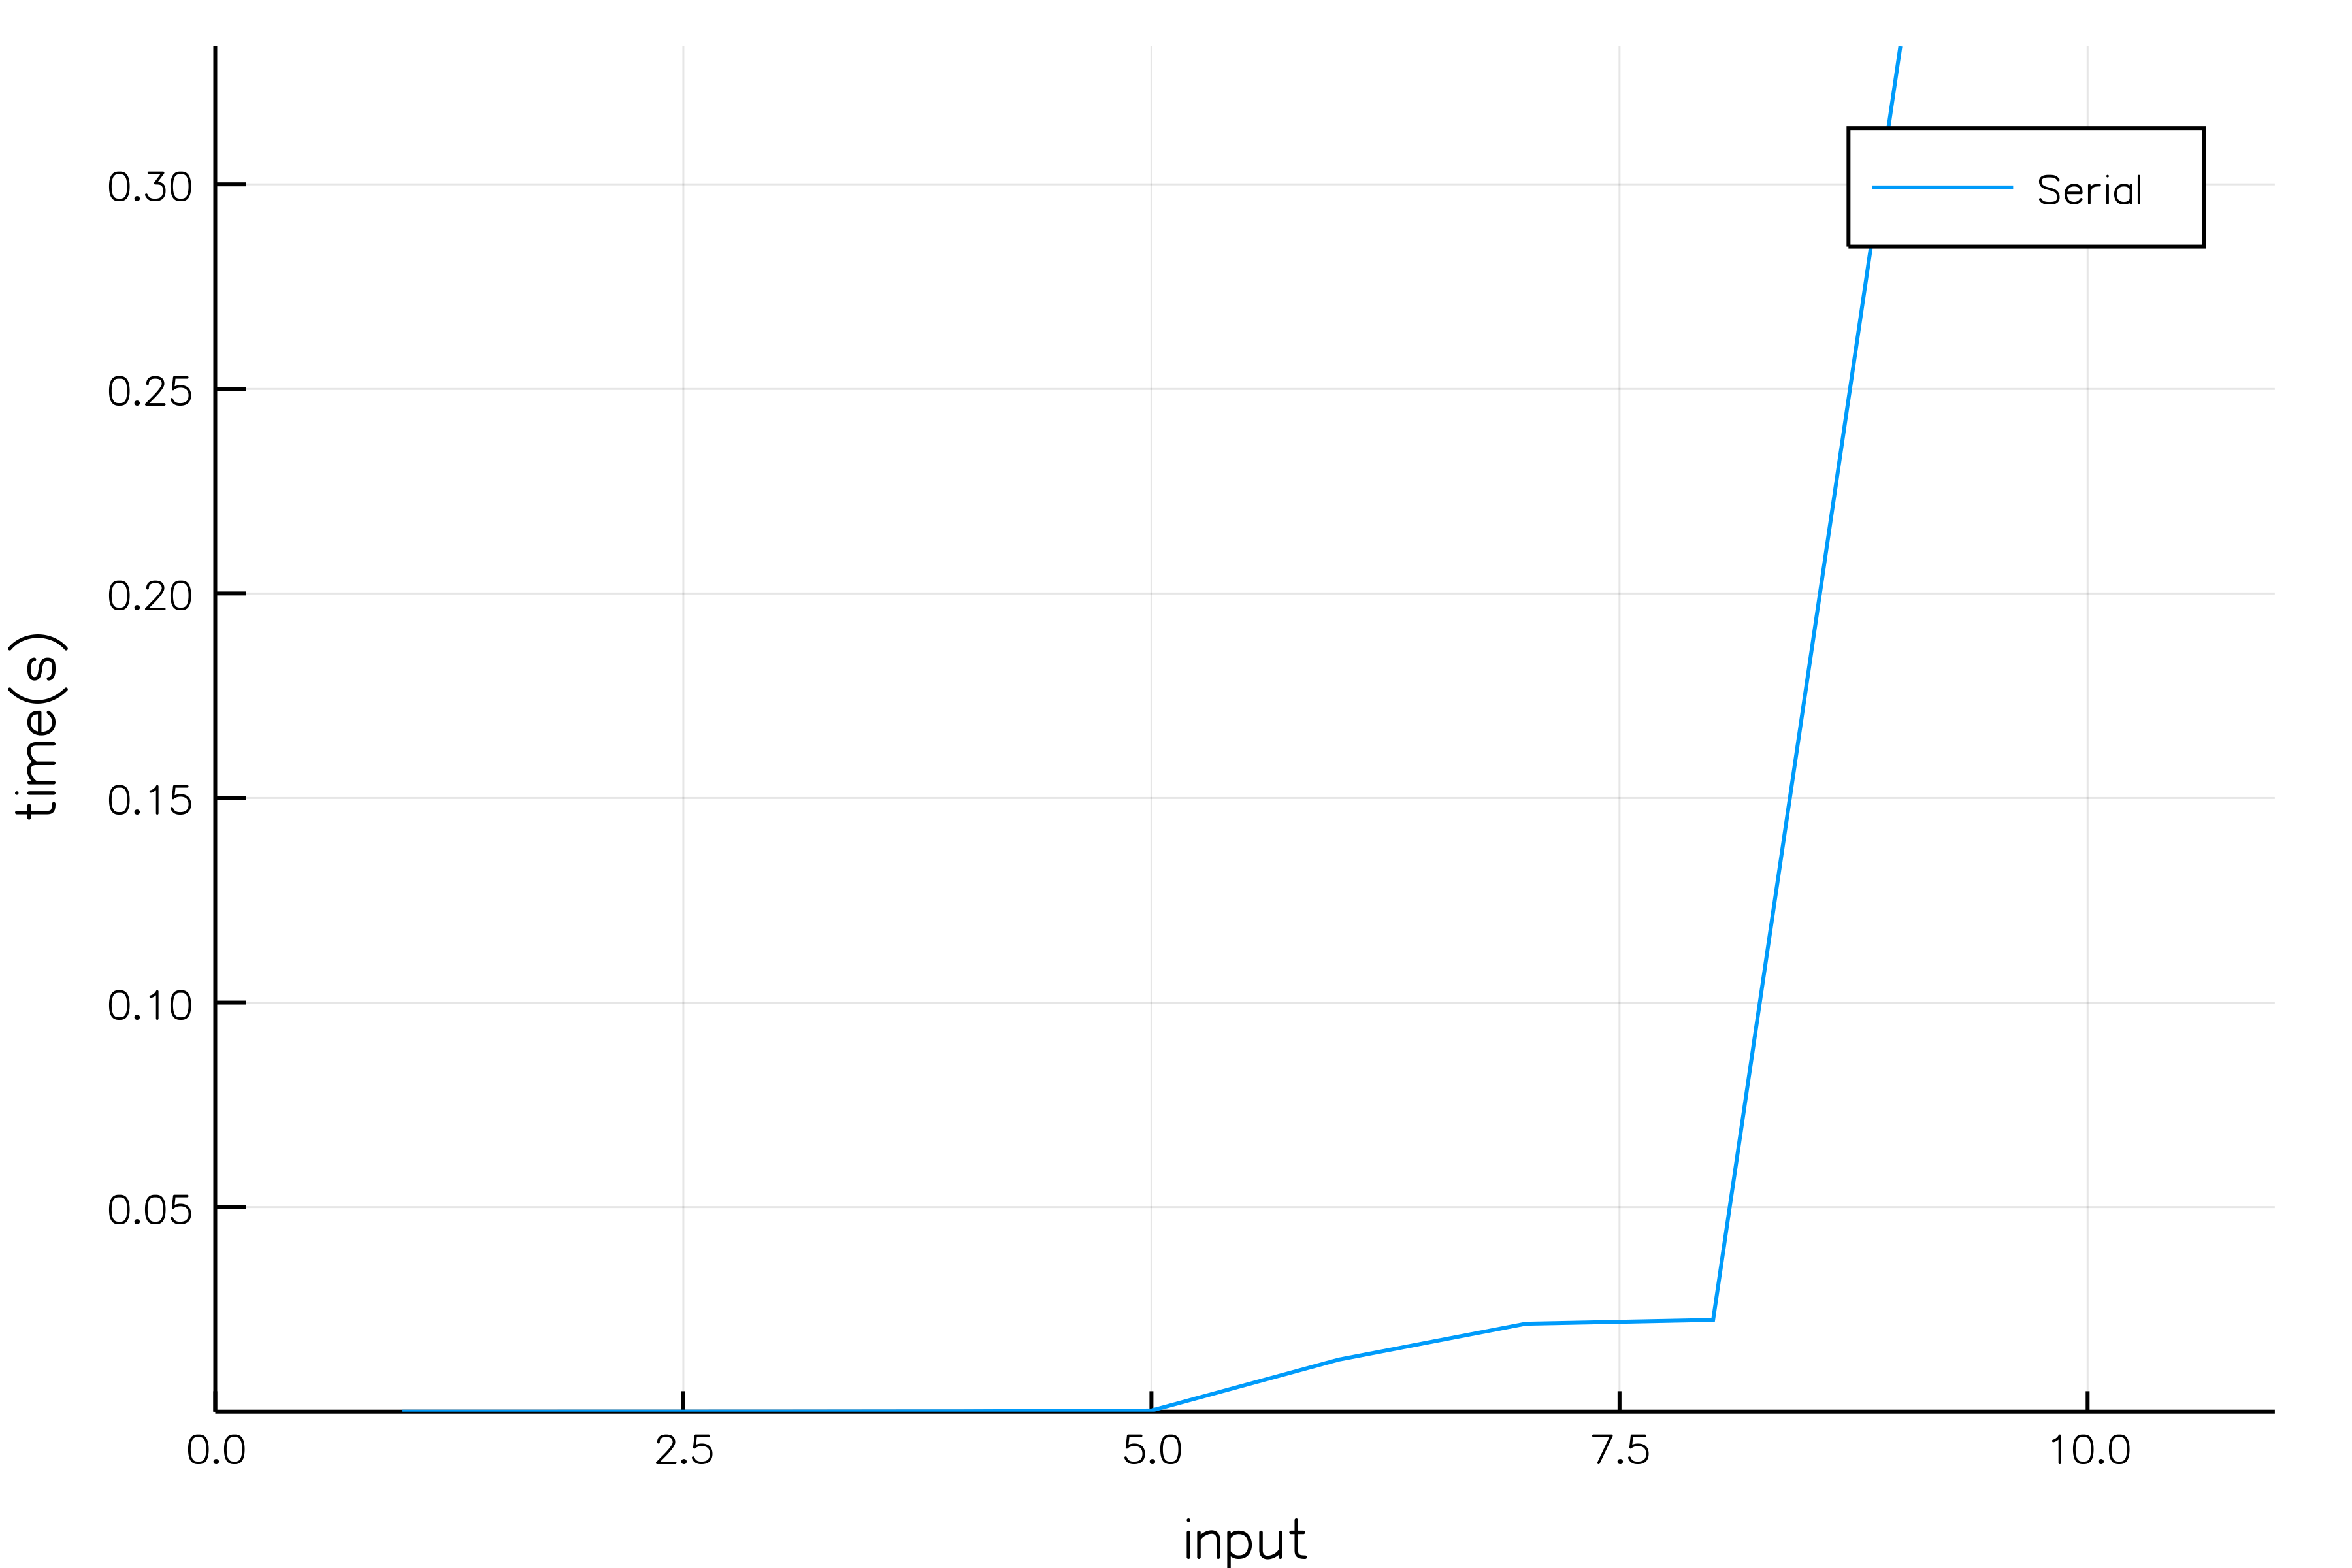
\includegraphics[scale=0.060]{larApplySerial.png}
}
\subfloat[Parallel]{%
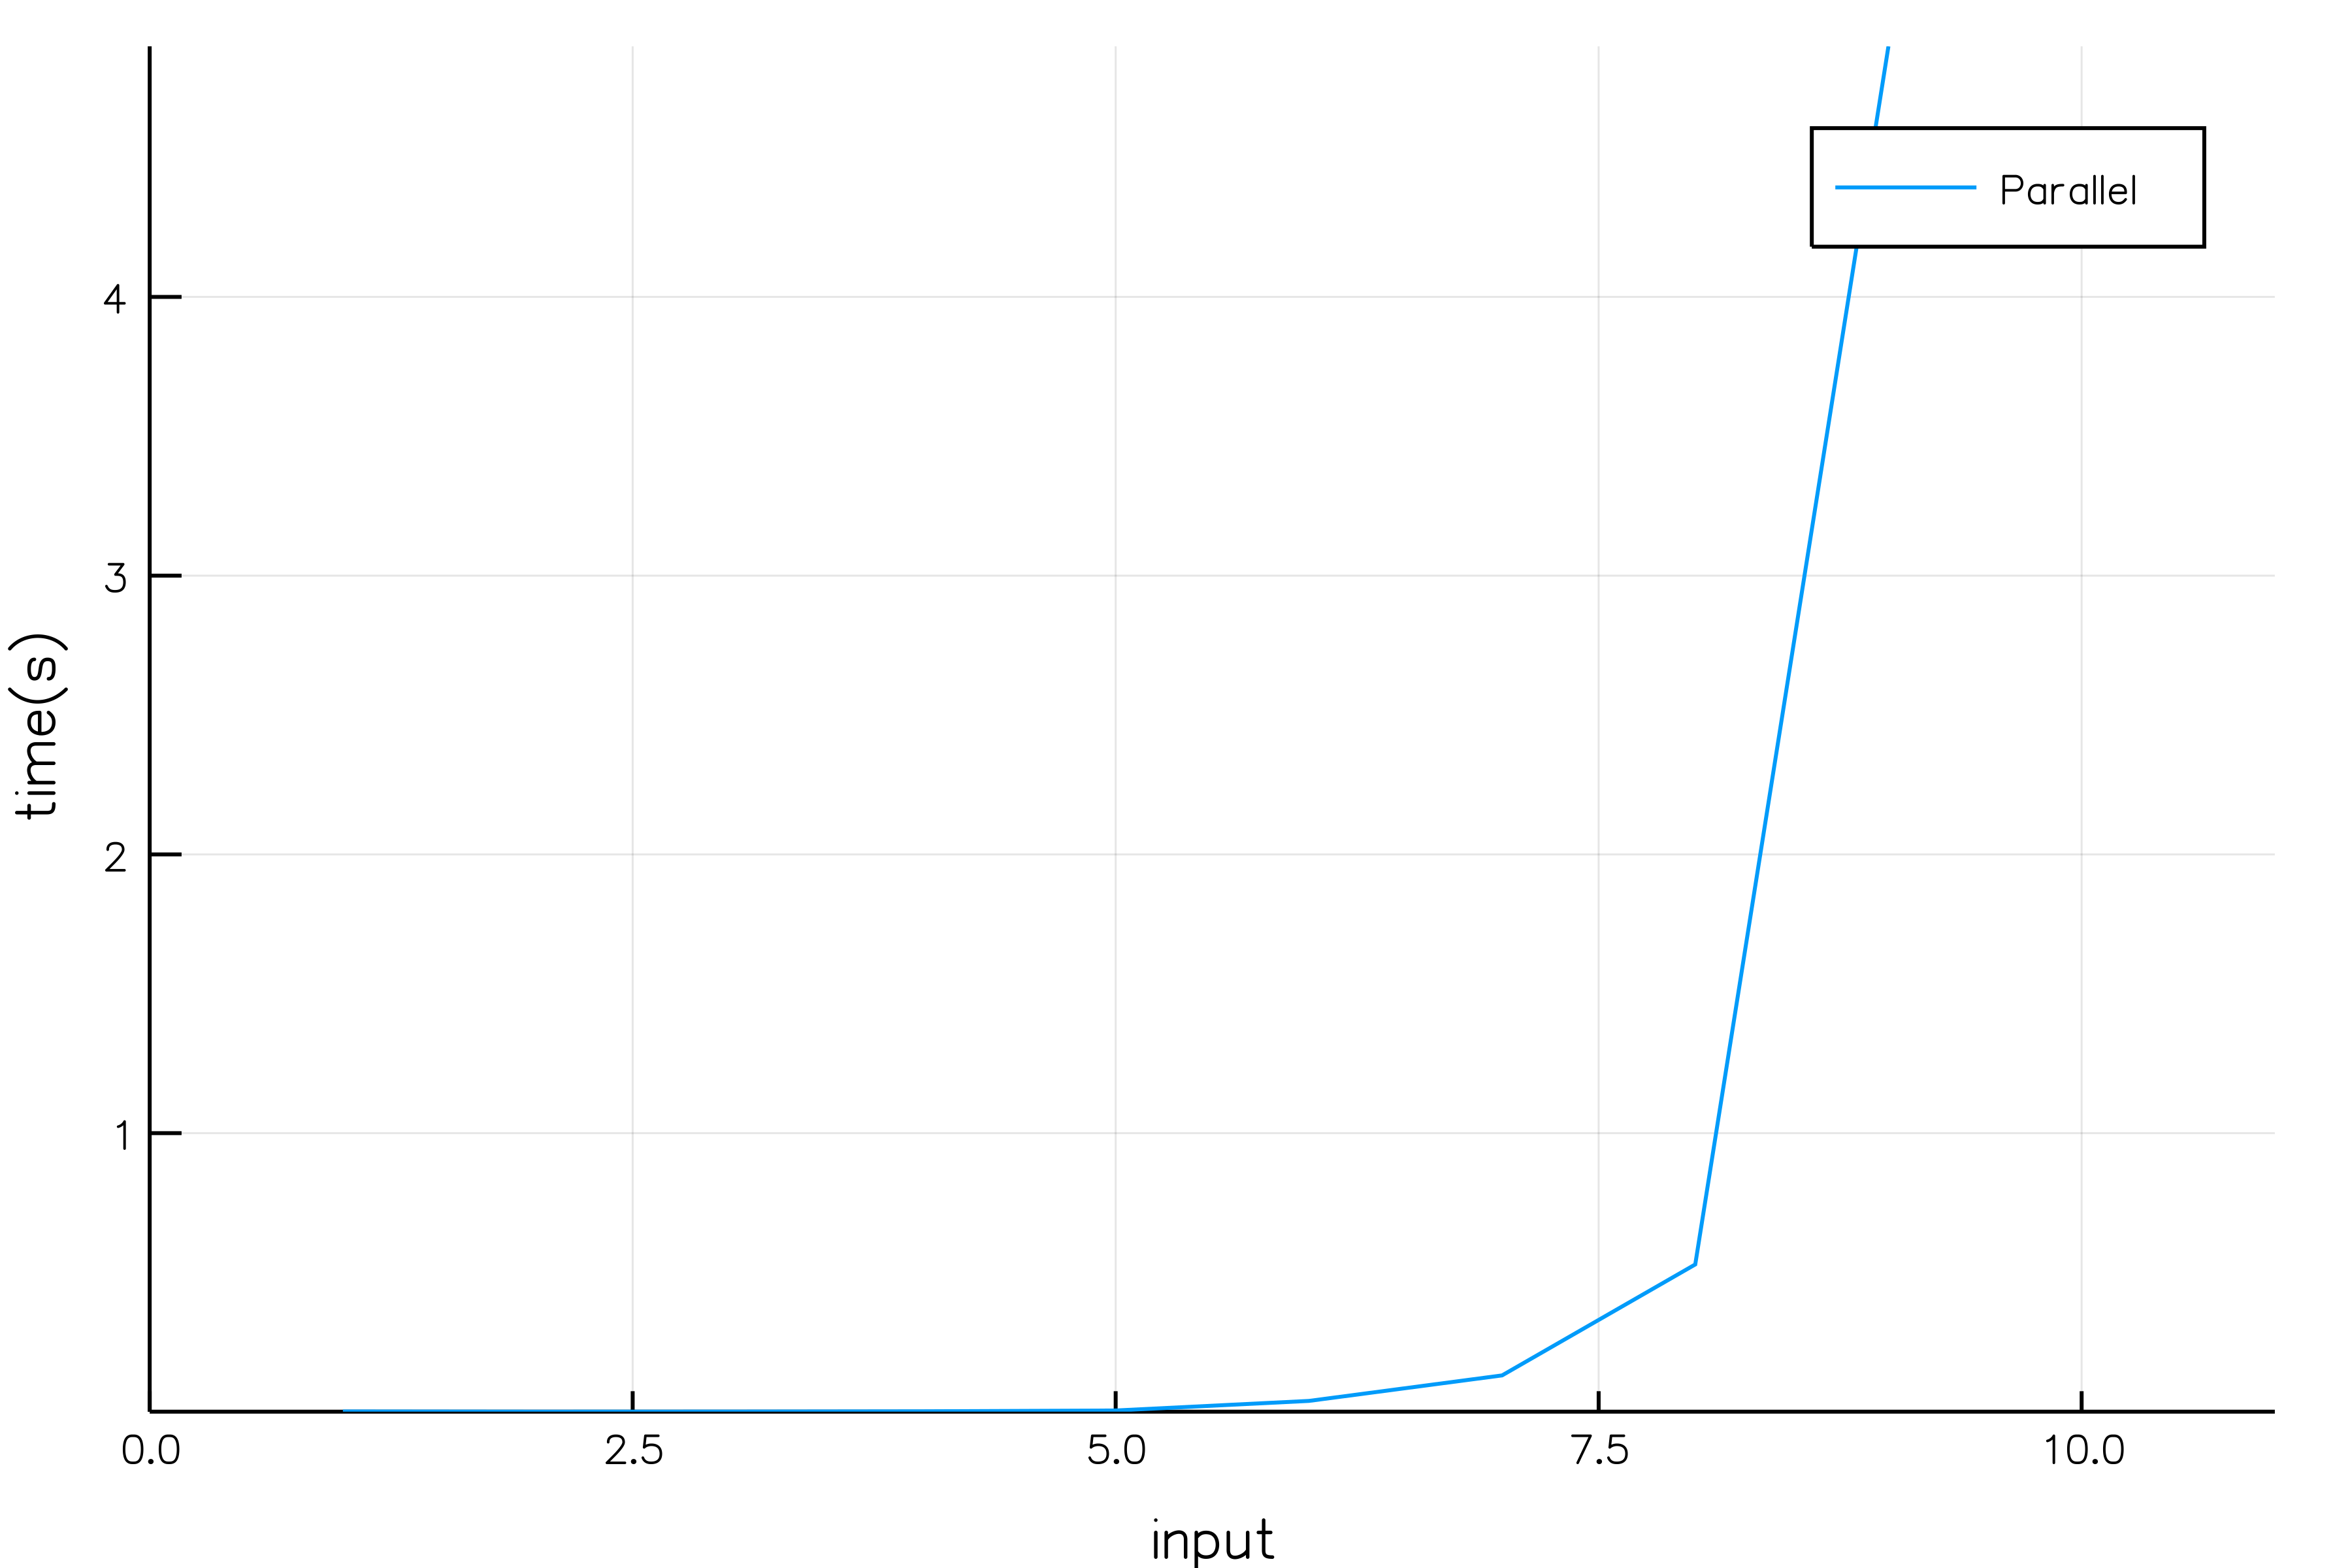
\includegraphics[scale=0.060]{larApplyParallel.png}
}
\caption{Execution time of function larApply}
\end{figure*}
\vspace{25px}
\noindent \framebox[42em][c]{Compare}
\begin{Verbatim}[fontsize=\footnotesize]
plot([times,ptimes],xlabel="input",xlims=(0,length(times)+2),ylabel="time(s)",
label=["Serial","Parallel"])
\end{Verbatim}
\begin{figure}[!h]
\centering
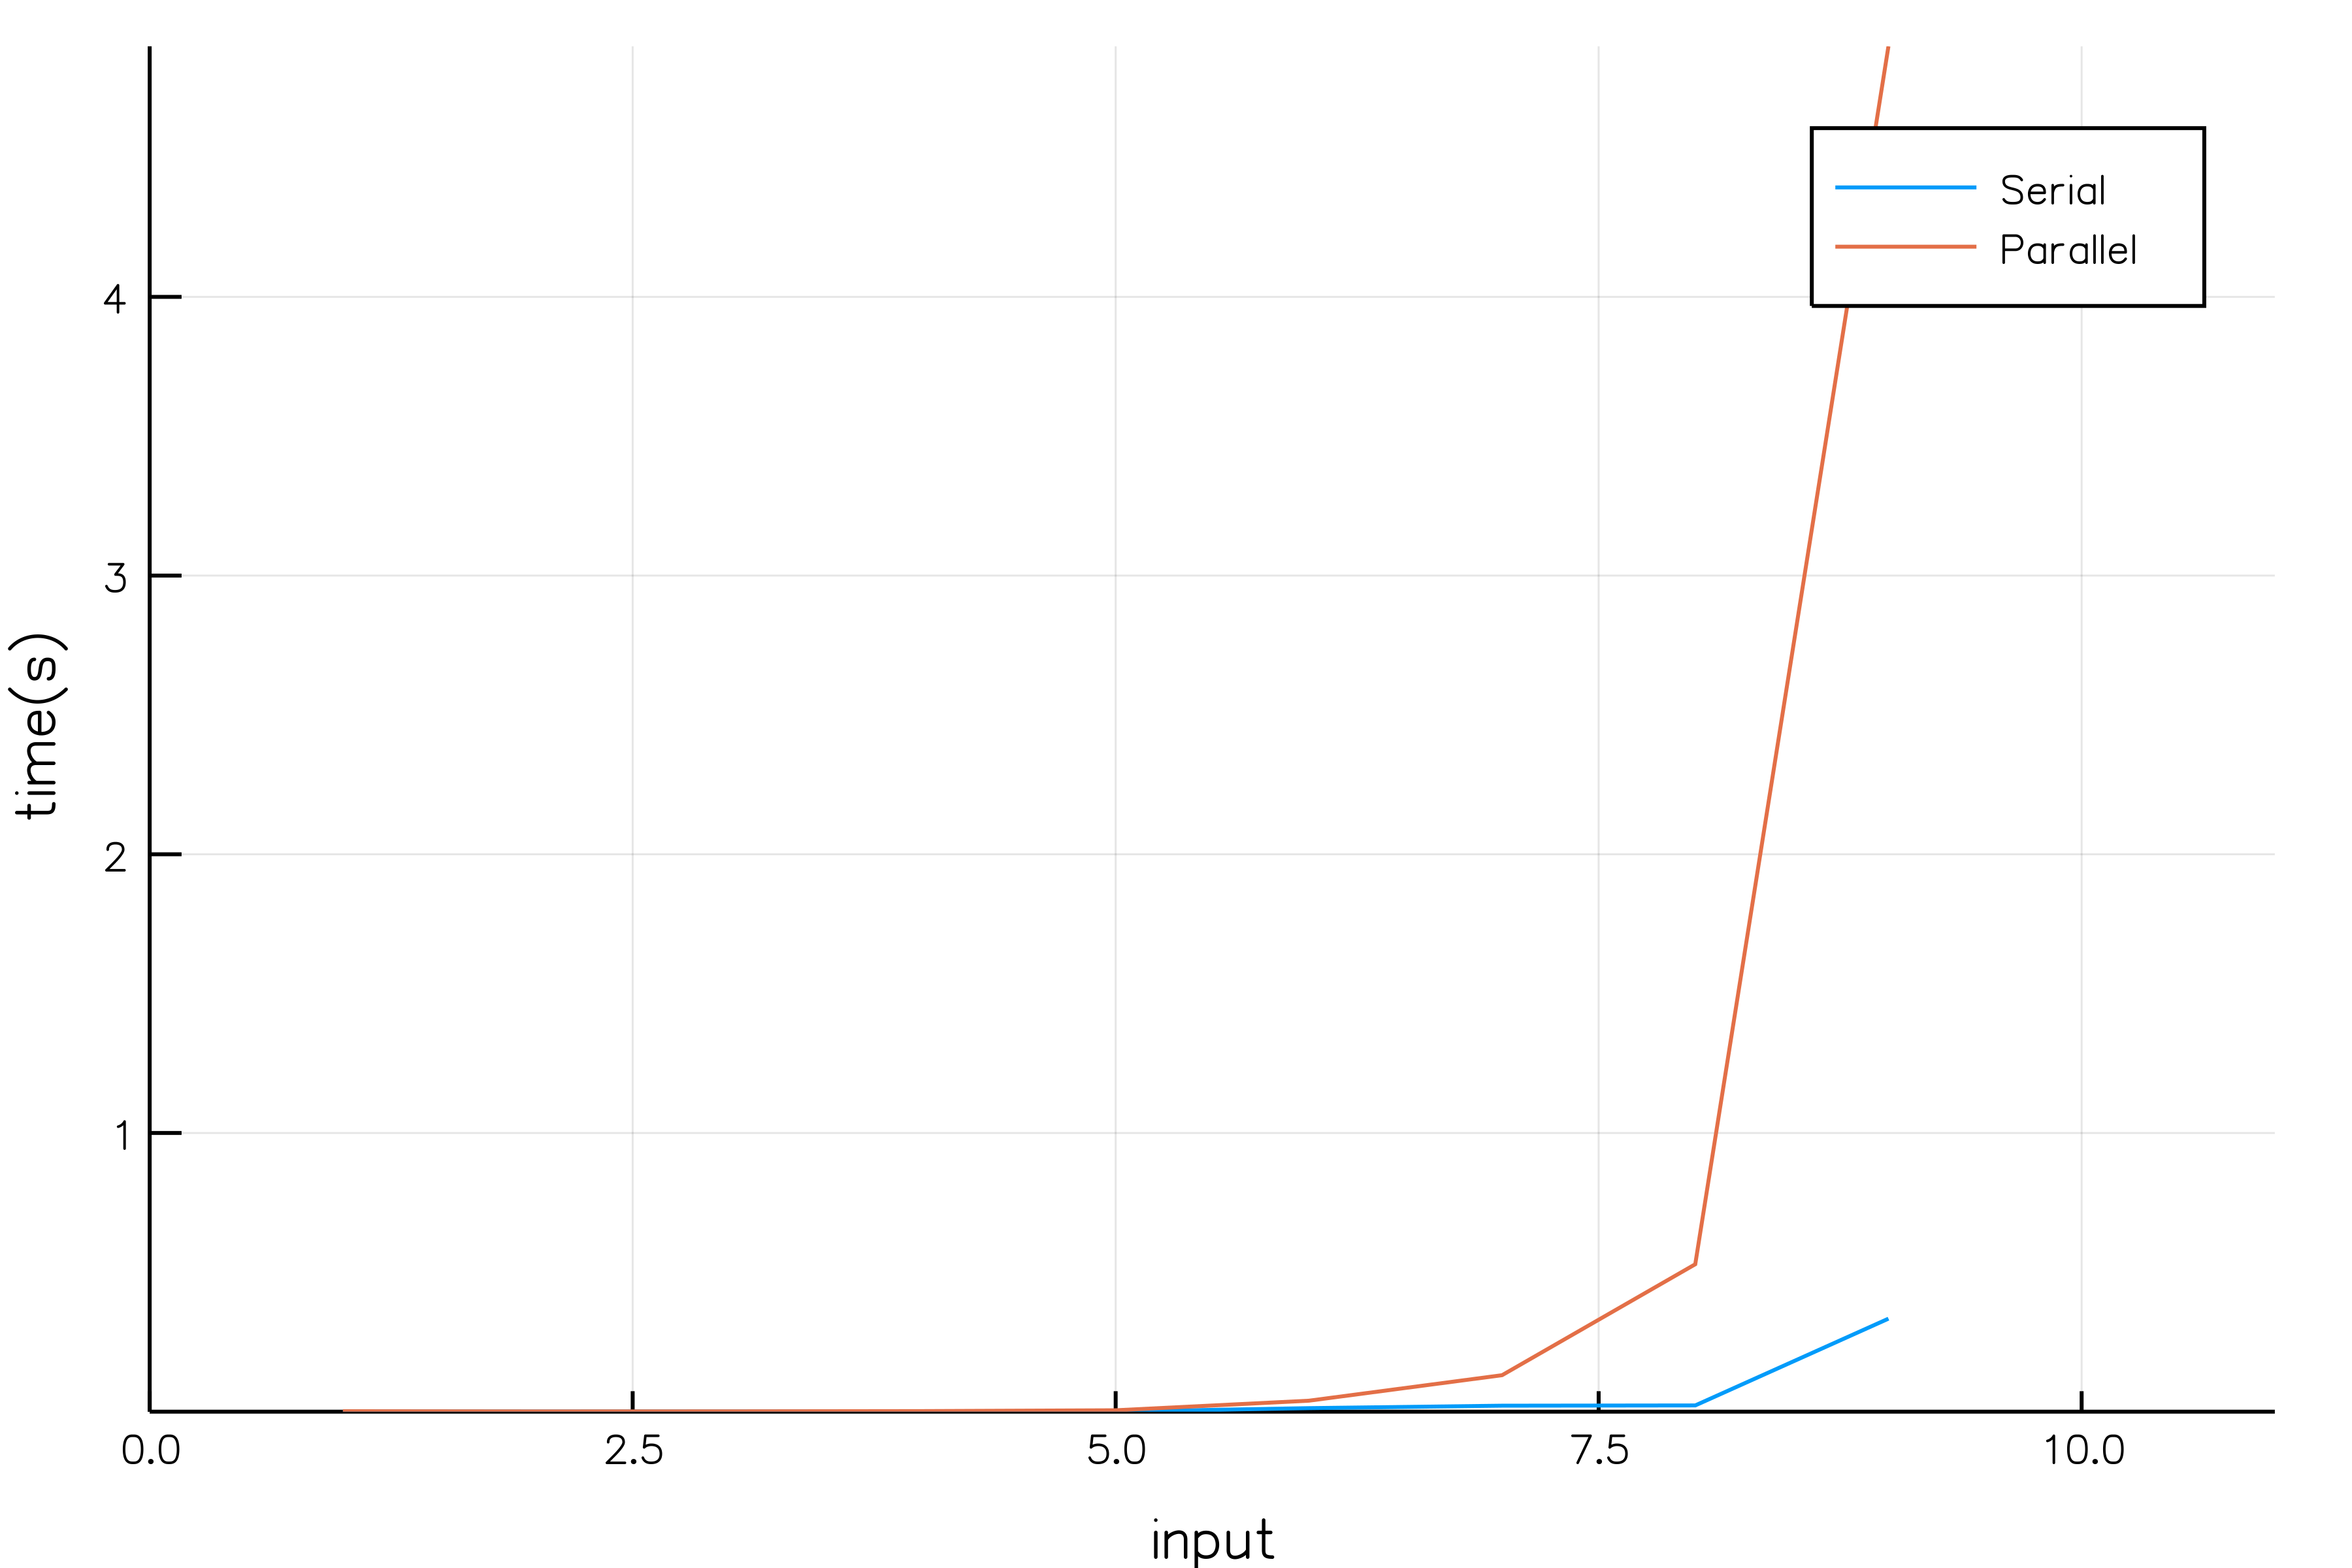
\includegraphics[scale=0.08]{larApplyC.png}
\caption{Compare Parallel and Serial execution time of function larApply}
\end{figure}
\newpage

%_________________________________________________________________________________________________________________________________-

\subsection{box}
\subsubsection{Conversion}
\framebox[5em][c]{\textbf{\normalsize Python}}
\begin{Verbatim}[fontsize=\footnotesize]
def box(model):
  if isinstance(model,Mat): return []
  elif isinstance(model,Struct):
    dummyModel = copy.deepcopy(model)
    dummyModel.body = [term if (not isinstance(term,Struct))
  else [term.box,[[0,1]]]  for term in model.body]
    listOfModels = evalStruct( dummyModel )
    theMin,theMax = box(listOfModels[0])
    for theModel in listOfModels[1:]:
      modelMin, modelMax = box(theModel)
      theMin = [val if val<theMin[k] else theMin[k] for k,val in enumerate(modelMin)]
      theMax = [val if val>theMax[k] else theMax[k] for k,val in enumerate(modelMax)]
    return [theMin,theMax]
  elif isinstance(model,Model):
    V = model.verts
  elif (isinstance(model,tuple) or isinstance(model,list)) and (len(model)==2 or len(model)==3):
    V = model[0]
  coords = TRANS(V)
  theMin = [min(coord) for coord in coords]
  theMax = [max(coord) for coord in coords]
  return [theMin,theMax]
\end{Verbatim}
\framebox[5em][c]{\textbf{\normalsize Julia}}
\begin{Verbatim}[fontsize=\footnotesize]
function box(model)
  if isa(model,Matrix)
    return []
  elseif isa(model,Struct)
    dummyModel=deepcopy(model)
    dummyModel.body=Any[]
    for term in model.body
      if isa(term,Struct)
	push!(dummyModel.body,[term.box,[0,1]])
      else
	push!(dummyModel.body,term)
      end
    end
    listOfModels=evalStruct(dummyModel)
    theMin,theMax=box(listOfModels[1])
    for theModel in listOfModels[2:end]
      modelMin,modelMax= box(theModel)
      for (k,val) in enumerate(modelMin)
	if val < theMin[k]
	  theMin[k]=val
	end
      end
      for (k,val) in enumerate(modelMax)
	if val > theMax[k]
	  theMax[k]=val
	end
      end
    end
    return Array[theMin,theMax]
  elseif (isa(model,Tuple)||isa(model,Array)) &&(length(model)==2||length(model)==3)
    V=model[1]
    theMin=[]
    theMax=[]
    for j in range(1,length(V[1]))
      Min=V[1][j]
      Max=V[1][j]
      for i in range(1,length(V))
	Min=min(Min,V[i][j])
	Max=max(Max,V[i][j])
      end
      push!(theMin,Min)
      push!(theMax,Max)
    end
    return Array[theMin,theMax]
  end
end
\end{Verbatim}

\subsubsection{Parallelization}
\begin{Verbatim}[fontsize=\footnotesize]
function pbox(model)
  if isa(model,Matrix)
    return []
  elseif isa(model,pStruct)
    dummyModel=deepcopy(model)
    dummyModel.body=Any[]
    @sync for term in model.body
      if isa(term,pStruct)
	push!(dummyModel.body,[term.box,[0,1]])
      else
	push!(dummyModel.body,term
      end
    end
    listOfModels=pevalStruct(dummyModel)
    theMin,theMax=pbox(listOfModels[1])
    @sync for theModel in listOfModels[2:end]
      modelMin,modelMax= pbox(theModel)
      @async begin
	for (k,val) in enumerate(modelMin)
	  if (val < theMin[k])
	    theMin[k]=val
	  end
	end
	for (k,val) in enumerate(modelMax)
	  if (val > theMax[k])
	    theMax[k]=val
	  end
	end
      end
      end
      return Array[theMin,theMax]
  elseif (isa(model,Tuple) ||isa(model,Array))&&(length(model)==2 || length(model)==3)
    V=model[1]
    theMin=[]
    theMax=[]
    @sync for j in range(1,length(V[1]))
      Min=V[1][j]
      Max=V[1][j]
      for i in range(1,length(V))
	Min=min(Min,V[i][j])
	Max=max(Max,V[i][j])
      end
      @async begin
	push!(theMin,Min)
	push!(theMax,Max)
      end
    end
    return Array[theMin,theMax]
  end
end
\end{Verbatim}
\subsubsection{Unit-Test}
These Unit-Test can be runned after the definition of the Struct type on the Section \ref{Struct}
\vspace{25px}

\noindent\framebox[42em][c]{Serial Tests}
\begin{Verbatim}[fontsize=\footnotesize]

square=([[0,0],[0,1],[1,0],[1,1]],[[0,1,2,3]])

cubes=([[0,0,0],[0,0,1],[0,1,0],[0,1,1],[1,0,0],[1,0,1],[1,1,0],[1,1,1]],[[[0],[1],[2],[3],[4],[5],
[6],[7]],[[0,1],[2,3],[4,5],[6,7],[0,2],[1,3],[4,6],[5,7],[0,4],[1,5],[2,6],[3,7]],[[0,1,2,3],
[4,5,6,7],[0,1,4,5],[2,3,6,7],[0,2,4,6],[1,3,5,7]],[[0,1,2,3,4,5,6,7]]])

@testset "box Tests" begin
  @testset "box Tests 2D" begin
    @test typeof(box(square))==Array{Array,1}
    @test length(box(square))==2
    @test length(box(square)[1])==2
  end
  
  @testset "box Tests 3D" begin
    @test typeof(box(cubes))==Array{Array,1}
    @test length(box(cubes))==2
    @test length(box(cubes)[1])==3
  end
end
\end{Verbatim}
\vspace{25px}

\noindent\framebox[42em][c]{Parallel Tests}
\begin{Verbatim}[fontsize=\footnotesize]

square=([[0,0],[0,1],[1,0],[1,1]],[[0,1,2,3]])

cubes=([[0,0,0],[0,0,1],[0,1,0],[0,1,1],[1,0,0],[1,0,1],[1,1,0],[1,1,1]],[[[0],[1],[2],[3],[4],[5],
[6],[7]],[[0,1],[2,3],[4,5],[6,7],[0,2],[1,3],[4,6],[5,7],[0,4],[1,5],[2,6],[3,7]],[[0,1,2,3],[4,5,6,7],
[0,1,4,5],[2,3,6,7],[0,2,4,6],[1,3,5,7]],[[0,1,2,3,4,5,6,7]]])

@testset "pbox Tests" begin
  @testset "pbox Tests 2D" begin
    @test typeof(pbox(square))==Array{Array,1}
    @test length(pbox(square))==2
    @test length(pbox(square)[1])==2
  end
  
  @testset "pbox Tests 3D" begin
    @test typeof(pbox(cubes))==Array{Array,1}
    @test length(pbox(cubes))==2
    @test length(pbox(cubes)[1])==3
  end
end
\end{Verbatim}
\subsubsection{Results}
\textbf{Execution time on PC}
\begin{Verbatim}[fontsize=\footnotesize]
times=[]
ptimes=[]
input=[]

for i in range(1,length(l))
  push!(input,Struct([repeat([l[i]],outer=i)...]))
end
append!(times,Time(box,[input[i]]) for i in range(1,length(input)))
append!(ptimes,Time(pbox,[input[i]])  for i in range(1,length(input)))

plot(times,xlabel="input",xlims=(0,length(times)+2),ylabel="time(s)",label=["Serial"])
plot(ptimes,xlabel="input",xlims=(0,length(times)+2),ylabel="time(s)",label=["Parallel"])
\end{Verbatim}
\begin{figure*}[!h]
\centering
\subfloat[Serial]{%
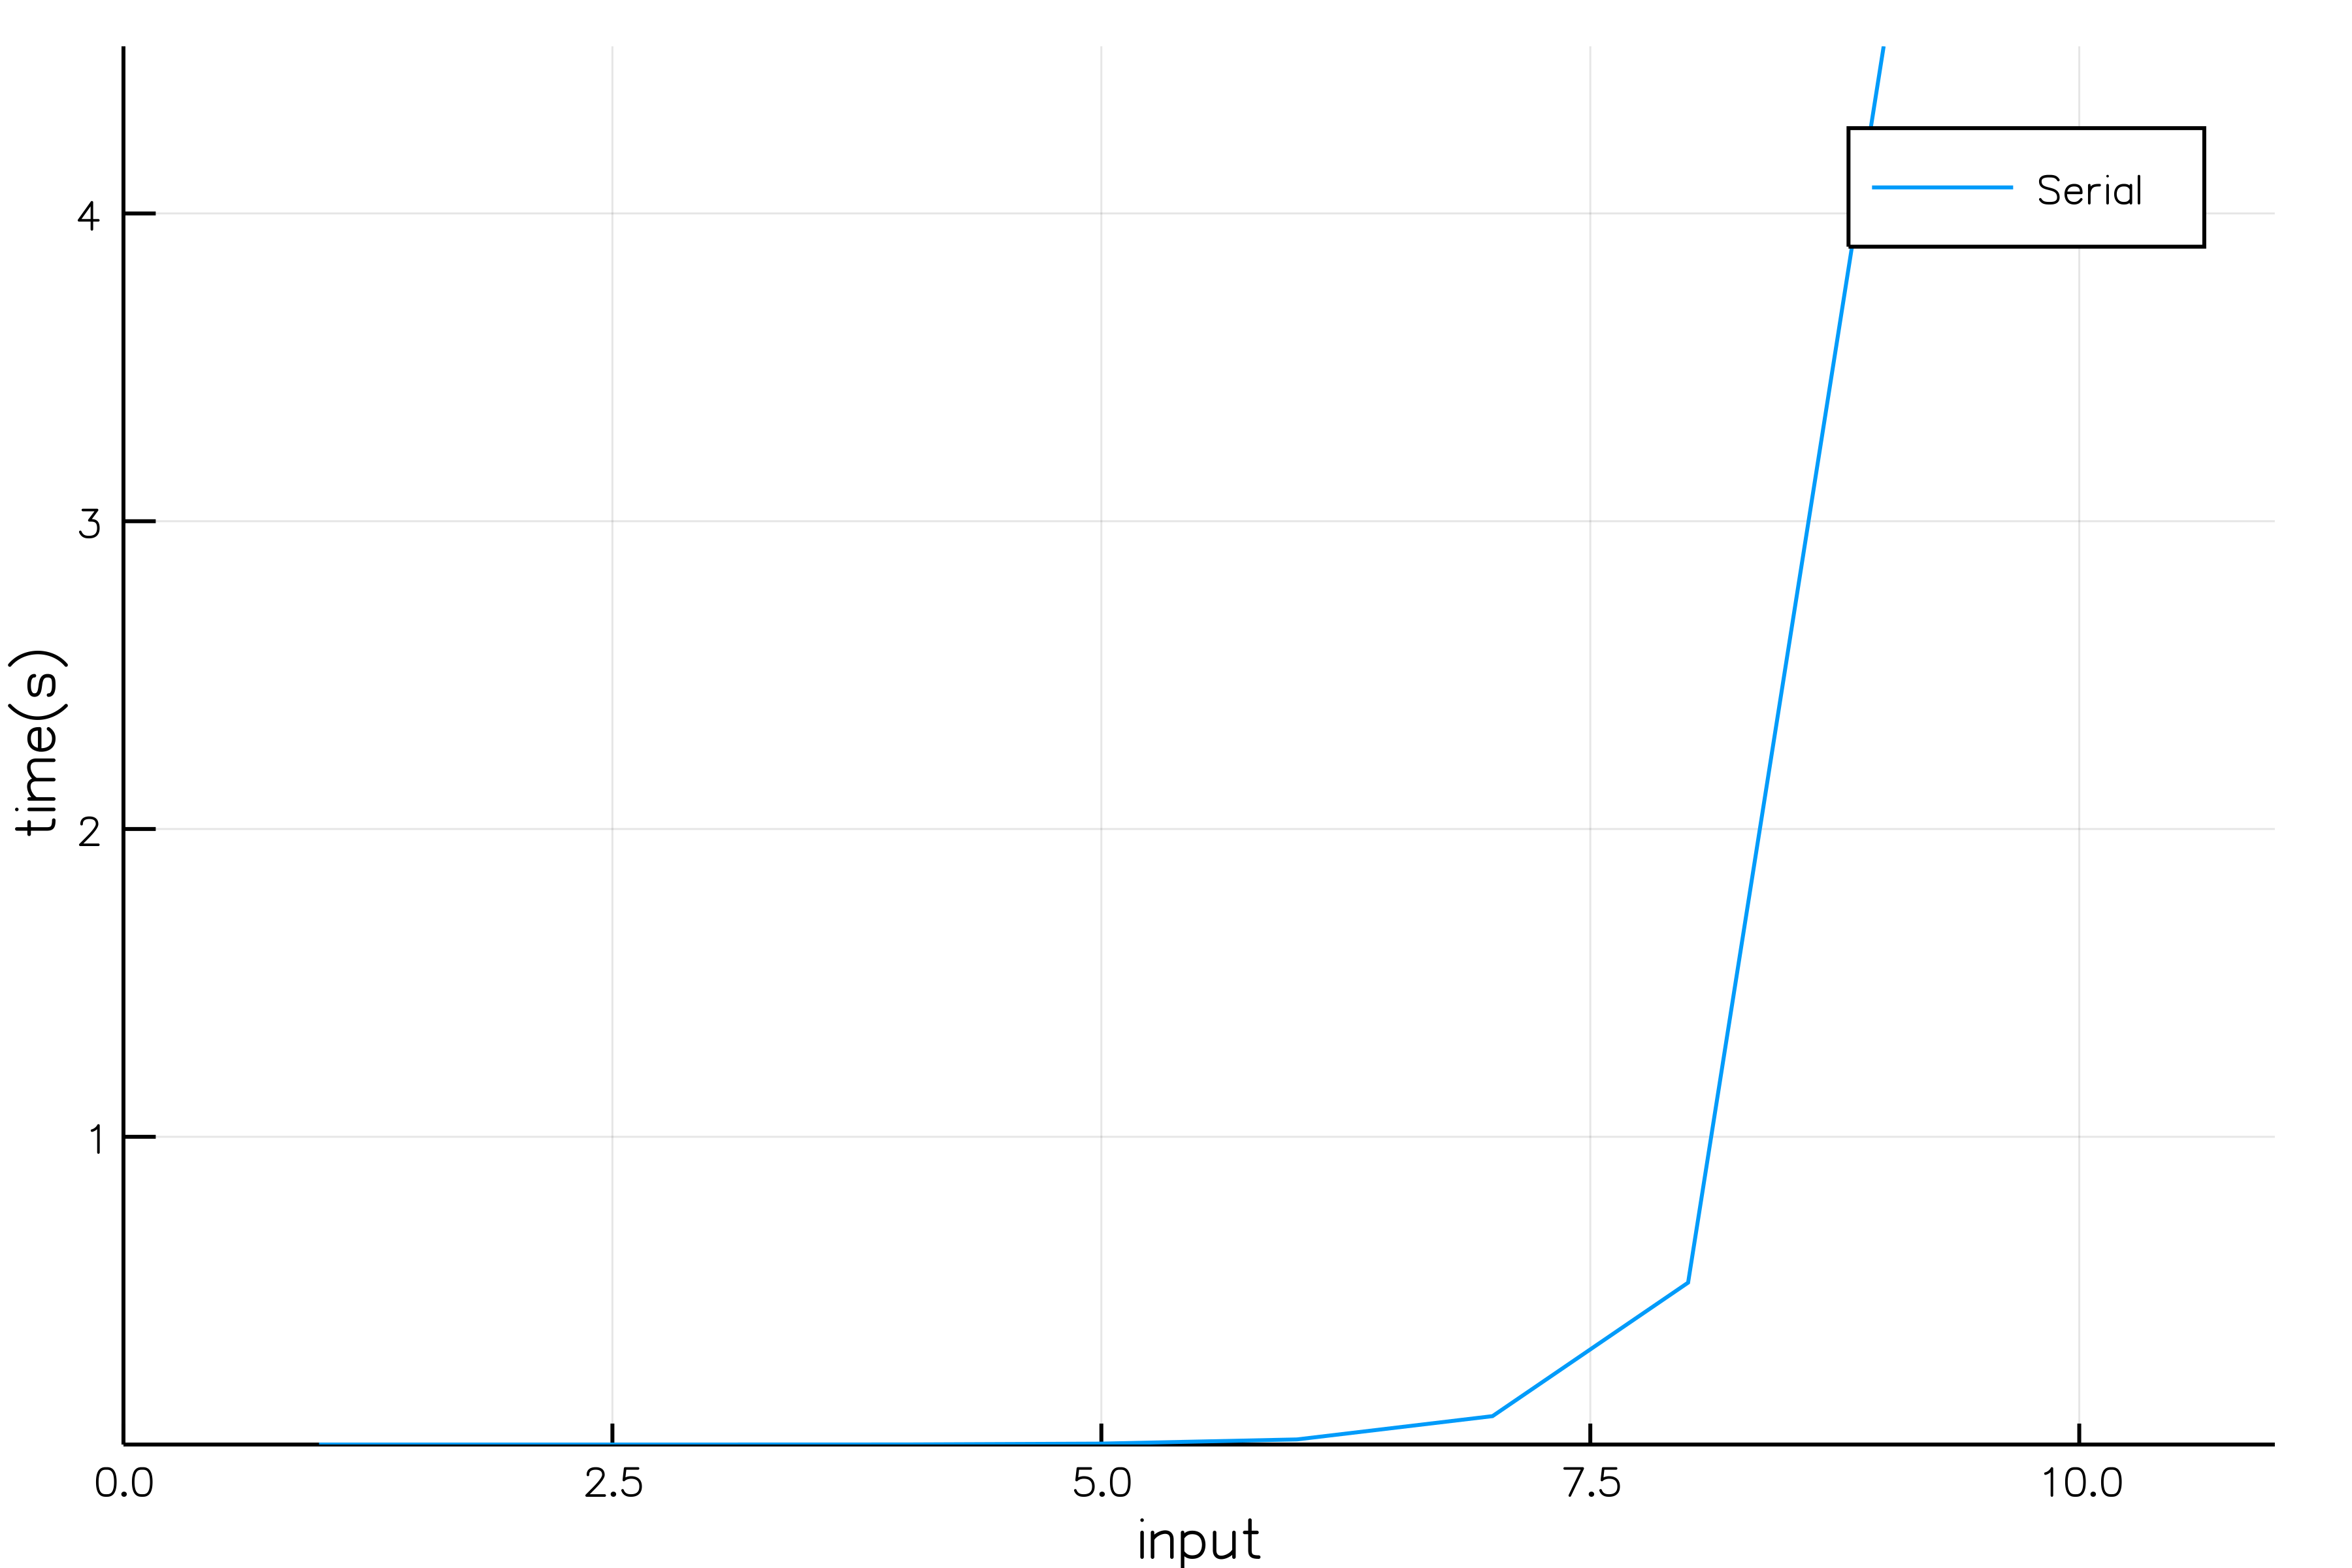
\includegraphics[scale=0.060]{boxSerial.png}
}
\subfloat[Parallel]{%
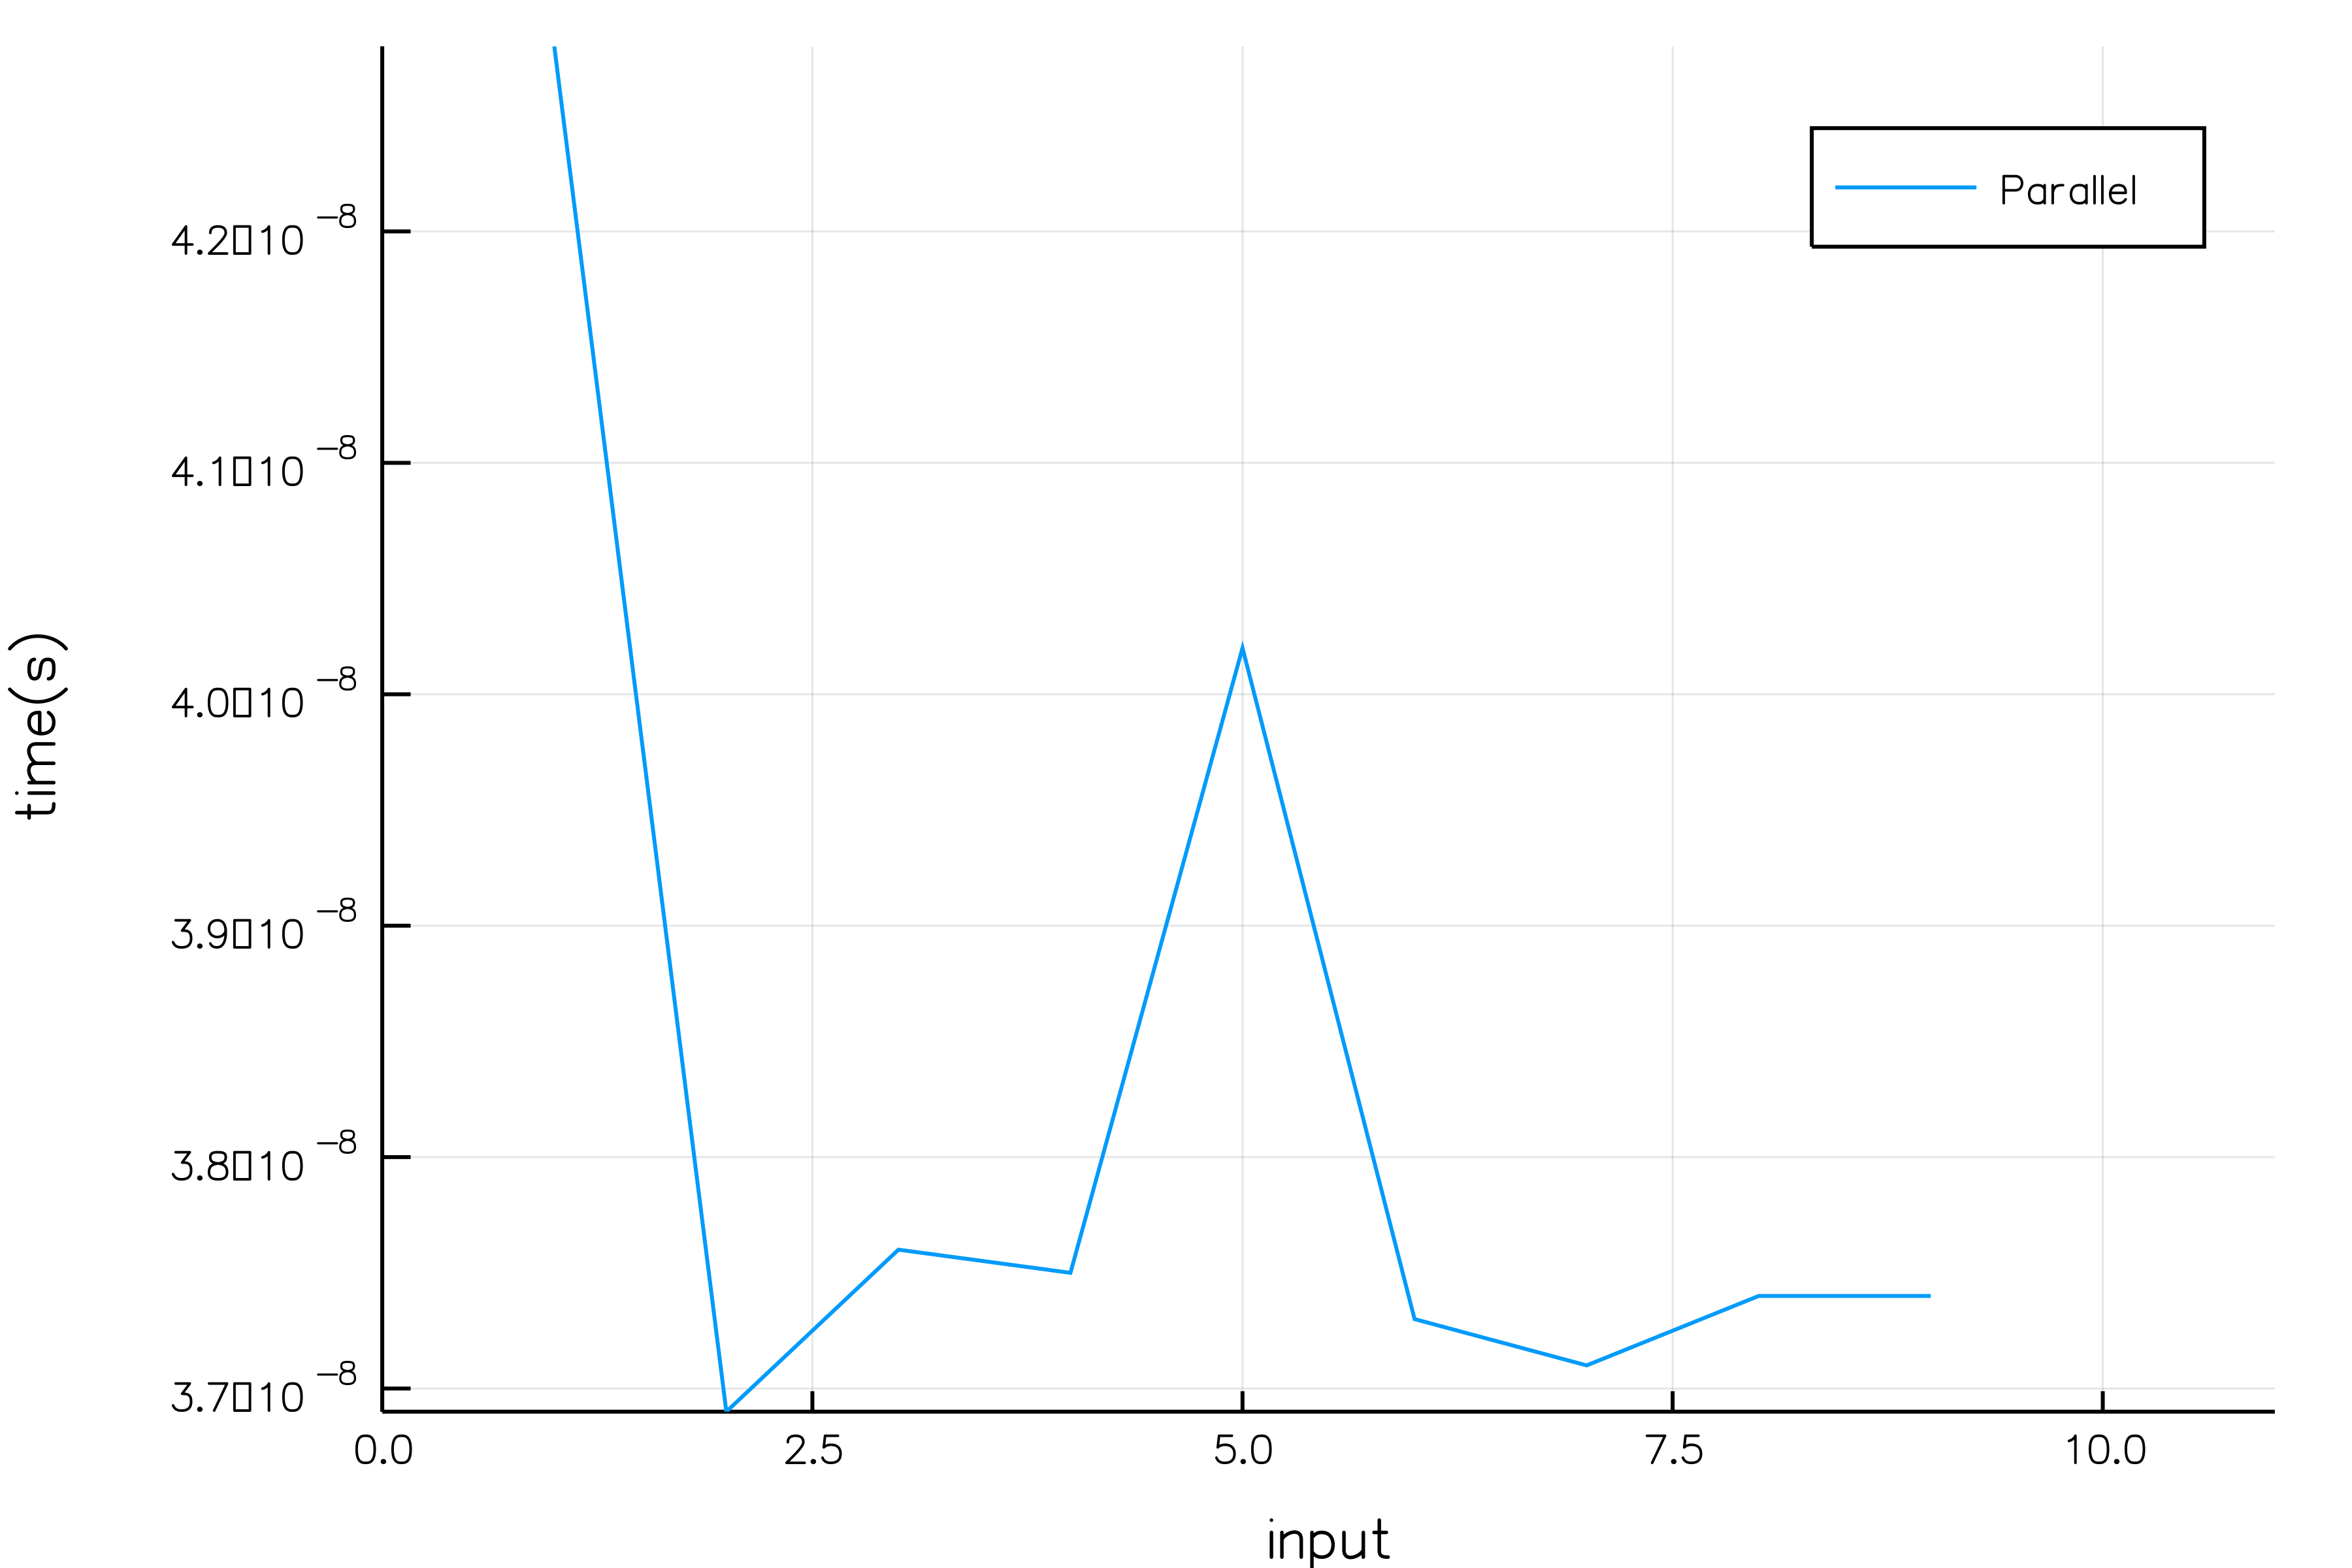
\includegraphics[scale=0.060]{boxParallel.png}
}
\caption{Execution time of function box}
\end{figure*}

\noindent \framebox[42em][c]{Compare}
\begin{Verbatim}[fontsize=\footnotesize]
plot([times,ptimes],xlabel="input",xlims=(0,length(ptimes)+2),ylabel="time(s)",
label=["Serial","Parallel"])
\end{Verbatim}
\begin{figure}[!h]
\centering
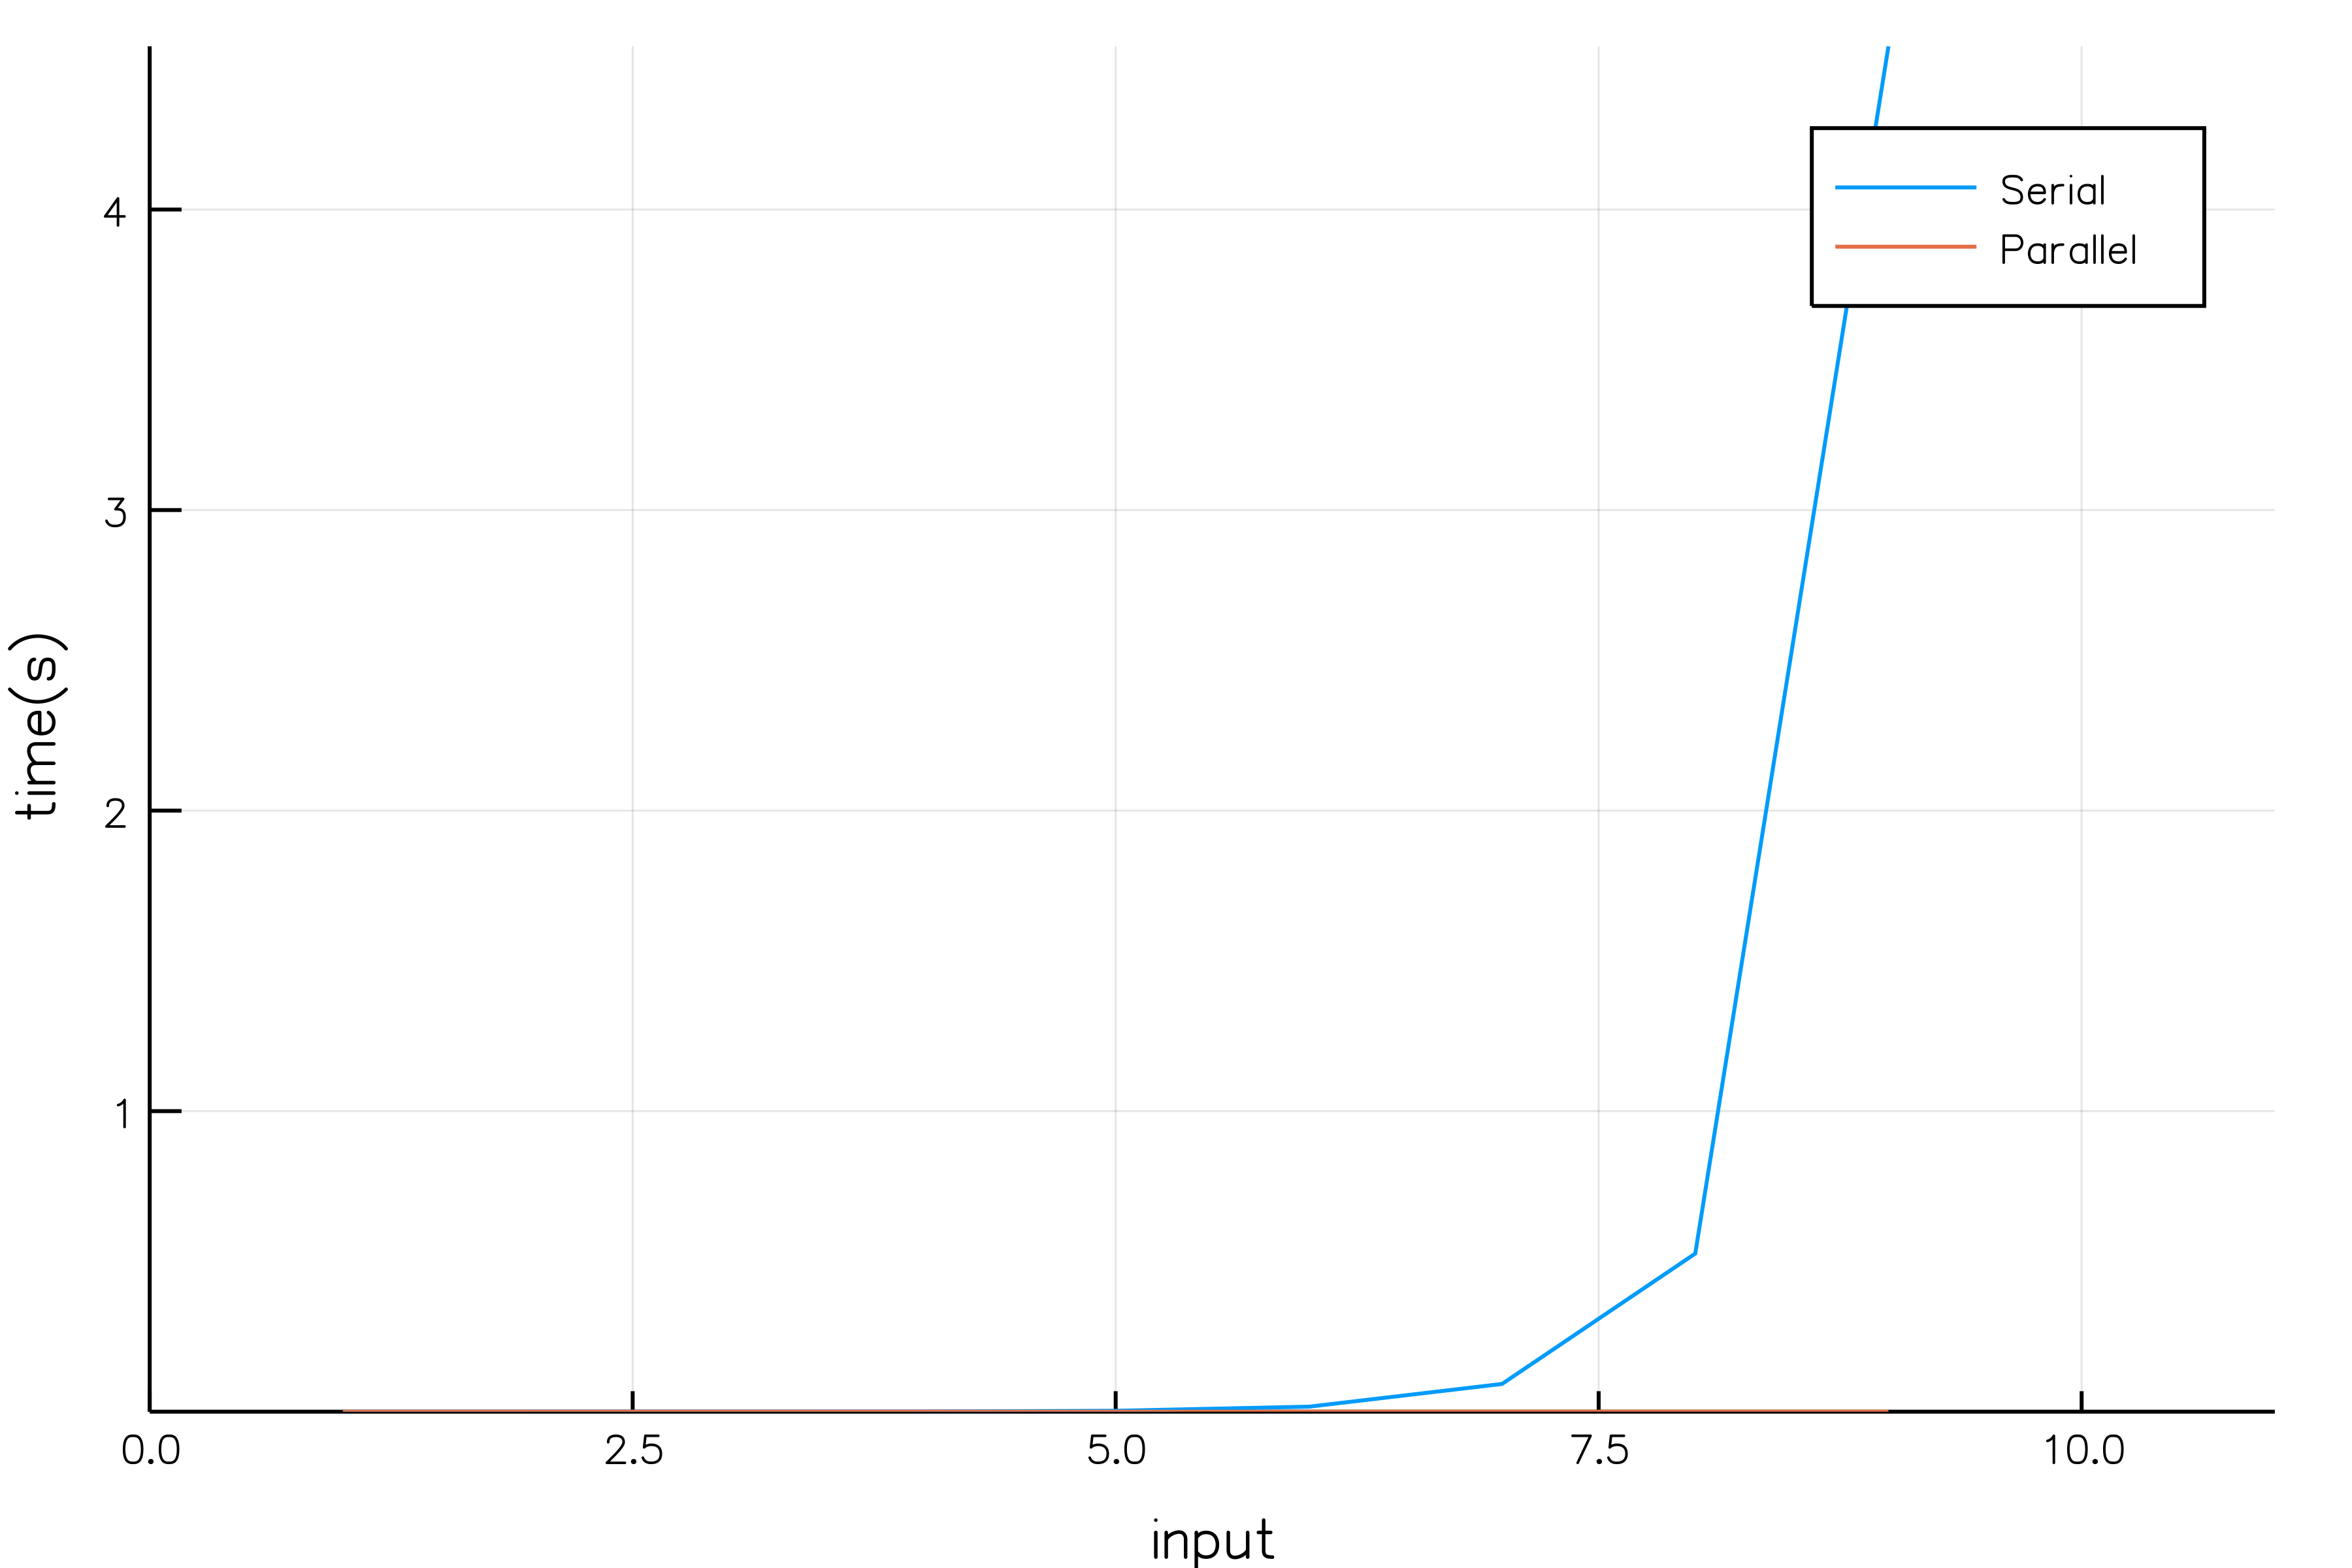
\includegraphics[scale=0.08]{boxC.png}
\caption{Compared execution time of function box}
\end{figure}
%__________________________________________________________________________________________________________________________
\newpage
\noindent\textbf{Execution time on Tesla}
\begin{Verbatim}[fontsize=\footnotesize]
input =[1,10,50,10^2,5*10^2,10^3,5*10^3,10^4,5*10^4,10^5,5*10^5,10^6]
function timeFstruct(f::Function,pf::Function,model,input)
  t=Array{Float64}(length(input))
  pt=Array{Float64}(length(input))
  for i in range(1,length(input))
    structo=addn2D(input[i],model)
    pstructo=pStruct(structo.body)
    f(structo)
    pf(pstructo)
    t[i]=@elapsed f(structo)
    pt[i]=@elapsed pf(pstructo)
  end
  return t,pt
end
y,yp=timeFstruct(box,pbox,square,input)
p=plot(y,xaxis="input",yaxis="time",xlims=(0,length(input)+1),ylims=(0,maximum(y)+0.5),
label=["Serial"],lw=2)
pp=plot(yp,xaxis="input",yaxis="time",xlims=(0,length(input)+1),ylims=(0,maximum(y)+0.5),
label=["Parallel"],lw=2)
\end{Verbatim}
\begin{figure*}[!h]
\centering
\subfloat[Serial]{%
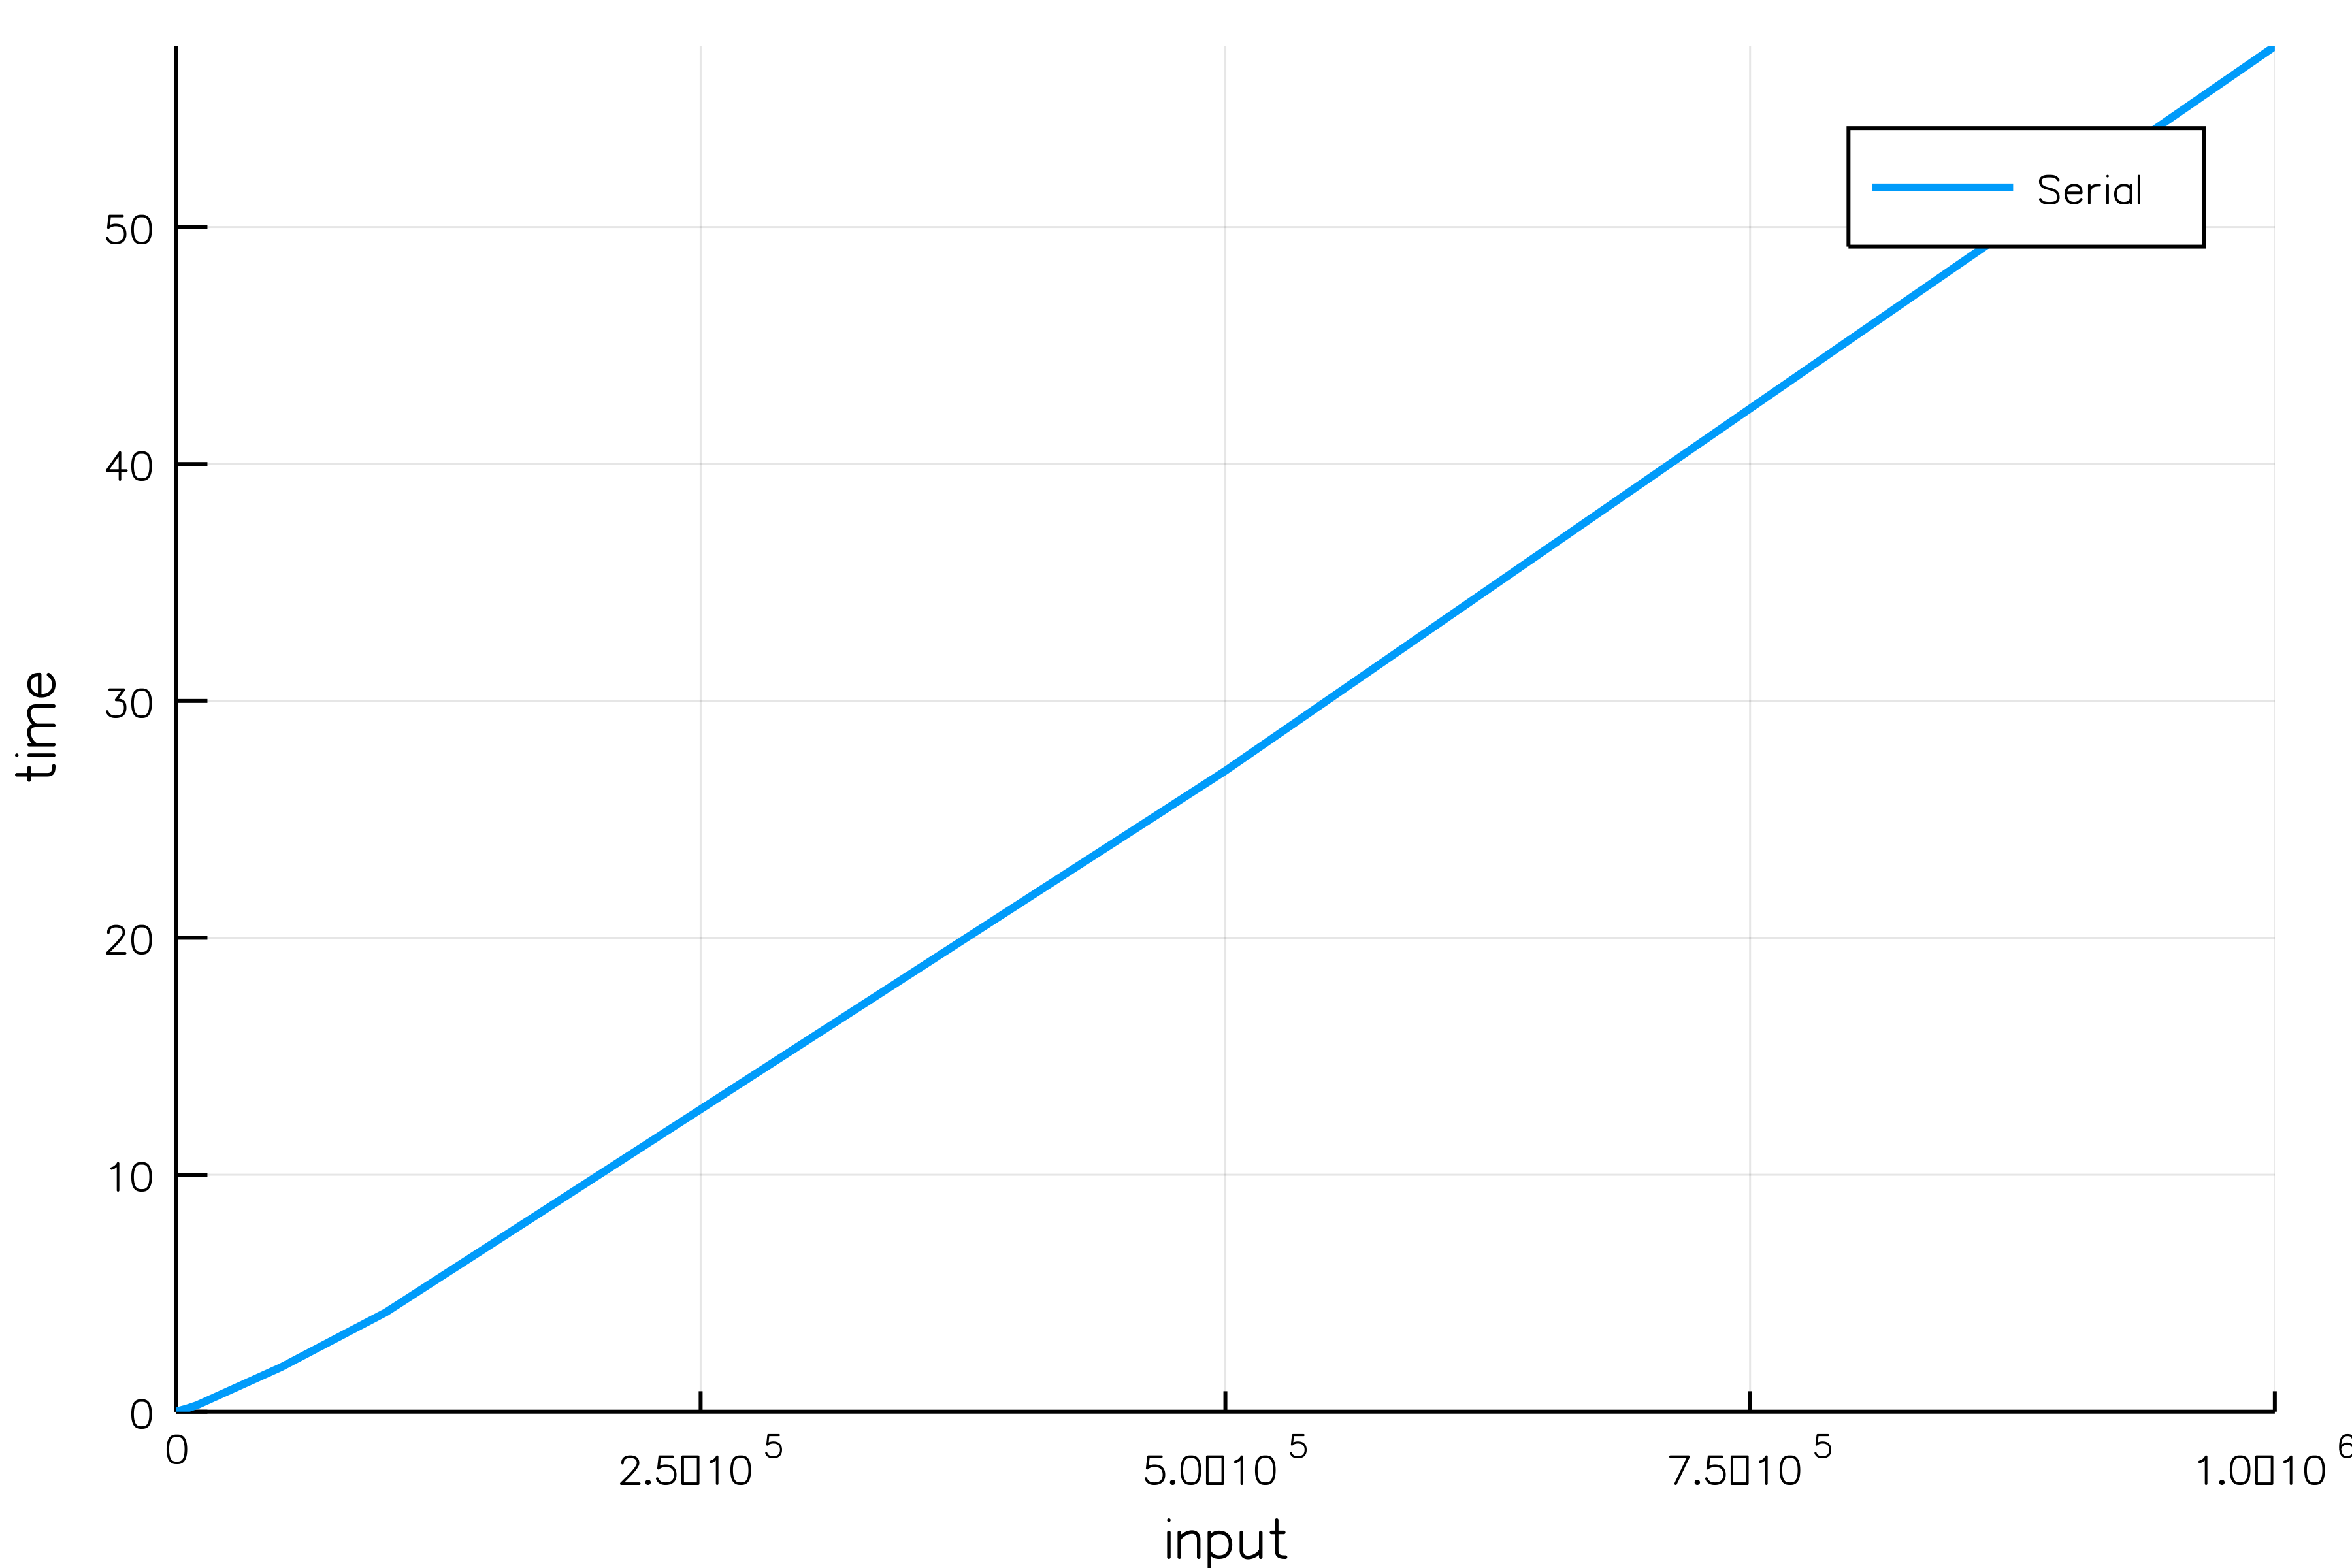
\includegraphics[scale=0.060]{box.png}
}
\subfloat[Parallel]{%
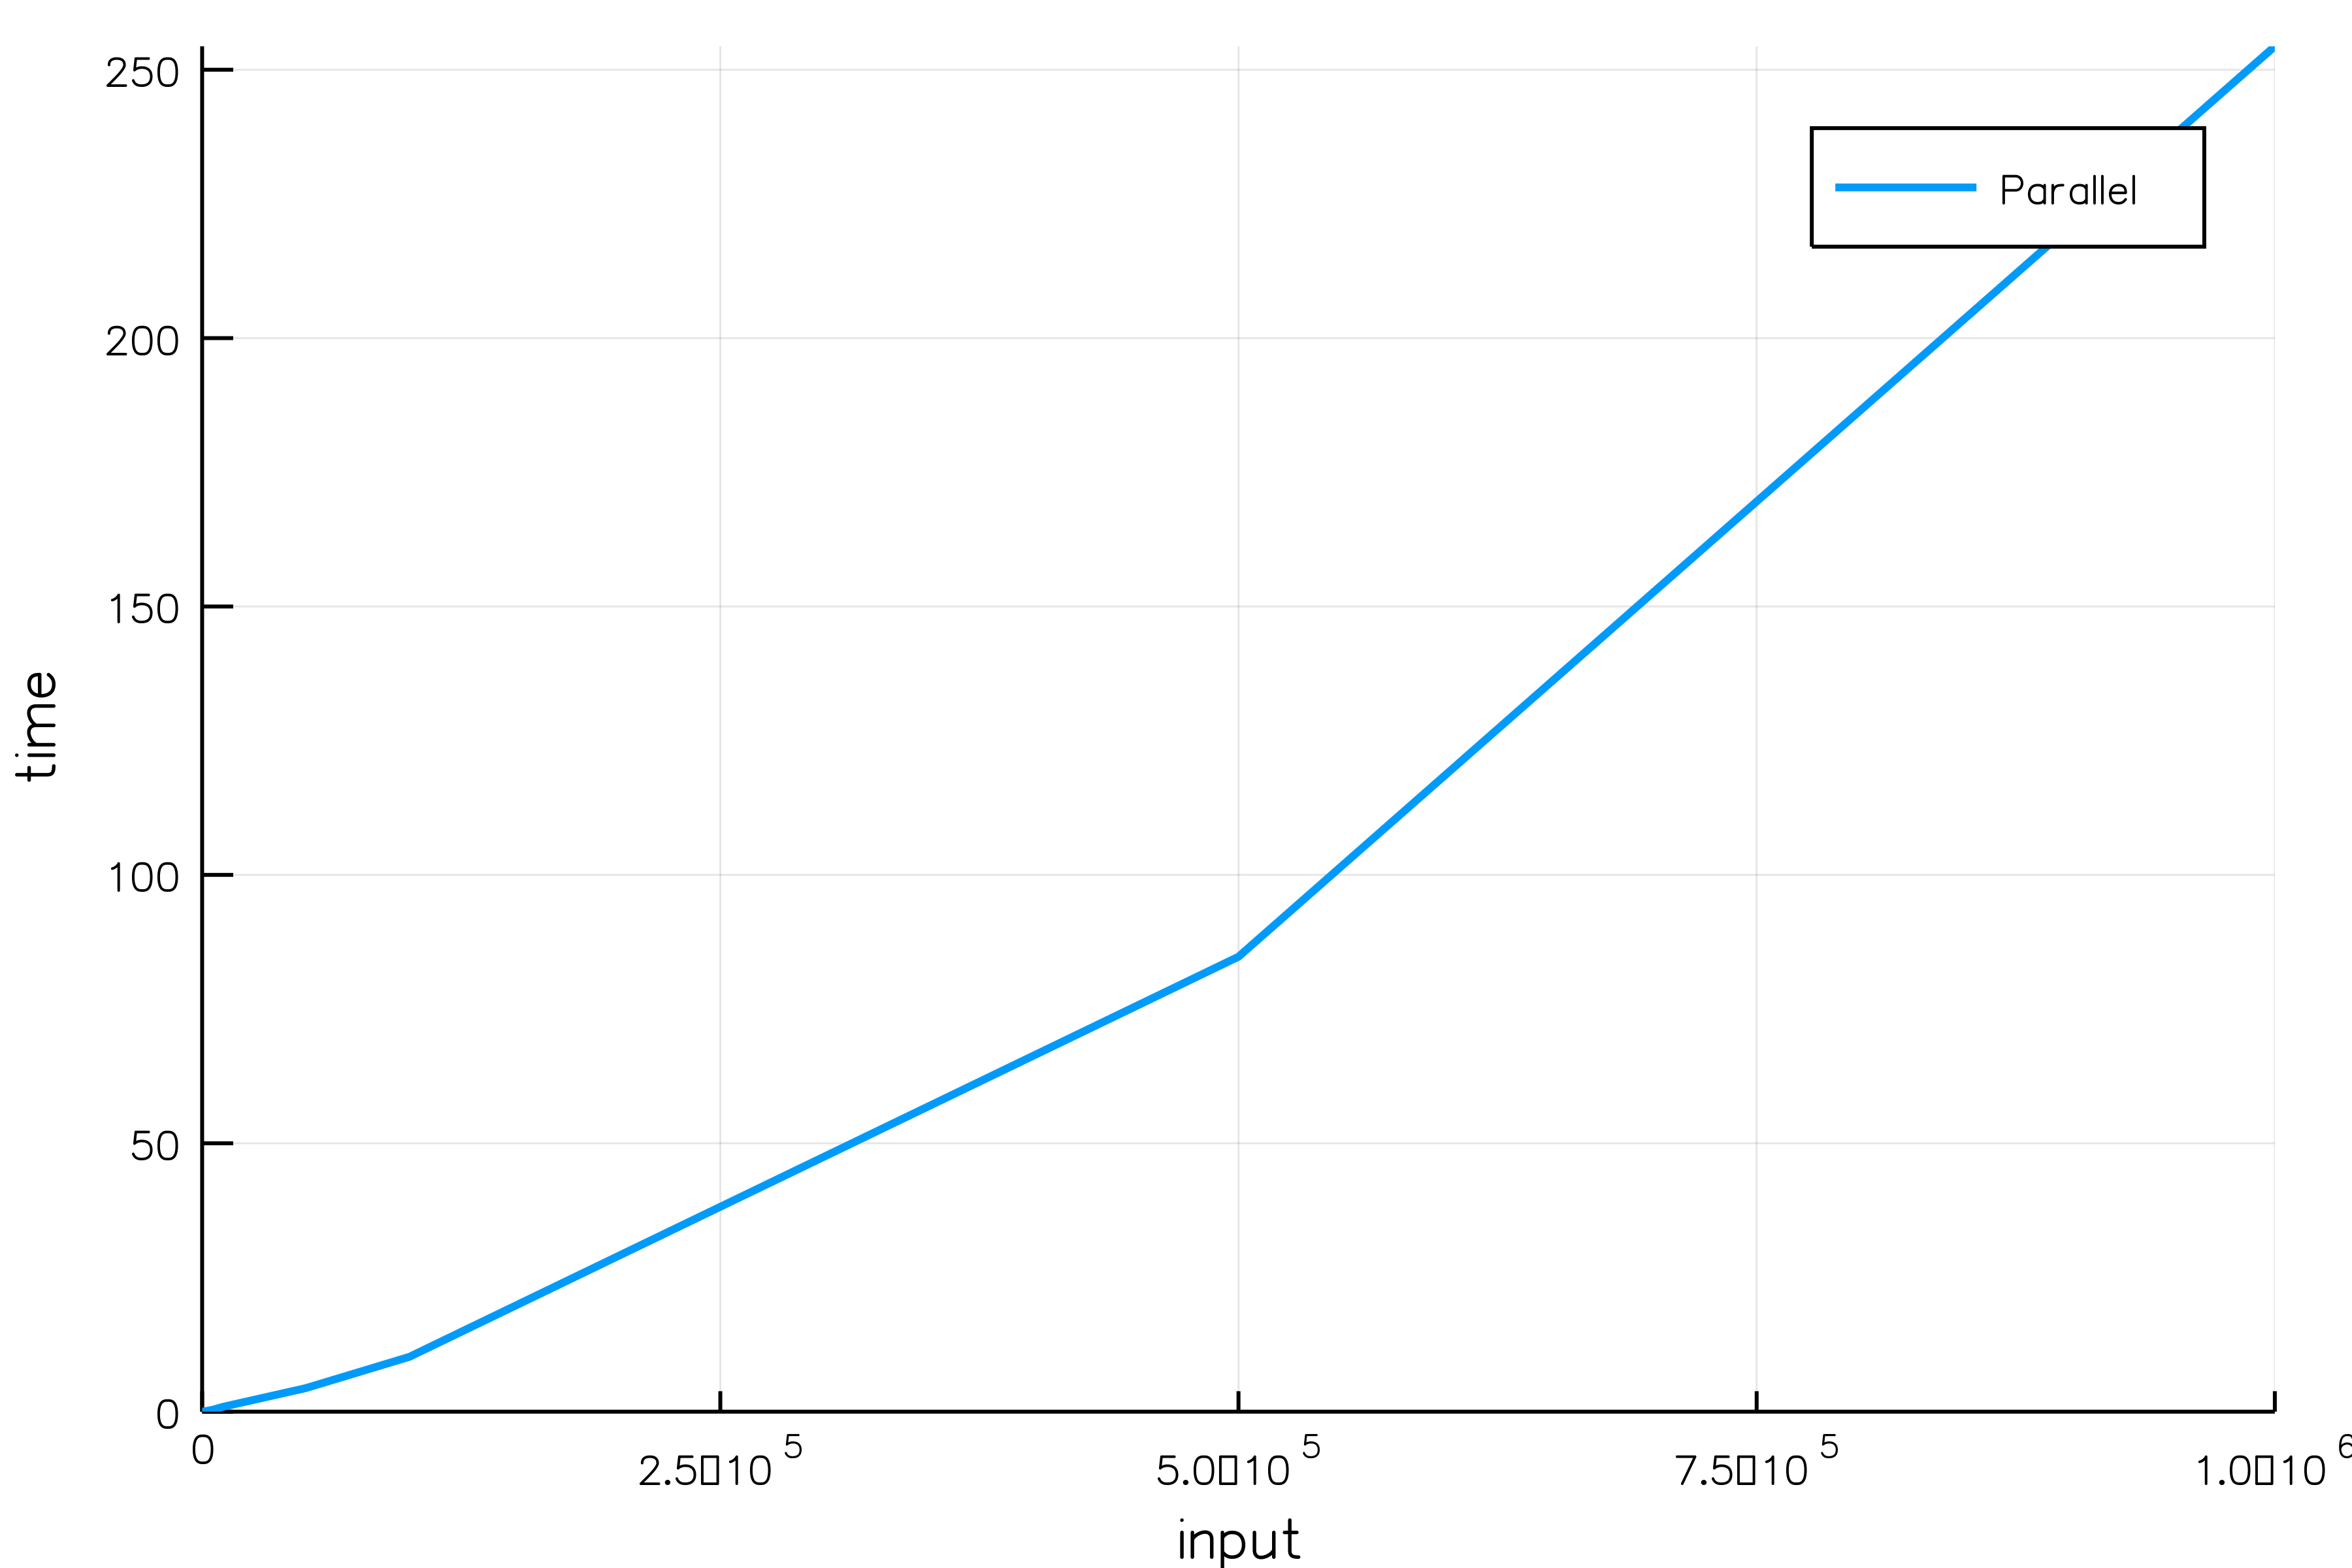
\includegraphics[scale=0.060]{pbox.png}
}
\caption{Execution time of function box on Tesla}
\end{figure*}
%__________________________________________________________________________________________________________________________
\newpage

\noindent \framebox[42em][c]{Compare}
\begin{Verbatim}[fontsize=\footnotesize]
yc=[y,yp]
pc=plot(y,xaxis="input",yaxis="time",xlims=(0,length(input)+1),ylims=(0,maximum(y)+0.5),
label=["Serial" "Parallel"],lw=2)
\end{Verbatim}
\begin{figure}[!h]
\centering
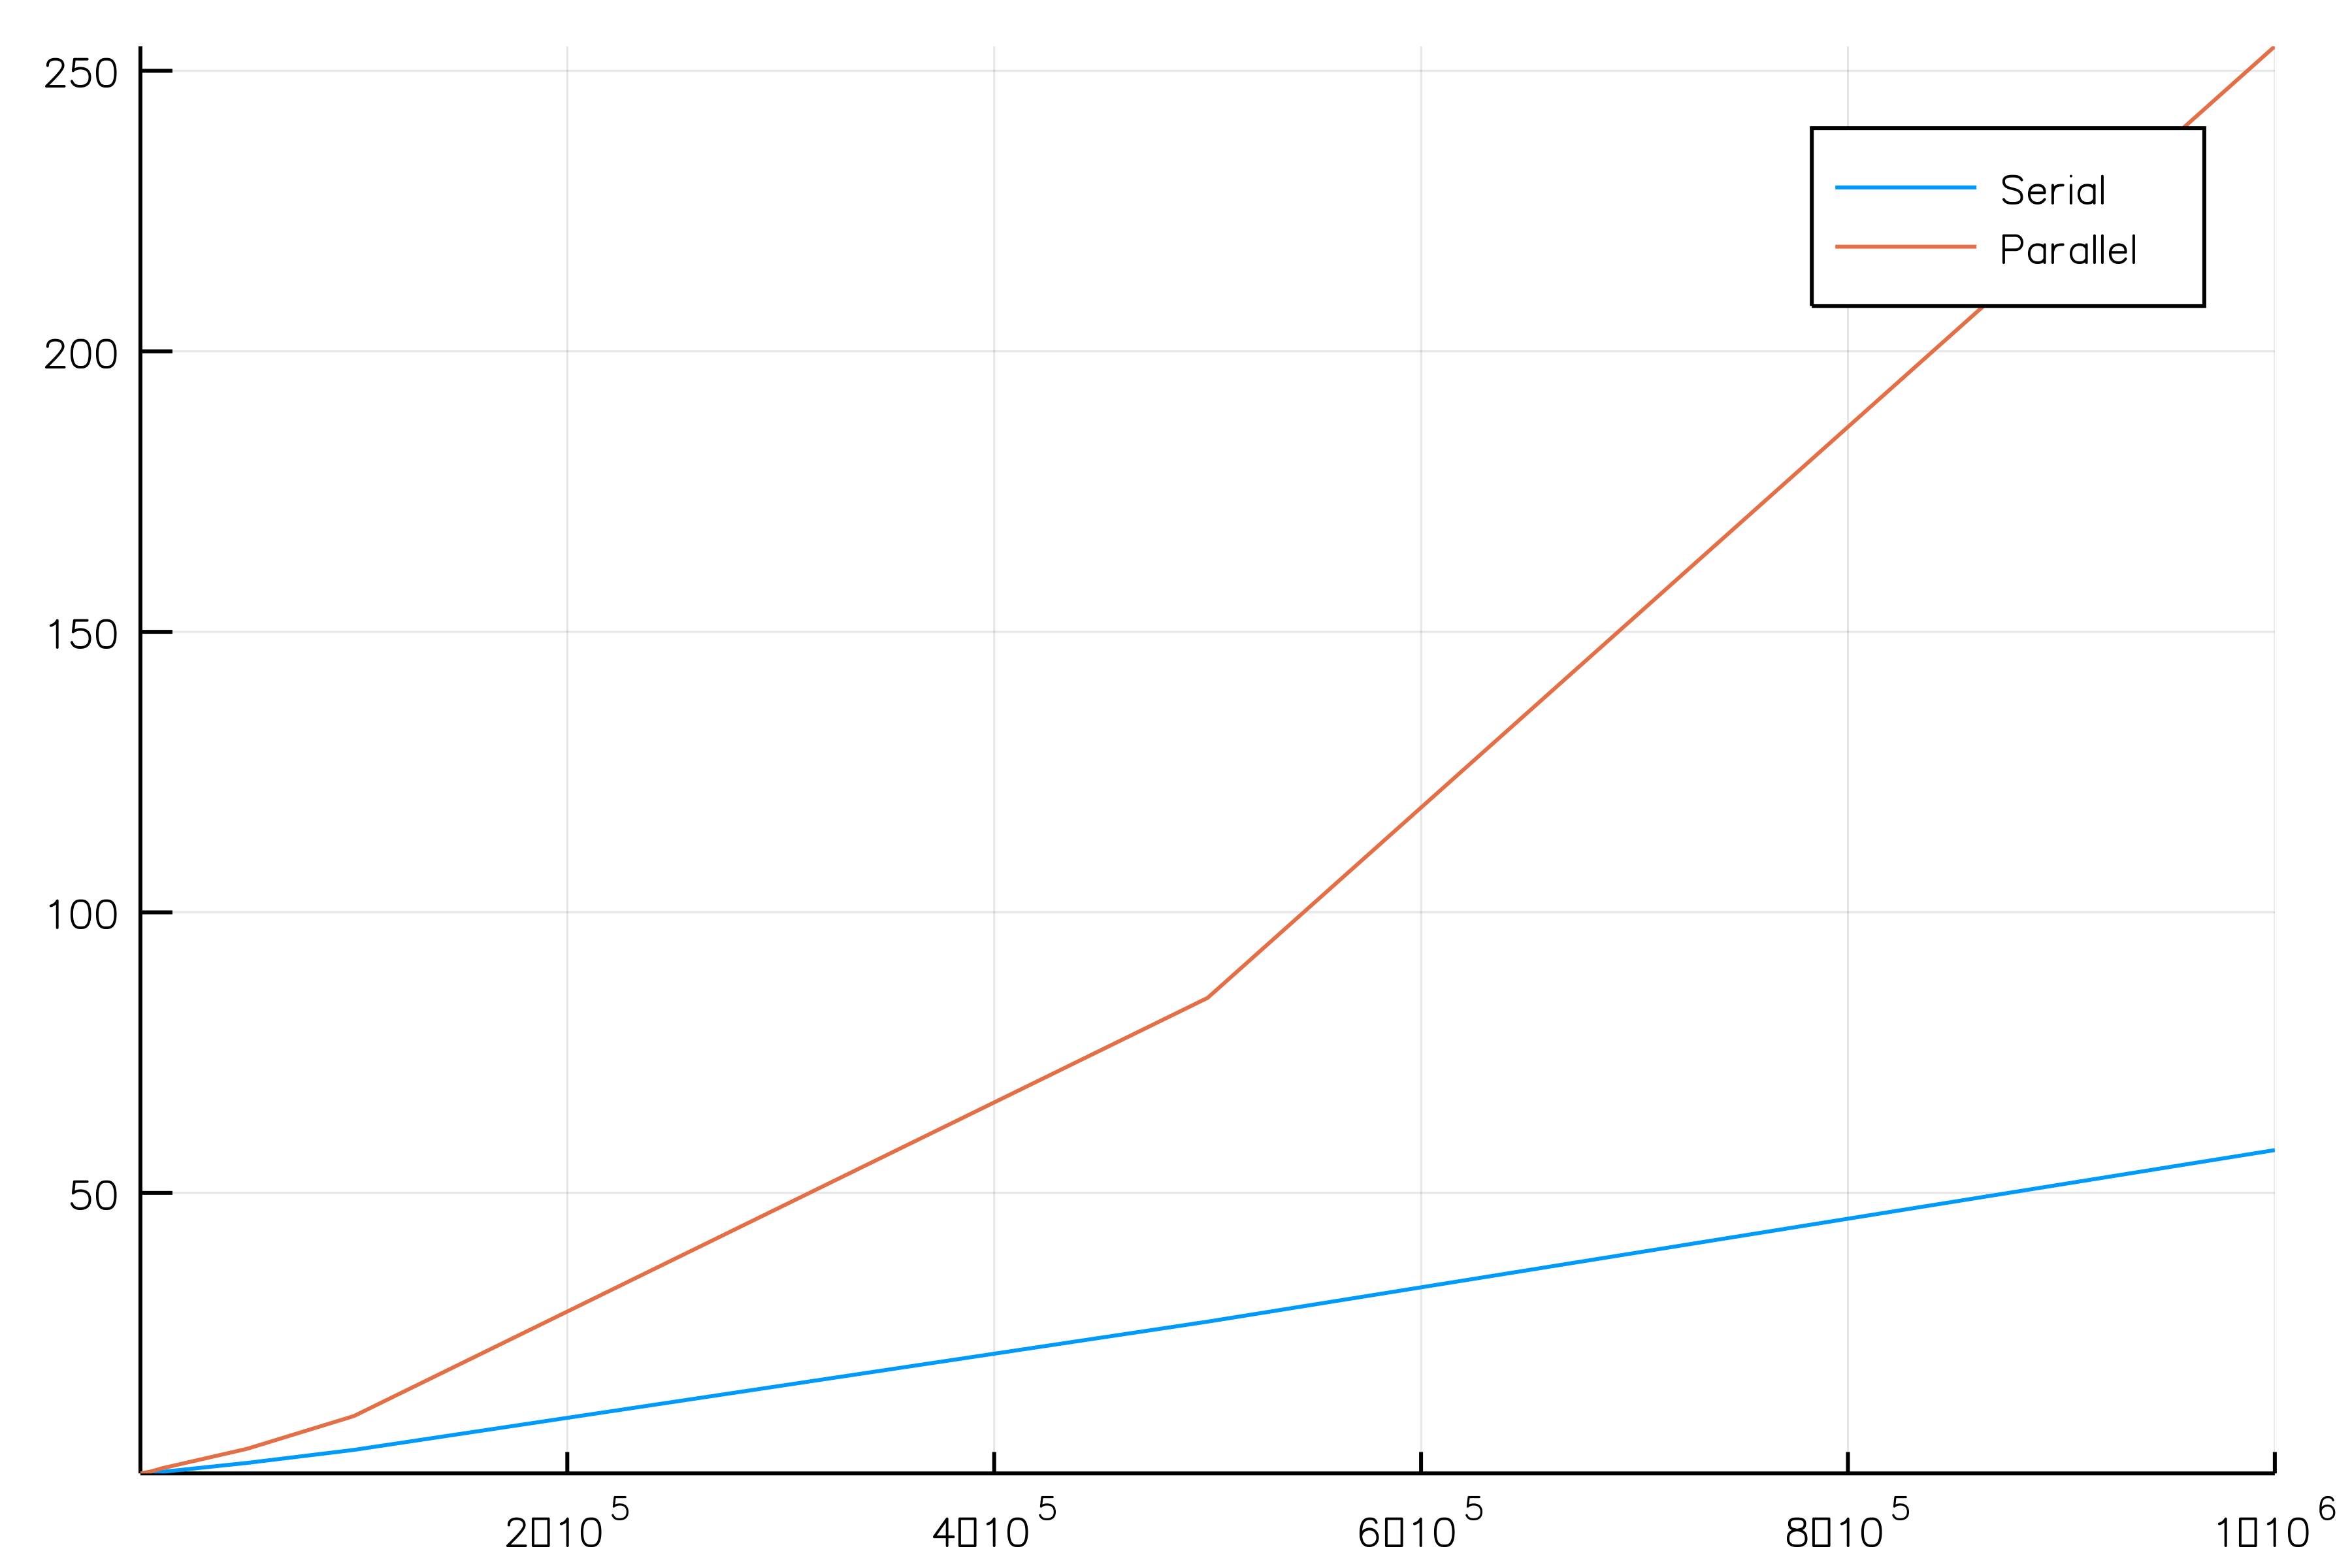
\includegraphics[scale=0.08]{compbox.png}
\caption{Compared Execution time of function box on Tesla}
\end{figure}

%__________________________________________________________________________________________________________________________________
\newpage

\subsection{traversal}
\subsubsection{Conversion}
\framebox[5em][c]{\textbf{\normalsize Python}}
\begin{Verbatim}[fontsize=\footnotesize]

def traversal(CTM, stack, obj, scene=[]):
  for i in range(len(obj)):
    if isinstance(obj[i],Model):
      scene += [larApply(CTM)(obj[i])]
    elif(isinstance(obj[i],tuple) or isinstance(obj[i],list)) and (len(obj[i]==2 orlen(obj[i])==3):
      scene += [larApply(CTM)(obj[i])]
    elif isinstance(obj[i],Mat): 
      CTM = scipy.dot(CTM, obj[i])
    elif isinstance(obj[i],Struct):
	stack.append(CTM)
	traversal(CTM, stack, obj[i], scene)
	CTM = stack.pop()
  return scene
\end{Verbatim}
\framebox[5em][c]{\textbf{\normalsize Julia}}
\begin{Verbatim}[fontsize=\footnotesize]

function traversal(CTM,stack,obj,scene=[])
  for i in range(1,len(obj))
    if isa(obj.body[i],Matrix)
      CTM = CTM * obj.body[i]
    elseif (isa(obj.body[i],Tuple)||isa(obj.body[i],Array))&&
    (length(obj.body[i])==2||length(obj.body[i])==3)
      l=larApply(CTM)(obj.body[i])
      push!(scene,l)
    elseif isa(obj.body[i],Struct)
      push!(stack,CTM)
      traversal(CTM,stack,obj.body[i],scene)
      CTM = pop!(stack)
    end
  end
  return scene
end

\end{Verbatim}
\subsubsection{Parallelization}
\begin{Verbatim}[fontsize=\footnotesize]

@everywhere function ptraversal(CTM,stack,obj,scene=[])
  @sync for i in range(1,len(obj))
    if isa(obj.body[i],Matrix)
      CTM = CTM*obj.body[i]
    elseif (isa(obj.body[i],Tuple)||isa(obj.body[i],Array))&&
    (length(obj.body[i])==2||length(obj.body[i])==3)
      l=plarApply(CTM)(obj.body[i])
      push!(scene,l)
    elseif isa(obj.body[i],pStruct)
      push!(stack,CTM)
      ptraversal(CTM,stack,obj.body[i],scene)
      CTM = pop!(stack)
    end
  end
  return scene
end

\end{Verbatim}
\subsubsection{Unit-Test}
These tests can be runned after the definition of the Struct type on the section \ref{Struct}
\vspace{25px}

\noindent \framebox[42em][c]{Serial Tests}
\begin{Verbatim}[fontsize=\footnotesize]

@testset "traversal Tests" begin
   square=([[0, 0], [0, 1], [1, 0], [1, 1]], [[0, 1, 2, 3]])
   
   @everywhere structure=Struct([square])
   @everywhere d=checkStruct(structure.body)
   @test length(traversal(eye(d+1),[],structure,[]))==length(structure.body)
   @test typeof(traversal(eye(d+1),[],structure,[]))==Array{Any,1}
end
\end{Verbatim}

\noindent \framebox[42em][c]{Parallel Tests}
\begin{Verbatim}[fontsize=\footnotesize]
square=([[0, 0], [0, 1], [1, 0], [1, 1]], [[0, 1, 2, 3]])
structure=pStruct([square])
d=pcheckStruct(structure.body)

@testset "ptraversal Tests" begin
  @test length(ptraversal(eye(d+1),[],structure,[]))==length(structure.body)
  @test typeof(ptraversal(eye(d+1),[],structure,[]))==Array{Any,1}
end
\end{Verbatim}
\subsubsection{Results}
\textbf{Execution time on PC}
\begin{Verbatim}[fontsize=\footnotesize]
times=[]
ptimes=[]
input=[]
dim=[]

for i in range(1,length(l)-1)
  push!(input,Struct([repeat([l[i]],outer=i)...]))
end

append!(dim,checkStruct(input[i].body) for i in range(1,length(input)))

for i in range(1,length(input))
  args=(eye(dim[i]+1),[],input[i],[])
  append!(times,Time(traversal,(args...)))
end
for i in range(1,length(input))
  args=(eye(dim[i]+1),[],input[i],[])
  append!(ptimes,Time(ptraversal,(args...)))
end

plot(times,xlabel="input",xlims=(0,length(times)+2),ylabel="time(s)",label=["Serial"])
plot(ptimes,xlabel="input",xlims=(0,length(times)+2),ylabel="time(s)",label=["Parallel"])

\end{Verbatim}

\begin{figure*}[!h]
\centering
\subfloat[Serial]{%
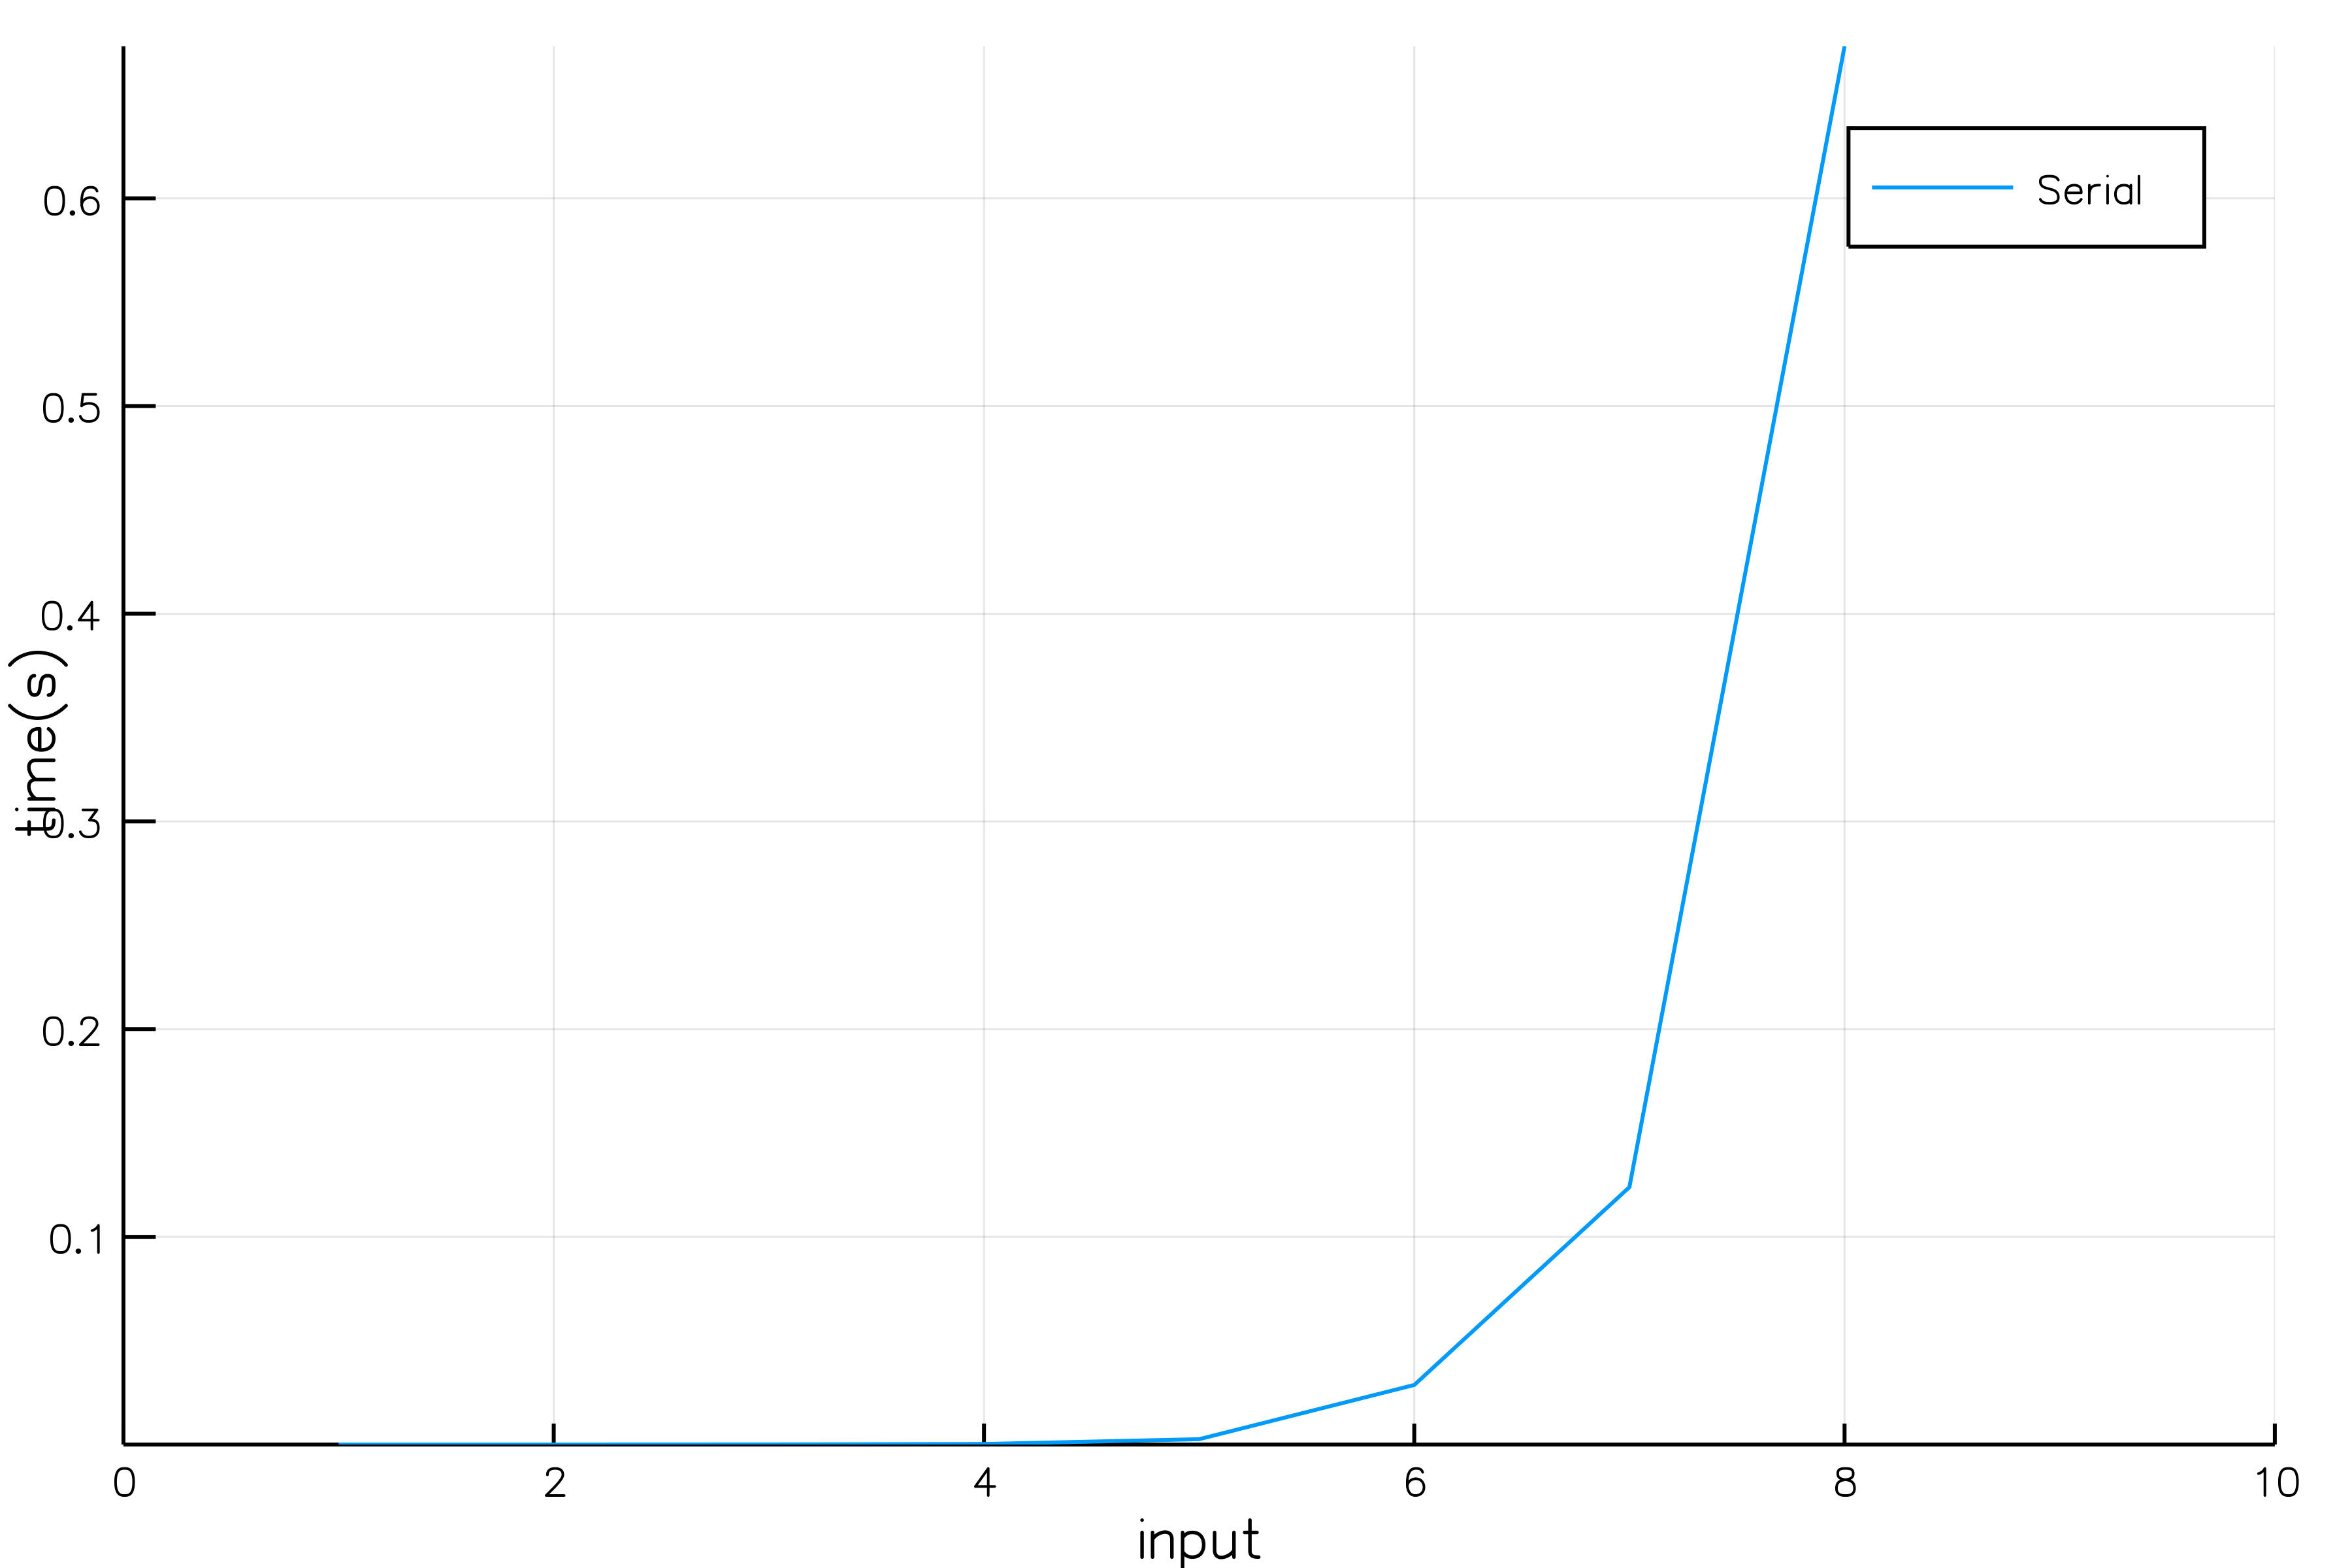
\includegraphics[scale=0.060]{traversalSerial.png}
}
\subfloat[Parallel]{%
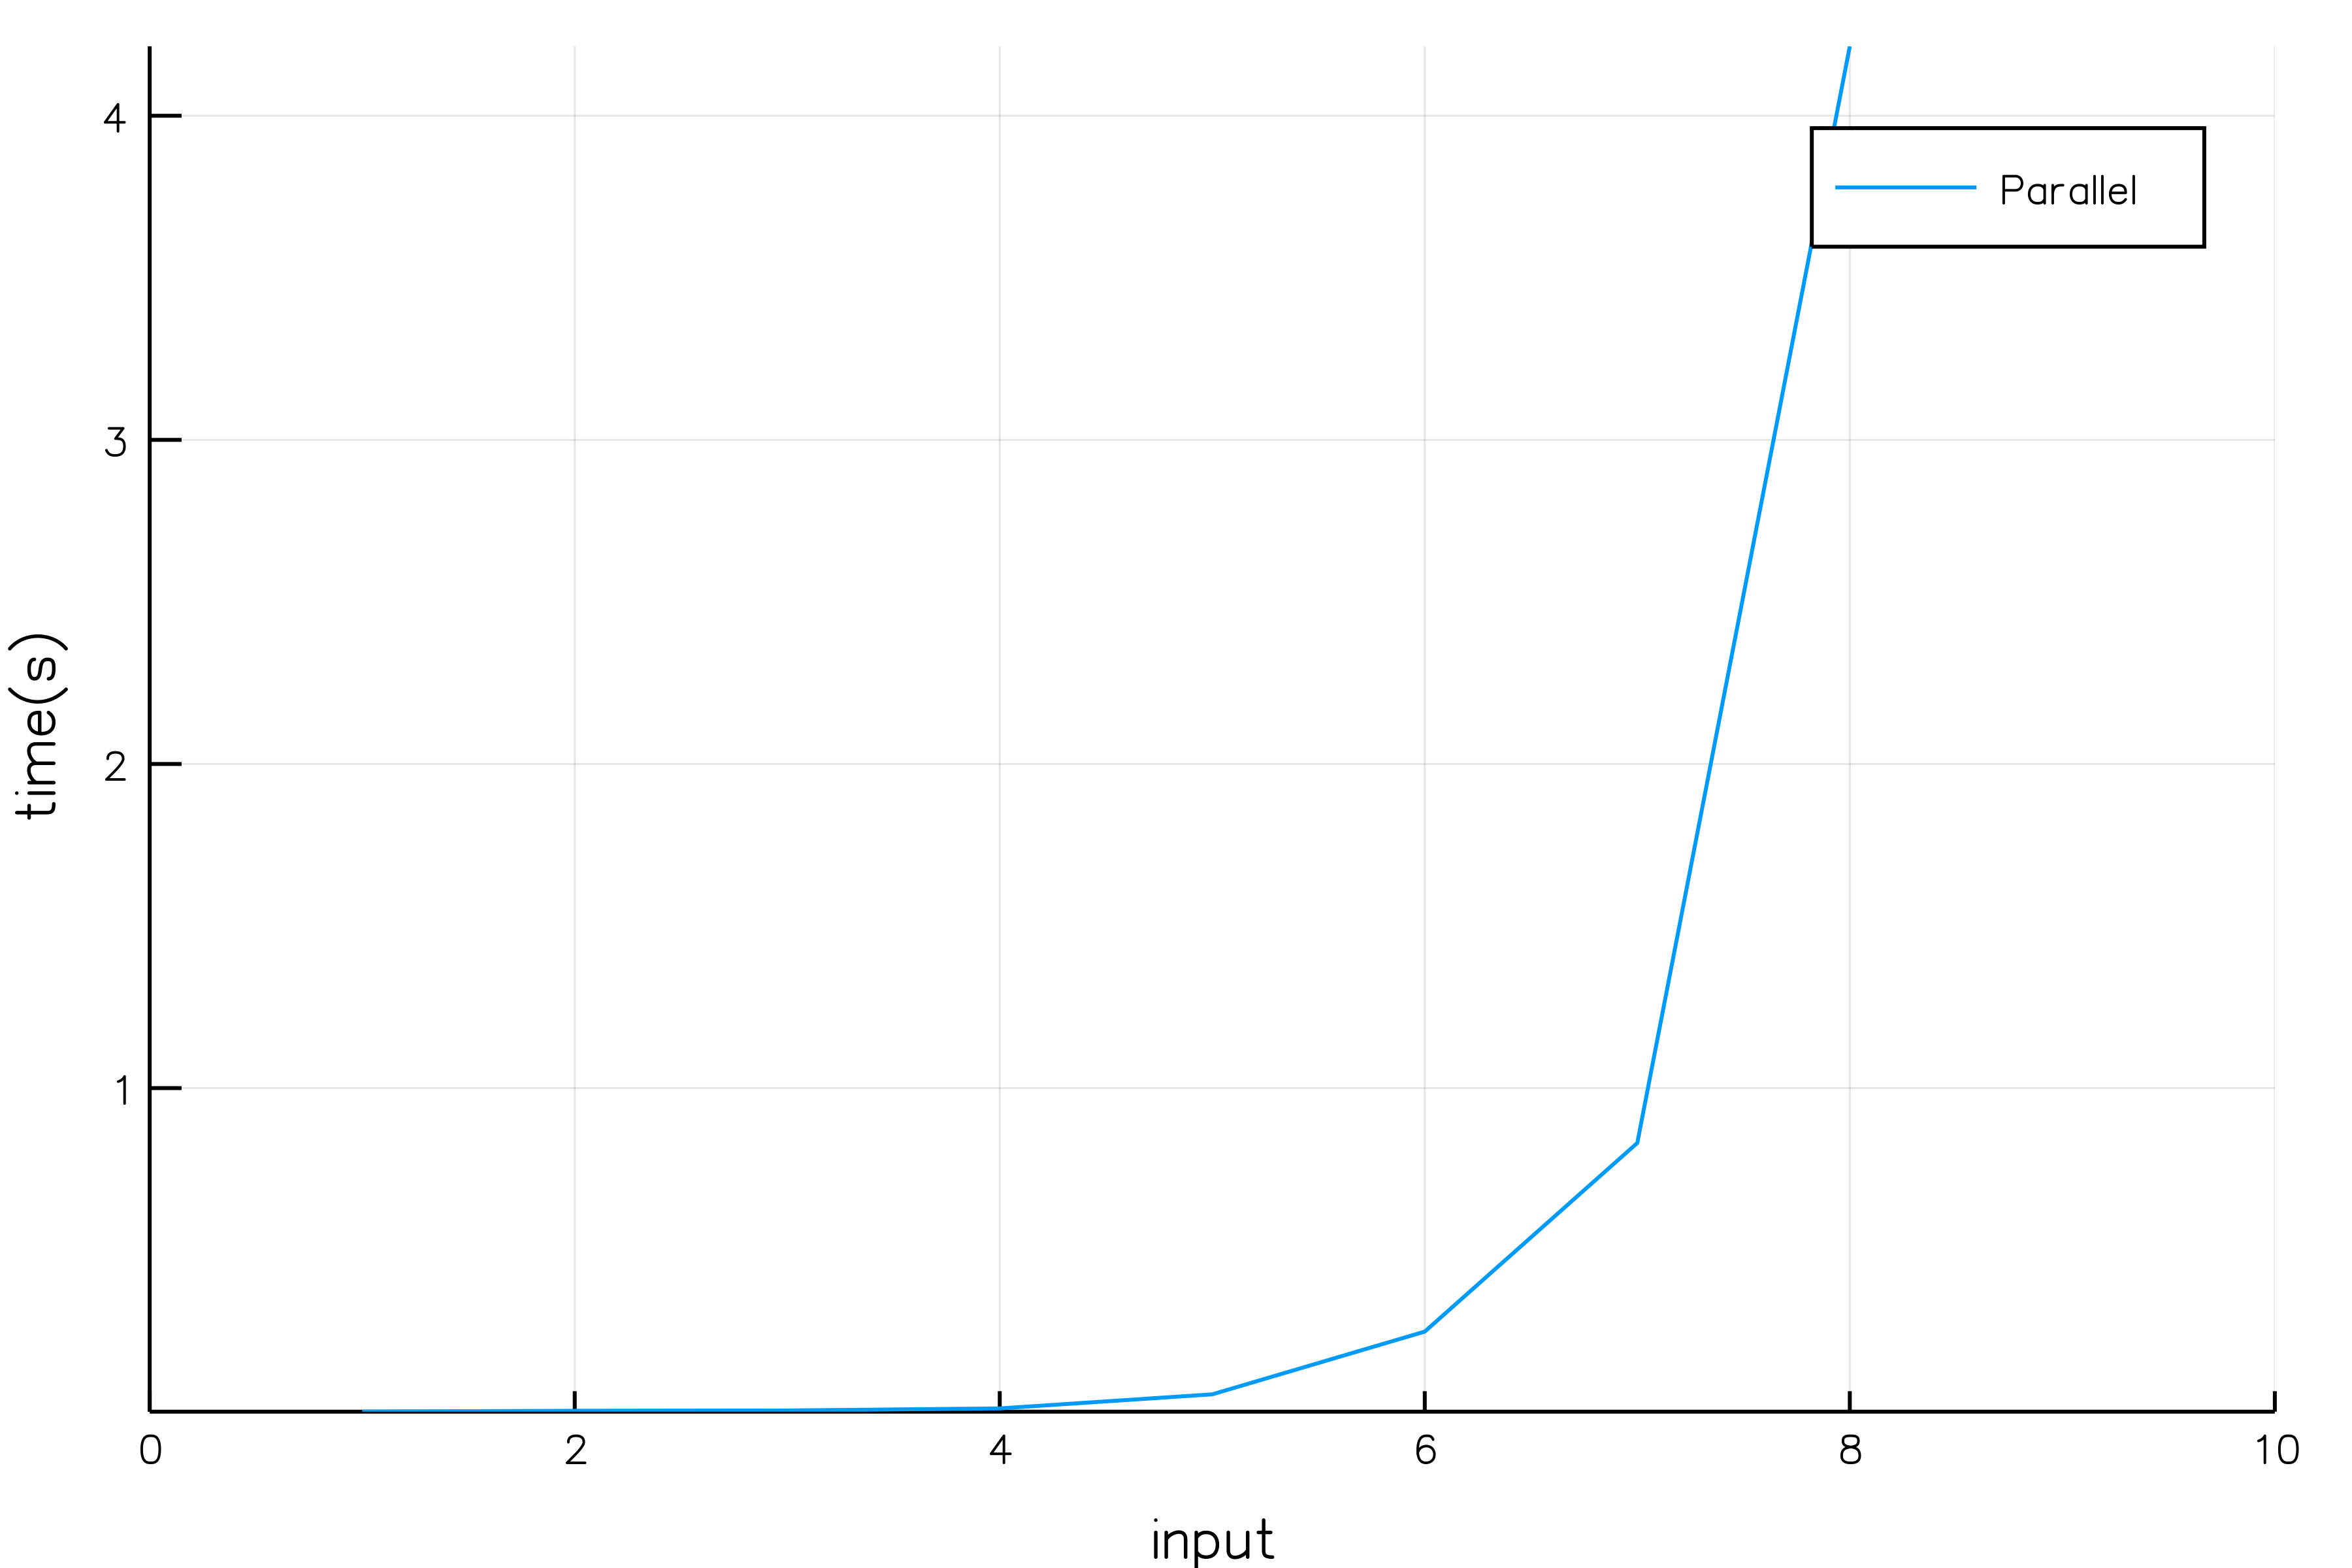
\includegraphics[scale=0.060]{traversalParallel.png}
}
\caption{Execution time of function traversal}
\end{figure*}

%__________________________________________________________________________________________________________________________
\newpage

\noindent \framebox[42em][c]{Compare}
\begin{Verbatim}[fontsize=\footnotesize]

plot([times,ptimes],xlabel="input",xlims=(0,length(ptimes)+2),ylabel="time(s)",
label=["Serial","Parallel"])

\end{Verbatim}

\begin{figure}[!h]
\centering
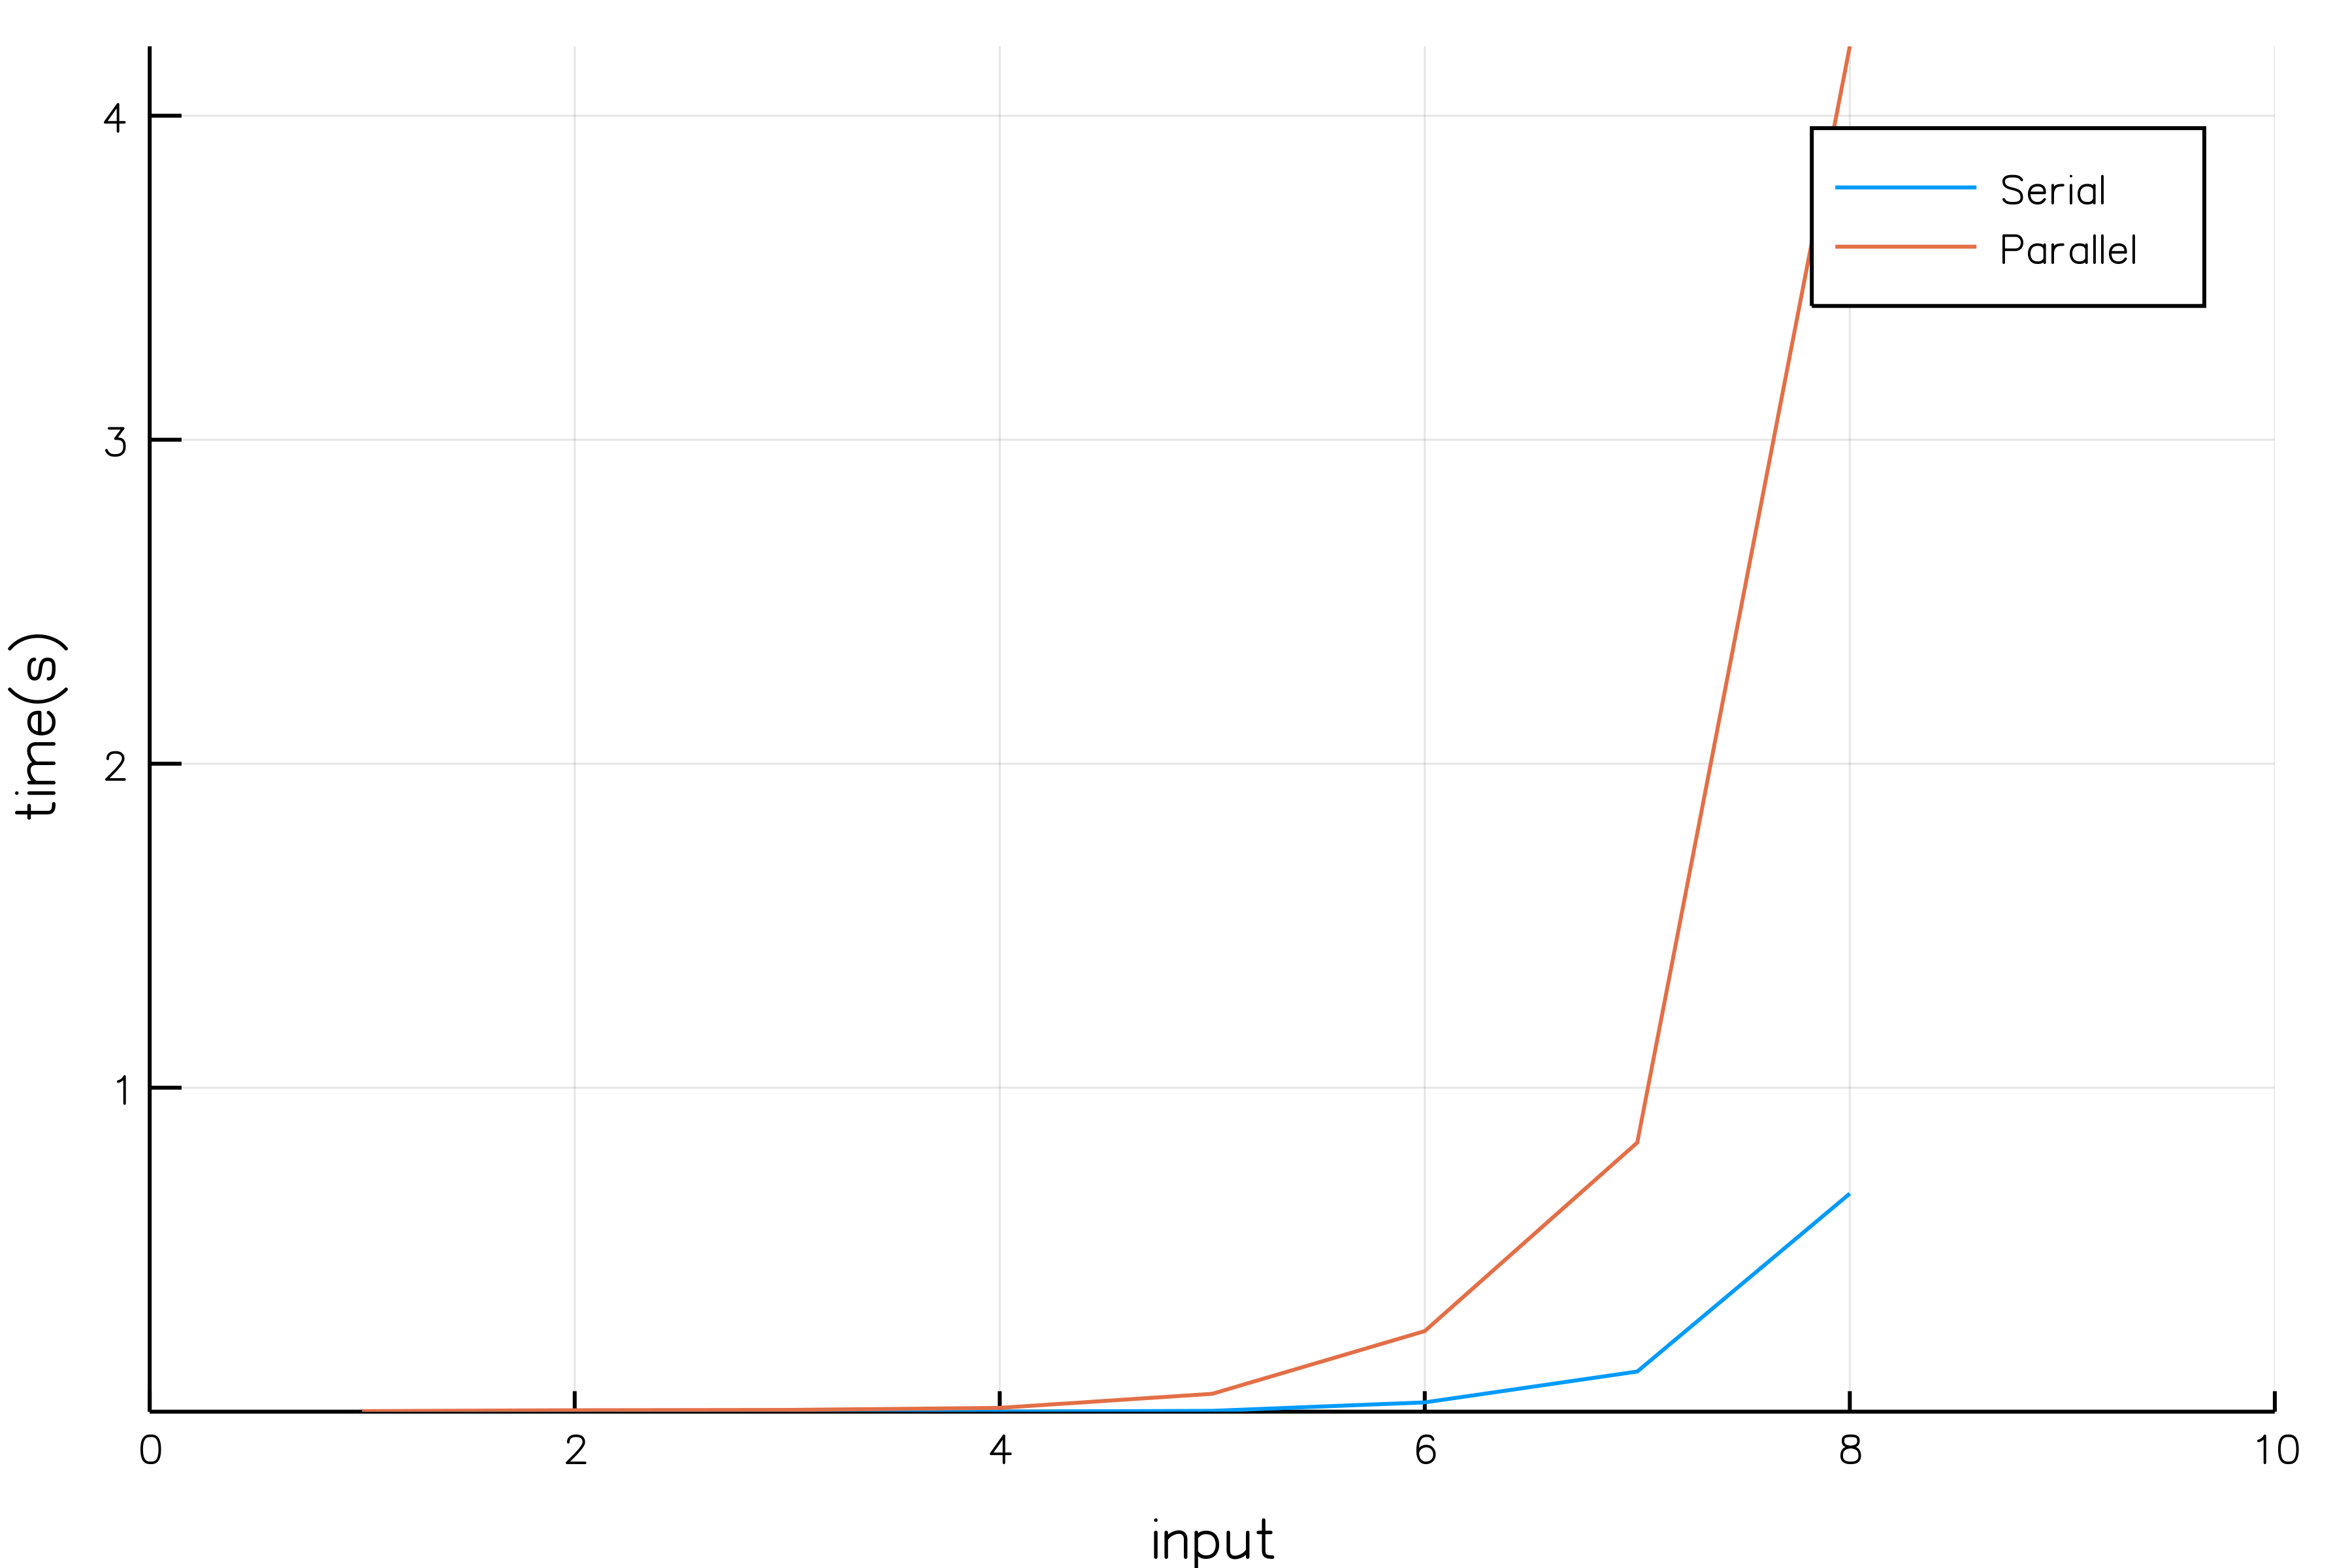
\includegraphics[scale=0.08]{traversalC.png}
\caption{Compared execution time of function traversal}
\end{figure}

\noindent\textbf{Execution time on Tesla}
\begin{Verbatim}[fontsize=\footnotesize]
input=[1,10,20,50,10^2,2*10^2,5*10^2,10^3,2*10^3]

function timeTraversal(model,input)
   t=Array{Float64}(length(input))
   pt=Array{Float64}(length(input))
   for i in range(1,length(input))
      structo=addn2D(input[i],model)
      pstructo=pStruct(structo.body)
      dim=checkStruct(structo.body)
      traversal(eye(dim+1),[],structo,[])
      ptraversal(eye(dim+1),[],pstructo,[])
      pt[i]=@elapsed ptraversal(eye(dim+1),[],pstructo,[])
      t[i]=@elapsed traversal(eye(dim+1),[],structo,[])
   end
   return t,pt
end

y,yp=timeTraversal(square,input)


p=plot(y,xaxis="input",yaxis="time",xlims=(0,length(input)+1),ylims=(0,maximum(y)+0.5),
  label=["Serial"],lw=2)  
pp=plot(yp,xaxis="input",yaxis="time",xlims=(0,length(input)+1),
       ylims=(0,maximum(y)+0.5),label=["Parallel"],lw=2)
\end{Verbatim}
\begin{figure*}[!h]
\centering
\subfloat[Serial]{%
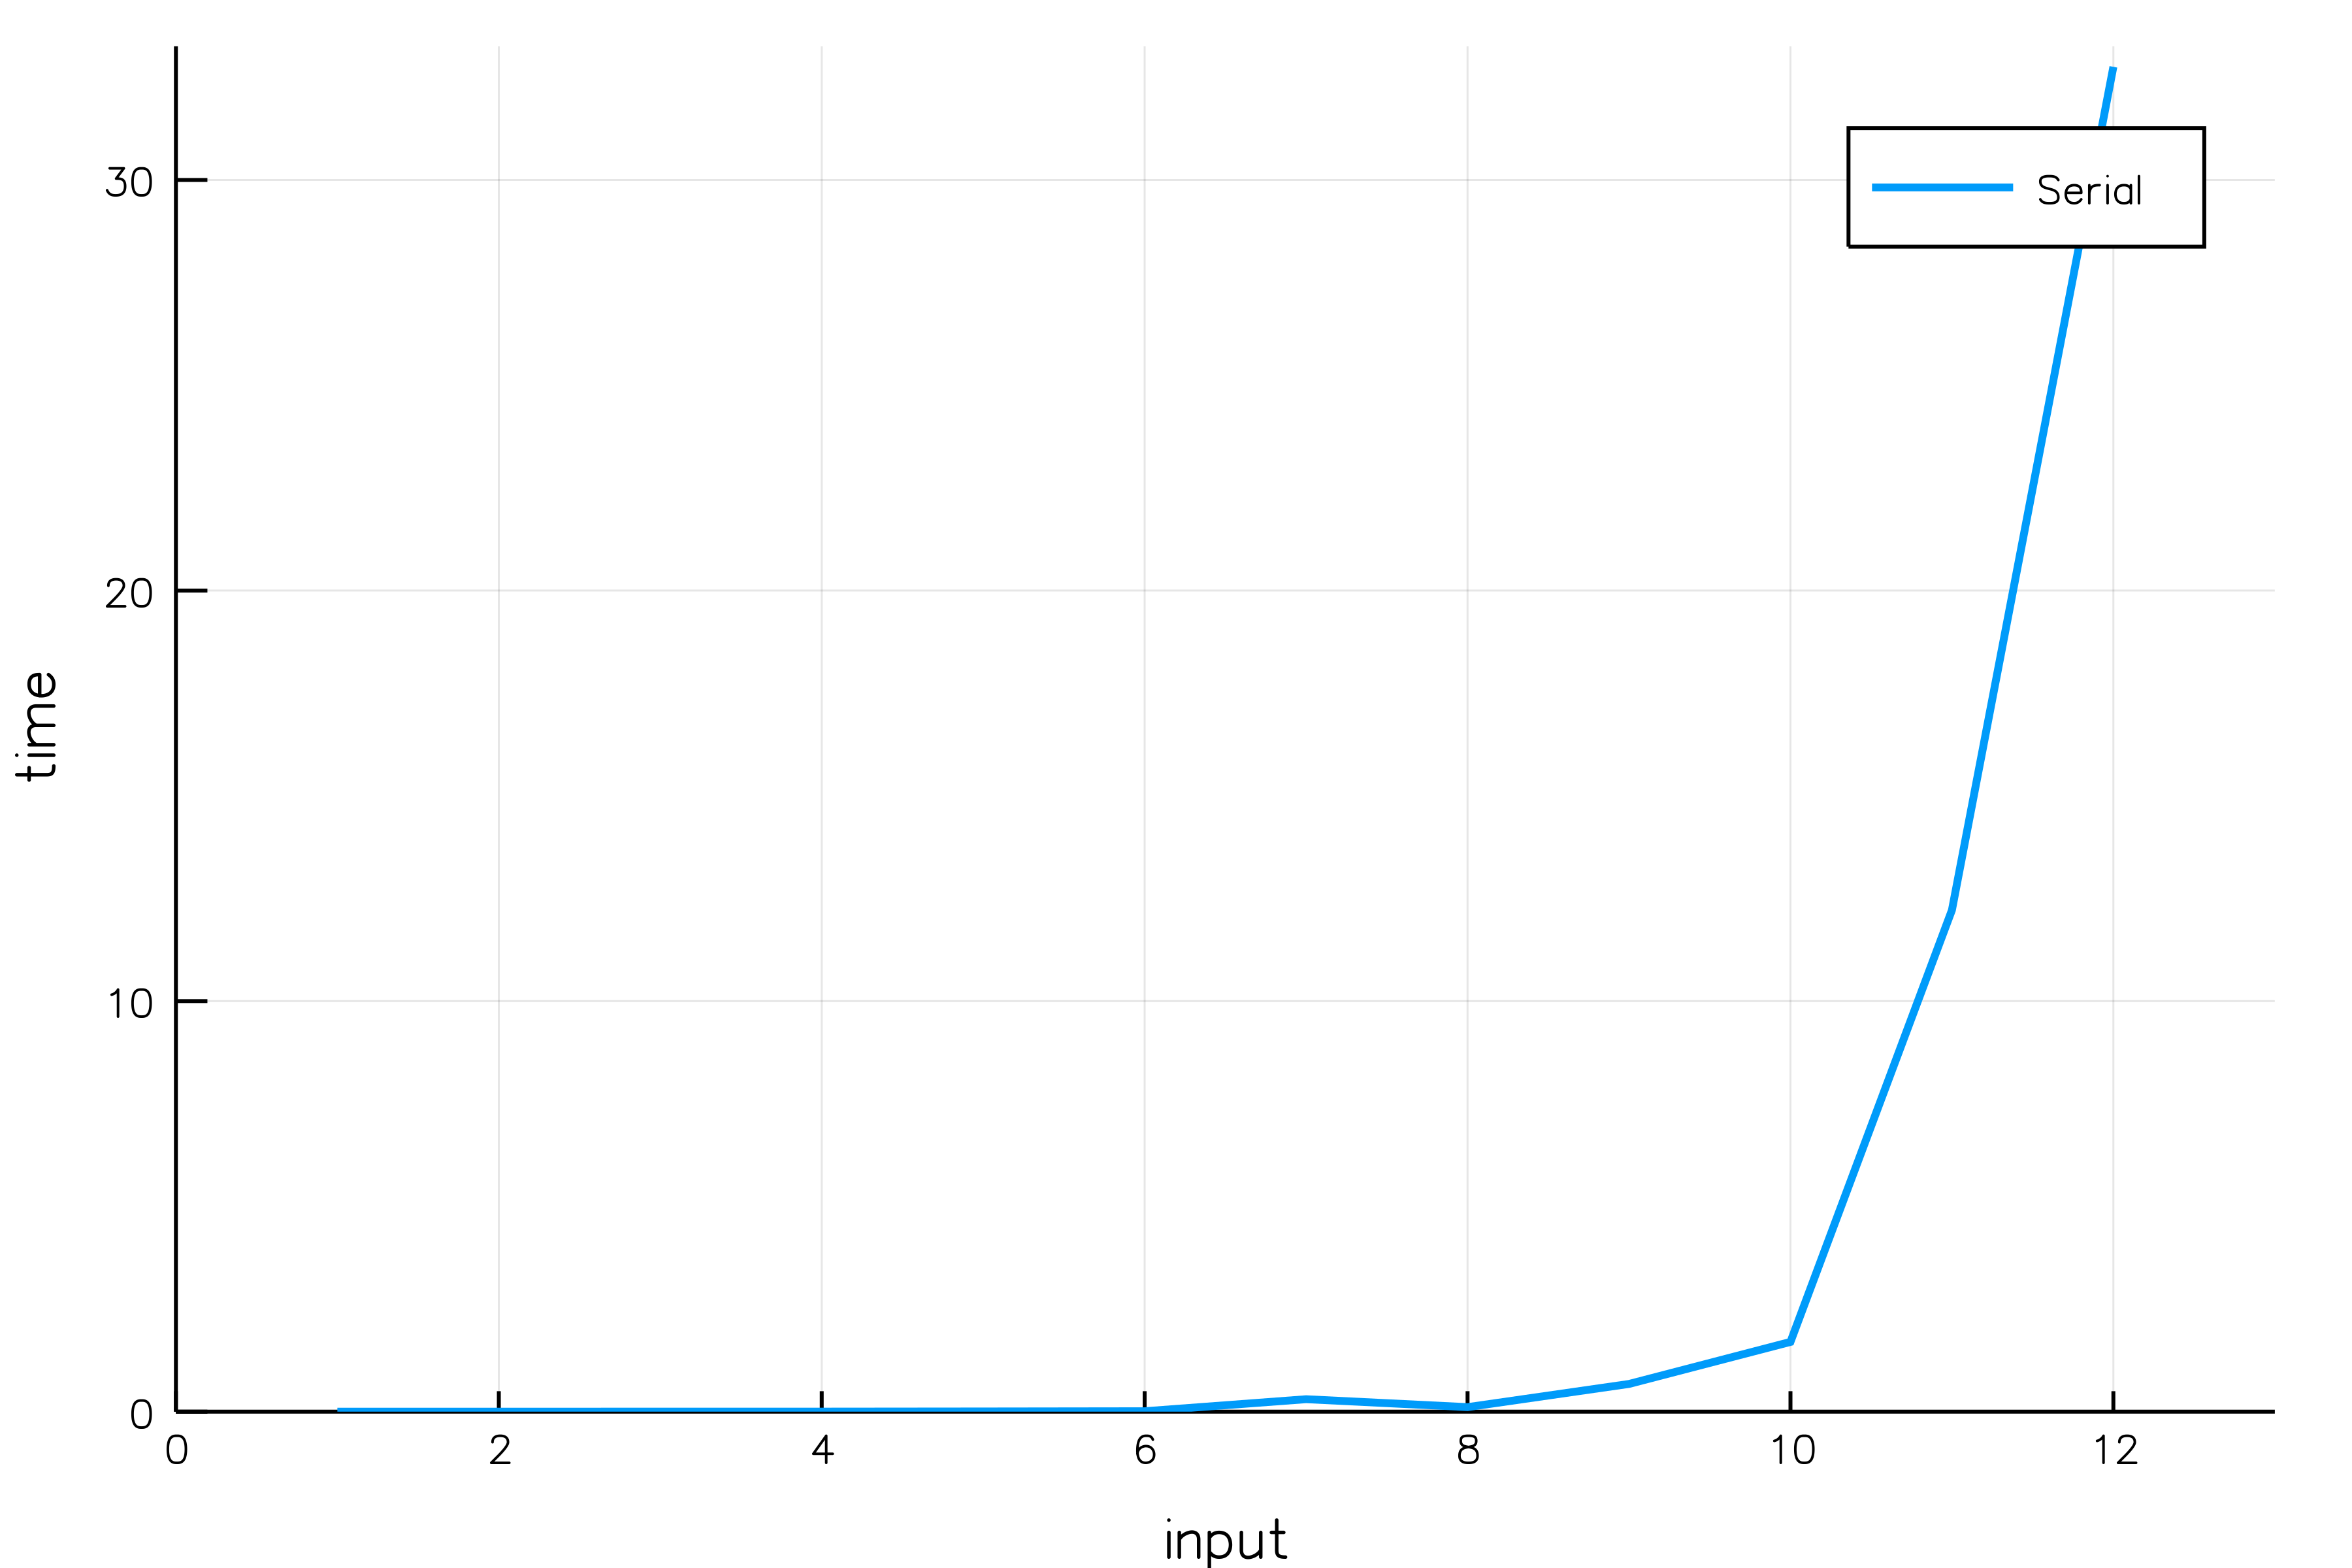
\includegraphics[scale=0.060]{traversal.png}
}
\subfloat[Parallel]{%
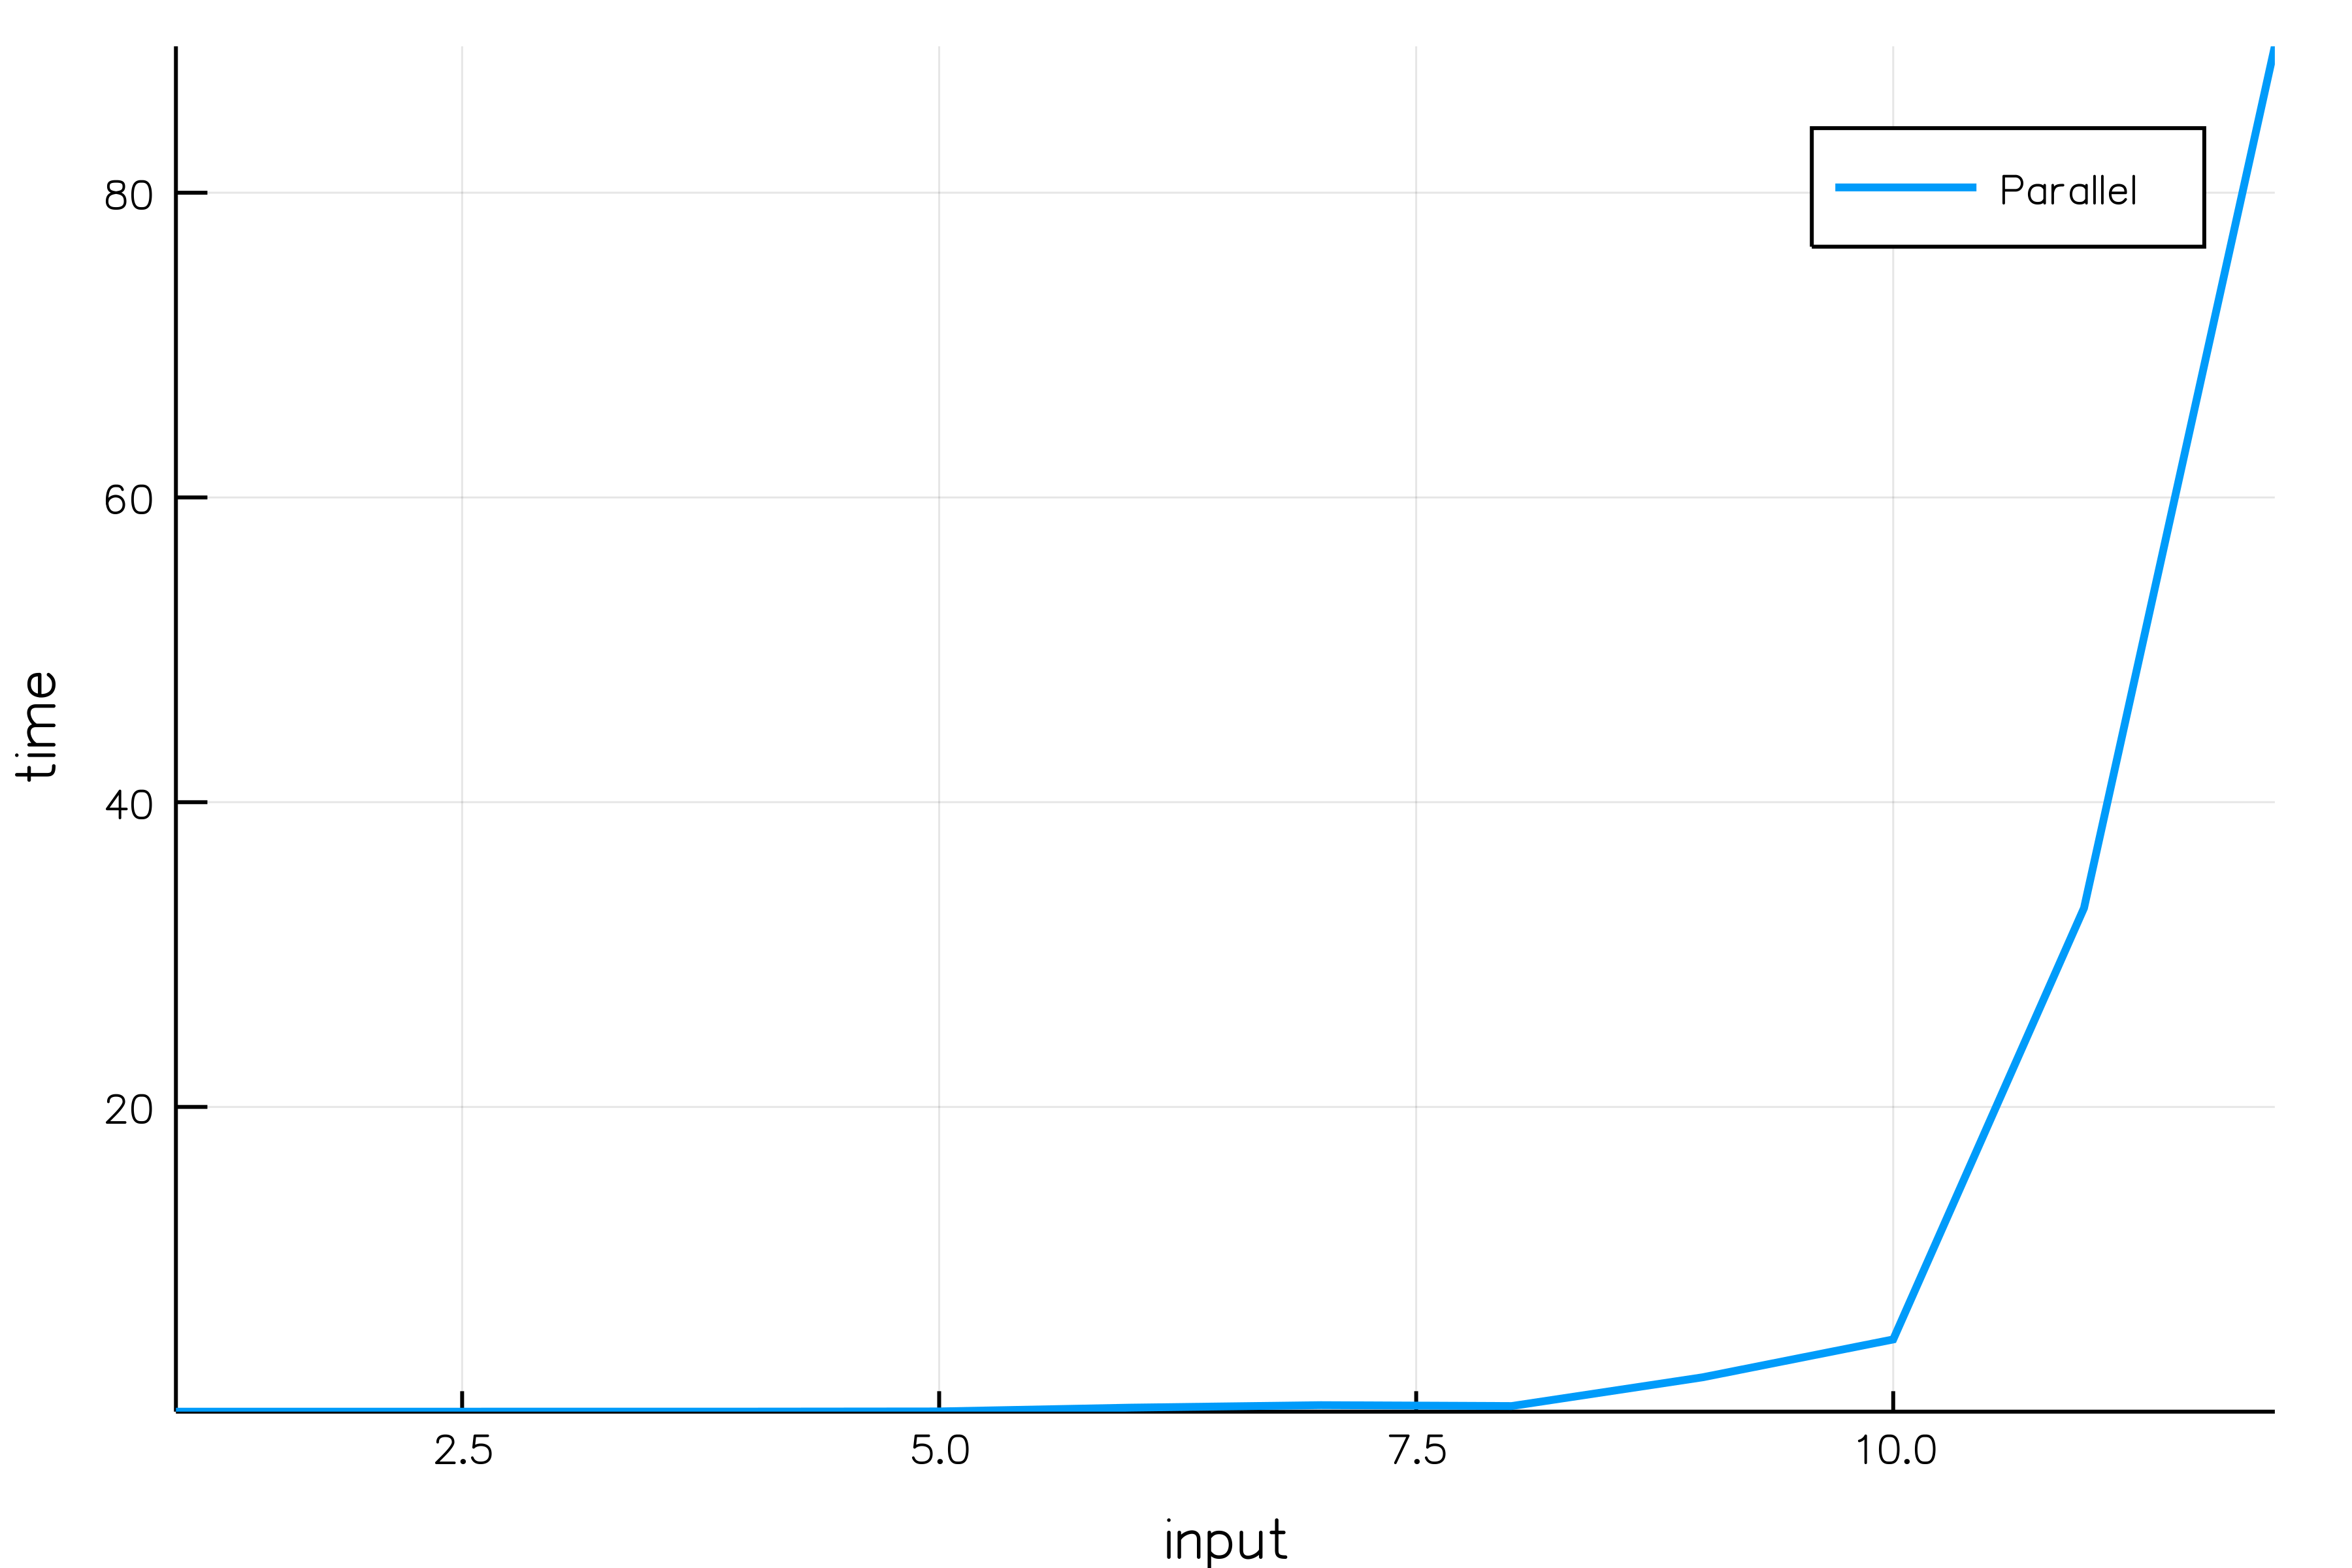
\includegraphics[scale=0.060]{ptraversal.png}
}
\caption{Execution time of function traversal on Tesla}
\end{figure*}

\noindent \framebox[42em][c]{Compare}
\begin{Verbatim}[fontsize=\footnotesize]
yc=[y,yp]
pc=plot(yc,label=["Serial" "Parallel"])
\end{Verbatim}

\begin{figure}[!h]
\centering
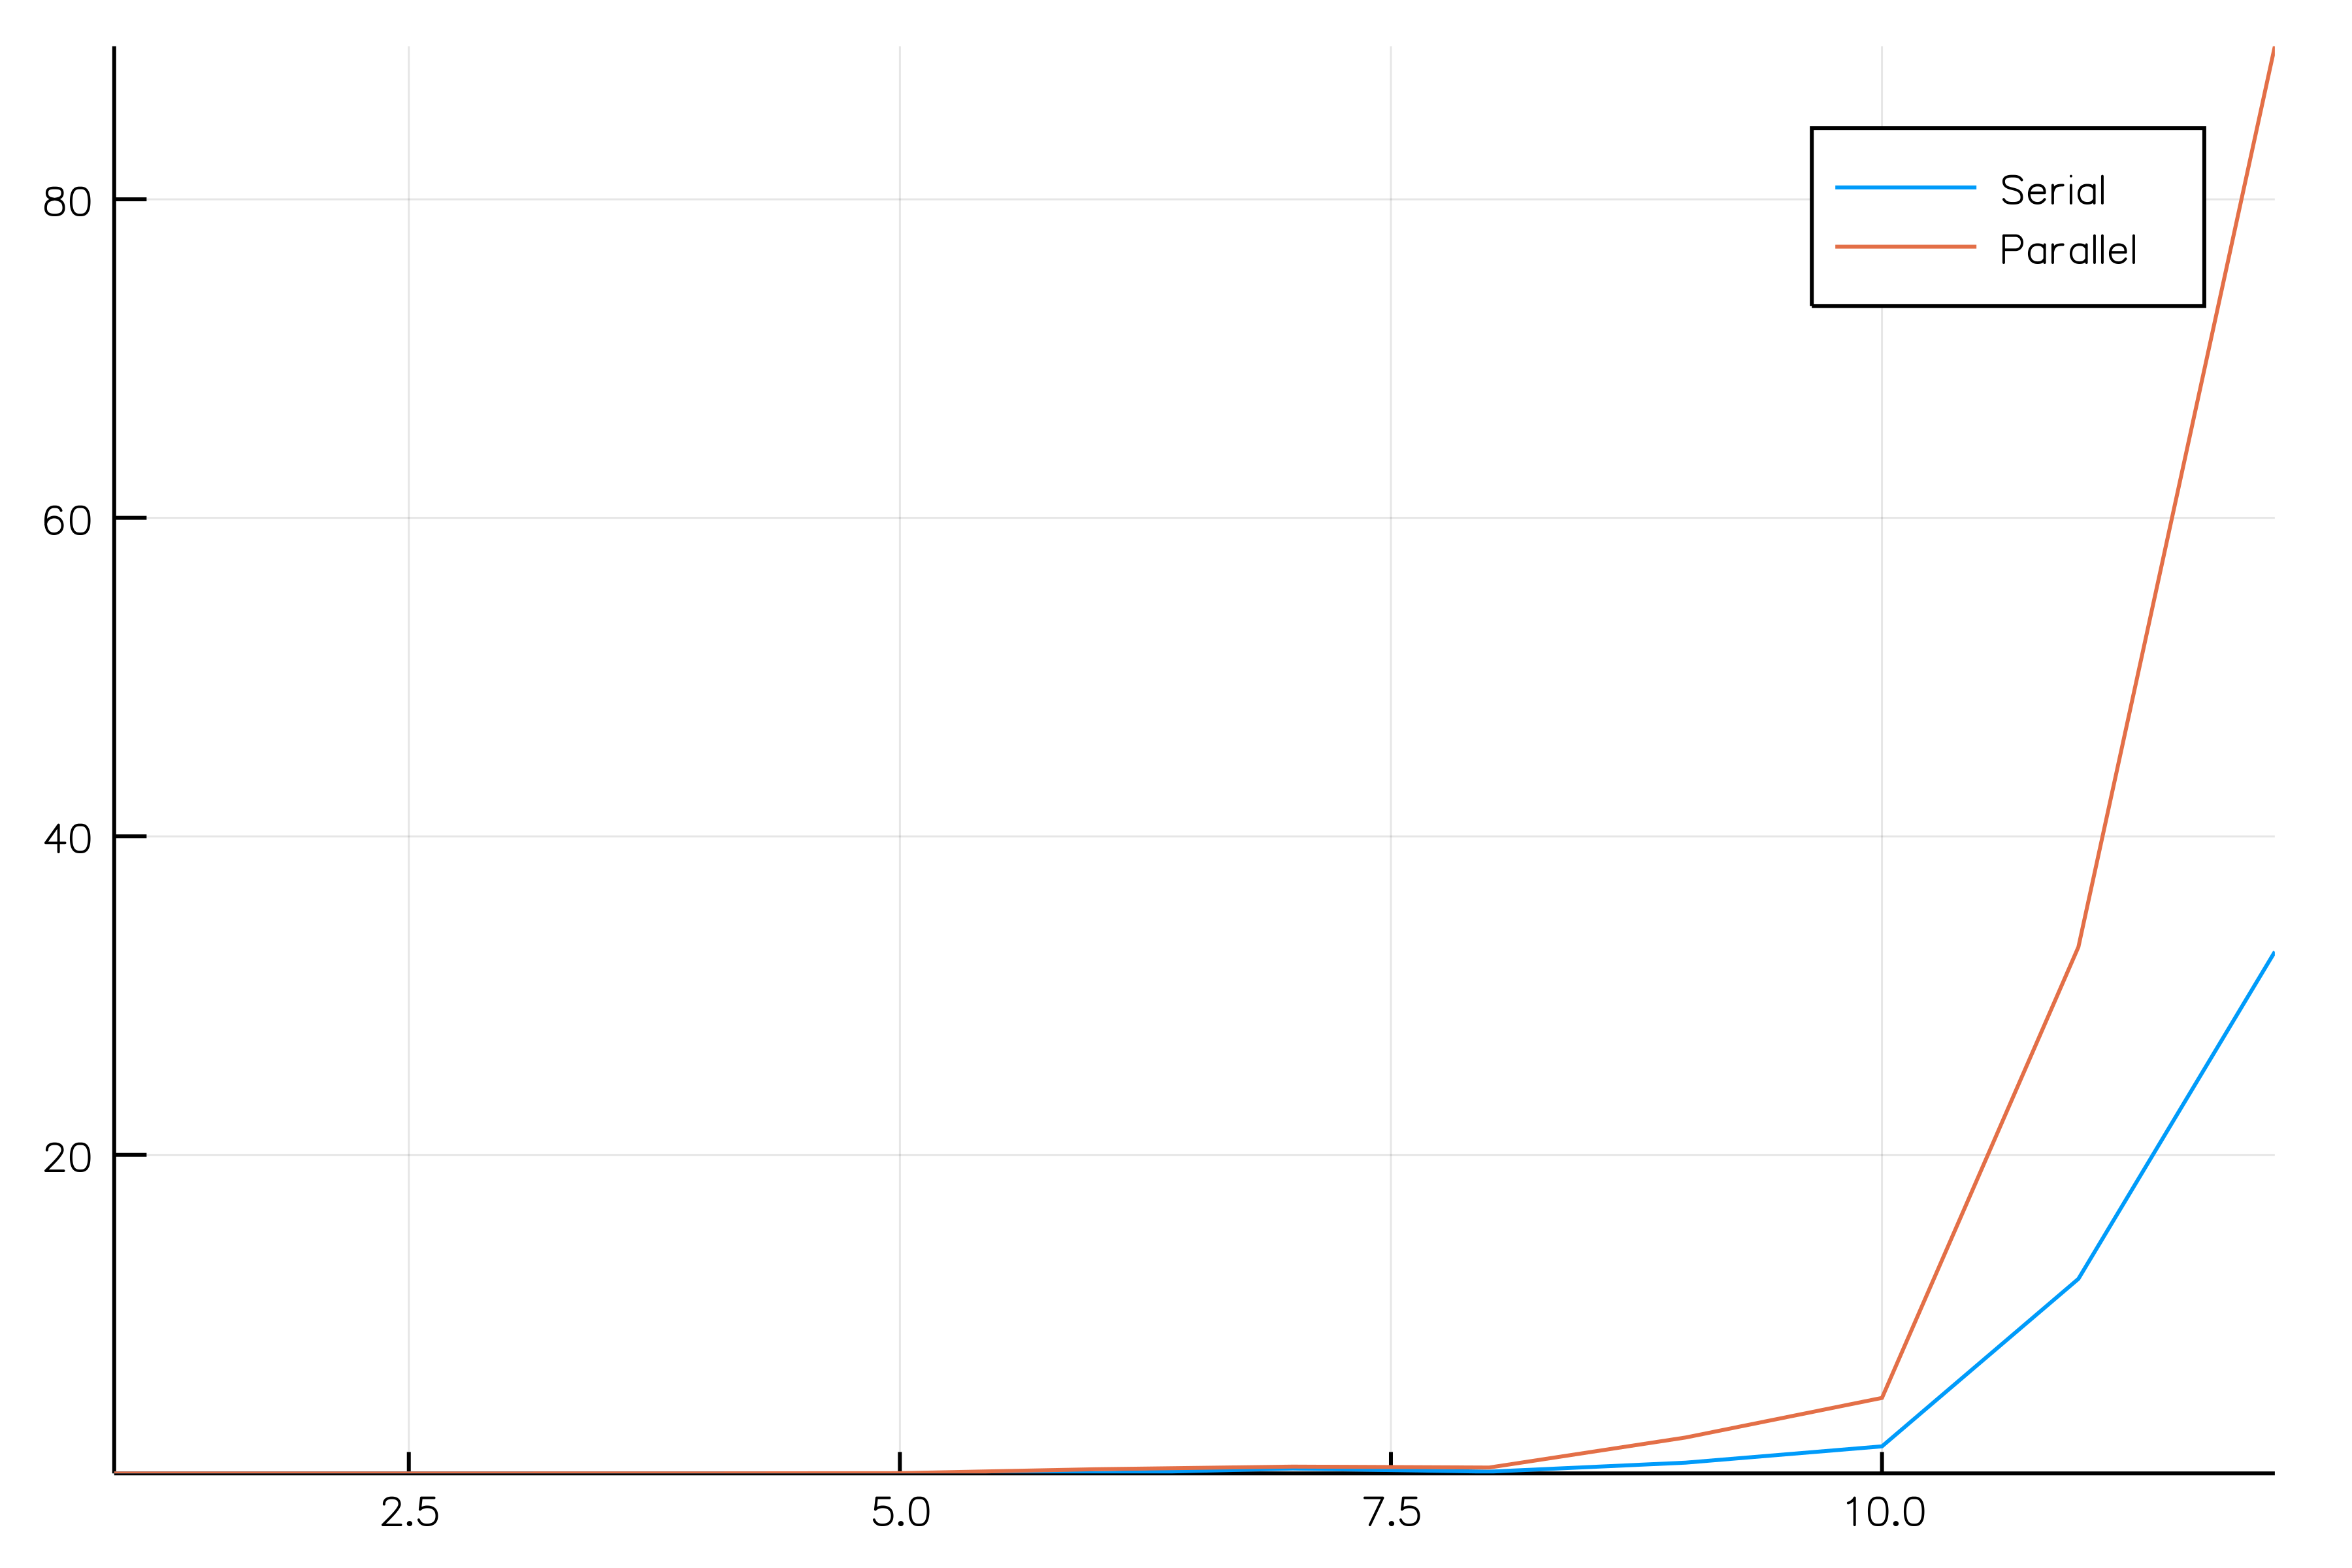
\includegraphics[scale=0.08]{comptraversal.png}
\caption{Compared execution time of function traversal on Tesla}
\end{figure}

%___________________________________________________________________________________________________________________________________

\newpage
\subsection{Struct}\label{Struct}
\subsubsection{Conversion}

\noindent \framebox[42em][c]{evalStruct}

\begin{multicols}{2}
\noindent \framebox[5em][c]{\textbf{\normalsize Python}}
\begin{Verbatim}[fontsize=\scriptsize]
def evalStruct(struct):
  dim = checkStruct(struct.body)
  CTM, stack = scipy.identity(dim+1), []
  scene = traversal(CTM, stack, struct, [])
  return scene    
\end{Verbatim}
\columnbreak
\framebox[5em][c]{\textbf{\normalsize Julia}}
\begin{Verbatim}[fontsize=\scriptsize]
function evalStruct(self)
  dim = checkStruct(self.body)
  CTM, stack = eye(dim+1), []
  scene = traversal(CTM, stack, self, []) 
  return scene
end
\end{Verbatim}
\end{multicols}

\noindent \framebox[5em][c]{\textbf{\normalsize Python}}
\begin{Verbatim}[fontsize=\footnotesize]

class Struct:
  def __init__(self,data=None,name=None,category=None):
    if data==None or data==[ ]:
      self.body = [ ]
    else:
      #self.body = [item for item in data if item != None]
      self.body = [item for item in data]
      self.box = box(self)
      self.dim = len(self.box[0])
    if name != None:
      self.name = str(name)
    else:
      self.name = str(id(self))
    if category != None:
      self.category = str(category)
    else:
      self.category = "feature"
  def __name__(self):
    return self.name
  def __category__(self):
    return self.category
  def __iter__(self):
    return iter(self.body)
  def __len__(self):
    return len(list(self.body))
  def __getitem__(self,i):
    return list(self.body)[i]}
  def __setitem__(self,i,value):
    self.body[i] = value
  def __print__(self): 
    return "<Struct name: %s>" % self.__name__()
  def __repr__(self):
    return "<Struct name: %s>" % self.__name__()
  def set_name(self,name):
    self.name = str(name)
  def clone(self,i=0):
    from copy import deepcopy
    newObj = deepcopy(self)
    if i != 0: newObj.name = self.name + "_" + str(i)
    return newObj
  def set_category(self,category):
    self.category = str(category)
\end{Verbatim}

\framebox[5em][c]{\textbf{\normalsize Julia}}
\begin{Verbatim}[fontsize=\footnotesize]

type Struct
  body::Array
  box
  name::AbstractString
  dim
  category::AbstractString
  function Struct()
    self=new([],Nullable{Any},"new",Nullable{Any},"feature")
    self.name=string(object_id(self))
    return self
  end
  function Struct(data::Array)
    self=Struct()
    self.body=data
    self.box=box(self)
    self.dim=length(self.box[1])
    return self
  end
  function Struct(data::Array,name)
    self=Struct()
    self.body=[item for item in data]
    self.box=box(self)
    self.dim=length(self.box[1])
    self.name=string(name)
    return self
  end
  function Struct(data::Array,name,category)
    self=Struct()
    self.body=[item for item in data]
    self.box=box(self)
    self.dim=length(self.box[1])
    self.name=string(name)
    self.category=string(category)
    return self
  end
end
function name(self::Struct)
  return self.name
end
function category(self::Struct)
  return self.category
end
function len(self::Struct)
  return length(self.body)
end
function getitem(self::Struct,i::Int)
  return self.body[i]
end
function setitem(self::Struct,i,value)
  self.body[i]=value
end
function pprint(self::Struct)
  return "<Struct name: $(self.__name__())"
end
function set_name(self::Struct,name)
  self.name=string(name)
end
function clone(self::Struct,i=0)
    newObj=deepcopy(self)
    if i!=0
      newObj.name="$(self.__name__())_$(string(i))"
    end
    return newObj
end
function set_category(self::Struct,category)
  self.category=string(category)
end
\end{Verbatim}

\subsubsection{Parallelization}
\begin{Verbatim}[fontsize=\footnotesize]

function pevalStruct(self)
  dim = pcheckStruct(self.body)
  CTM, stack = eye(dim+1), []
  scene = ptraversal(CTM, stack, self, []) 
return scene
end

\end{Verbatim}
\begin{Verbatim}[fontsize=\footnotesize]

@everywhere type pStruct
  body::Array
  box
  name::AbstractString
  dim
  category::AbstractString
  function pStruct()
    self=new([],Nullable{Any},"new",Nullable{Any},"feature")
    self.name=string(object_id(self))
    return self
  end
  function pStruct(data::Array)
    self=pStruct()
    self.body=data
    self.box=pbox(self)
    self.dim=length(self.box[1])
    return self
  end
  function pStruct(data::Array,name)
    self=pStruct()
    self.body=[item for item in data]
    self.box=pbox(self)
    self.dim=length(self.box[1])
    self.name=string(name)
    return self
  end
  function pStruct(data::Array,name,category)
    self=pStruct()
    self.body=[item for item in data]
    self.box=pbox(self)
    self.dim=length(self.box[1])
    self.name=string(name)
    self.category=string(category)
    return self
  end
end
function name(self::pStruct)
  return self.name
end
function category(self::pStruct)
  return self.category
end
function len(self::pStruct)
  return length(self.body)
end
function getitem(self::pStruct,i::Int)
  return self.body[i]
end
function setitem(self::pStruct,i,value)
  self.body[i]=value
end
function pprint(self::pStruct)
  return "<Struct name: $(self.__name__())"
end
function set_name(self::pStruct,name)
  self.name=string(name)
end
function clone(self::pStruct,i=0)
  newObj=deepcopy(self)
  if i!=0
    newObj.name="$(self.__name__())_$(string(i))"
  end
  return newObj
end
function set_category(self::pStruct,category)
  self.category=string(category)
end
\end{Verbatim}

\subsubsection{Unit-Test}

\framebox[42em][c]{Serial Tests}
\begin{Verbatim}[fontsize=\footnotesize]

square=([[0,0],[0,1],[1,0],[1,1]],[[0,1,2,3]])

@testset "Struct Tests" begin
	@test Struct([square]).body==[square]
	@test Struct([square]).dim==length(square[1][1])
	@test Struct([square]).box==[[0,0],[1,1]]
end
\end{Verbatim}
\framebox[42em][c]{Parallel Tests}
\begin{Verbatim}[fontsize=\footnotesize]

square=([[0,0],[0,1],[1,0],[1,1]],[[0,1,2,3]])

@testset "pStruct Tests" begin
    @test pStruct([square]).body==[square]
    @test pStruct([square]).dim==length(square[1][1])
    @test pStruct([square]).box==[[0,0],[1,1]]
    @test pStruct([square]).category=="feature"
    @test pStruct([square],"quadrato").name=="quadrato"
end
\end{Verbatim}
\subsubsection{Results}
\textbf{Execution time on PC}
\begin{Verbatim}[fontsize=\footnotesize]
times=[]
ptimes=[]

append!(times,Time(Struct,[[l[i]]]) for i in range(1,length(l)) )
append!(ptimes,Time(pStruct,[[l[i]]]) for i in range(1,length(l)-1))

plot(times,xlabel="input",xlims=(0,length(times)+2),ylabel="time(s)",label=["Serial"])
plot(ptimes,xlabel="input",xlims=(0,length(times)+2),ylabel="time(s)",label=["Parallel"])

\end{Verbatim}
\begin{figure*}[!h]
\centering
\subfloat[Serial]{%
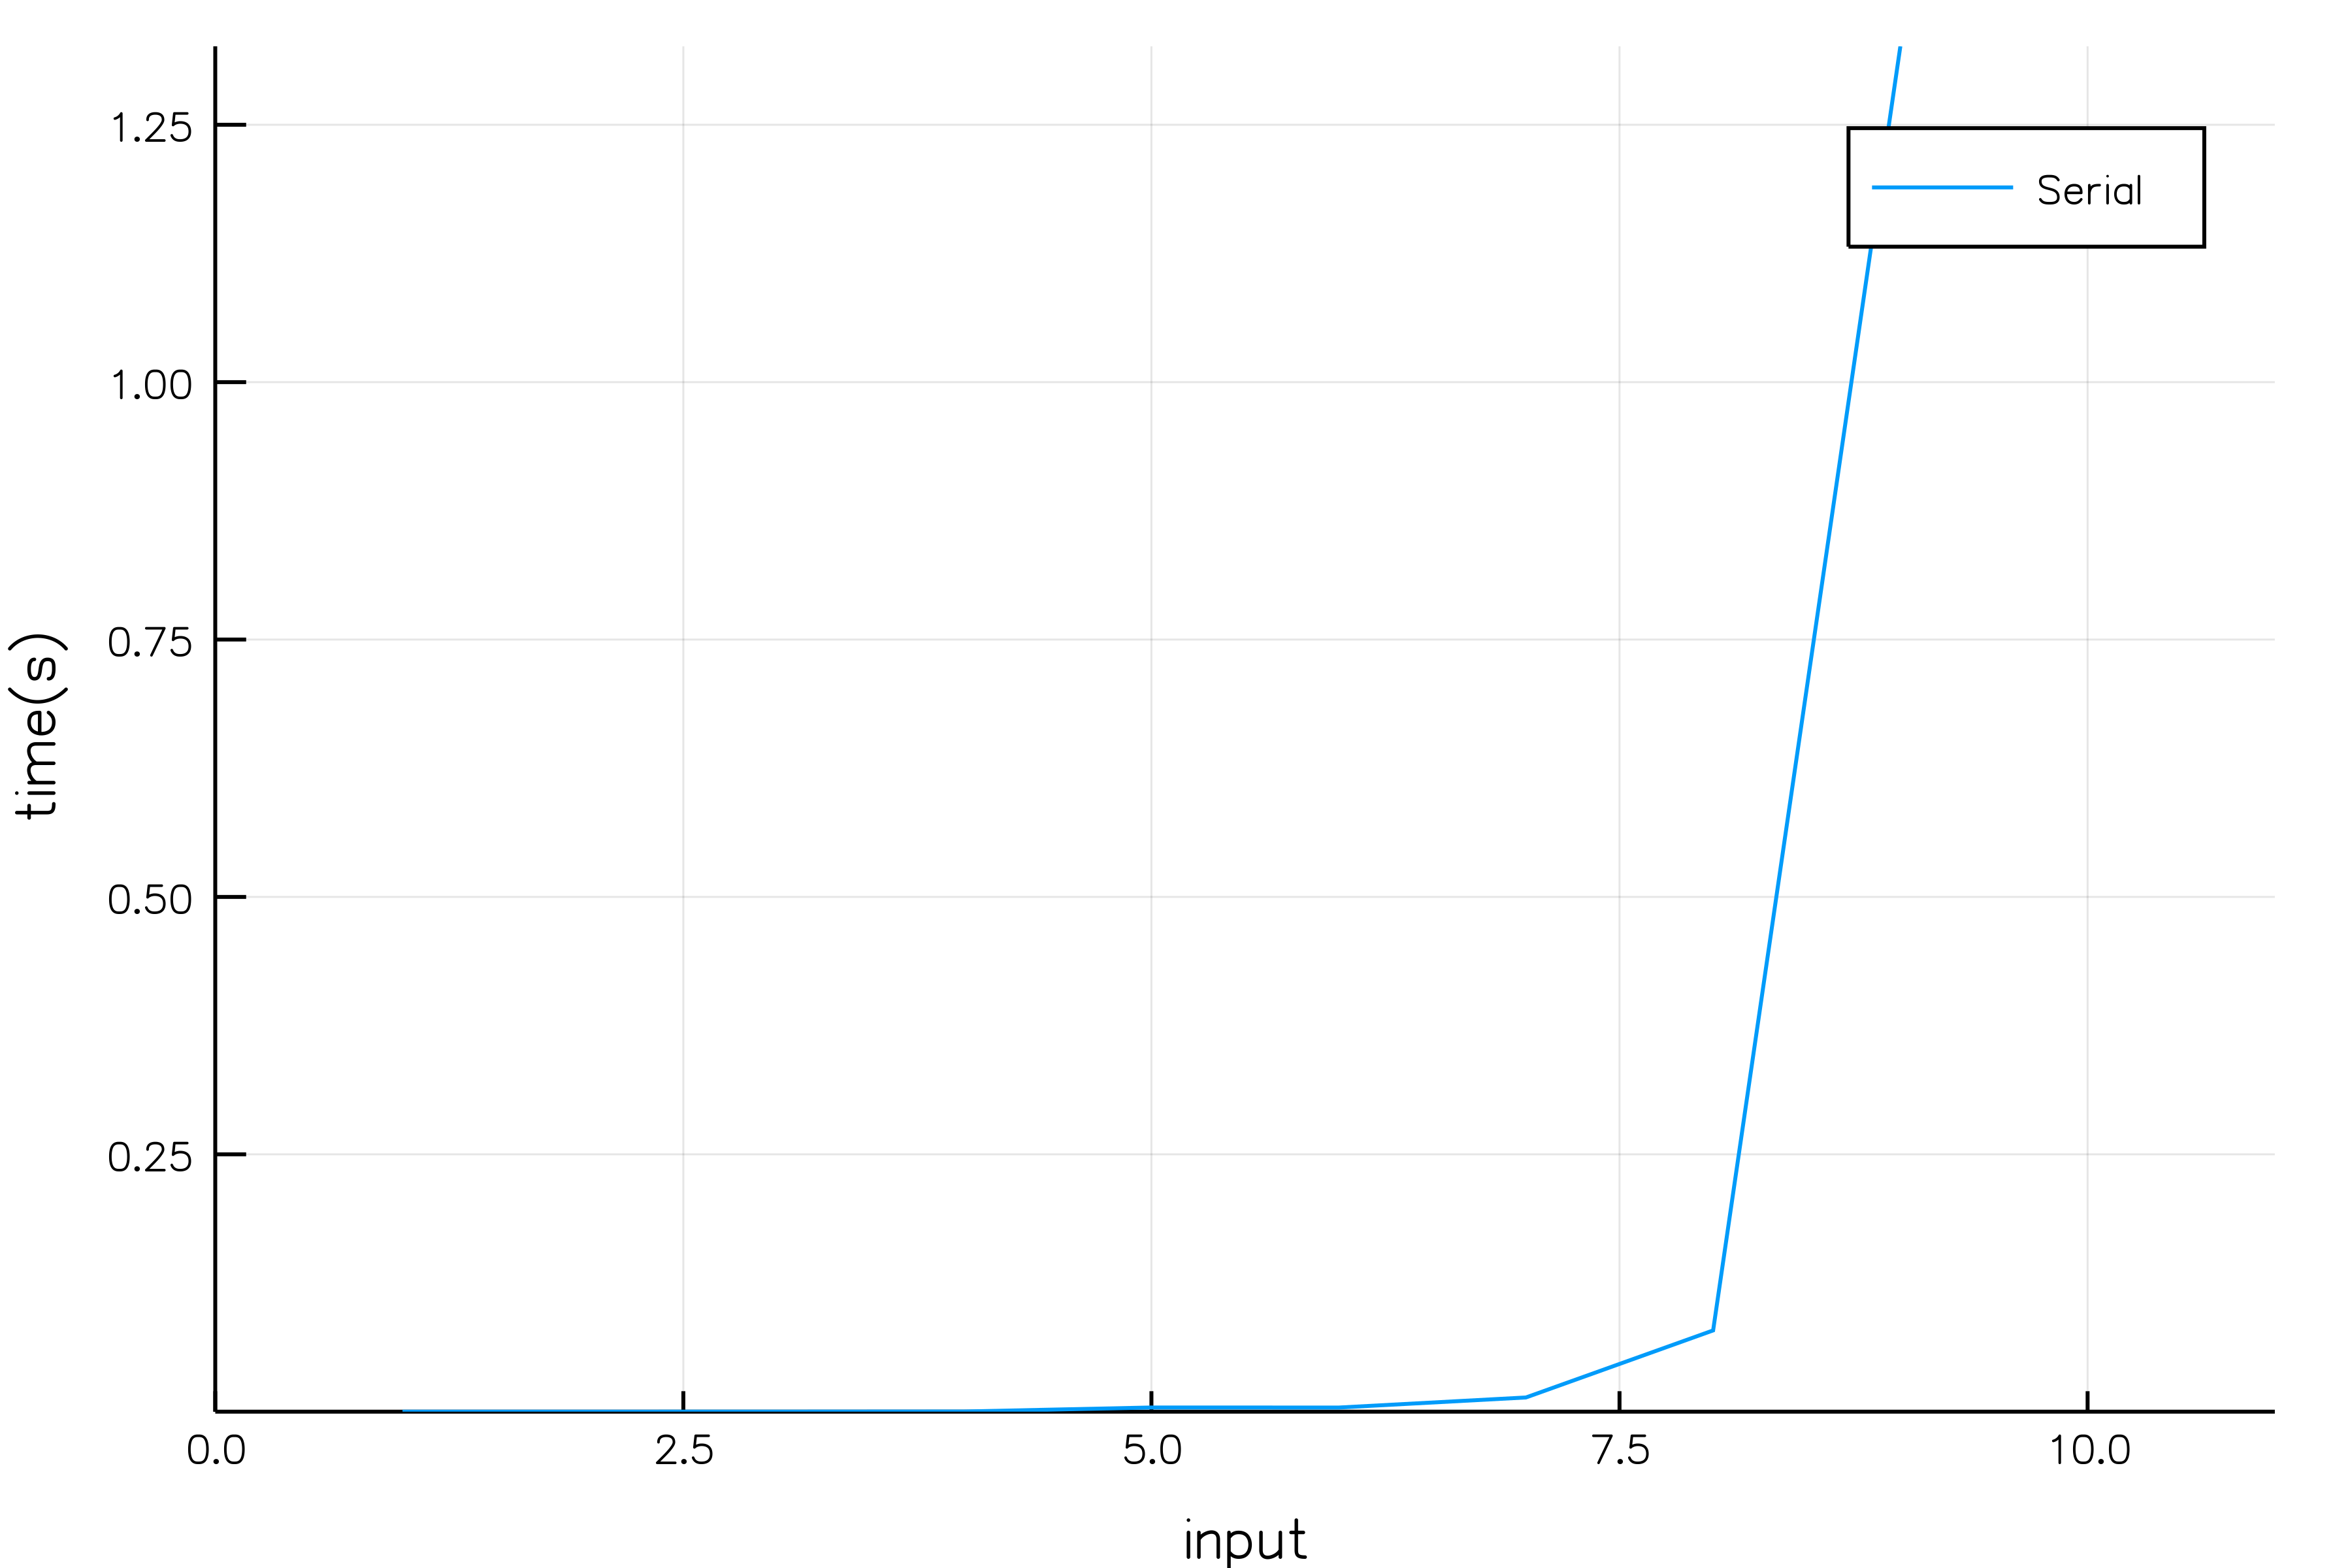
\includegraphics[scale=0.060]{Struct.png}
}
\subfloat[Parallel]{%
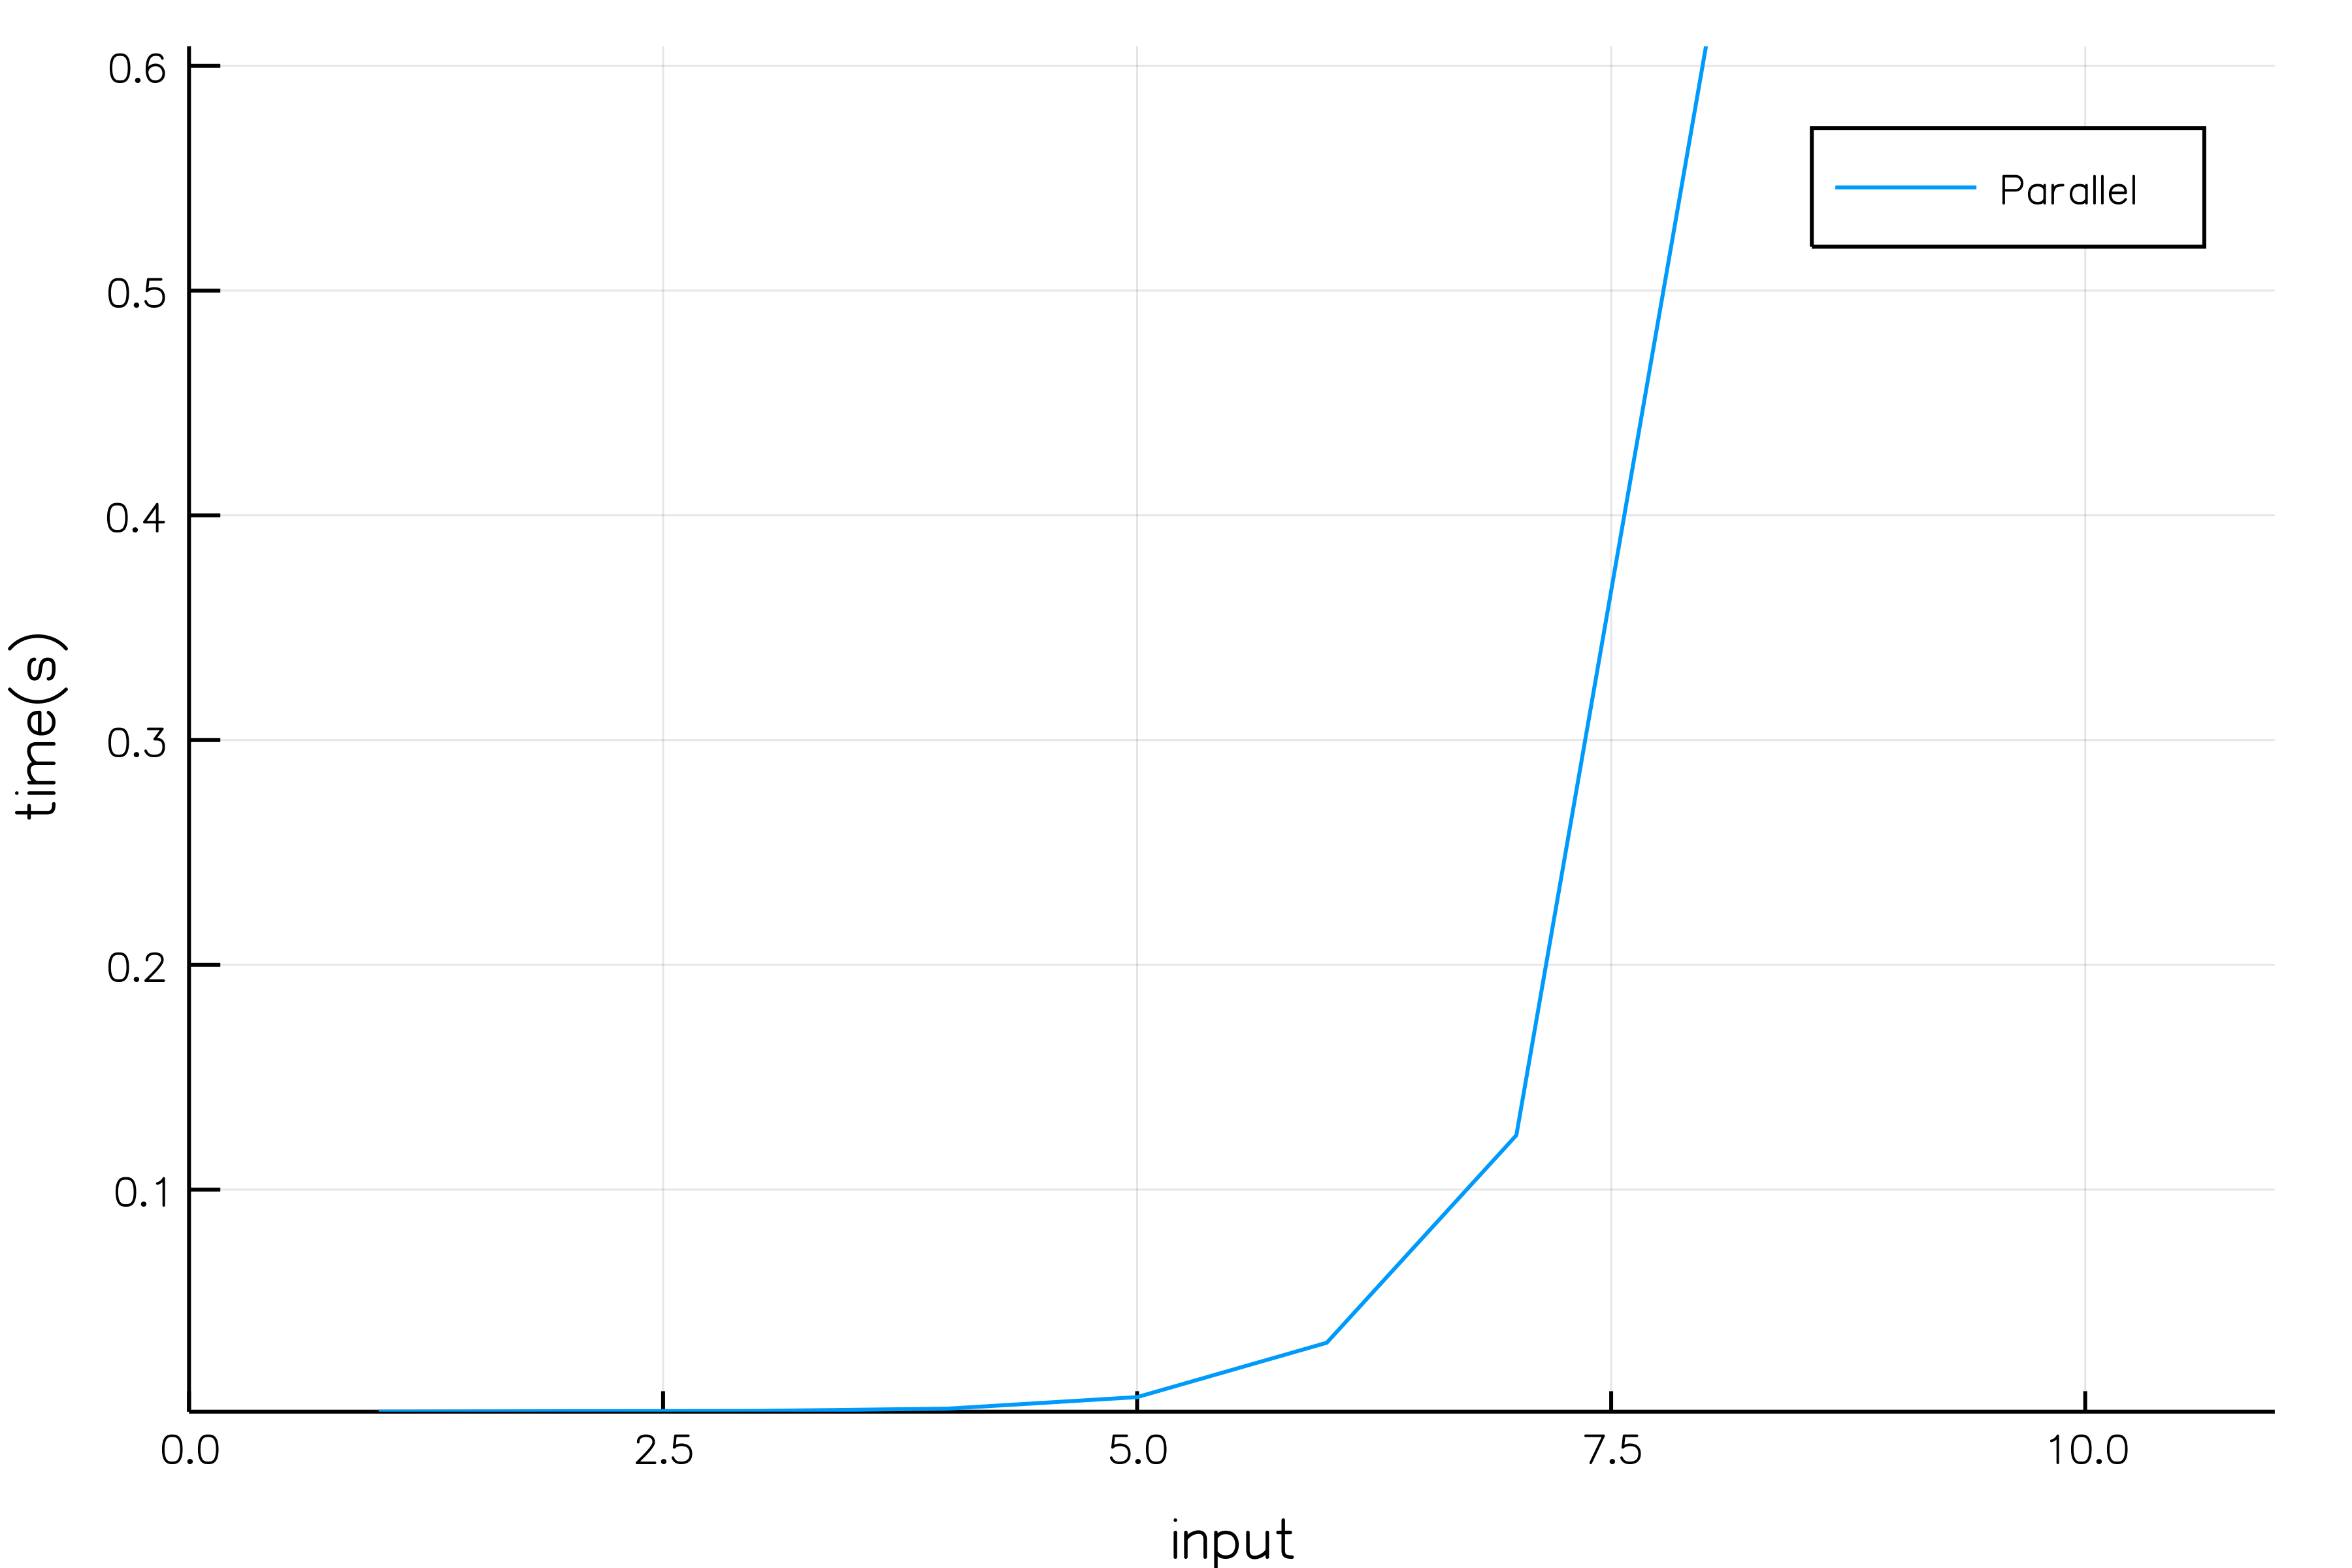
\includegraphics[scale=0.060]{StructParallel.png}
}
\caption{Execution time of function Struct}
\end{figure*}

\noindent\framebox[42em][c]{Compare}
\begin{Verbatim}[fontsize=\footnotesize]
plot([times,ptimes],xlabel="input",xlims=(0,length(times)+2),ylabel="time(s)",
label=["Serial","Parallel"])
\end{Verbatim}
\begin{figure}[!h]
\centering
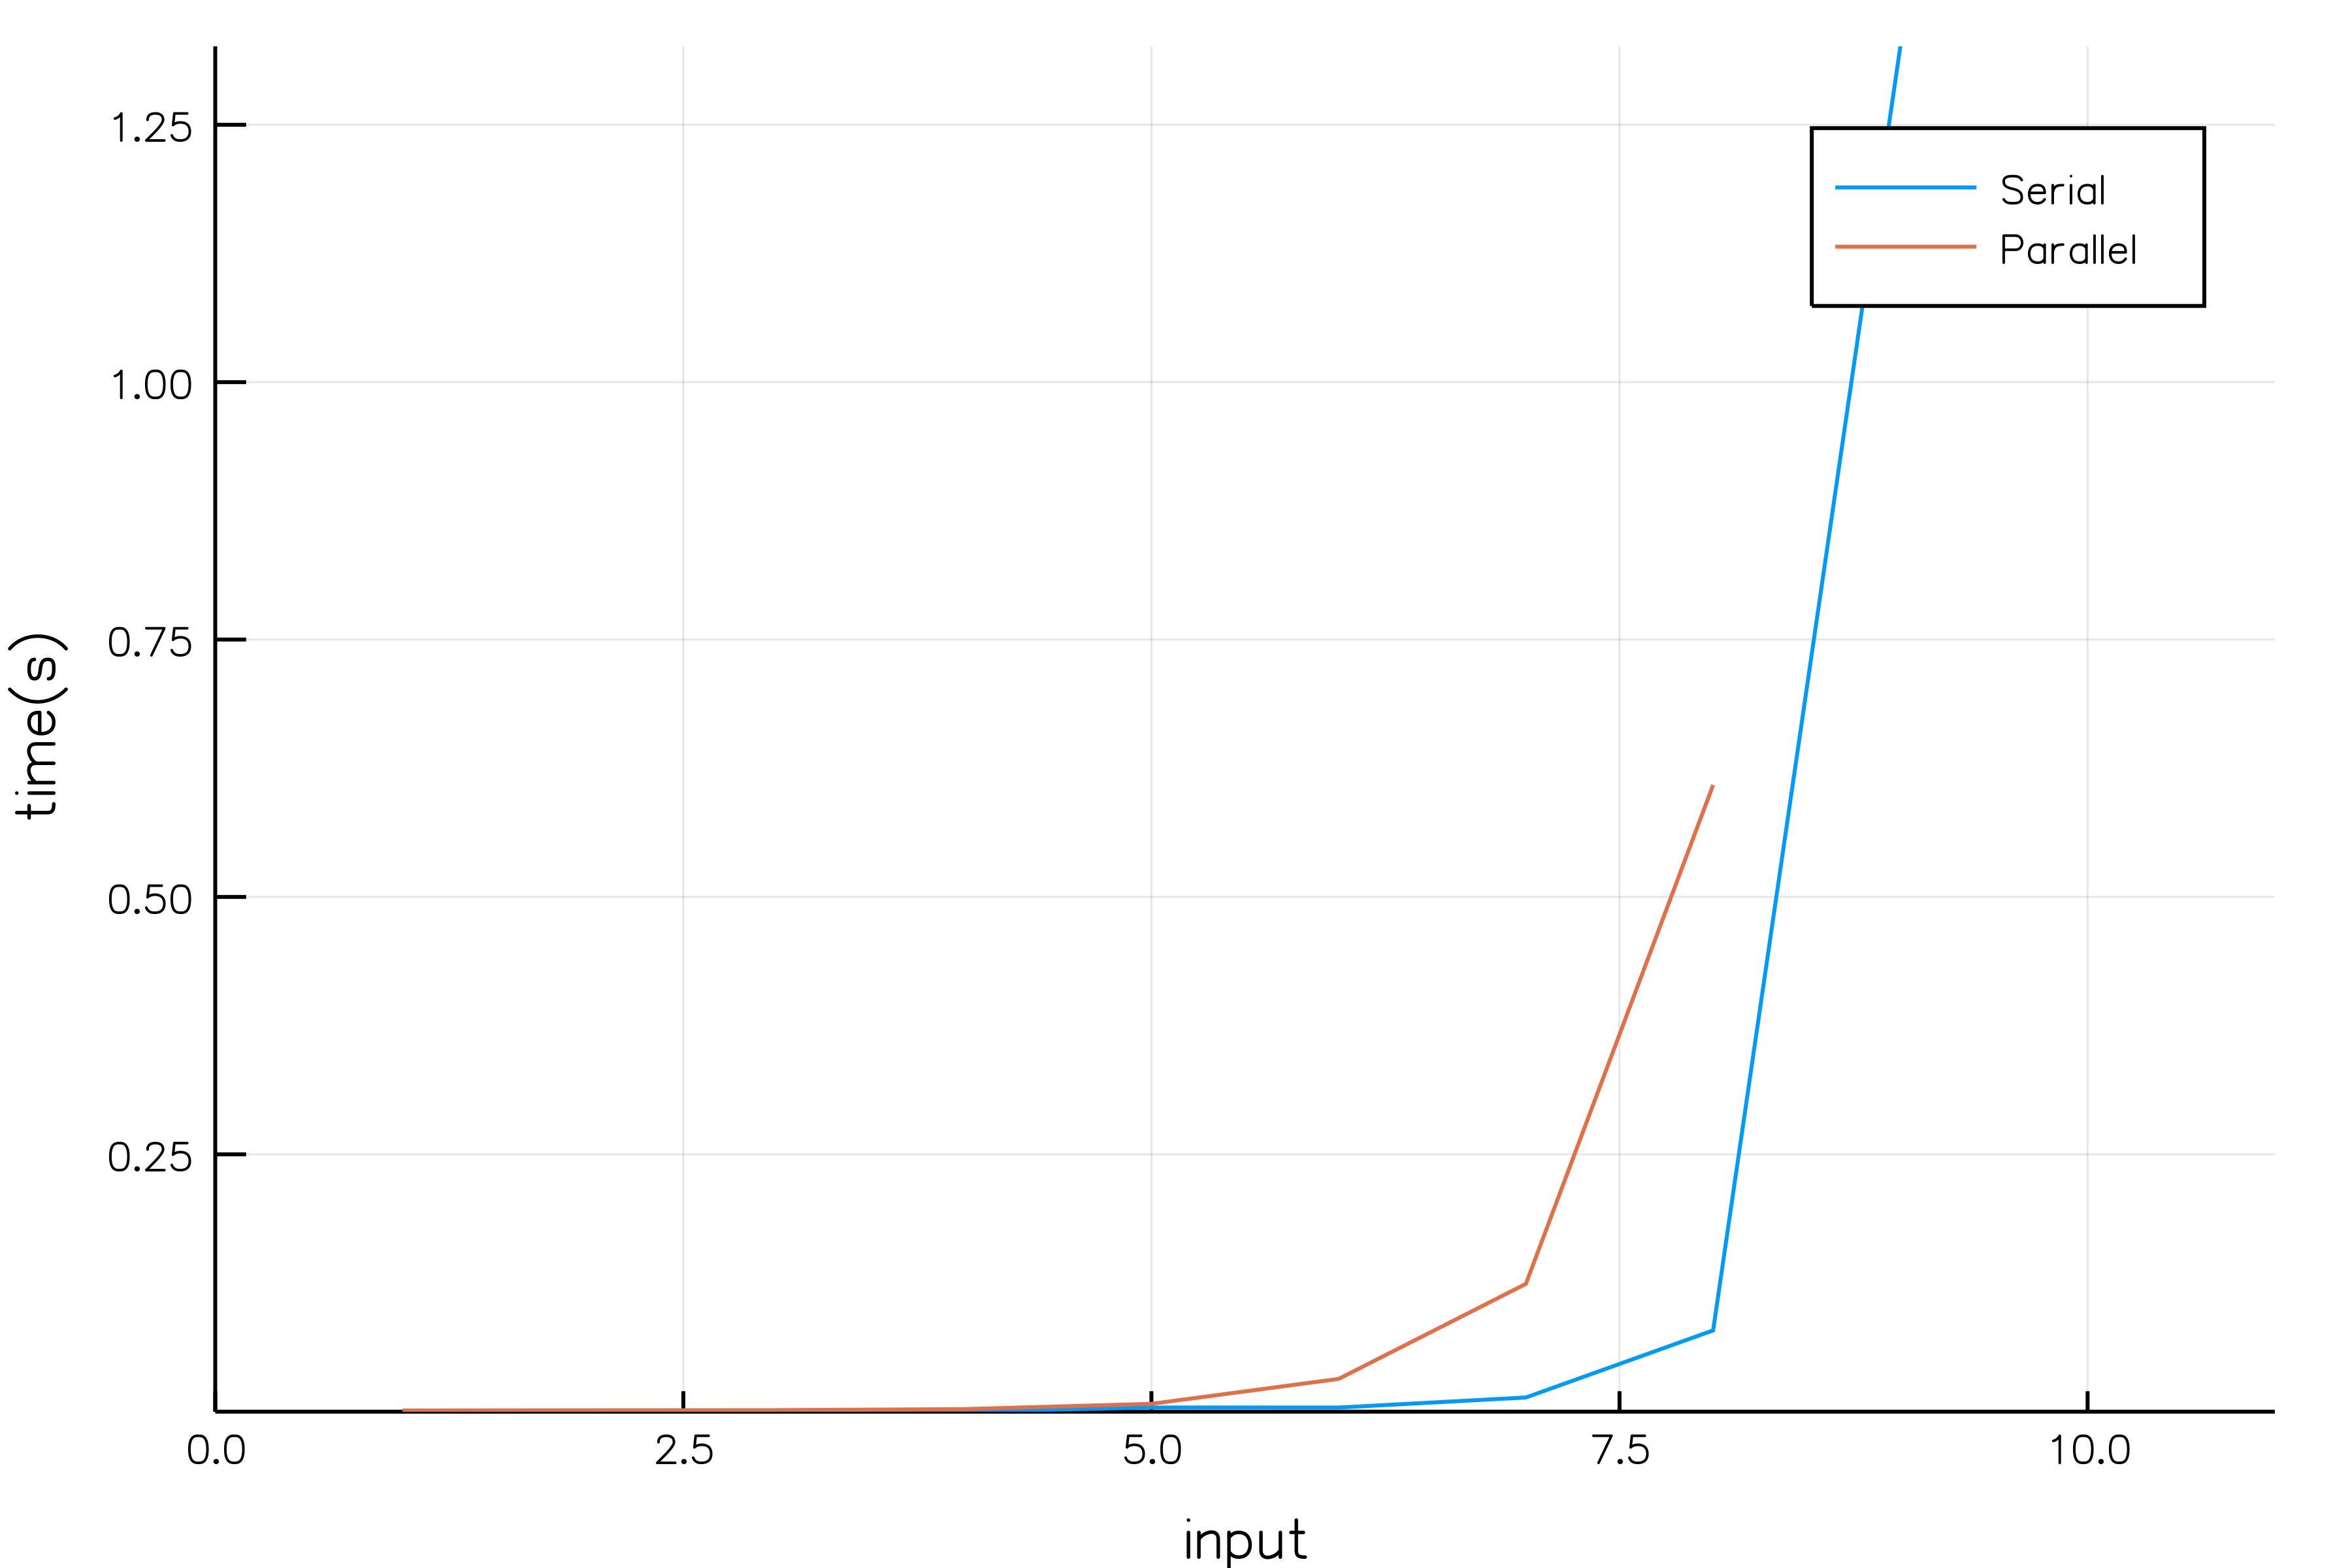
\includegraphics[scale=0.08]{StructC.png}
\caption{Compared execution time of function Struct}
\end{figure}
%__________________________________________________________________________________________________________________________
\newpage

\noindent\textbf{Execution time on Tesla}
\begin{Verbatim}[fontsize=\footnotesize]
input=[1,10,20,50,10^2,2*10^2,5*10^2,10^3,2*10^3]
function timeStruct(model,input)
  t=Array{Float64}(length(input))
  pt=Array{Float64}(length(input))
  for i in range(1,length(input))
    structo=addn2D(input[i],model)
    Struct(structo.body)
    pStruct(structo.body)
    t[i]=@elapsed  Struct(structo.body)
    pt[i]=@elapsed pStruct(structo.body)
  end
  return t,pt
end

y,yp=timeStruct(square,input)
p=plot(y,xaxis="input",yaxis="time",xlims=(0,length(input)+1),
       ylims=(0,maximum(y)+0.5), label=["Serial"],lw=2)
       
pp=plot(yp,xaxis="input",yaxis="time",xlims=(0,length(input)+1),
       ylims=(0,maximum(y)+0.5),label=["Parallel"],lw=2)
\end{Verbatim}
\begin{figure*}[!h]
\centering
\subfloat[Serial]{%
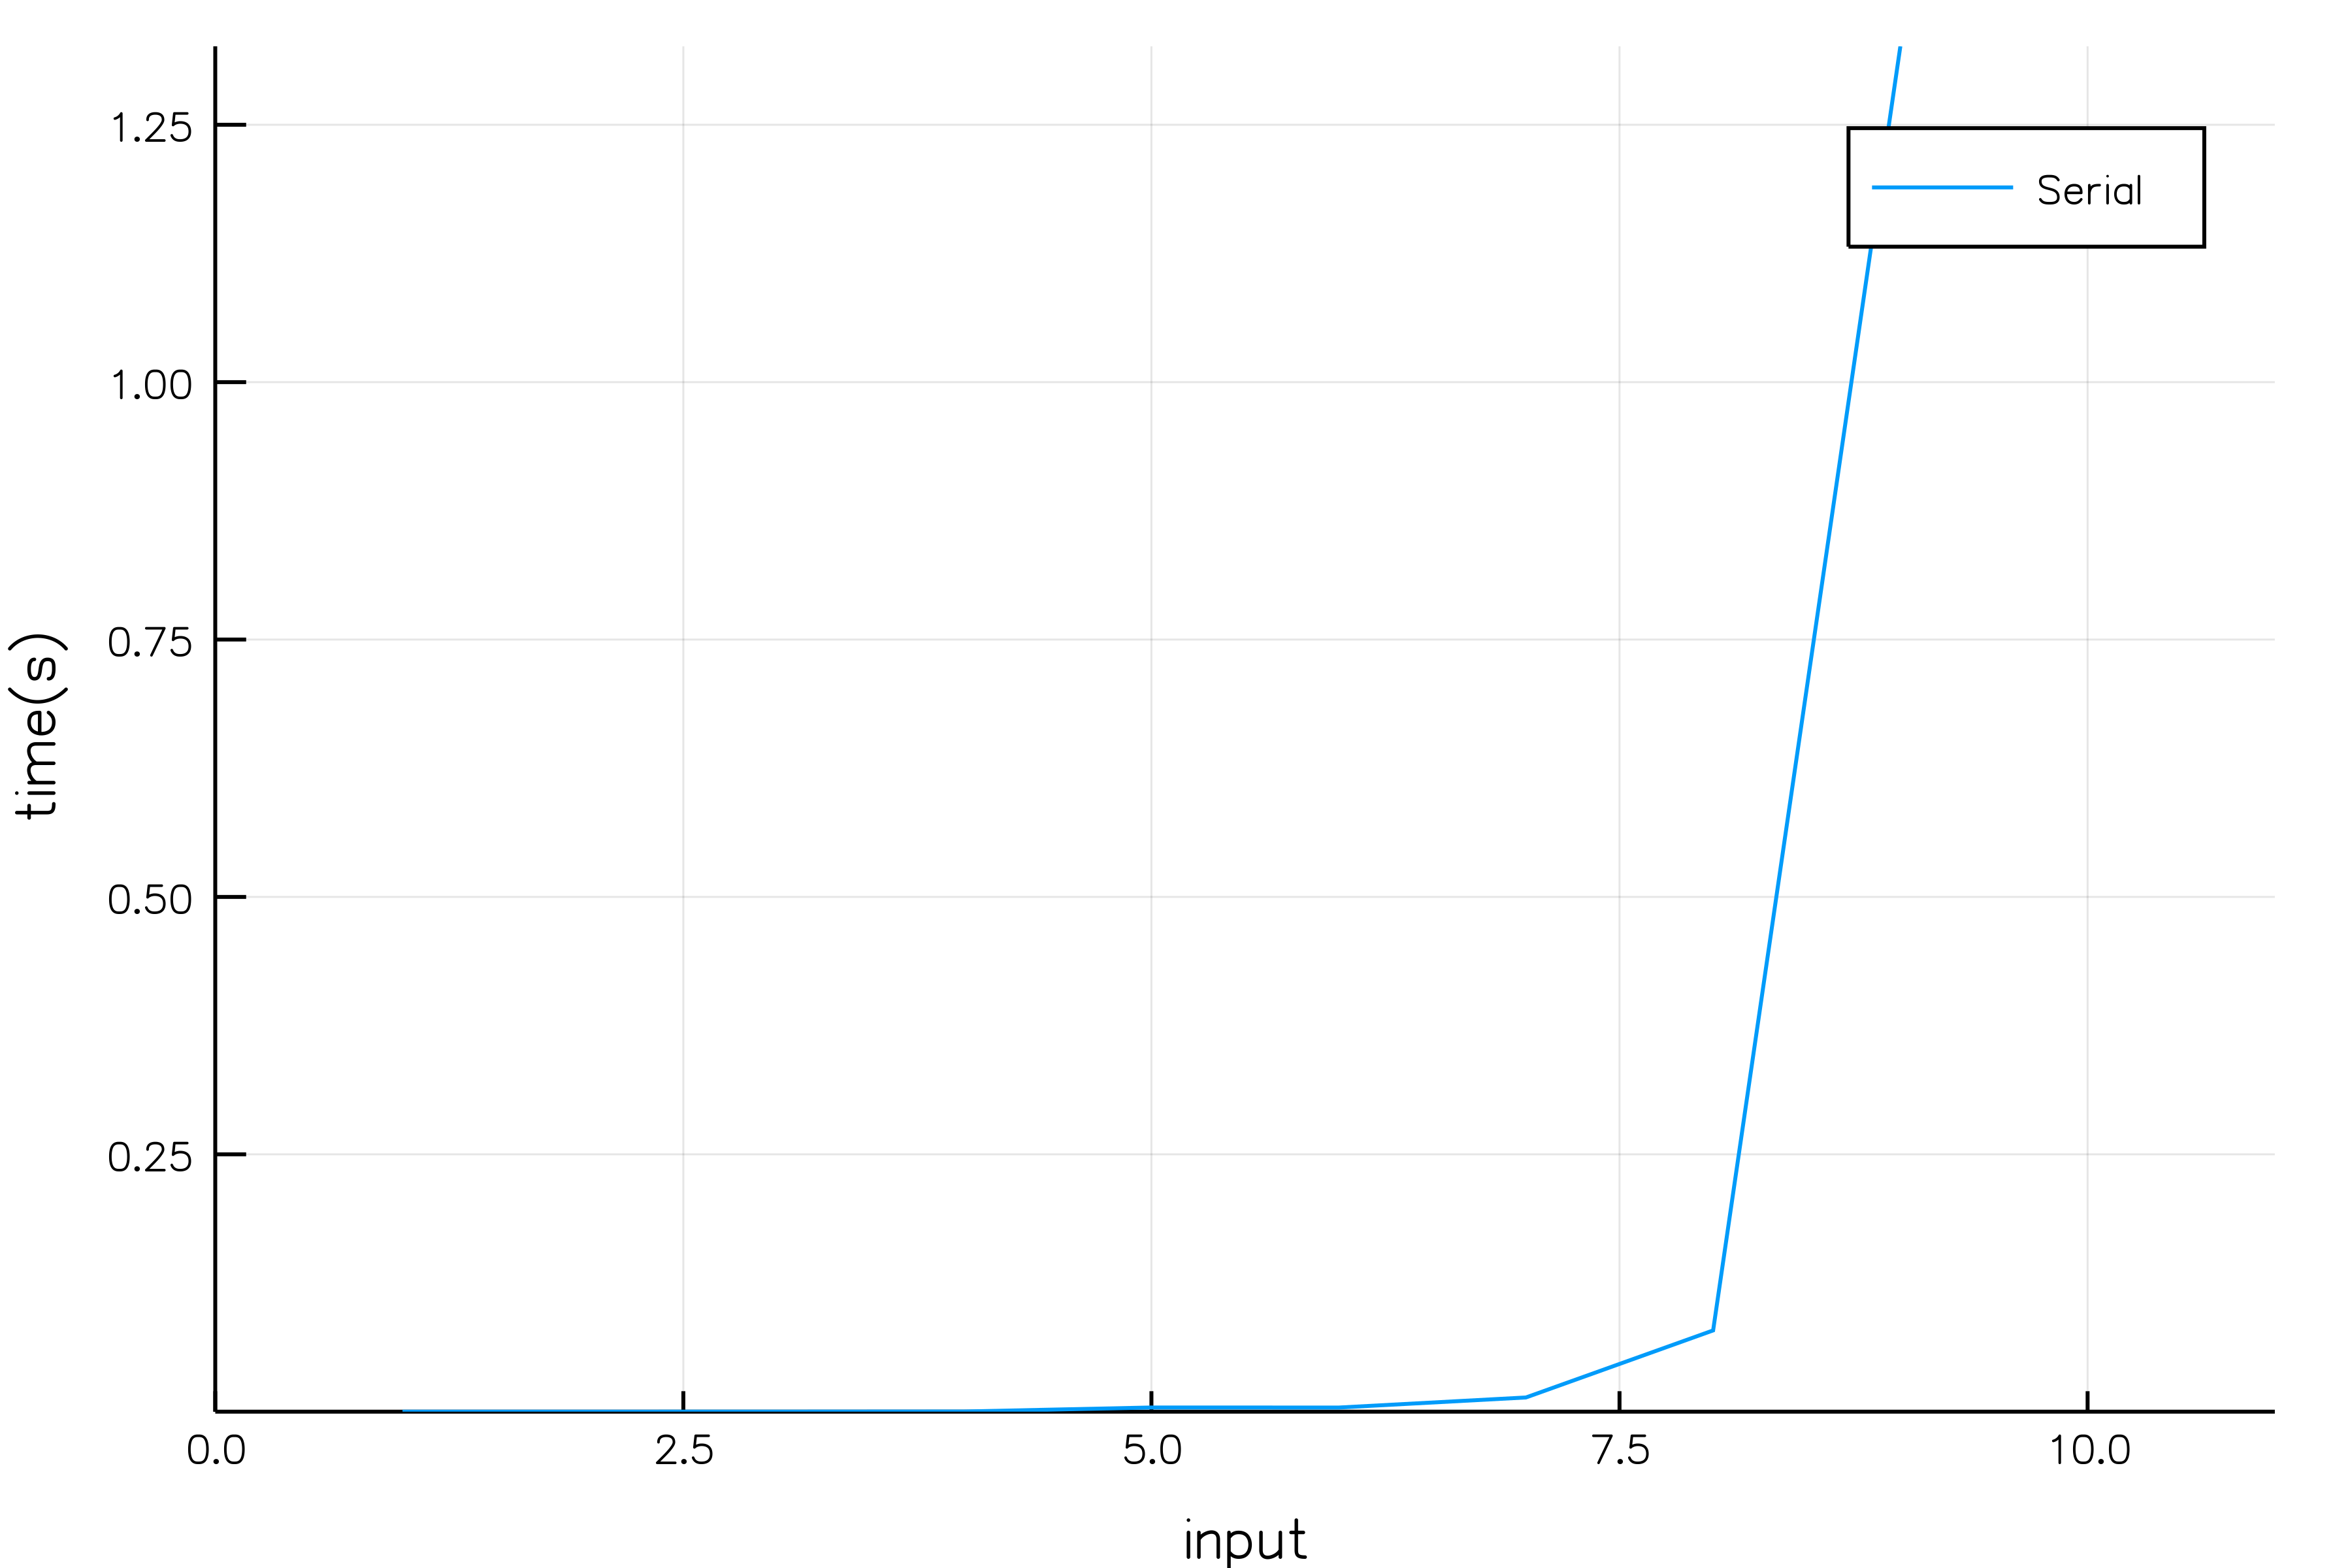
\includegraphics[scale=0.060]{struct.png}
}
\subfloat[Parallel]{%
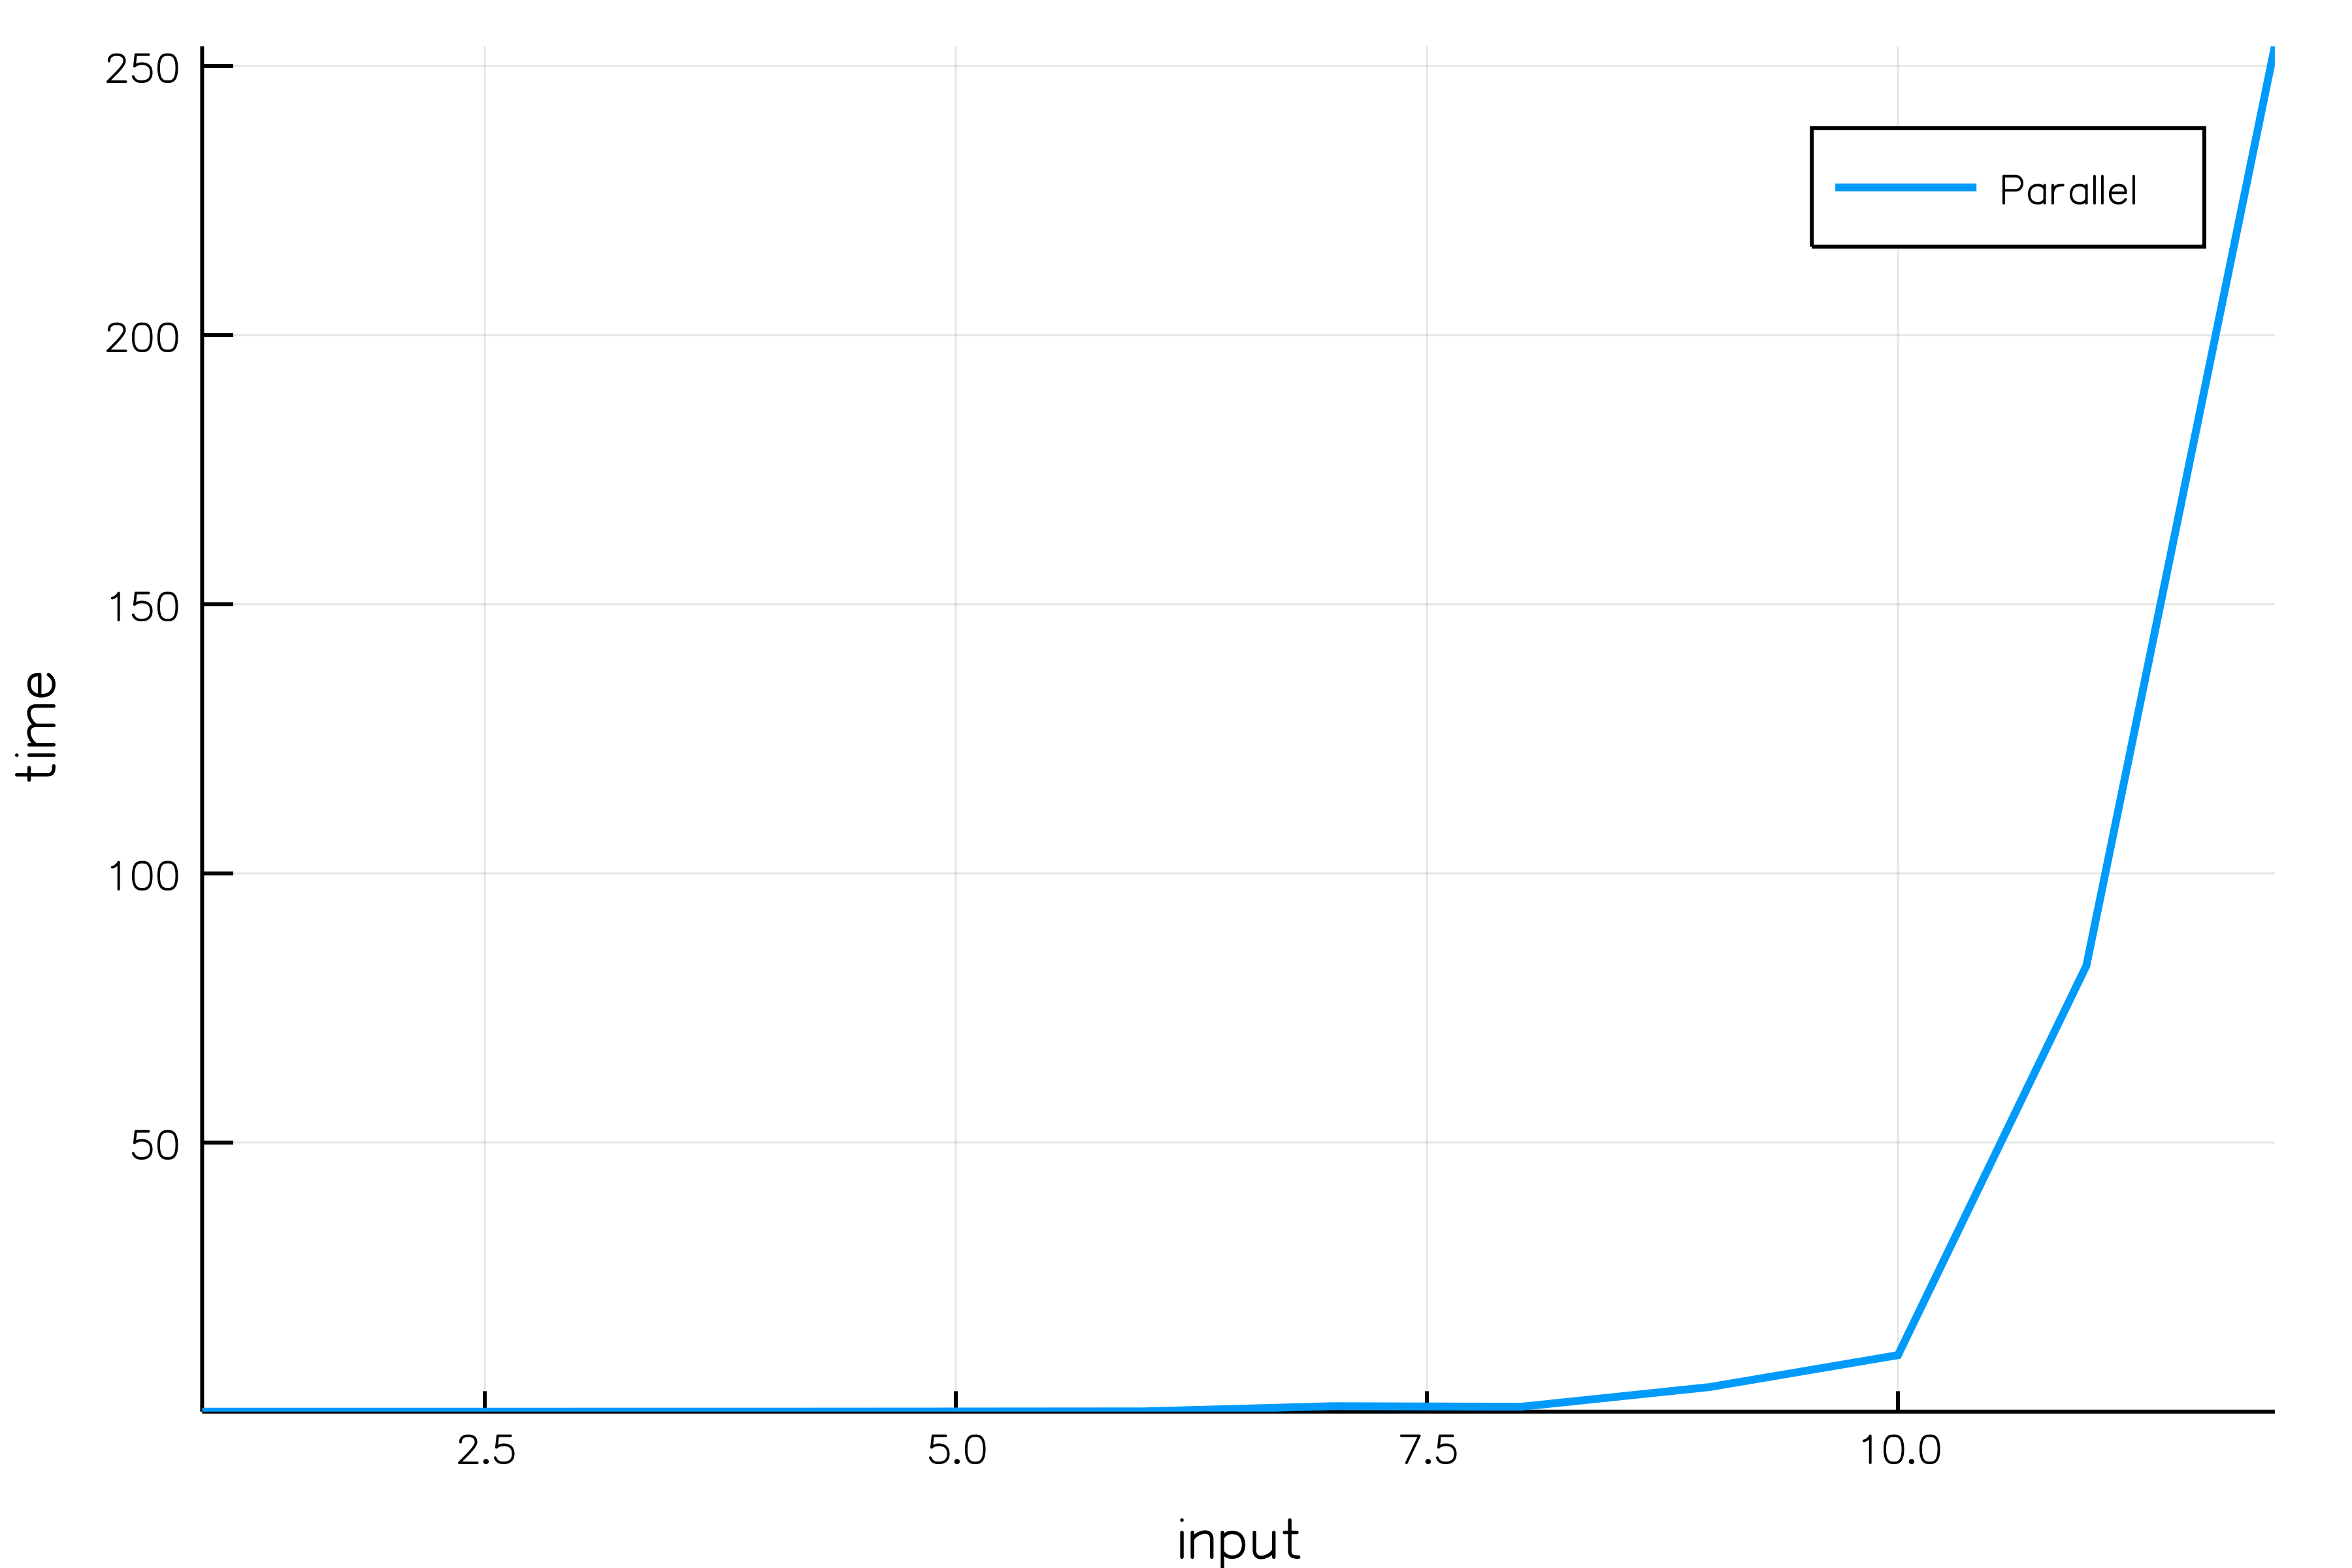
\includegraphics[scale=0.060]{pstruct.png}
}
\caption{Execution time of function Struct on Tesla}
\end{figure*}
%__________________________________________________________________________________________________________________________
\newpage

\framebox[42em][c]{Compare}

\begin{Verbatim}[fontsize=\footnotesize]
yc=[y,yp]
pc=plot(yc,label=["Serial" "Parallel"])
\end{Verbatim}
\begin{figure}[!h]
\centering
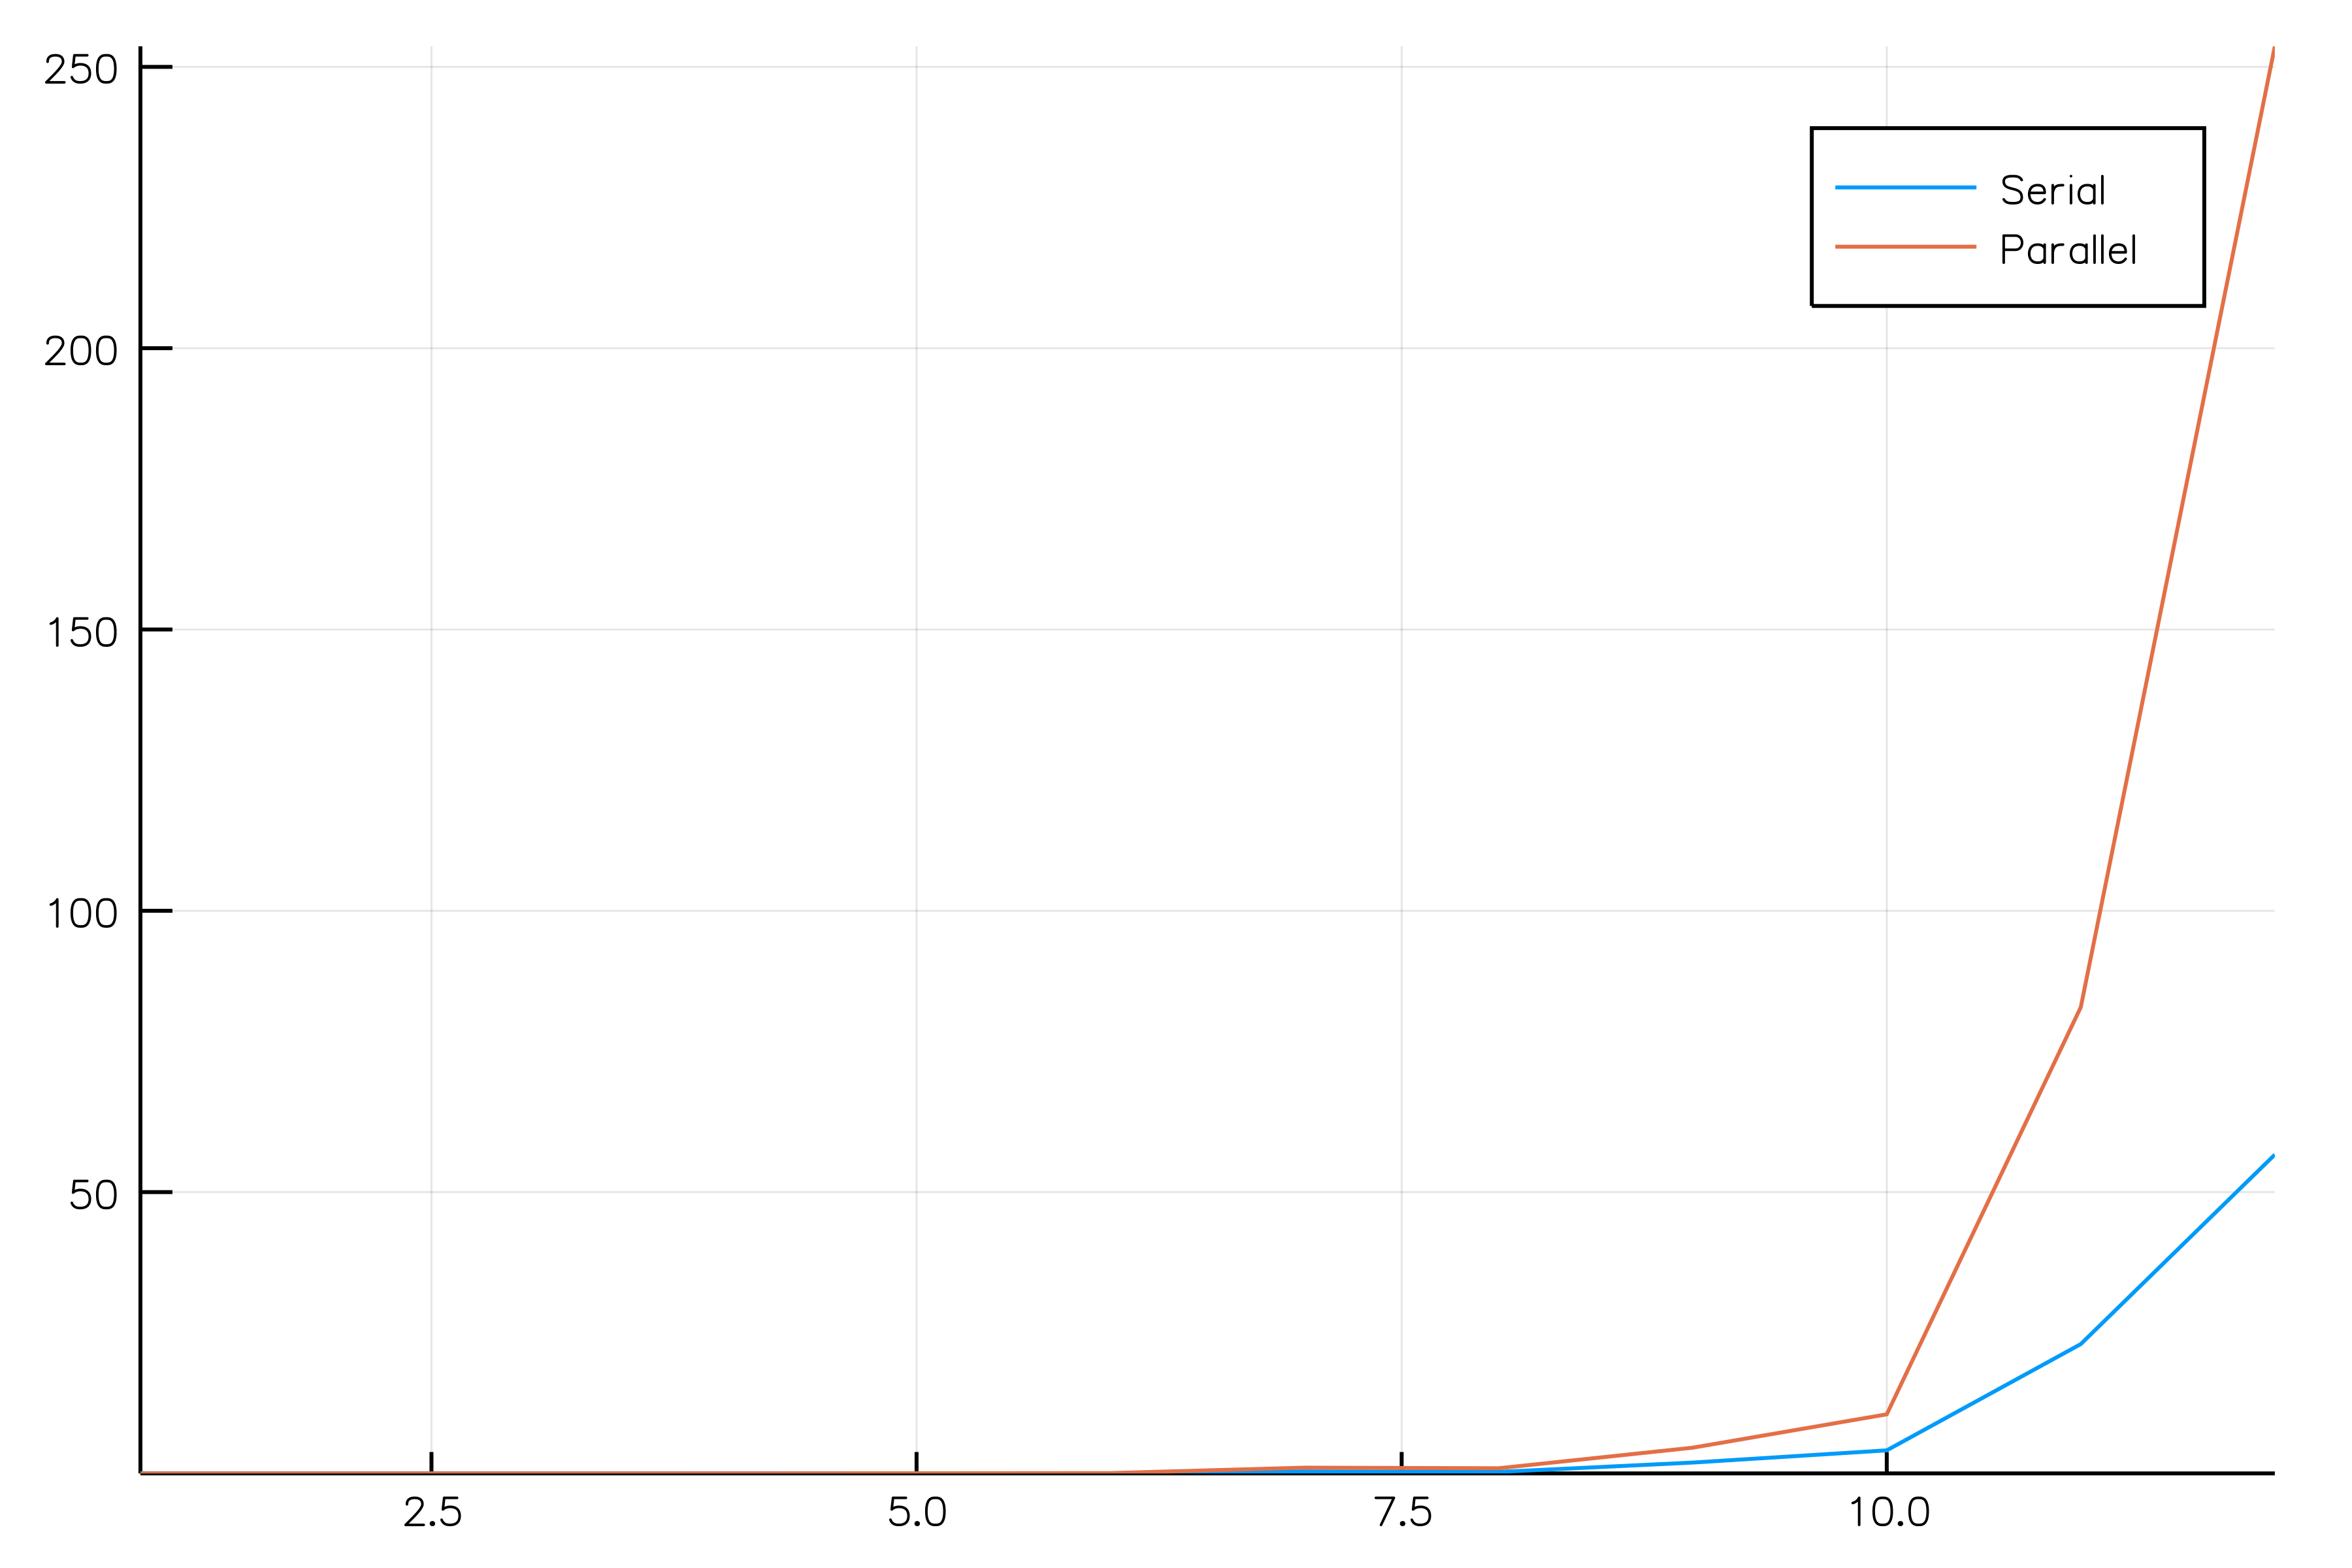
\includegraphics[scale=0.08]{compstruct.png}
\caption{Compared execution time of function Struct  on Tesla}
\end{figure}

\newpage

%__________________________________________________________________________________________________________________________

\subsection{embedTraversal}
\subsubsection{Conversion}
\framebox[5em][c]{\textbf{\normalsize Python}}
\begin{Verbatim}[fontsize=\footnotesize]
def embedTraversal(cloned, obj,n,suffix):
  for i in range(len(obj)):
    if isinstance(obj[i],Model):
      cloned.body += [obj[i]]
    elif (isinstance(obj[i],tuple) or isinstance(obj[i],list)) and (len(obj[i])==2):
      V,EV = obj[i]
      V = [v+n*[0.0] for v in V]
      cloned.body  += [(V,EV)]
    elif (isinstance(obj[i],tuple) or isinstance(obj[i],list)) and (len(obj[i])==3):
      V,FV,EV = obj[i]
      V = [v+n*[0.0] for v in V]
      cloned.body  += [(V,FV,EV)]
    elif isinstance(obj[i],Mat):
      mat = obj[i]
      d,d = mat.shape
      newMat = scipy.identity(d+n*1)
      for h in range(d-1):
	for k in range(d-1):
	  newMat[h,k] = mat[h,k]
	newMat[h,d-1+n*1] = mat[h,d-1]
	cloned.body  +=  [newMat.view(Mat)]
    elif isinstance(obj[i],Struct):
      newObj = Struct()
      newObj.box = hstack((obj[i].box, [n*[0],n*[0]]))
      newObj.name = obj[i].name+suffix
      newObj.category = obj[i].category
      cloned.body +=[embedTraversal(newObj, obj[i], n, suffix)]
    return cloned
\end{Verbatim}
\framebox[5em][c]{\textbf{\normalsize Julia}}
\begin{Verbatim}[fontsize=\footnotesize]
function embedTraversal(cloned,obj,n,suffix)
  for i in range(1,len(obj))
    if isa(obj.body[i],Matrix)
      mat=obj.body[i]
      d,d=size(mat)
      newMat=eye(d+n*1)
      for h in range(1,d-1)
	for k in range(1,d-1)
	  newMat[h,k]=mat[h,k]
	end
	newMat[h,d-1+n*1]=mat[h,d-1]
      end
      append!(cloned.body,newMat)
    elseif (isa(obj.body[i],Tuple) ||isa(obj.body[i],Array))&&length(obj.body[i])==3 
      V,FV,EV=obj.body[i]
      dimadd=fill([0.0],n)
      for k in dimadd
	for v in V
	  append!(v,k)
	end
      end
      append!(cloned.body,[(V,FV,EV)])
    elseif (isa(obj.body[i],Tuple) ||isa(obj.body[i],Array))&&length(obj.body[i])==2
      V,EV=deepcopy(obj.body[i])
      dimadd=fill([0.0],n)
      for k in dimadd
	for v in V
	  append!(v,k)
	end
      end
      append!(cloned.body,[(V,EV)])
    elseif isa(obj.body[i],Struct)
      newObj=Struct()
      newObj.box=hcat((obj.body[i].box,[fill([0],n),fill([0],n)]))
      newObj.category=obj.body[i].category
      append!(cloned.body,embedTraversal(newObj,obj.body[i],n,suffix))
    end
  end
  return cloned
end
\end{Verbatim}
\subsubsection{Parallelization}
\begin{Verbatim}[fontsize=\footnotesize]
@everywhere function pembedTraversal(cloned,obj,n,suffix)
  for i in range(1,len(obj))
    if (isa(obj.body[i],Matrix) || isa(obj.body[i],SharedArray))
      mat=obj.body[i]
      d,d=size(mat)
      newMat=eye(d+n*1)
      @sync begin
	for h in range(1,d-1)
	  @async begin
	    for k in range(1,d-1)
	      newMat[h,k]=mat[h,k]
	    end
	  end
	  newMat[h,d-1+n*1]=mat[h,d-1]
	end
      end
      append!(cloned.body,newMat)
    elseif (isa(obj.body[i],Tuple) ||isa(obj.body[i],Array))&& length(obj.body[i])==2 
      V,EV=deepcopy(obj.body[i])
      dimadd=fill([0.0],n)
      @sync begin
	for k in dimadd
	  @async begin
	    for v in V
	      append!(v,k)
	    end
	  end
	end
      end
      append!(cloned.body,[(V,EV)])
    elseif (isa(obj.body[i],Tuple) ||isa(obj.body[i],Array))&&length(obj.body[i])==3
      V,FV,EV=obj.body[i]
      dimadd=fill([0.0],n)
      @sync begin
	for k in dimadd
	  @async begin
	    for v in V
	      append!(v,k)
	    end
	  end
	end
      end
      append!(cloned.body,[(V,FV,EV)])
    elseif isa(obj.body[i],pStruct)
      newObj=pStruct()
      @async begin
	newObj.box=hcat((obj.body[i].box,[fill([0],n),fill([0],n)]))
	newObj.category=obj.body[i].category
	append!(cloned.body,embedTraversal(newObj,obj.body[i],n,suffix))
      end
    end
  end
  return cloned
end
\end{Verbatim}
\subsubsection{Unit-Test}
\framebox[42em][c]{Serial Tests}
\begin{Verbatim}[fontsize=\footnotesize]
square=([[0,0],[0,1],[1,0],[1,1]],[[0,1,2,3]])
x=Struct([square])

@testset "embedTraversal Tests" begin
  @test length(embedTraversal(deepcopy(x),deepcopy(x),1,"New").body[2][1][1])==
  length(x.body[1][1][1])+1
  #in this case n=1, but generally:
  # length(length(embedTraversal(x,x,1,"New")=length(x.body[1][1][1])+n
  @test length(embedTraversal(deepcopy(x),deepcopy(x),3,"New").body[2][1][1])==
  length(x.body[1][1][1])+3
  @test typeof(embedTraversal(deepcopy(x),deepcopy(x),1,"New"))==Struct	
end
\end{Verbatim}
\framebox[42em][c]{Parallel Tests}
\begin{Verbatim}[fontsize=\footnotesize]
square=([[0,0],[0,1],[1,0],[1,1]],[[0,1,2,3]])
x=pStruct([square])

@testset "pembedTraversal Tests" begin
  @test length(pembedTraversal(deepcopy(x),deepcopy(x),1,"New").body[2][1][1])==
  length(x.body[1][1][1])+1
  #in this case n=1, but generally:
  #length(length(embedTraversal(x,x,1,"New")=length(x.body[1][1][1])+n
  @test length(pembedTraversal(deepcopy(x),deepcopy(x),3,"New").body[2][1][1])==
  length(x.body[1][1][1])+3
  @test typeof(pembedTraversal(deepcopy(x),deepcopy(x),1,"New"))==pStruct	
end
\end{Verbatim}
\subsubsection{Results}
\textbf{Execution time on Tesla}
\begin{Verbatim}[fontsize=\footnotesize]
input=[1,10,20,50,10^2,2*10^2,5*10^2,10^3,2*10^3]
function timeEmbedTraversal(model,input)
  t=Array{Float64}(length(input))
  pt=Array{Float64}(length(input))
  for i in range(1,length(input))
    structo=addn2D(input[i],model)
    pstructo=pStruct(structo.body)
    cloned=Struct()
    cloned.box=hcat((structo.box,[fill([0],10),fill([0],10)]))
    cloned.name=string(object_id(cloned))
    cloned.category=structo.category
    cloned.dim=structo.dim+10
    pcloned=pStruct()
    pcloned.box=hcat((pstructo.box,[fill([0],10),fill([0],10)]))
    pcloned.name=string(object_id(pcloned))
    pcloned.category=pstructo.category
    pcloned.dim=pstructo.dim+10
    embedTraversal(cloned,structo,10,"New")
    pembedTraversal(pcloned,pstructo,10,"New")
    t[i]=@elapsed embedTraversal(cloned,structo,10,"New")
    pt[i]=@elapsed pembedTraversal(pcloned,pstructo,10,"New")
  end
  return t,pt
end
y,yp=timeEmbedTraversal(square,input)
p=plot(input,y,xaxis="input",yaxis="time",xlims=(0,length(input)+1),
       ylims=(0,maximum(y)+0.5), label=["Serial"],lw=2)       
pp=plot(input,yp,xaxis="input",yaxis="time",xlims=(0,length(input)+1),
       ylims=(0,maximum(y)+0.5),label=["Parallel"],lw=2)      
\end{Verbatim}
\begin{figure*}[!h]
\centering
\subfloat[Serial]{%
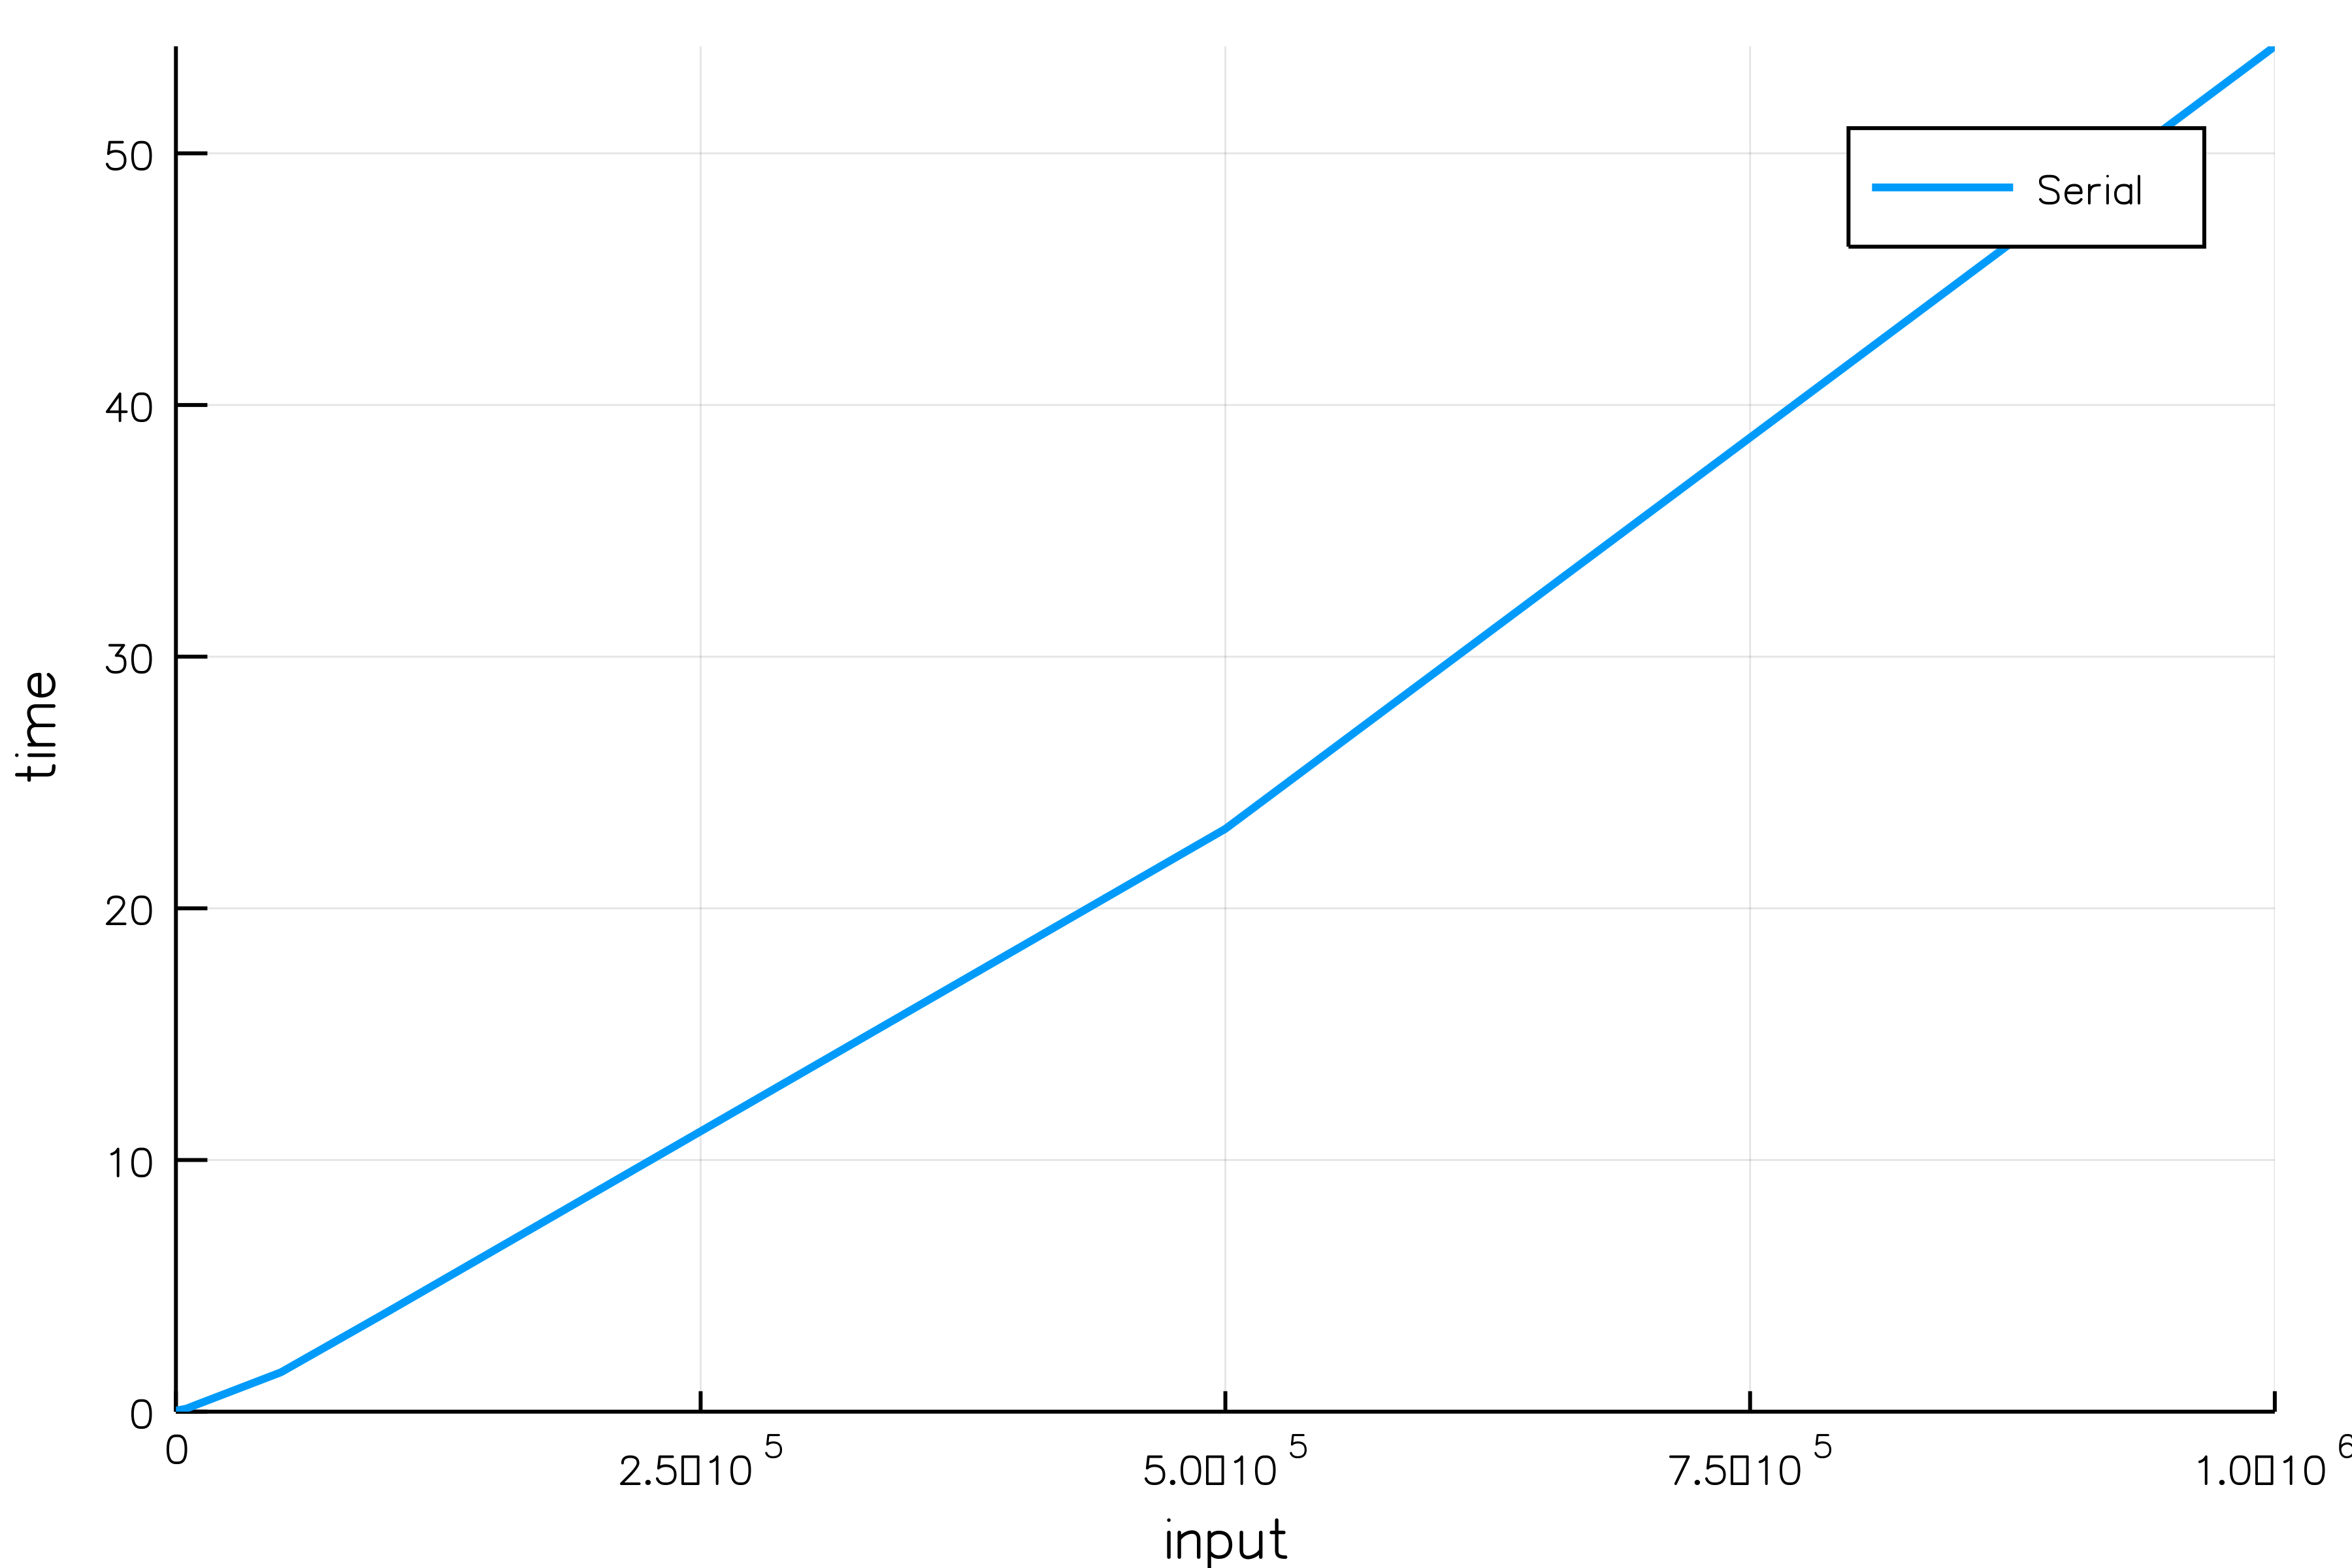
\includegraphics[scale=0.060]{embedtraversal.png}
}
\subfloat[Parallel]{%
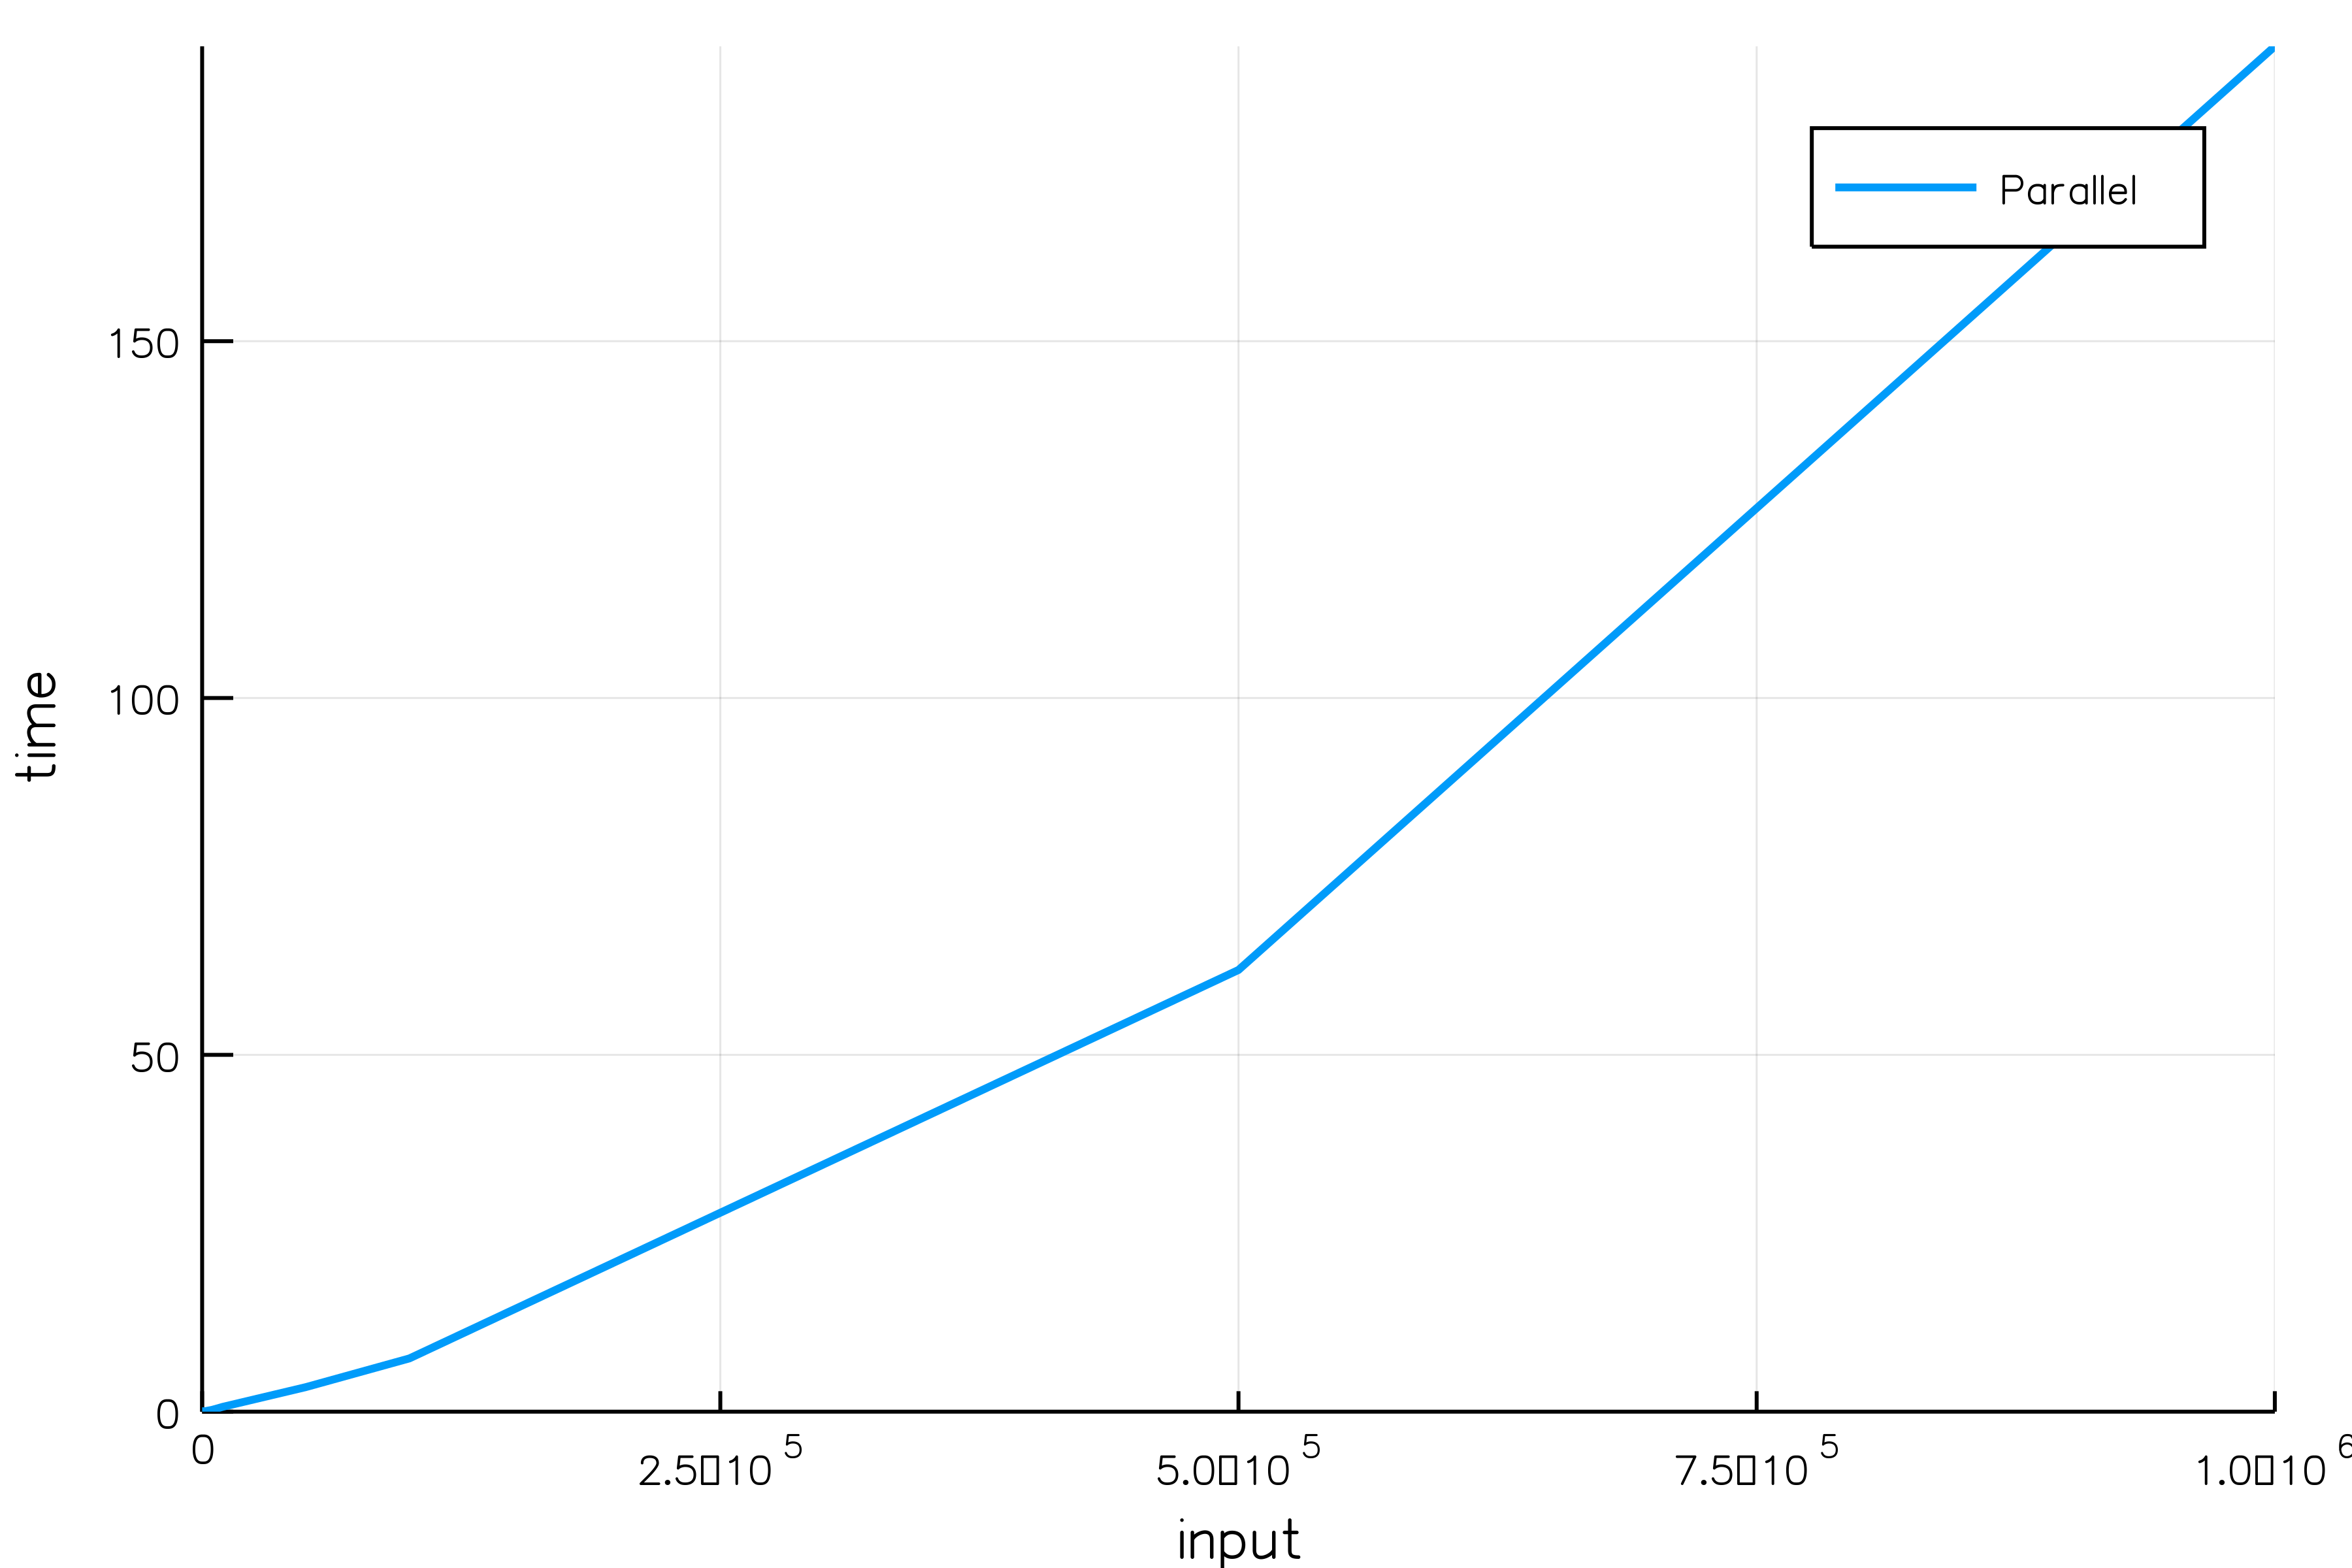
\includegraphics[scale=0.060]{pembedtraversal.png}
}
\caption{Execution time of function embedTraversal on Tesla}
\end{figure*}
\noindent \framebox[42em][c]{Compare}
\begin{Verbatim}[fontsize=\footnotesize]
yc=[y,yp]
pc=plot(input,yc,label=["Serial" "Parallel"])
\end{Verbatim}
\begin{figure}[!h]
\centering
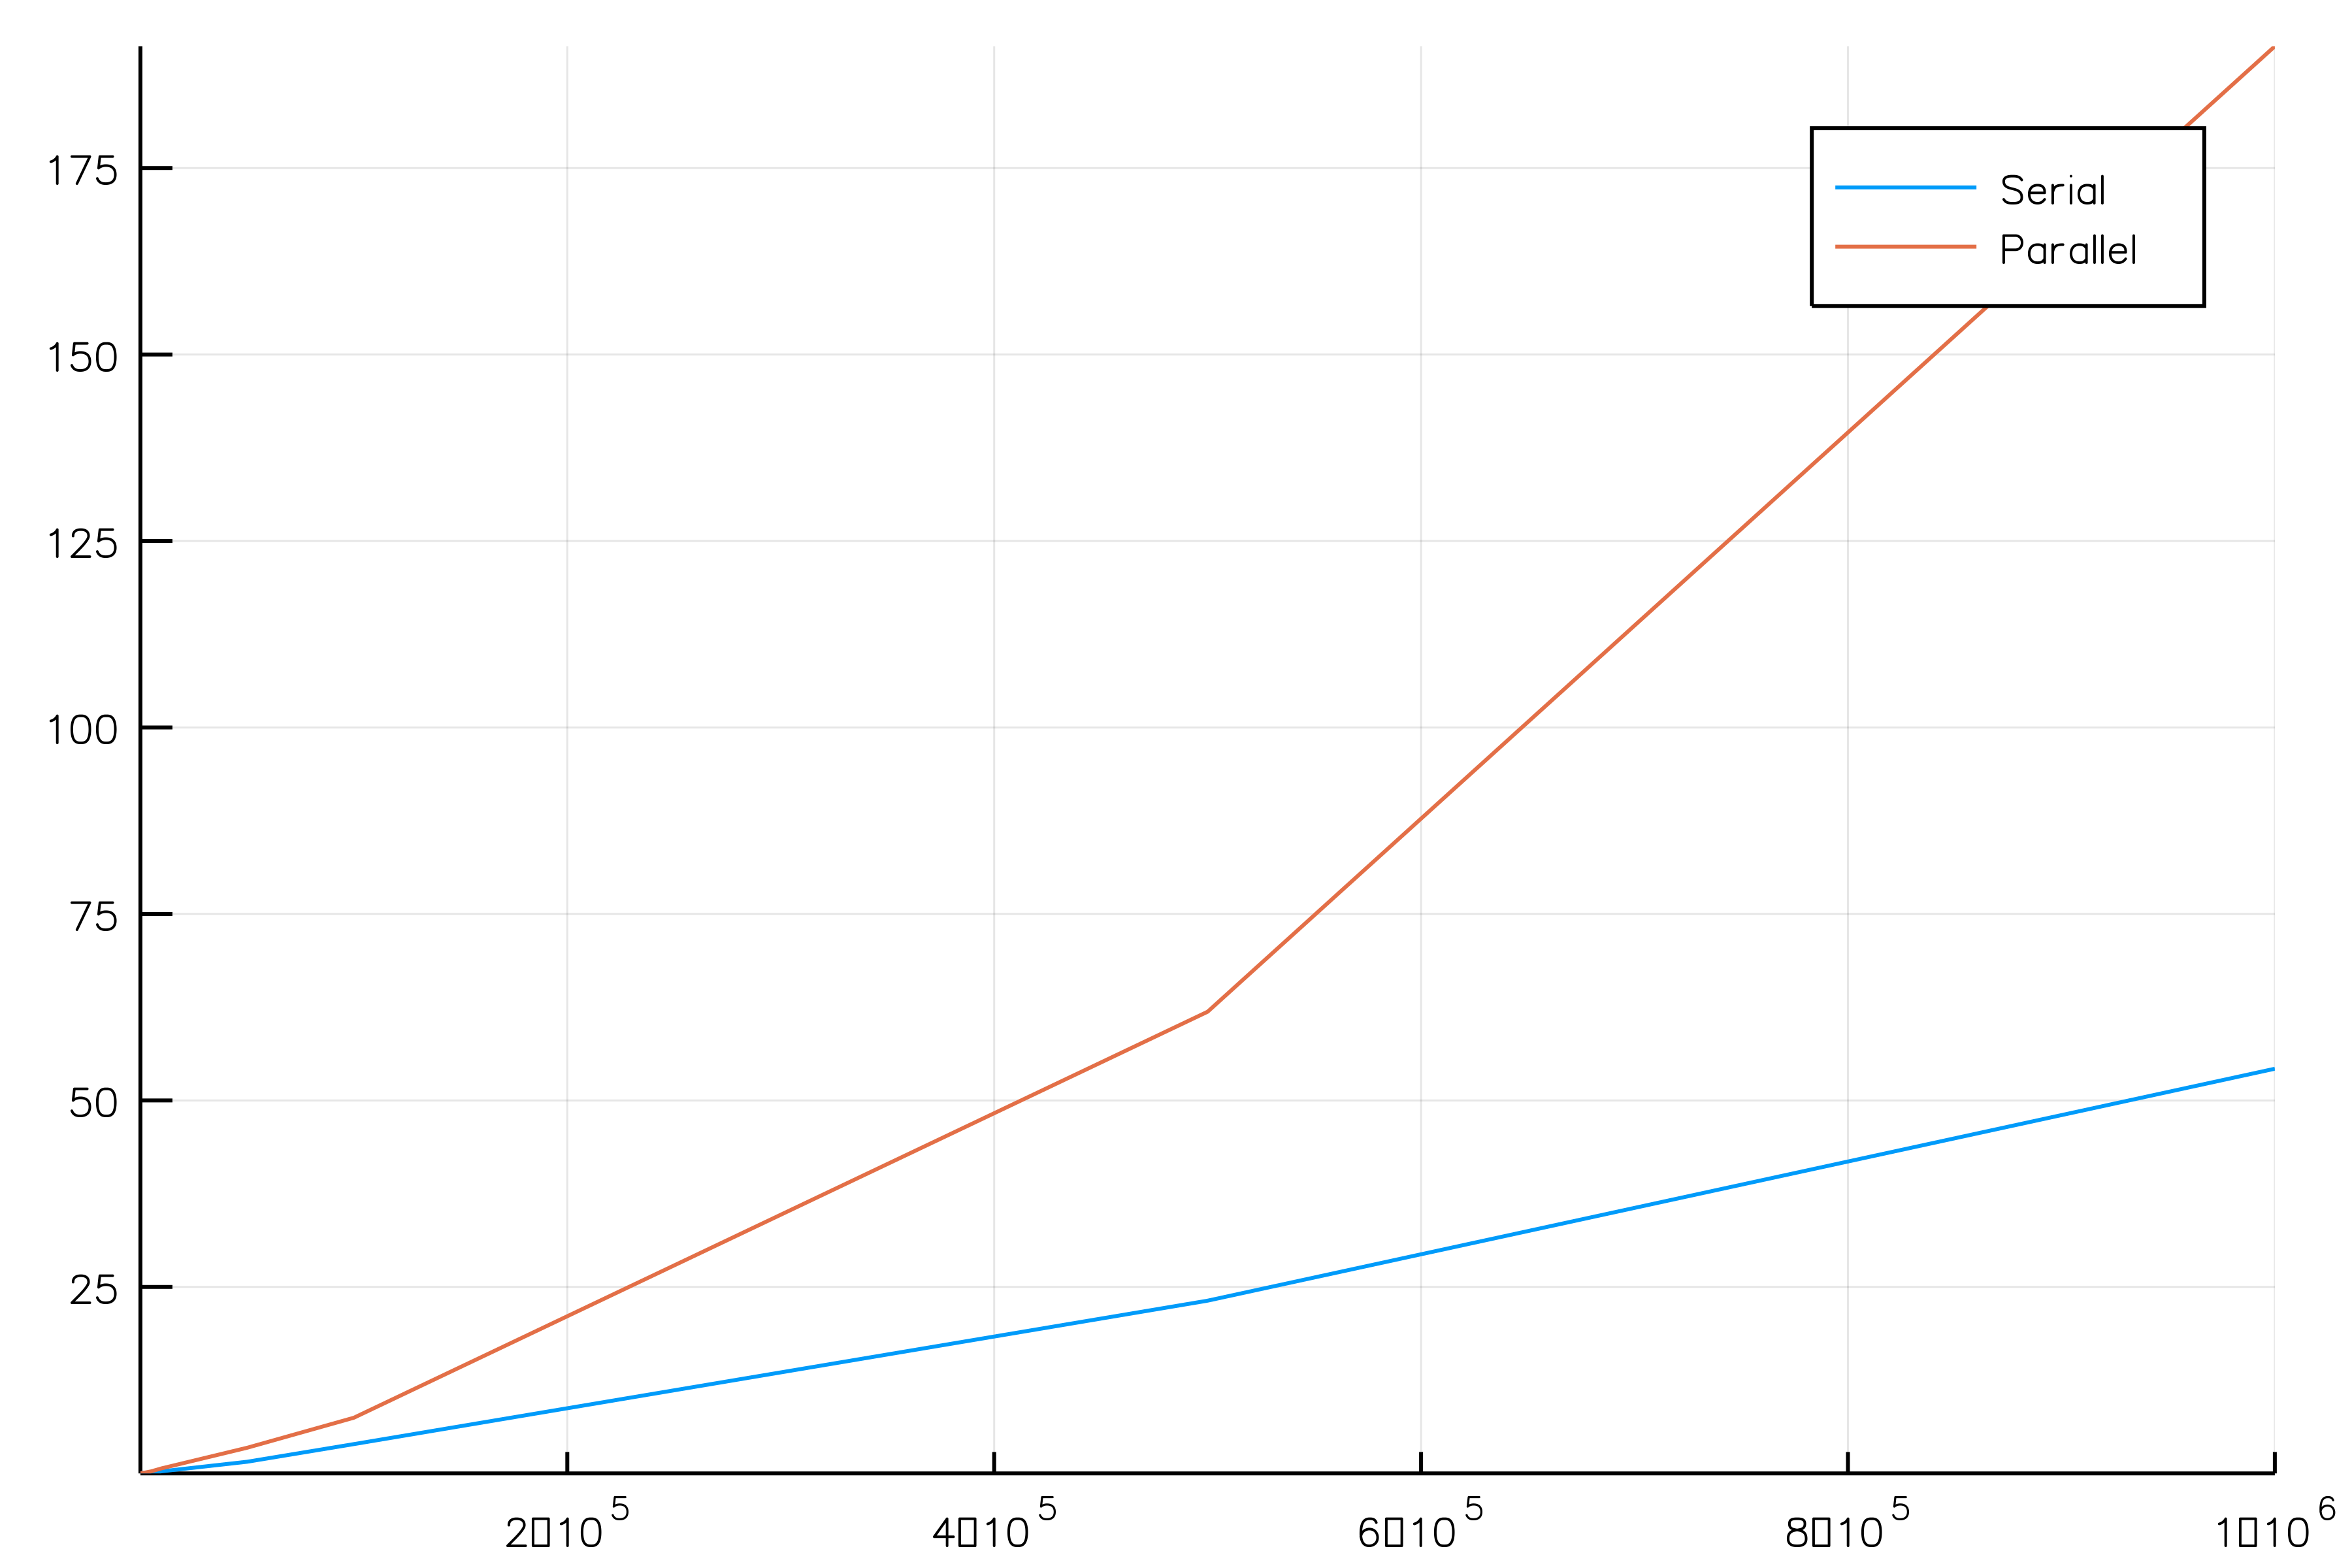
\includegraphics[scale=0.08]{compembedtraversal.png}
\caption{Compared execution time of function embedtraversal on Tesla}
\end{figure}

%__________________________________________________________________________________________________________________________
\newpage

\subsection{embedStruct}
\subsubsection{Conversion}
\framebox[5em][c]{\textbf{\normalsize Python}}
\begin{Verbatim}[fontsize=\footnotesize]

def embedStruct(n):
  def embedStruct0(struct,suffix="New"):
    if n==0:
      return struct, len(struct.box[0])
    cloned = Struct()
    cloned.box = hstack((struct.box, [n*[0],n*[0]])).tolist()
    cloned.name = str(id(cloned))  #struct.name+suffix
    cloned.category = struct.category
    cloned.dim = struct.dim + n
    cloned = embedTraversal(cloned,struct,n,suffix) 
    return cloned
  return embedStruct0
  
\end{Verbatim}
\framebox[5em][c]{\textbf{\normalsize Julia}}
\begin{Verbatim}[fontsize=\footnotesize]

function embedStruct(n)
  function embedStruct0(self,suffix="New")
    if n==0
      return self, length(self.box[1])
    end
    cloned=Struct()
    cloned.box=hcat((self.box,[fill([0],n),fill([0],n)]))
    cloned.name=string(object_id(cloned))
    cloned.category=self.category
    cloned.dim=self.dim+n
    cloned=embedTraversal(cloned,self,n,suffix)
    return cloned
 end
 return embedStruct0
end

\end{Verbatim}
\subsubsection{Parallelization}
\begin{Verbatim}[fontsize=\footnotesize]

@everywhere function pembedStruct(n)
  function pembedStruct0(self,suffix="New")
    if n==0
      return self, length(self.box[1])
    end
    cloned=pStruct()
    cloned.box=hcat((self.box,[fill([0],n),fill([0],n)]))
    cloned.name=string(object_id(cloned))
    cloned.category=self.category
    cloned.dim=self.dim+n
    cloned=pembedTraversal(cloned,self,n,suffix)
    return cloned
  end
  return pembedStruct0
end

\end{Verbatim}
\subsubsection{Unit-Test}
\framebox[42em][c]{Serial Tests}
\begin{Verbatim}[fontsize=\footnotesize]

square=([[0,0],[0,1],[1,0],[1,1]],[[0,1,2,3]])
x=Struct([square])	

@testset "embedStruct Tests" begin
  @test length(embedStruct(1)(x).body[1][1][1])==length(x.body[1][1][1])+1
  #in this case n = 1, but generally: 
  #length(embedStruct(n)(x).body[1][1][1])=length(x.body[1][1][1])+n
  @test length(embedStruct(3)(x).body[1][1][1])==length(x.body[1][1][1])+3
  @test typeof(embedStruct(1)(x))==Struct	
end

\end{Verbatim}

\framebox[42em][c]{Parallel Tests}
\begin{Verbatim}[fontsize=\footnotesize]

square=([[0,0],[0,1],[1,0],[1,1]],[[0,1,2,3]])
x=pStruct([square])

@testset "pembedStruct Tests" begin
  @test length(pembedStruct(1)(x).body[1][1][1])==length(x.body[1][1][1])+1 
  #in this case n = 1, but generally: 
  #length(embedStruct(n)(x).body[1][1][1])=length(x.body[1][1][1])+n
  @test length(pembedStruct(3)(x).body[1][1][1])==length(x.body[1][1][1])+3
  @test typeof(pembedStruct(1)(x))==pStruct	
end

\end{Verbatim}
\subsubsection{Results}

\textbf{Execution time on Tesla}
\begin{Verbatim}[fontsize=\footnotesize]
input=[1,10,20,50,10^2,2*10^2,5*10^2,10^3,2*10^3]

function timeEmbedStruct(n,model,input)
  t=Array{Float64}(length(input))
  pt=Array{Float64}(length(input))
  for i in range(1,length(input))
    structo=addn2D(input[i],model)
    pstructo=pStruct(structo.body)
    embedStruct(n)(structo)
    pembedStruct(n)(pstructo)
    t[i]=@elapsed embedStruct(n)(structo)
    pt[i]=@elapsed pembedStruct(n)(pstructo)
  end
  return t,pt
end
y,yp=timeEmbedStruct(10,square,input)

p=plot(input,y,xaxis="input",yaxis="time",xlims=(0,length(input)+1),
       ylims=(0,maximum(y)+0.5), label=["Serial"],lw=2)       
pp=plot(input,yp,xaxis="input",yaxis="time",xlims=(0,length(input)+1),
       ylims=(0,maximum(y)+0.5),label=["Parallel"],lw=2)
\end{Verbatim}
\vspace{25px}

\begin{figure*}[!h]
\centering
\subfloat[Serial]{%
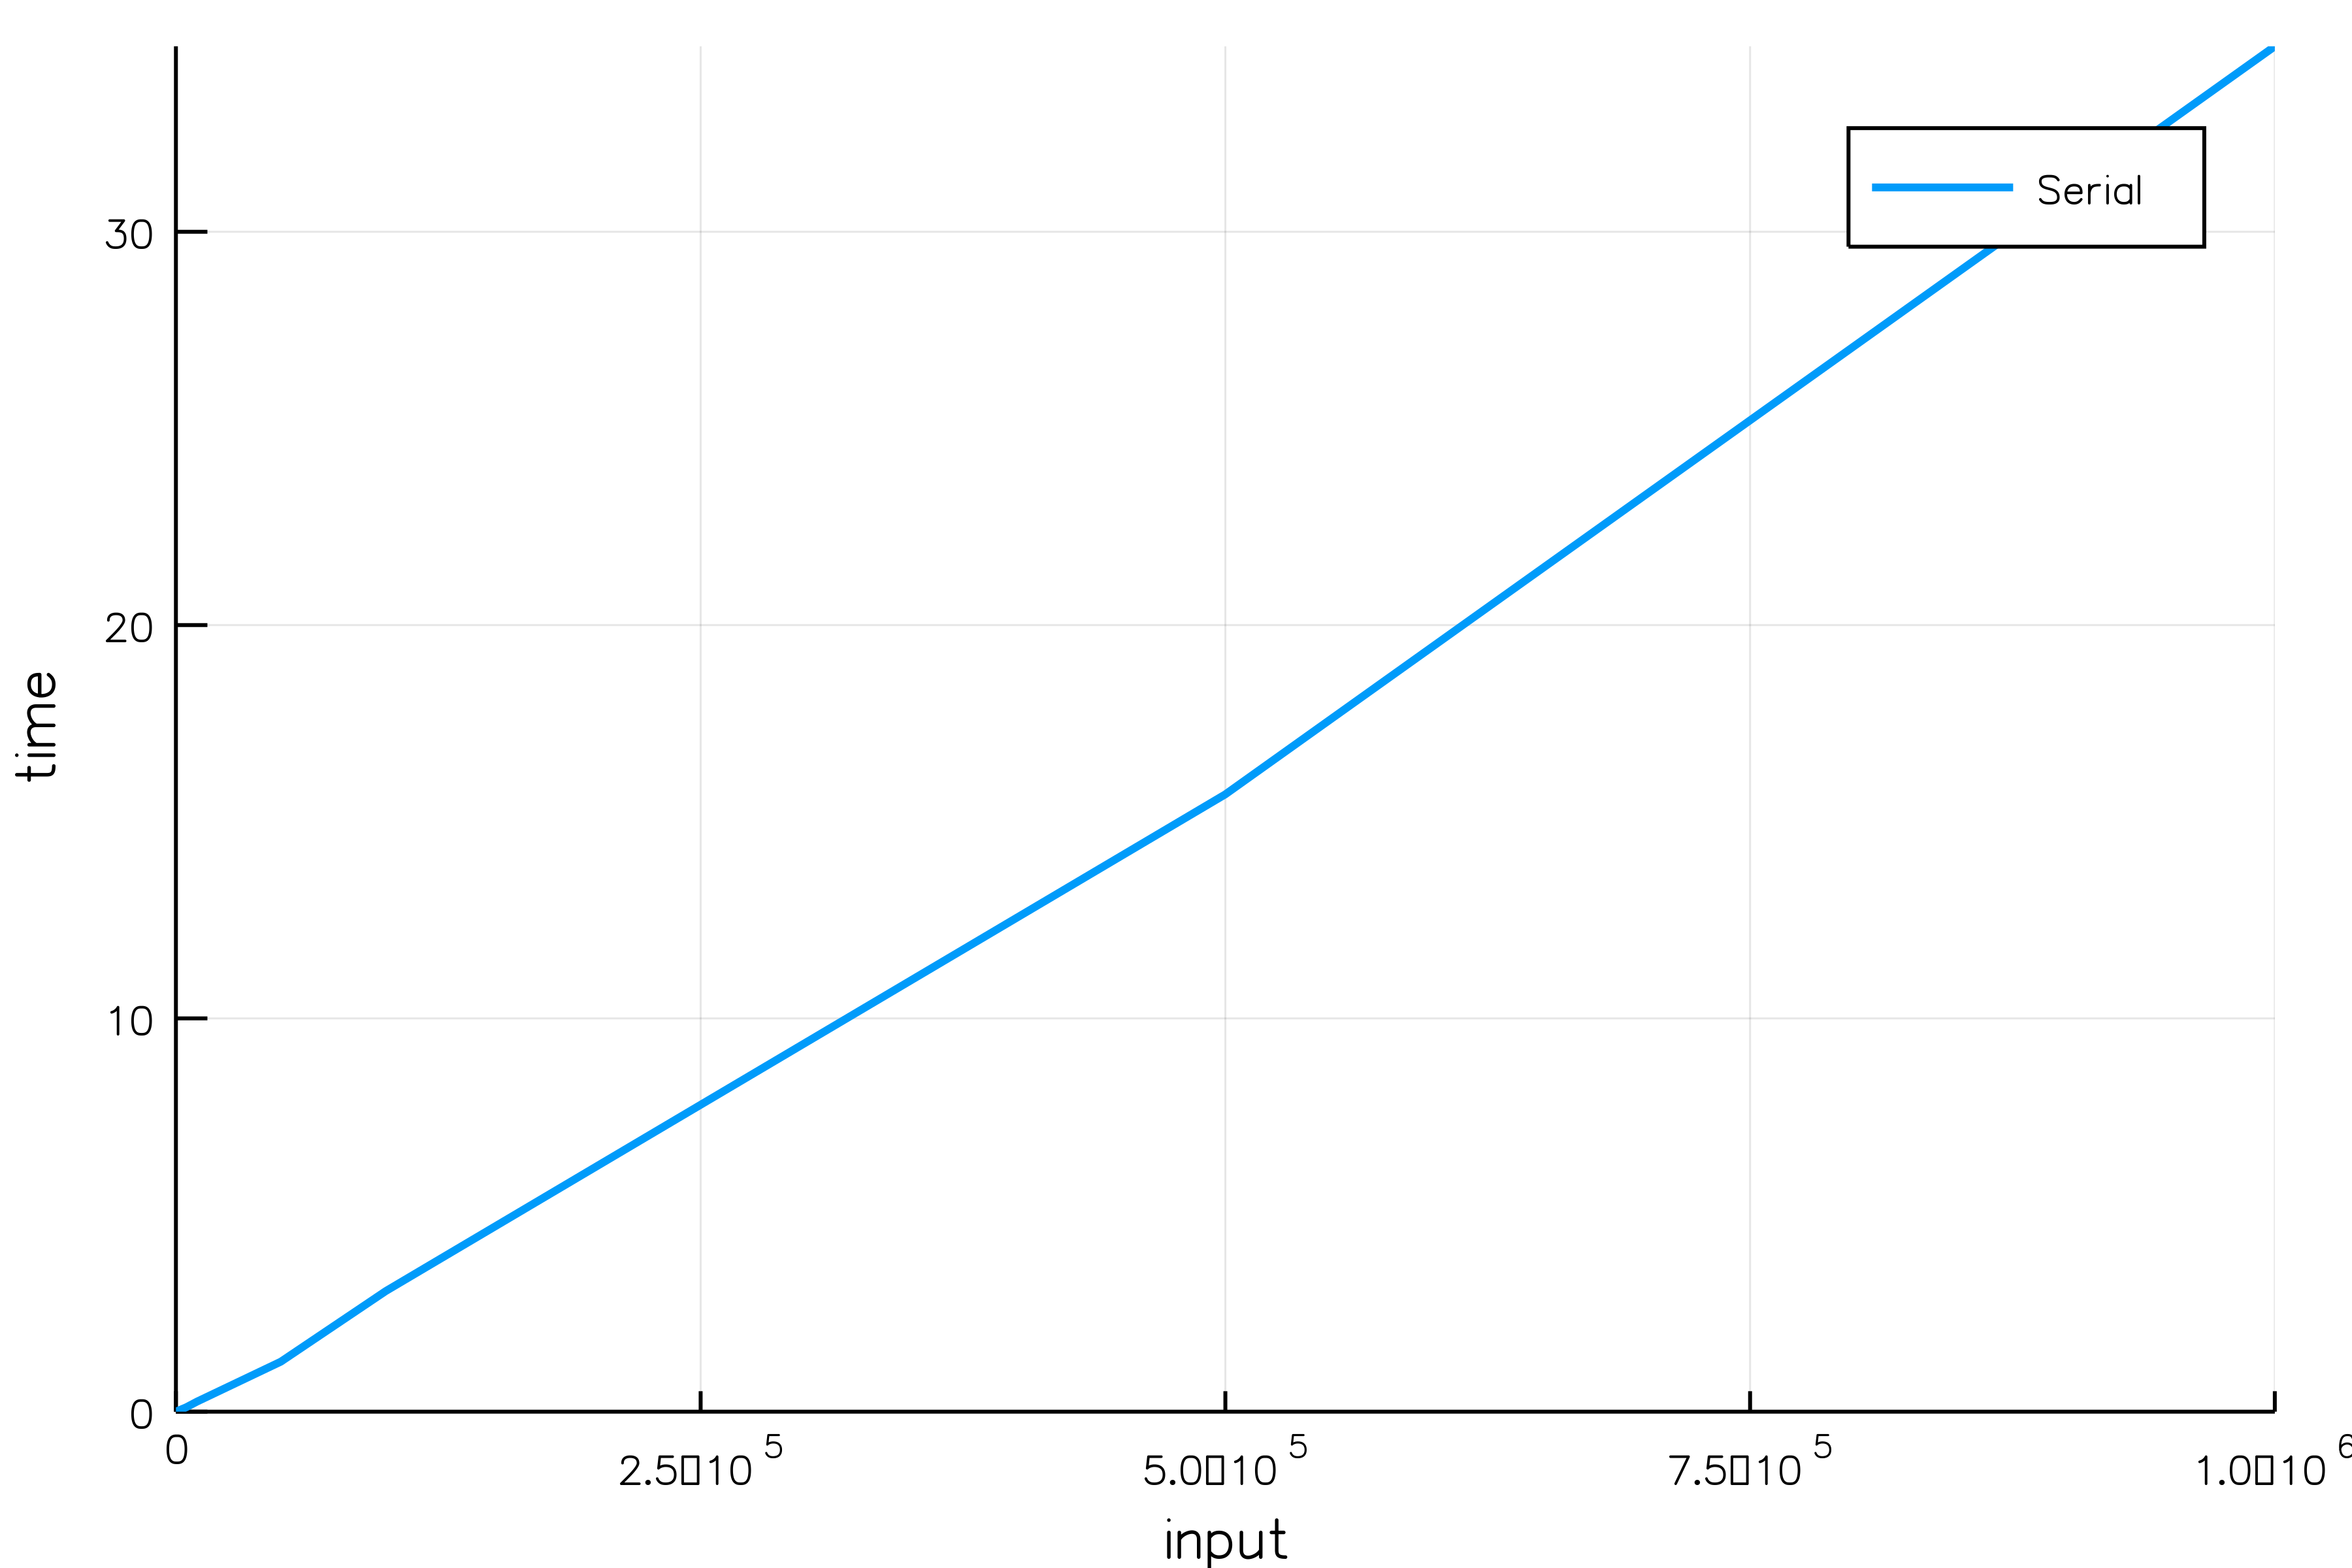
\includegraphics[scale=0.060]{embedStruct.png}
}
\subfloat[Parallel]{%
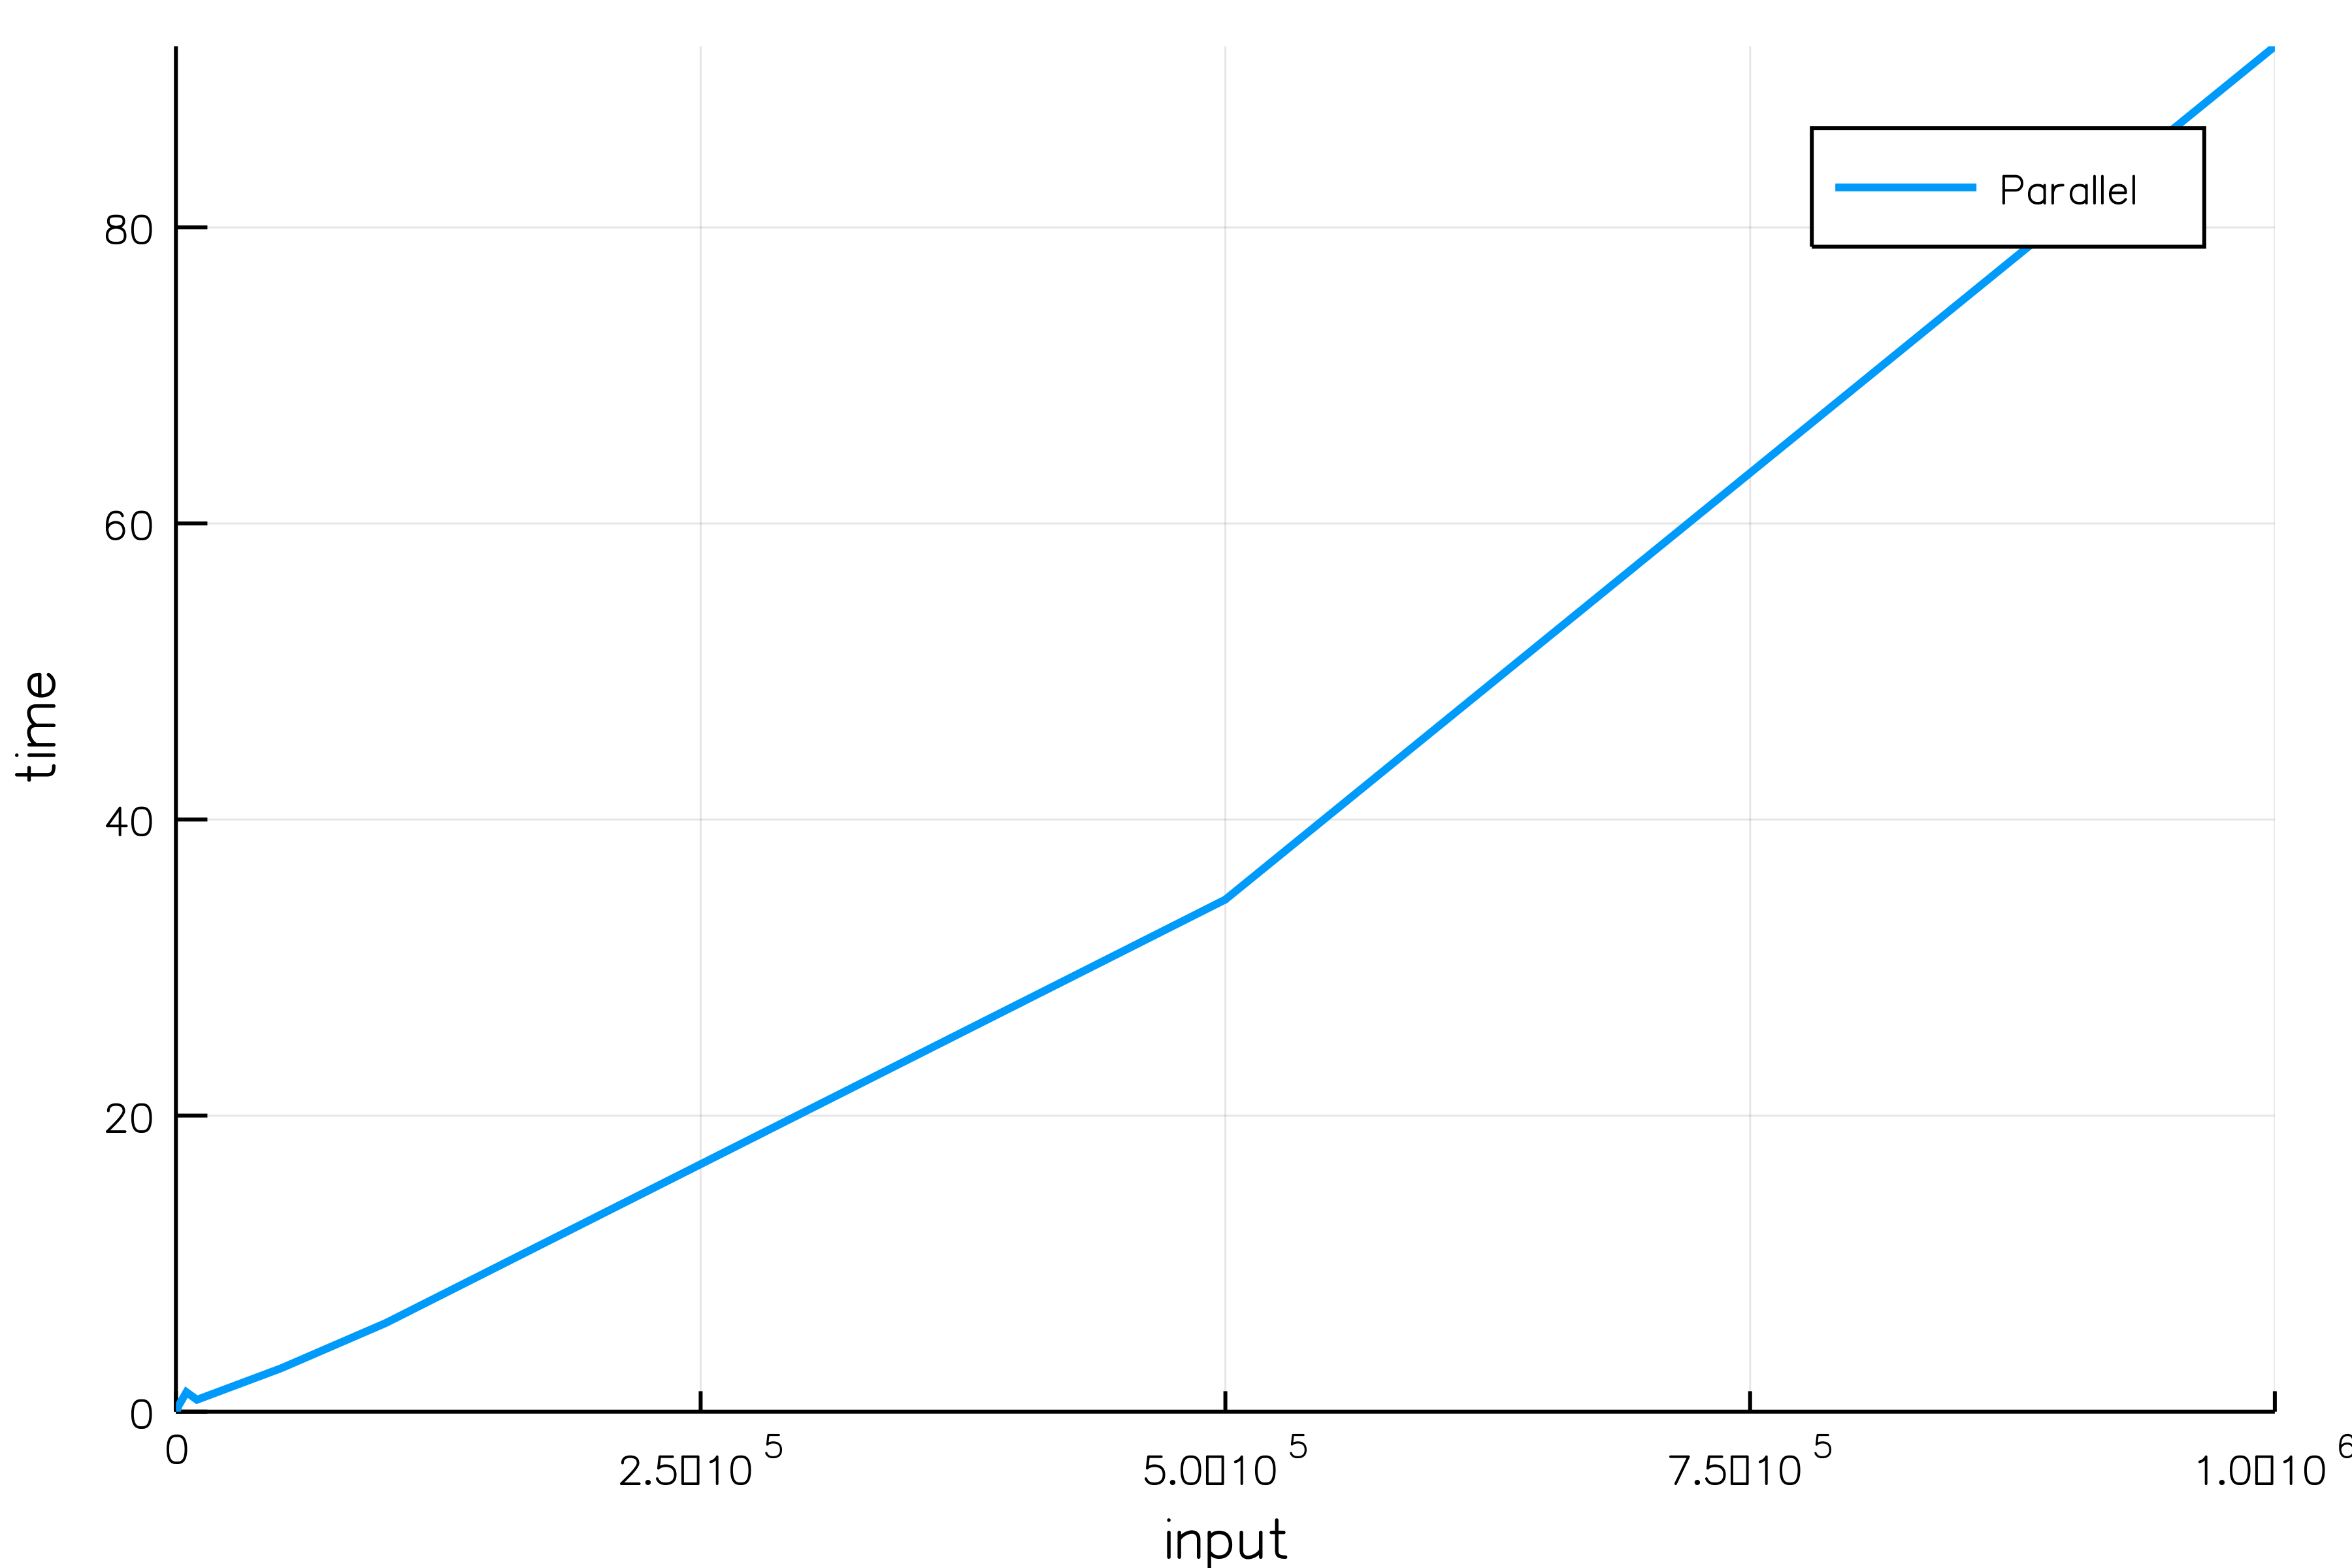
\includegraphics[scale=0.060]{pembedstruct.png}
}
\caption{Execution time of function embedStruct on Tesla}
\end{figure*}
%__________________________________________________________________________________________________________________________
\newpage

\noindent \framebox[42em][c]{Compare}
\begin{Verbatim}[fontsize=\footnotesize]
yc=[y,yp]
pc=plot(input,yc,label=["Serial" "Parallel"])
\end{Verbatim}
\begin{figure}[!h]
\centering
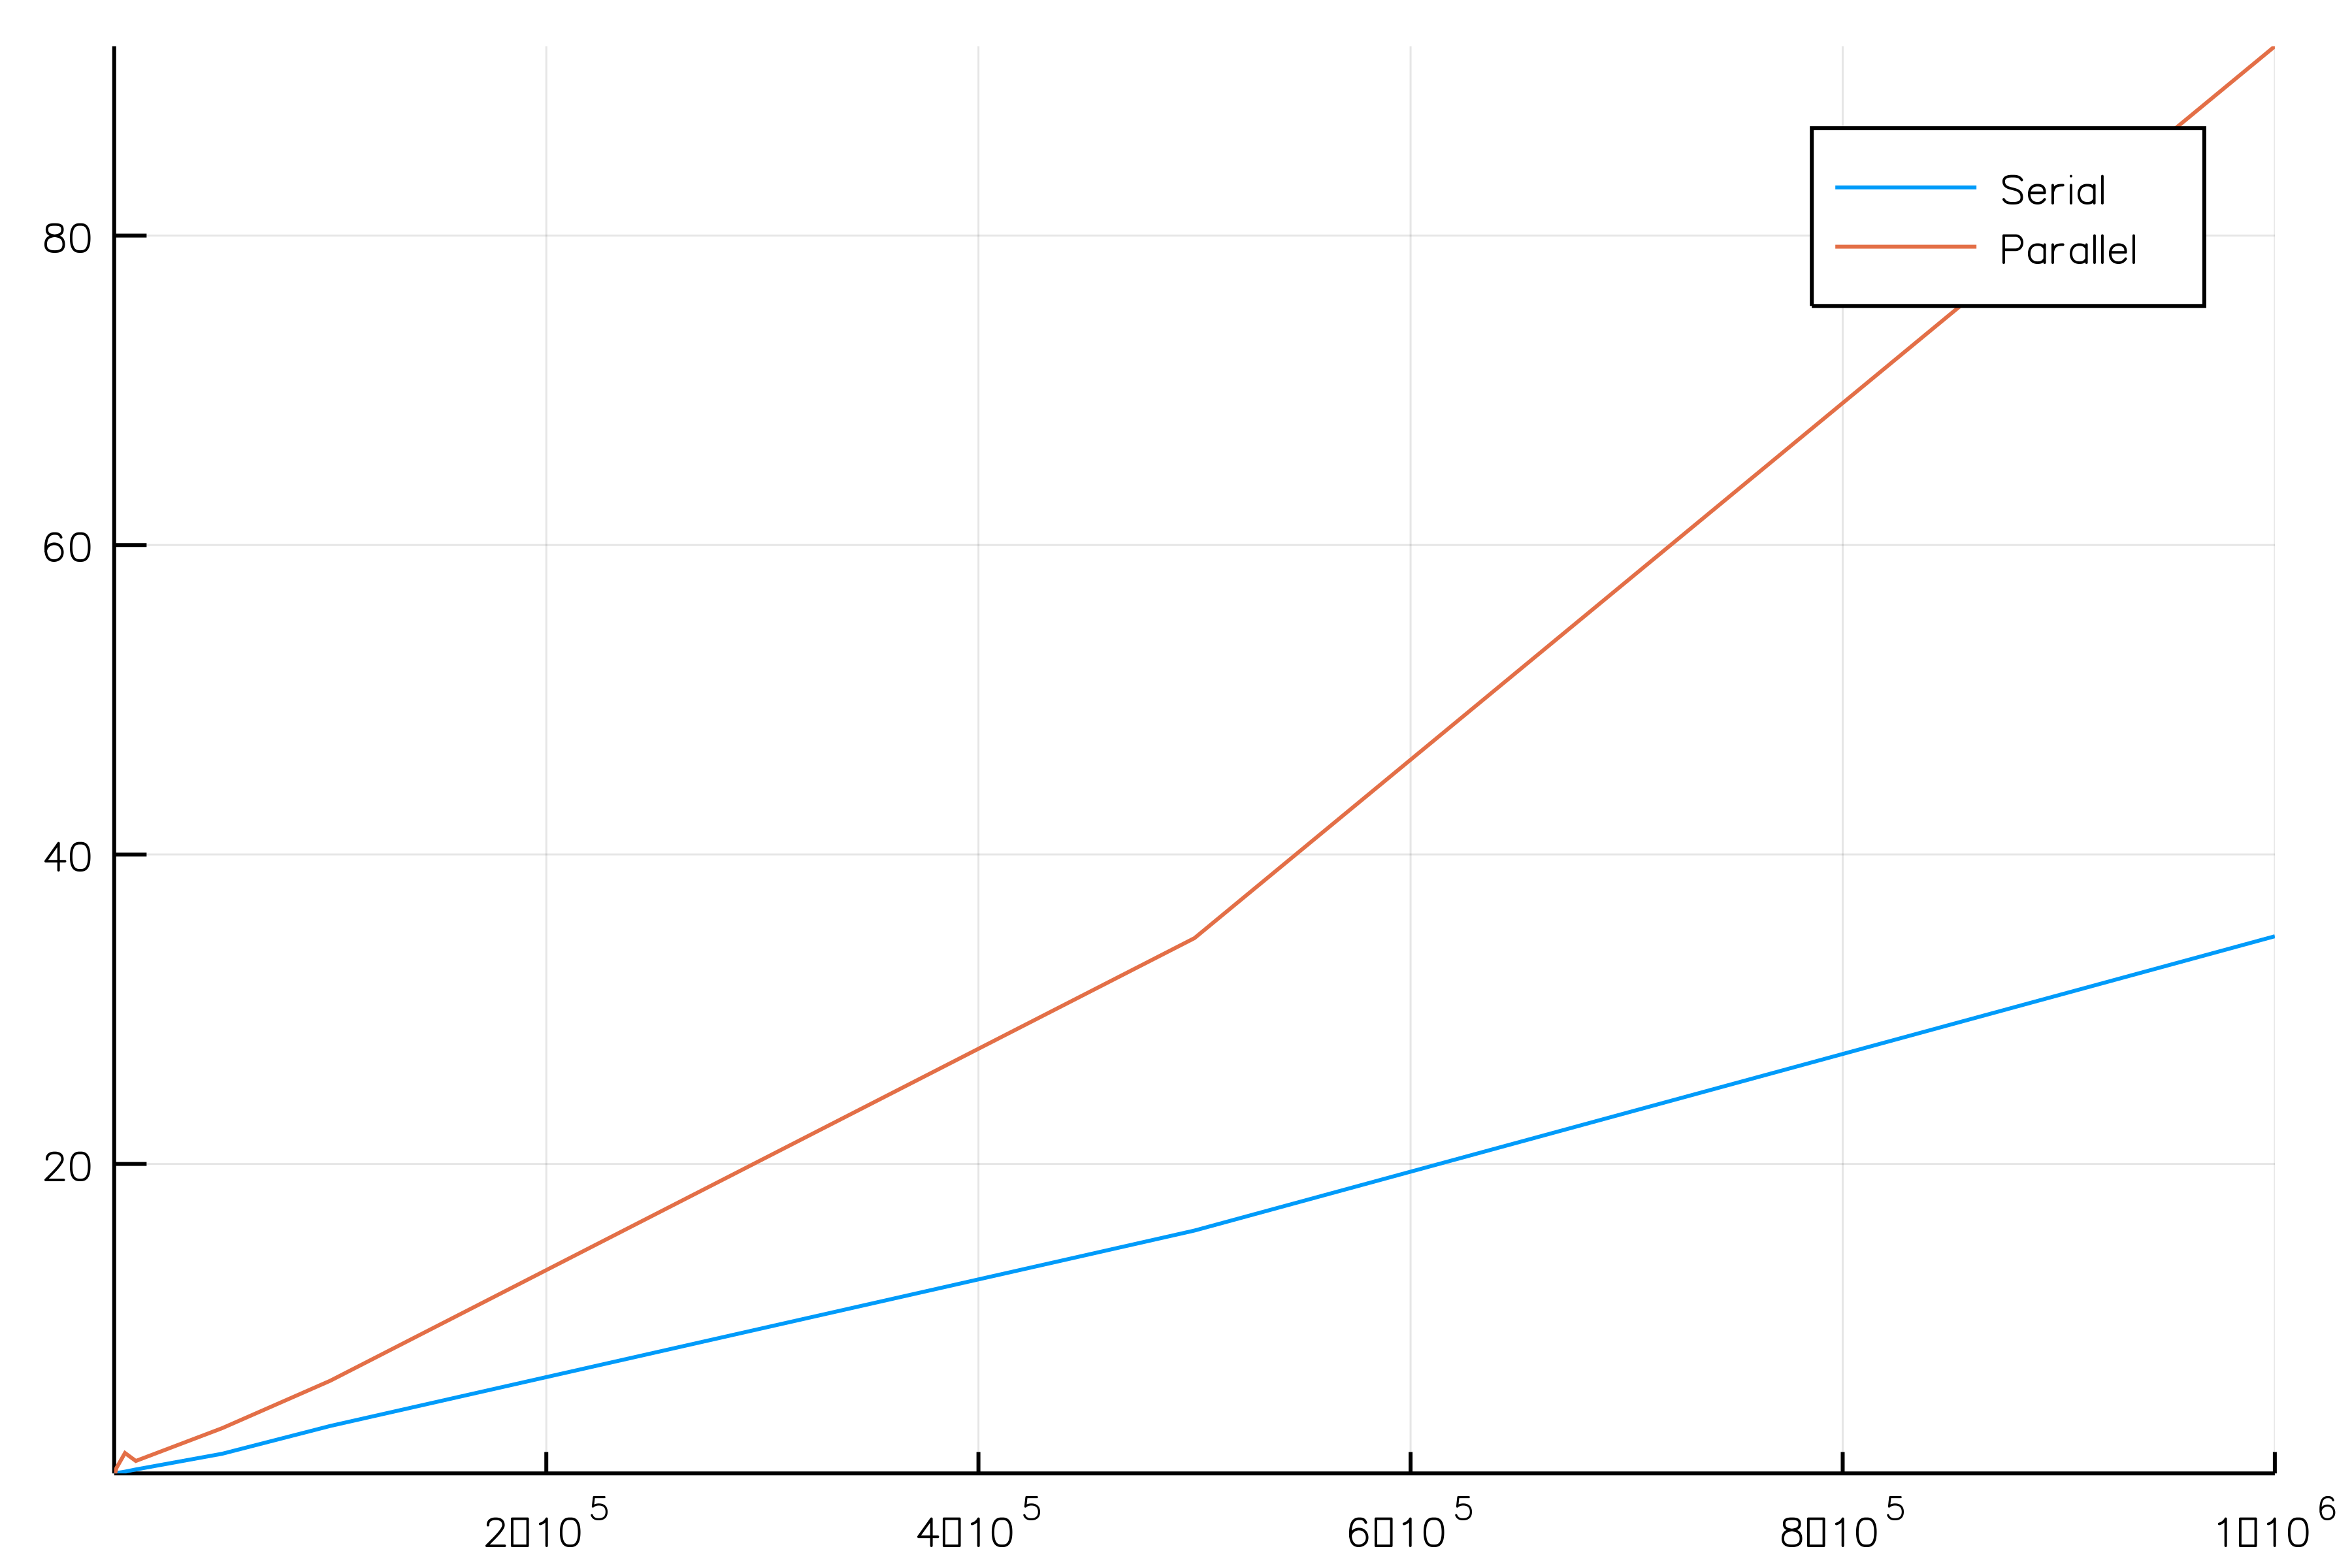
\includegraphics[scale=0.08]{compembedStruct.png}
\caption{Compared execution time of function embedtraversal on Tesla}
\end{figure}

%__________________________________________________________________________________________________________________________
\newpage

\subsection{removeDups}
\subsubsection{Conversion}
\framebox[5em][c]{\textbf{\normalsize Python}}
\begin{Verbatim}[fontsize=\footnotesize]
def removeDups (CW):
  CW = list(set(AA(tuple)(CW)))
  CWs = list(set(AA(tuple)(AA(sorted)(CW))))
  no_duplicates = defaultdict(list)
  for f in CWs: no_duplicates[f] = []
    for f in CW:
      no_duplicates[tuple(sorted(f))] += [f]
    CW = [f[0] for f in no_duplicates.values()]
  return CW
\end{Verbatim}
\framebox[5em][c]{\textbf{\normalsize Julia}}
\begin{Verbatim}[fontsize=\footnotesize]
function removeDups(CW)
  CW=collect(Set(CW))
  CWs=collect(map(sort,CW))
  no_duplicates=Dict()
  for f in CWs
    no_duplicates[f] = []
  end
  for f in CW
    no_duplicates[sort(f)]=[f]
  end
  CW=[f[1] for f in values(no_duplicates)]
  return CW
end 
\end{Verbatim}
\subsubsection{Parallelization}
\begin{Verbatim}[fontsize=\footnotesize]
function premoveDups(CW)
  CW=collect(Set(CW))
  CWs=collect(@sync pmap(sort,CW))
  no_duplicates=Dict()
  @parallel for f in CWs
    no_duplicates[f] = []
  end
  @parallel for f in CW
    no_duplicates[sort(f)]=[f]
  end
  @parallel for f in values(no_duplicates)
    append!(CW,f[1])
  end
  return CW
end
\end{Verbatim}
\subsubsection{Unit-Test}
\framebox[42em][c]{Serial Tests}
\begin{Verbatim}[fontsize=\footnotesize]
CW1=[[0,1,2,3],[4,5,6,7],[0,1,4,5],[2,3,6,7],[0,2,4,6],[1,3,5,7],[4,5,6,7],[8,9,10,11],
[4,5,8,9],[6,7,10,11],[4,6,8,10],[5,7,9,11]]
CW2=[[0,1,2,3],[4,5,6,7],[8,9,10,11],[12,13,14,15],[16,17,18,19]]

@testset "removeDups Tests" begin
  @testset "removeDups 3D" begin
    @test length(removeDups(CW1))<= length(CW1)
      @test typeof(removeDups(CW1))==Array{Array{Int64,1},1}
   end
   @testset "removeDups 2D" begin
      @test length(removeDups(CW2))<= length(CW2)
      @test typeof(removeDups(CW2))==Array{Array{Int64,1},1}
   end
end

\end{Verbatim}
\framebox[42em][c]{Palallel Tests}
\begin{Verbatim}[fontsize=\footnotesize]

CW1=[[0,1,2,3],[4,5,6,7],[0,1,4,5],[2,3,6,7],[0,2,4,6],[1,3,5,7],[4,5,6,7],[8,9,10,11],
[4,5,8,9],[6,7,10,11],[4,6,8,10],[5,7,9,11]]
CW2=[[0,1,2,3],[4,5,6,7],[8,9,10,11],[12,13,14,15],[16,17,18,19]]

@testset "premoveDups Tests" begin
   @testset "premoveDups 3D" begin
      @test length(premoveDups(CW1))<= length(CW1)
      @test typeof(premoveDups(CW1))==Array{Array{Int64,1},1}
   end
   @testset "premoveDups 2D" begin
      @test length(premoveDups(CW2))<= length(CW2)
      @test typeof(premoveDups(CW2))==Array{Array{Int64,1},1}
    end
end
\end{Verbatim}
\newpage
\subsection{struct2lar}
\subsubsection{Conversion}
\noindent \framebox[42em][c]{fixedPrec}
\begin{multicols}{2}
\noindent \framebox[5em][c]{\textbf{\normalsize Python}}
\begin{Verbatim}[fontsize=\scriptsize]
def fixedPrec(PRECISION):
  def fixedPrec0(value):
    out = round(value*10**(PRECISION))/10**(PRECISION)
    if out == -0.0: out = 0.0
      return str(out)
    return fixedPrec0 
\end{Verbatim}
\columnbreak
\framebox[5em][c]{\textbf{\normalsize Julia}}
\begin{Verbatim}[fontsize=\scriptsize]
function fixedPrec(PRECISION)
  function fixedPrec0(value) 
    out=round.(value,PRECISION)
    if out==-0.0
      out=0.0
    end
    return string(out)
  end
  return fixedPrec0
end
\end{Verbatim}
\end{multicols}

\noindent \framebox[42em][c]{vcode}
\begin{multicols}{2}
\noindent \framebox[5em][c]{\textbf{\normalsize Python}}
\begin{Verbatim}[fontsize=\scriptsize]
def vcode (PRECISION=4):
  def vcode0 (vect):
    return prepKey(AA(fixedPrec(PRECISION))(vect))
  return vcode0  
\end{Verbatim}
\columnbreak
\framebox[5em][c]{\textbf{\normalsize Julia}}
\begin{Verbatim}[fontsize=\scriptsize]
function vcode(PRECISION=4)
  function vcode0(vect)
    return fixedPrec(PRECISION)(vect)
  end
  return vcode0
end
\end{Verbatim}
\end{multicols}
\noindent \framebox[5em][c]{\textbf{\normalsize Python}}
\begin{Verbatim}[fontsize=\footnotesize]
def struct2lar(structure,metric=ID):
  listOfModels = evalStruct(structure)
  vertDict = dict()
  index,defaultValue,CW,W,FW = -1,-1,[],[],[]
  for model in listOfModels:
    if isinstance(model,Model):
      V= model.verts
      FV=model.cells
    elif (isinstance(model,tuple) or isinstance(model,list)):
      if len(model)==2:
	V,FV=model
	dim=len(model)
      elif len(model)==3: 
	V,FV,EV,dim=model,len(model)
	for k,incell in enumerate(EV):
	  outcell = []
	  for v in incell:
	    key = vcode(4)(V[v])
	    if vertDict.get(key,defaultValue) == defaultValue:
	      index += 1
	      vertDict[key] = index
	      outcell += [index]
	      W += [eval(key)]
	    else: 
	      outcell += [vertDict[key]]
	  FW += [outcell]
    for k,incell in enumerate(FV):
      outcell = []
      for v in incell:
	key = vcode(4)(V[v])
	if vertDict.get(key,defaultValue) == defaultValue:
	  index += 1
	  vertDict[key] = index
	  outcell += [index]
	  W += [eval(key)]
	else: 
	  outcell += [vertDict[key]]
      CW += [outcell]
  if ((isinstance(model,tuple) or isinstance(model,list))and len(model)==2) or 
  ((isinstance(model,Model)and model.n==2)):
    if len(CW[0])==2:
      CW = list(set(AA(tuple)(AA(sorted)(CW))))
    else: CW = removeDups(CW)
    return metric(W),CW
  if ((isinstance(model,tuple) or isinstance(model,list))and len(model)==3):
    FW = list(set(AA(tuple)(AA(sorted)(FW))))
    CW = removeDups(CW)
    return metric(W),CW,FW
\end{Verbatim}
\noindent \framebox[5em][c]{\textbf{\normalsize Julia}}
\begin{Verbatim}[fontsize=\footnotesize]
function struct2lar(structure)
  listOfModels=evalStruct(structure)
  vertDict= Dict()
  index,defaultValue,CW,W,FW = -1,-1,[],[],[]
  for model in listOfModels
    if  length(model)==2
      V,FV=model
    elseif lenght(model)==3
      V,FV,EV=model
    end
    for (k,incell) in enumerate(FV)
      outcell=[ ]
      for v in incell
	key=vcode(4)(V[v+1])
	if get(vertDict,key,defaultValue)==defaultValue
	  index =index+1
	  vertDict[key]=index
	  append!(outcell,index)
	  append!(W,[eval(parse(key))])
	else
	  append!(outcell,vertDict[key])
	end
      end
      append!(CW,[outcell])
    end
    if length(model)==3
      for (k,incell) in enumerate(FV)
	outcell=[]
	for v in incell
	  key=vcode(4)(V[v+1])
	  if get(vertDict,key,defaultValue)==defaultValue
	    index =index+1
	    vertDict[key]=index
	    append!(outcell,[index])
	    append!(W,[eval(parse(key))])
	  else
	    append!(outcell,vertDict[key])
	  end
	end
	append!(FW,[outcell])
      end
    end
  end
  if length(listOfModels[end])==2
    if length(CW[1])==2
      CW=map(Tuple,map(sort,CW))
    else
      CW=removeDups(CW)
    end
    return W,CW
  end
  if length(listOfModels[end])==3
    FW=map(Tuple,map(sort,FW))
    CW=removeDups(CW)
    return W,CW,FW
    end
end

\end{Verbatim}
\subsubsection{Parallelization}
\begin{Verbatim}[fontsize=\footnotesize]

@everywhere function pstruct2lar(structure)
  listOfModels=pevalStruct(structure)
  vertDict= Dict()
  index,defaultValue,CW,W,FW = -1,-1,[],[],[]
  for model in listOfModels
    if  length(model)==2
      V,FV=model
    elseif lenght(model)==3
      V,FV,EV=model
    end
    @sync begin
      for (k,incell) in enumerate(FV)
	outcell=[]
	@async begin
	  for v in incell
	    key=vcode(4)(V[v+1])
	    if get(vertDict,key,defaultValue)==defaultValue
	      index =index+1
	      vertDict[key]=index
	      append!(outcell,index)
	      append!(W,[eval(parse(key))])
	    else
	      append!(outcell,vertDict[key])
	    end
	  end
	end
	append!(CW,[outcell])
      end
    end
    if length(model)==3
      @sync begin
	for (k,incell) in enumerate(FV)
	  outcell=[]
	  @async begin
	    for v in incell
	      key=vcode(4)(V[v+1])
	      if get(vertDict,key,defaultValue)==defaultValue
		index =index+1
		vertDict[key]=index
		append!(outcell,[index])
		append!(W,[eval(parse(key))])
	      else
		append!(outcell,vertDict[key])
	      end
	    end
	  end
	  append!(FW,[outcell])
	end
      end
    end
  end
  if length(listOfModels[end])==2
    if length(CW[1])==2
      CW=pmap(Tuple,pmap(sort,CW))
    else
      CW=premoveDups(CW)
    end
    return W,CW
  end
  if length(listOfModels[end])==3
    FW=pmap(Tuple,pmap(sort,FW)) 
    CW=premoveDups(CW)
    return W,CW,FW
  end
end

\end{Verbatim}

\subsubsection{Unit-Test}
\framebox[42em][c]{Serial Tests}
\begin{Verbatim}[fontsize=\footnotesize]

@testset "struct2lar Tests" begin
  @testset "struct2lar 2D" begin
    square=([[0, 0],[0,1],[1,0],[1,1]],[[0,1,2,3]])
    table=larApply(t(-0.5,-0.5))(square)
    structure=Struct([repeat([table,r(pi/2)],outer=2)...])
    @test typeof(struct2lar(structure))==Tuple{Array{Any,1},Array{Array{Any,1},1}}
    @test length(struct2lar(structure)[1][1])==2
  end
  
  @testset "struct2lar 3D" begin
    BV=[[0,1,2,3],[4,5,6,7],[0,1,4,5],[2,3,6,7],[0,2,4,6],[1,3,5,7]]
    V=[[0,0,0],[0,0,1],[0,1,0],[0,1,1],[1,0,0],[1,0,1],[1,1,0],[1,1,1]]
    block=[V,BV]
    structure=Struct(repeat([block,t(1,0,0)],outer=2));
    @test typeof(struct2lar(structure))==Tuple{Array{Any,1},Array{Array{Any,1},1}}
    @test length(struct2lar(structure)[1][1])==3
  end
end

\end{Verbatim}

\noindent\framebox[42em][c]{Palallel Tests}
\begin{Verbatim}[fontsize=\footnotesize]

@testset "pstruct2lar Tests" begin
  @testset "pstruct2lar 2D" begin
    square=([[0,0],[0,1],[1,0],[1,1]],[[0,1,2,3]])
    table=plarApply(t(-0.5,-0.5))(square)
    structure=pStruct([repeat([table,r(pi/2)],outer=2)...])
    @test typeof(pstruct2lar(structure))==Tuple{Array{Any,1},Array{Any,1}}
    @test length(pstruct2lar(structure)[1][1])==2
  end
  
  @testset "pstruct2lar 3D" begin
    BV=[[0,1,2,3],[4,5,6,7],[0,1,4,5],[2,3,6,7],[0,2,4,6],[1,3,5,7]]
    V=[[0,0,0],[0,0,1],[0,1,0],[0,1,1],[1,0,0],[1,0,1],[1,1,0],[1,1,1]]
    block=[V,BV]
    structure=pStruct(repeat([block,t(1,0,0)],outer=2));
    @test typeof(pstruct2lar(structure))==Tuple{Array{Any,1},Array{Any,1}}
    @test length(pstruct2lar(structure)[1][1])==3
   end
end

\end{Verbatim}

\subsubsection{Results}
\textbf{Execution time on PC}
\begin{Verbatim}[fontsize=\footnotesize]
times=[]
ptimes=[]
input=[]

for i in range(1,length(l)-1)
  push!(input,Struct([repeat([l[i]],outer=i)...]))
end
append!(times,Time(struct2lar,[input[i]]) for i in range(1,length(input)))
append!(ptimes,Time(pstruct2lar,[input[i]]) for i in range(1,length(input)))


plot(times,xlabel="input",xlims=(0,length(times)+2),ylabel="time(s)",label=["Serial"])
plot(ptimes,xlabel="input",xlims=(0,length(times)+2),ylabel="time(s)",label=["Parallel"])

\end{Verbatim}

\begin{figure*}[!h]
\centering
\subfloat[Serial]{%
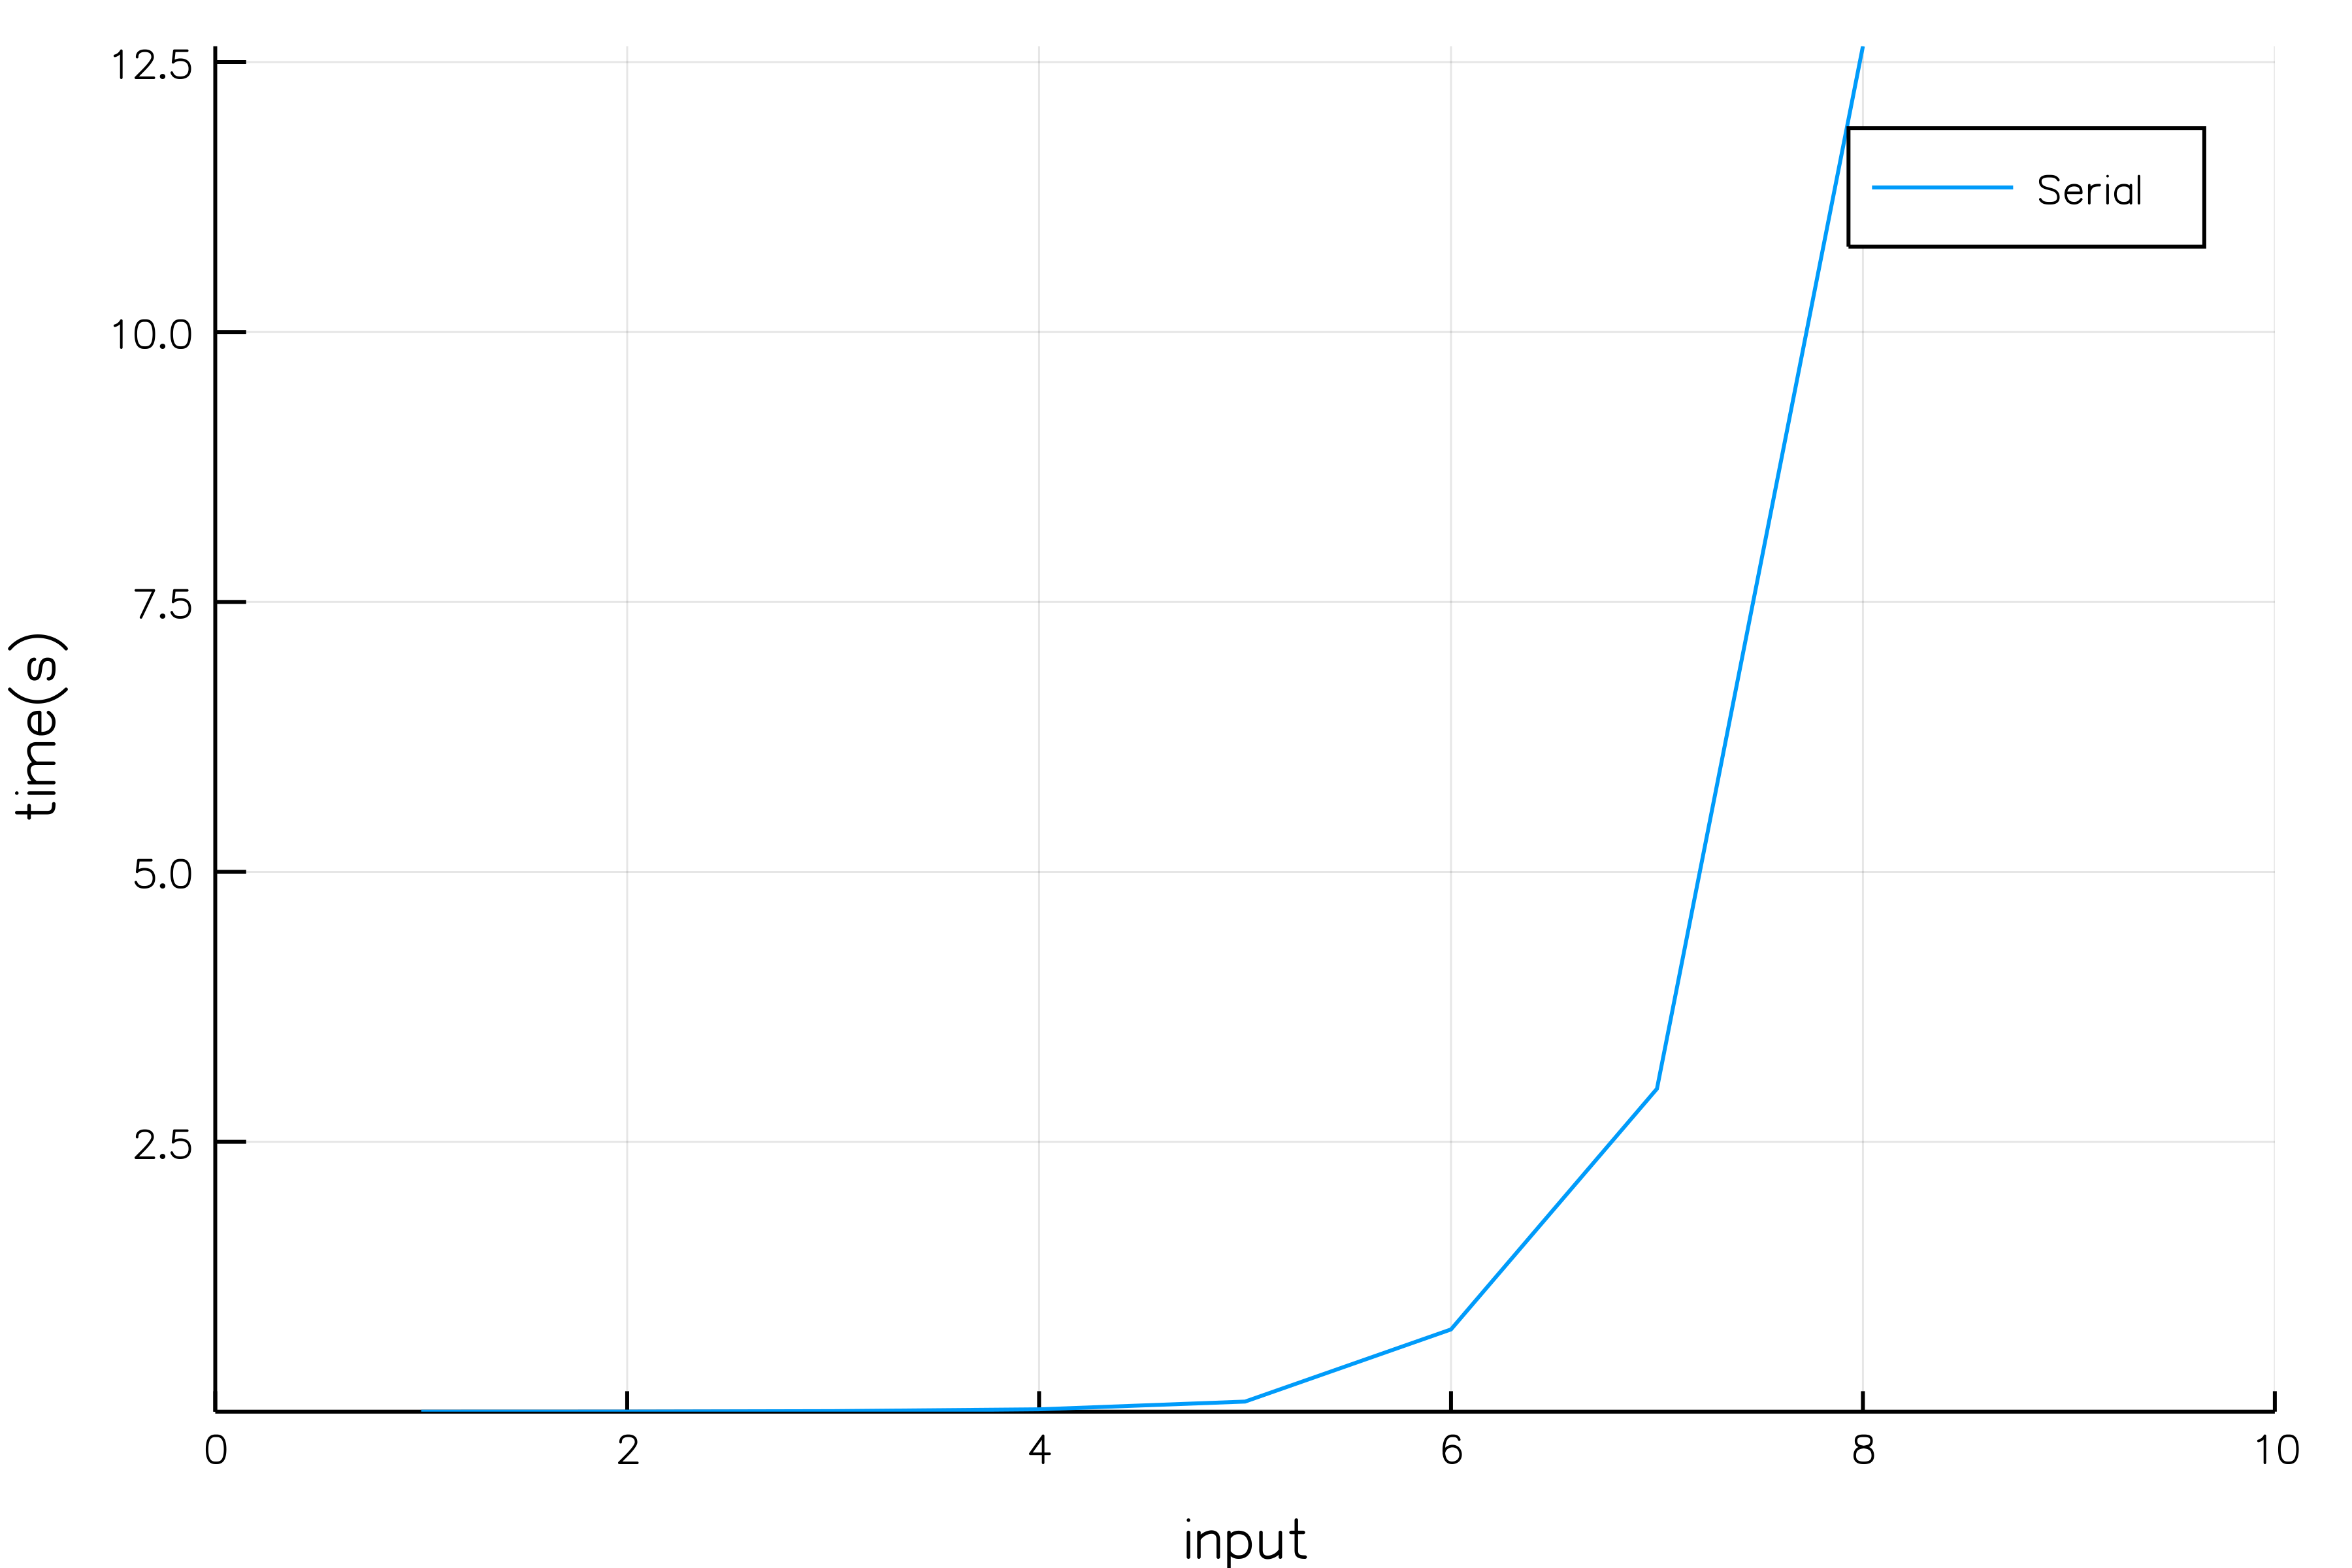
\includegraphics[scale=0.060]{struct2larSerial.png}
}
\subfloat[Parallel]{%
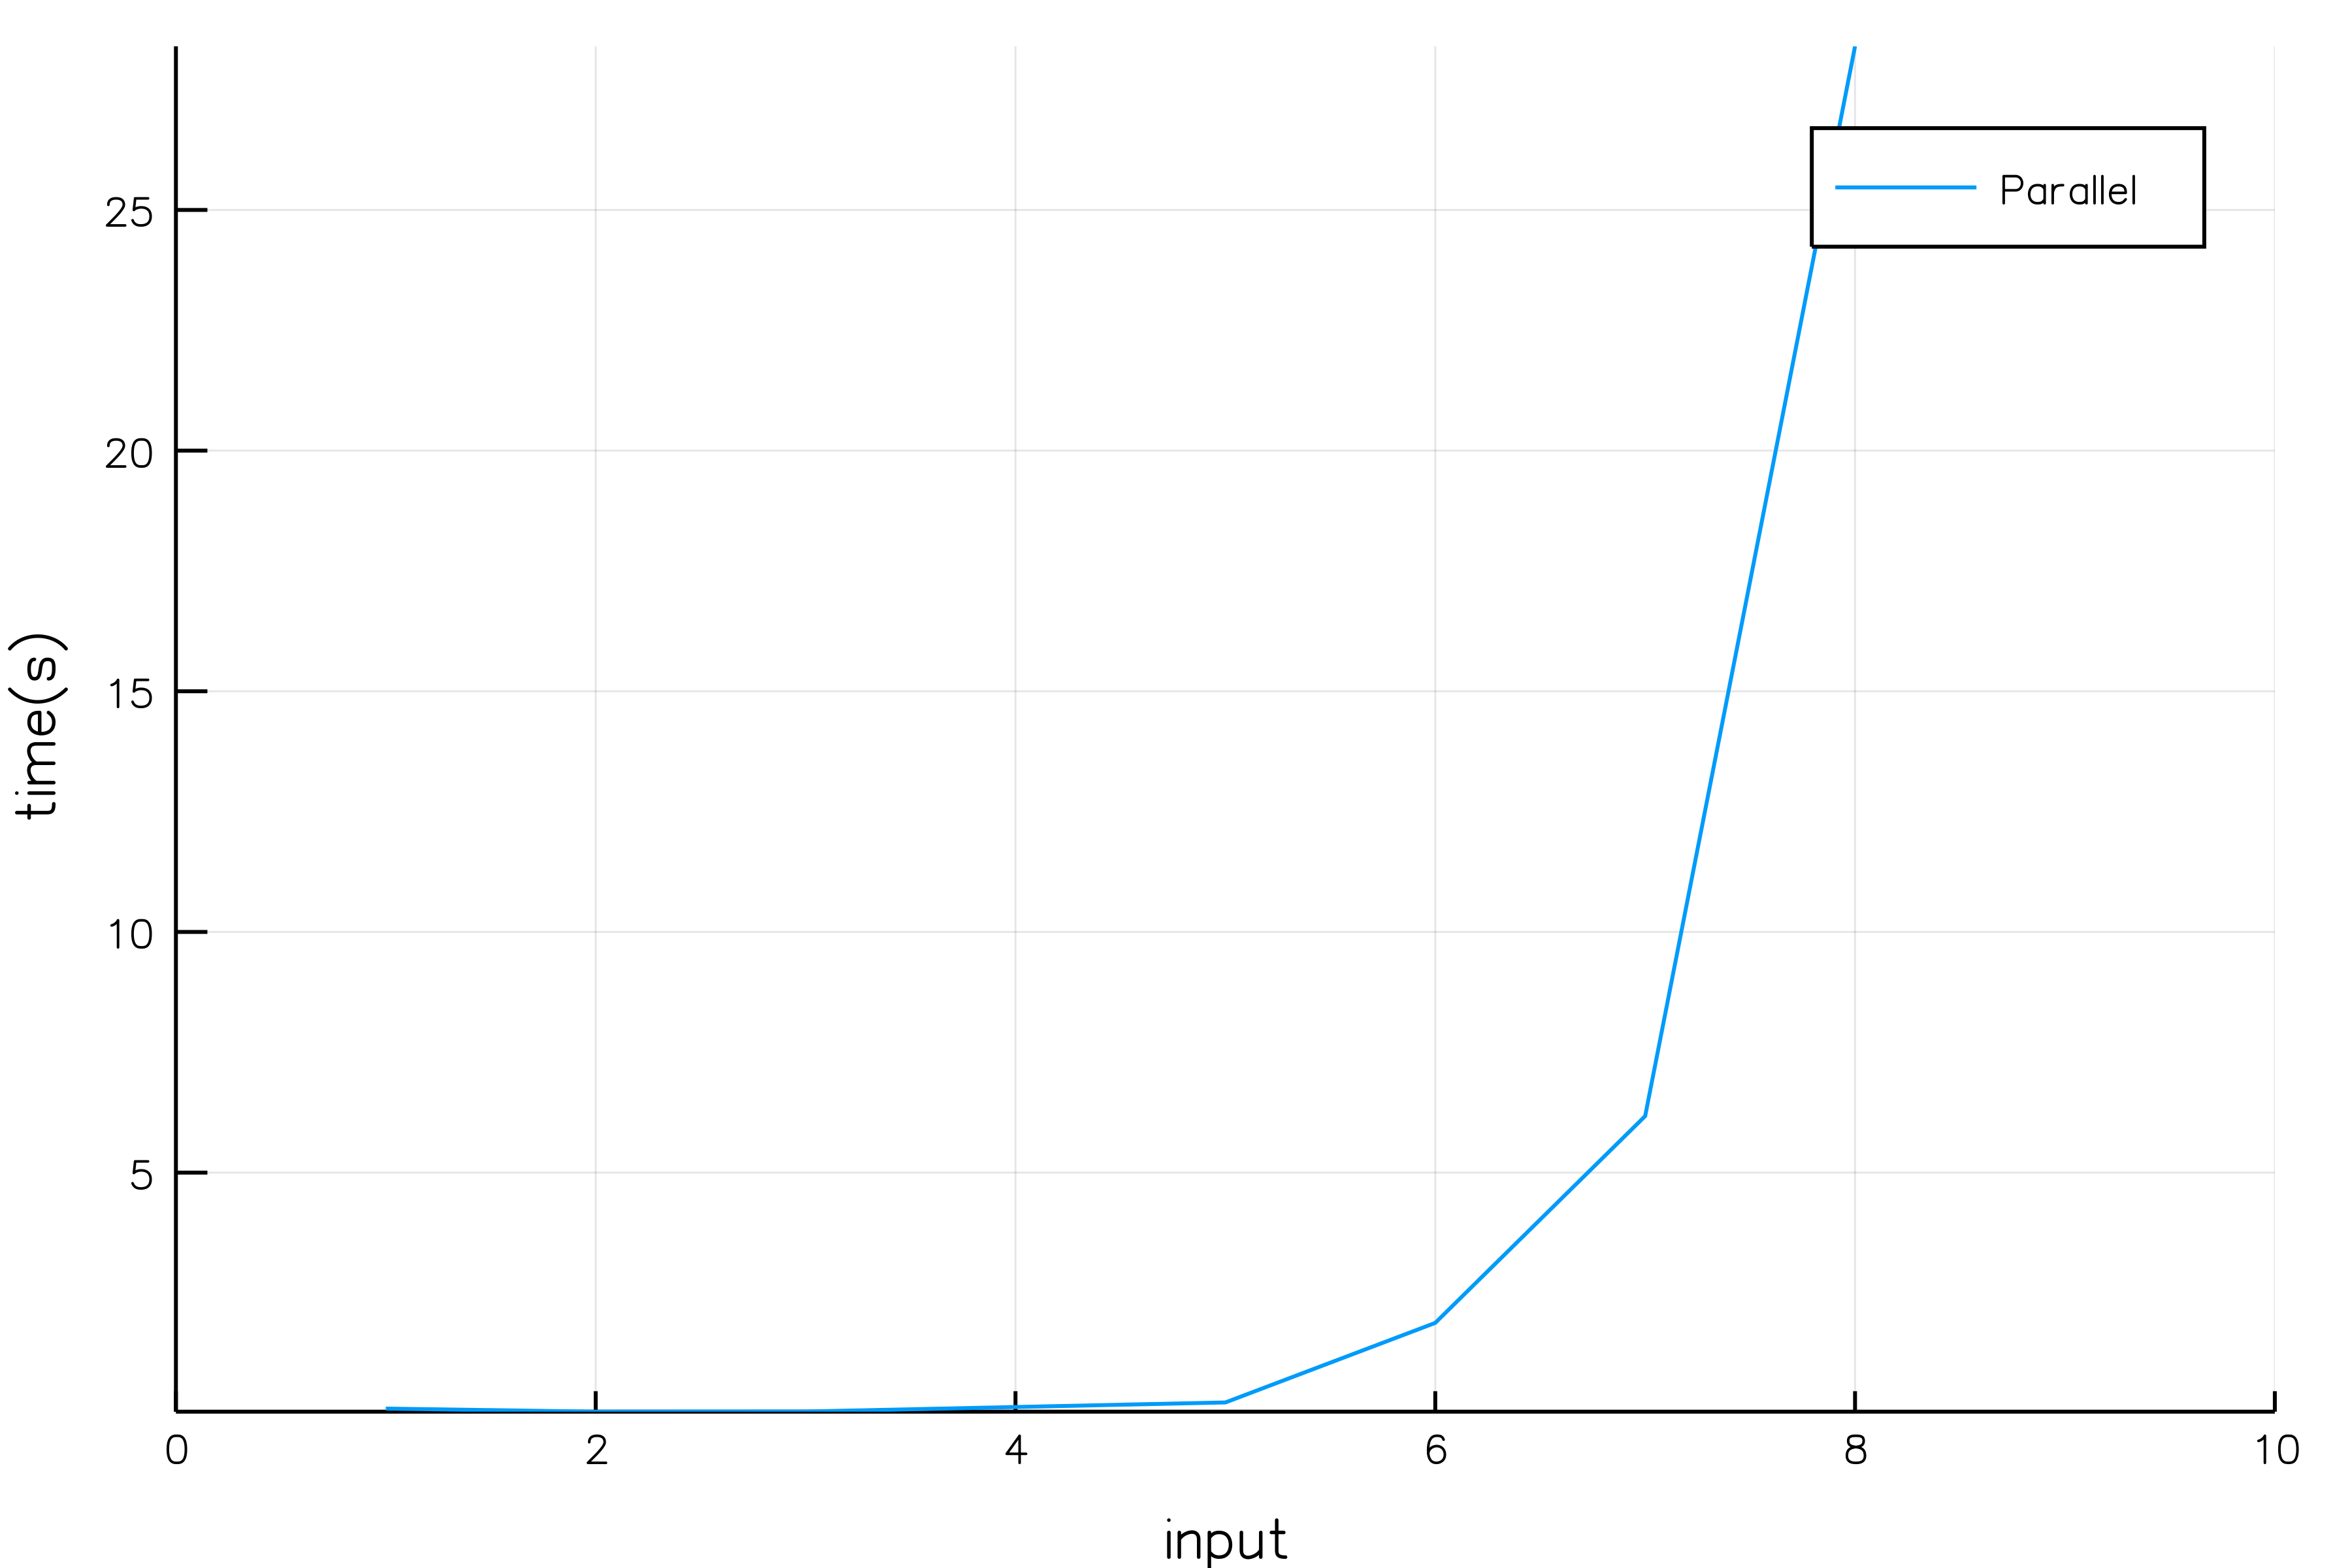
\includegraphics[scale=0.060]{struct2larParallel.png}
}
\caption{Execution time of function struct2lar}
\end{figure*}
%__________________________________________________________________________________________________________________________
\newpage

\noindent\framebox[42em][c]{Compare}
\begin{Verbatim}[fontsize=\footnotesize]

plot([times,ptimes],xlabel="input",xlims=(0,length(times)+2),ylabel="time(s)",
label=["Serial","Parallel"])

\end{Verbatim}
\vspace{20px}

\begin{figure}[!h]
\centering
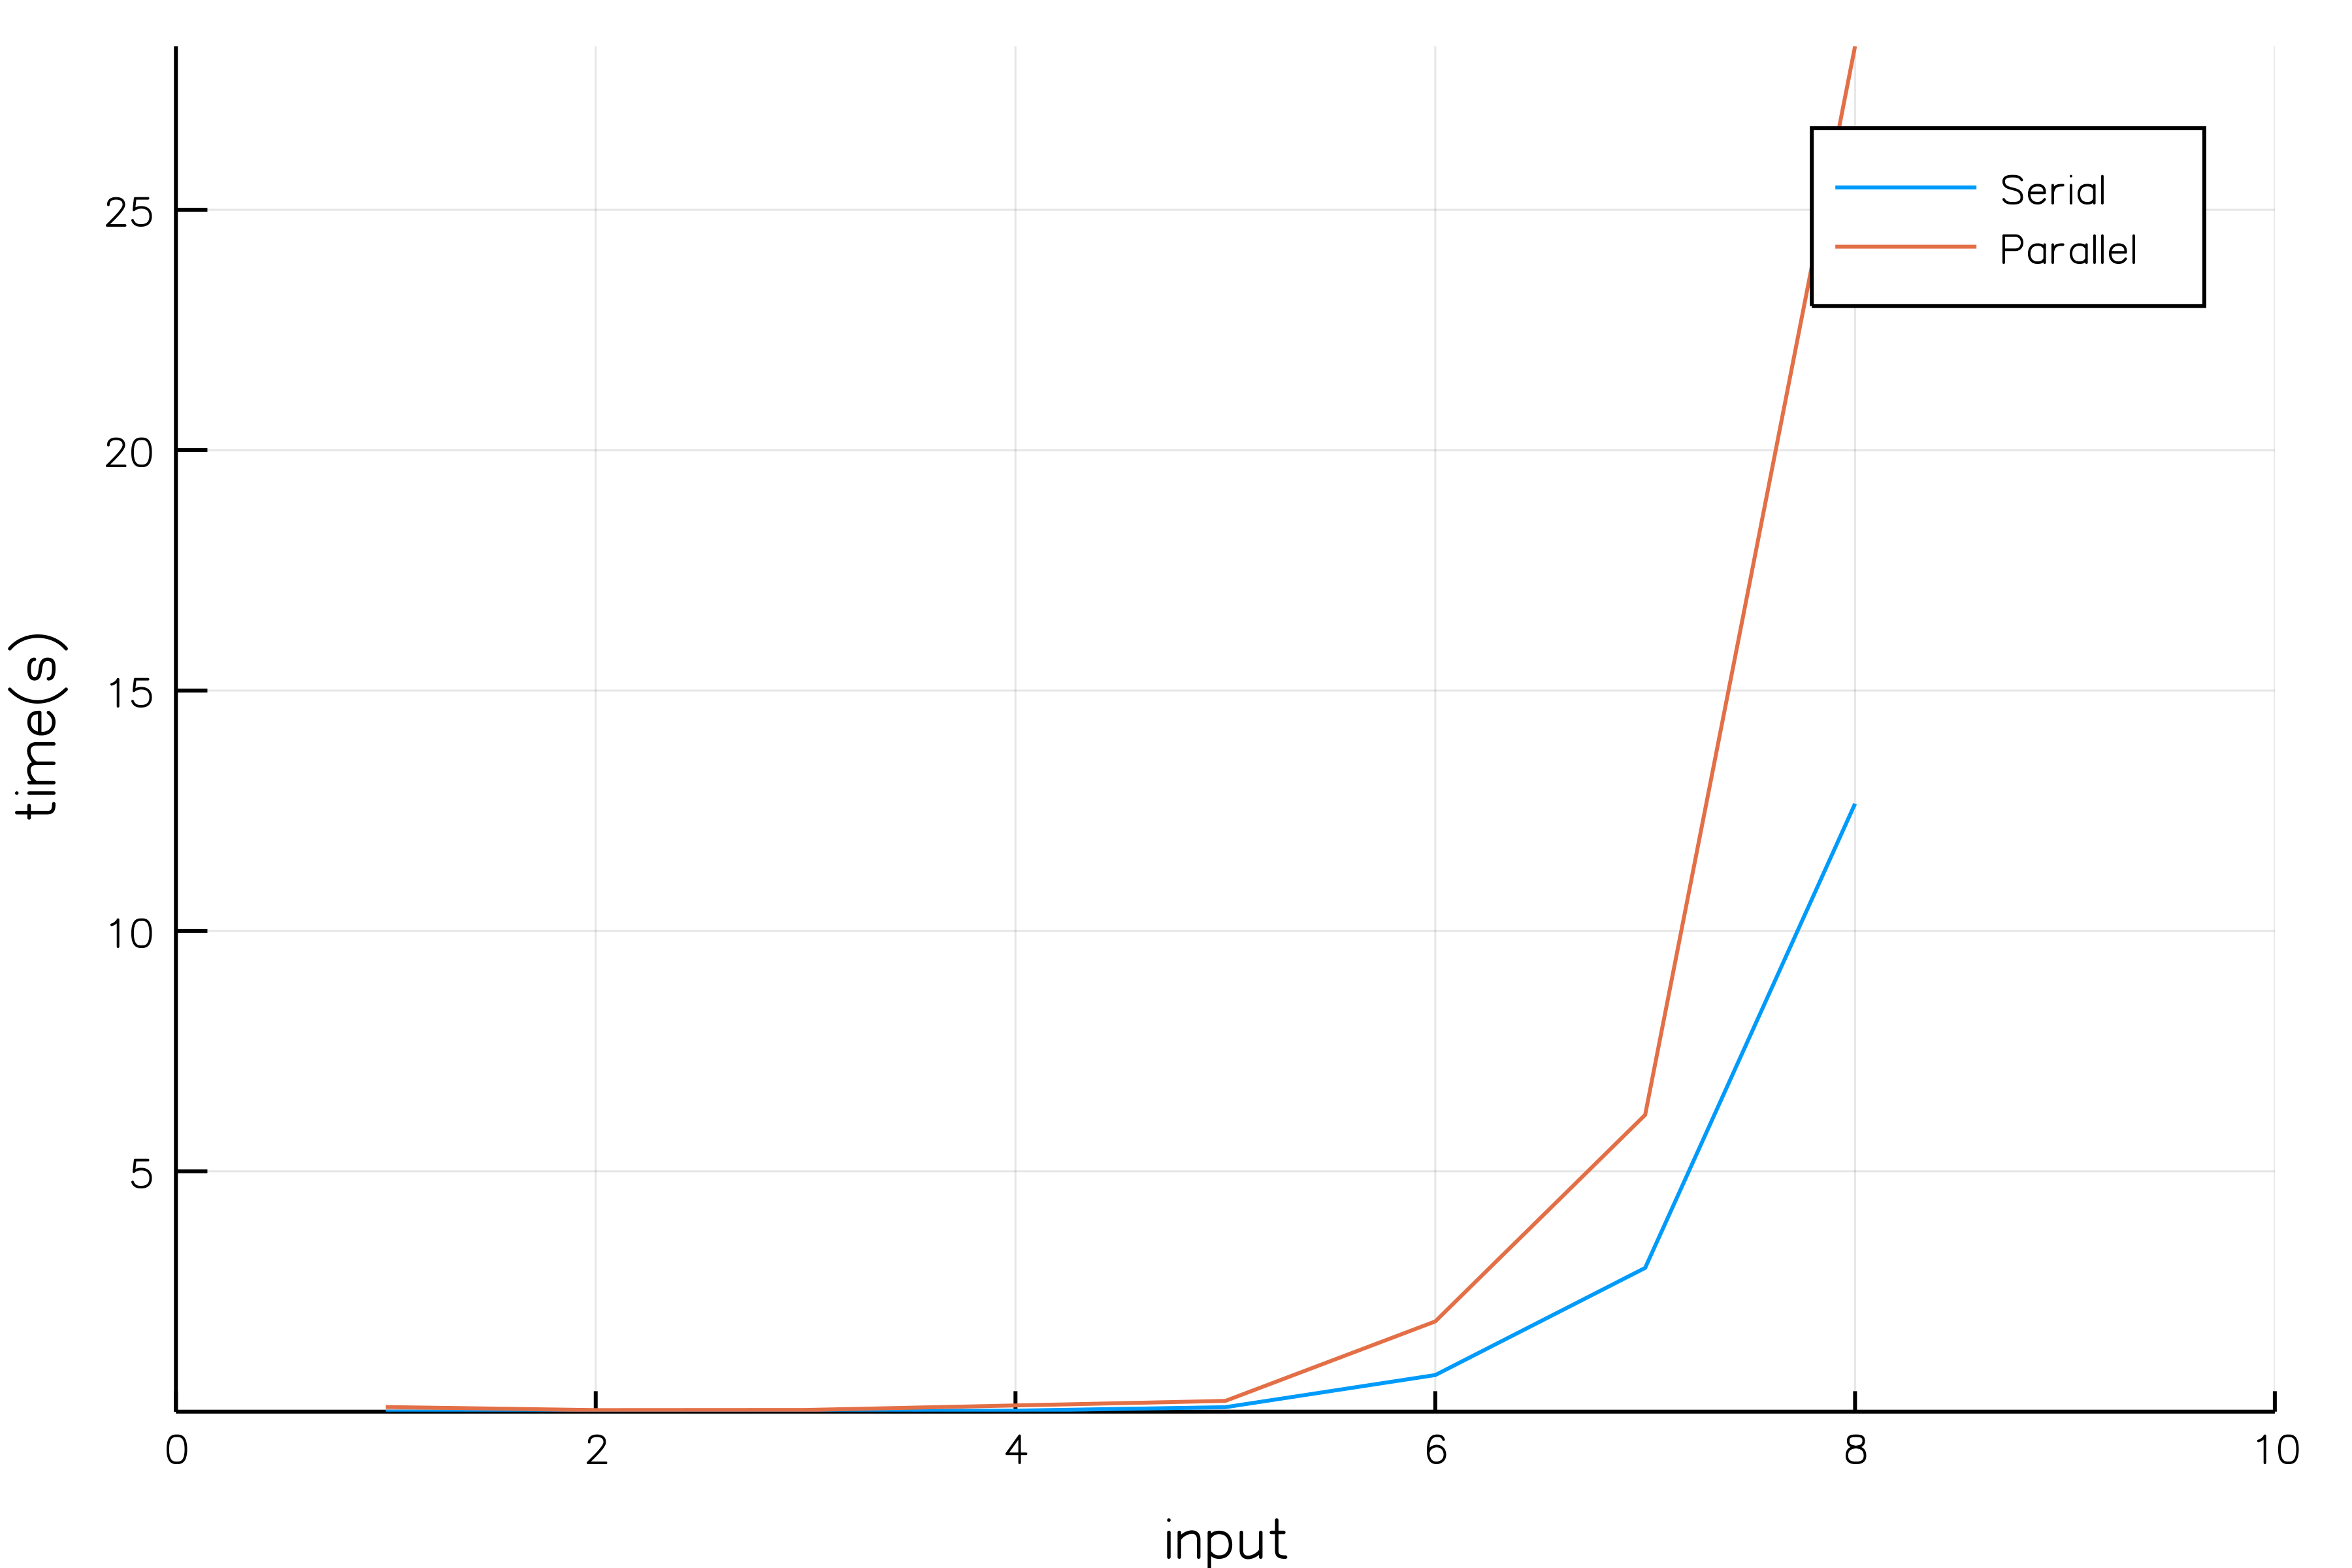
\includegraphics[scale=0.08]{struct2larC.png}
\caption{Compared execution time of function struct2lar}
\end{figure}
\vspace{20px}

\noindent\textbf{Execution time on Tesla}
\begin{Verbatim}[fontsize=\footnotesize]

input=[1,10,20,50,10^2,2*10^2,5*10^2,10^3,2*10^3]
y,yp=timeFstruct(struct2lar,pstruct2lar,square,input)

\end{Verbatim}

%__________________________________________________________________________________________________________________________
\newpage

\begin{Verbatim}[fontsize=\footnotesize]
p=plot(input,y,xaxis="input",yaxis="time",xlims=(0,length(input)+1),
     ylims=(0,maximum(y)+0.5), label=["Serial"],lw=2)
pp=plot(input,yp,xaxis="input",yaxis="time",xlims=(0,length(input)+1),
       ylims=(0,maximum(y)+0.5),label=["Parallel"],lw=2)
\end{Verbatim}

\begin{figure*}[!h]
\centering
\subfloat[Serial]{%
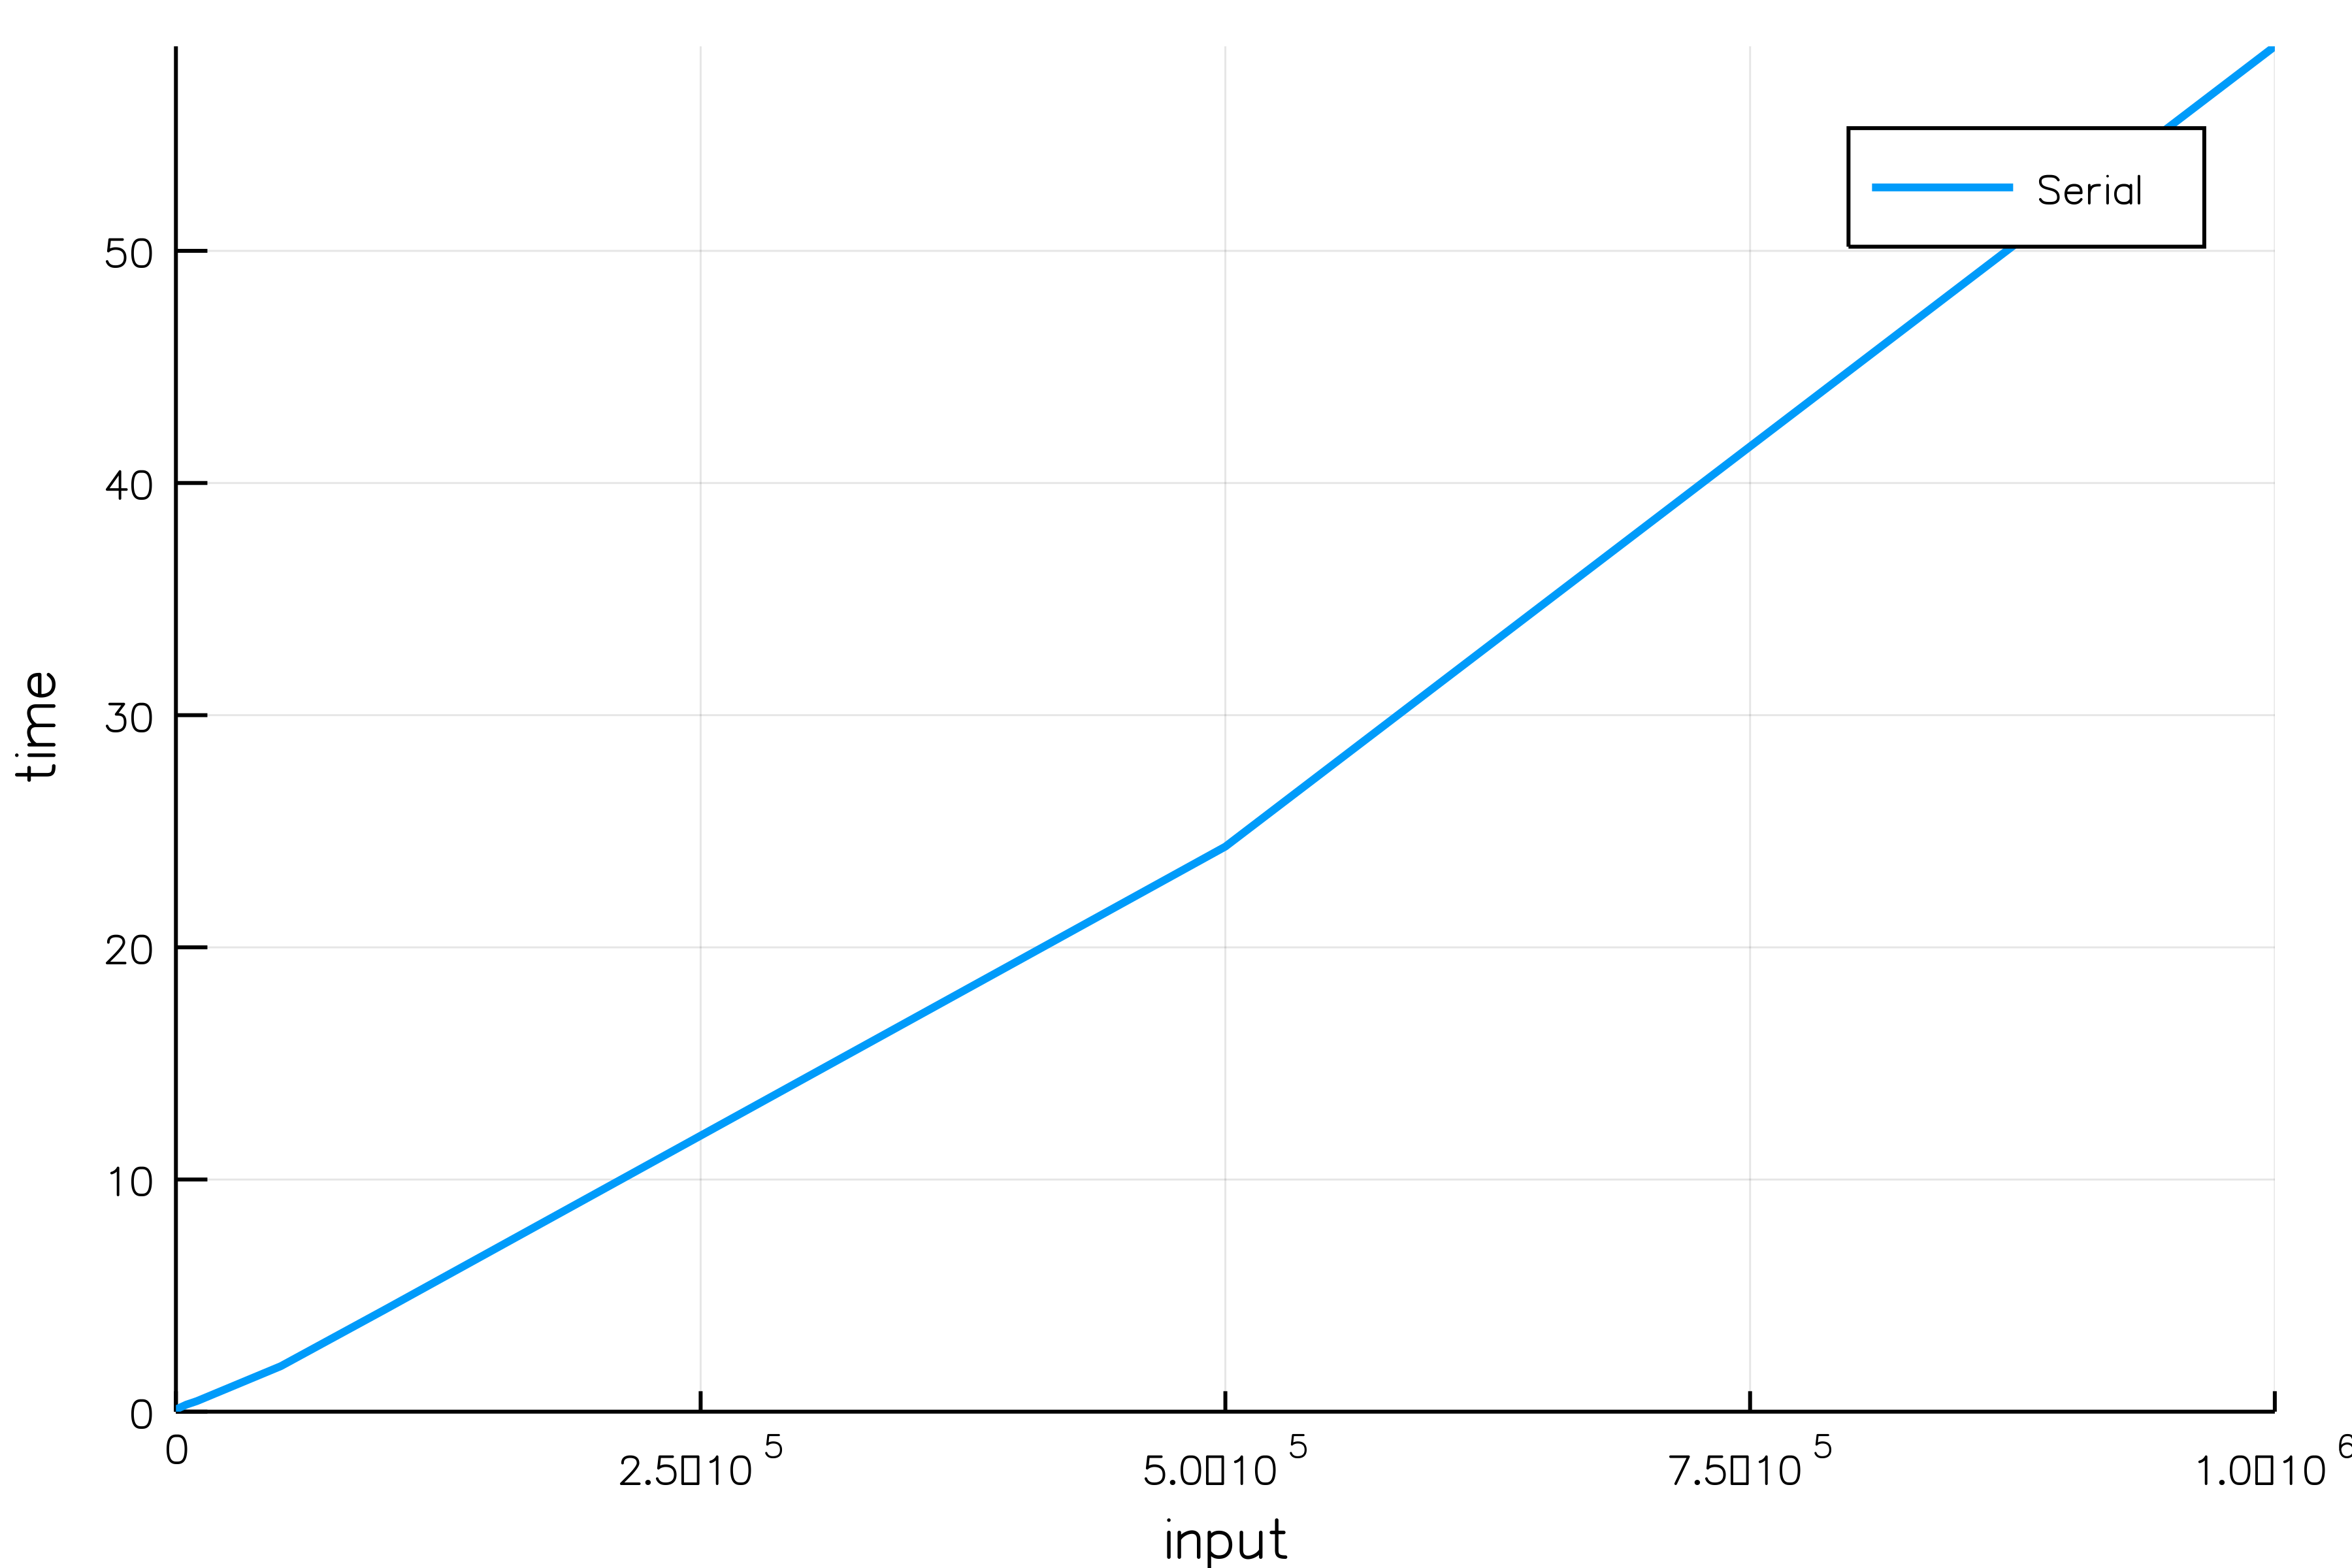
\includegraphics[scale=0.060]{struct2lar.png}
}
\subfloat[Parallel]{%
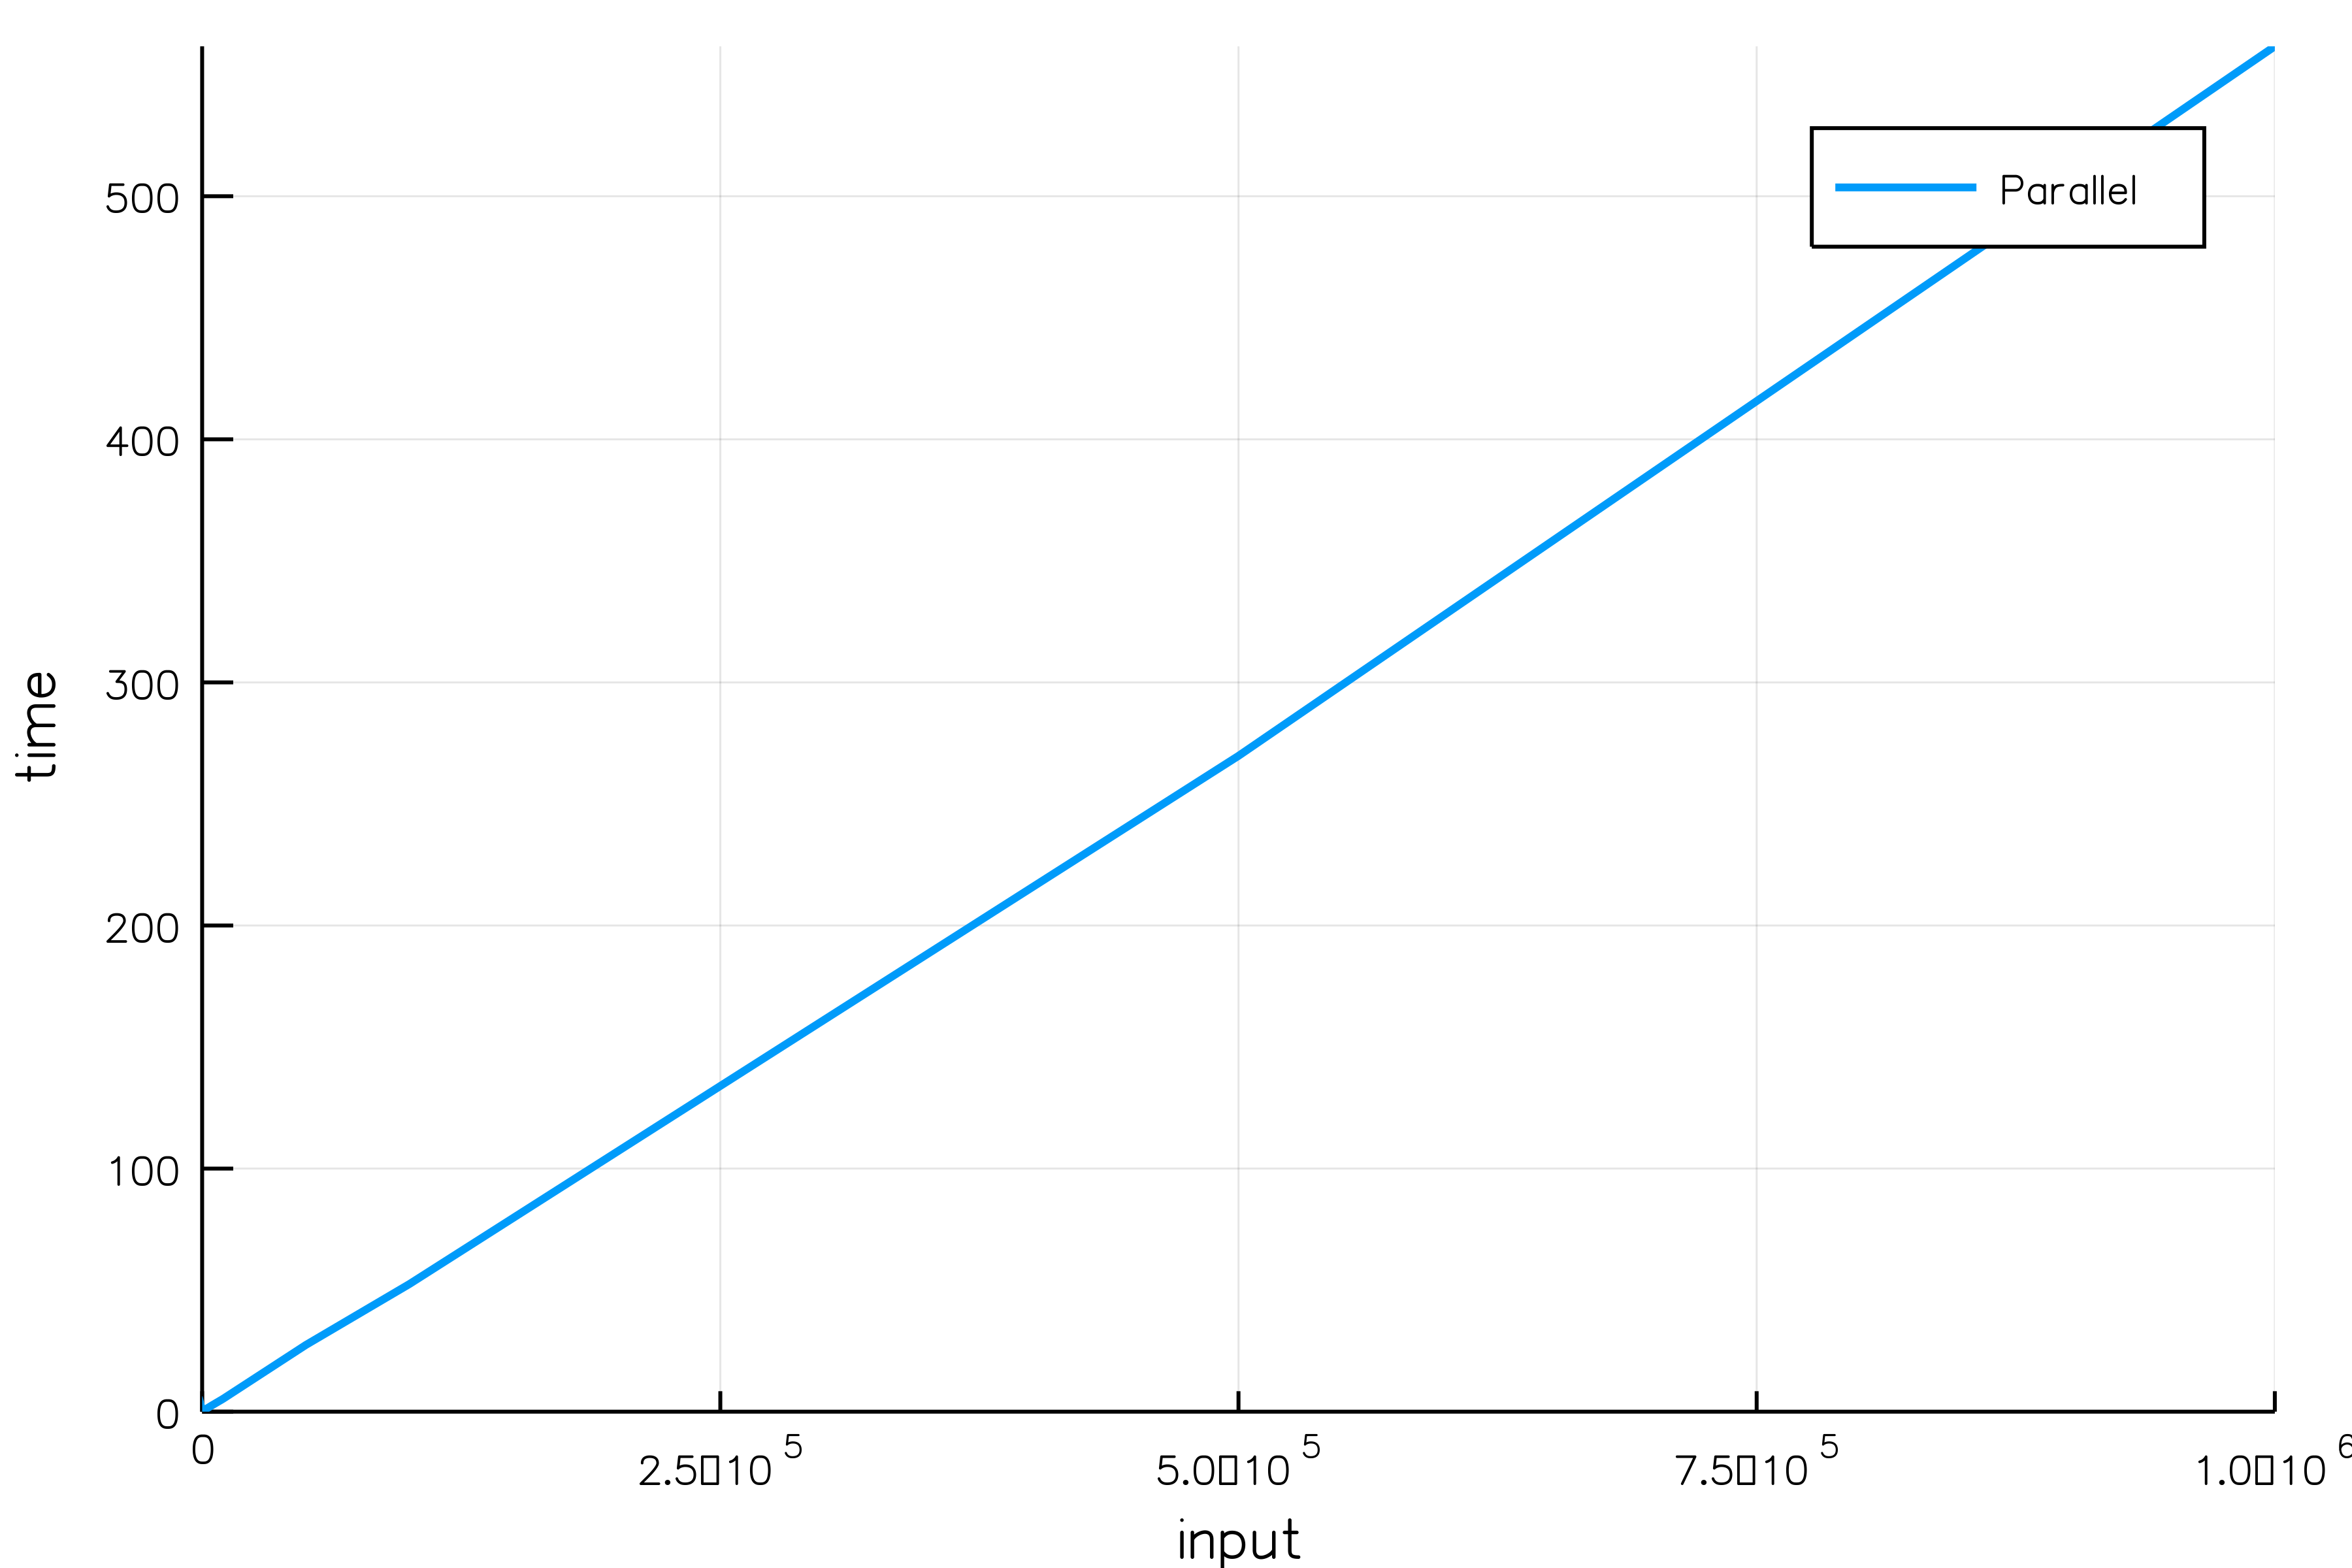
\includegraphics[scale=0.060]{pstruct2lar.png}
}
\caption{Execution Time of function struct2lar on Tesla}
\end{figure*}


\noindent\framebox[42em][c]{Compare}
\begin{Verbatim}[fontsize=\footnotesize]
yc=[y,yp]
pc=plot(input,yc,label=["Serial" "Parallel"])
\end{Verbatim}

\begin{figure}[!h]
\centering
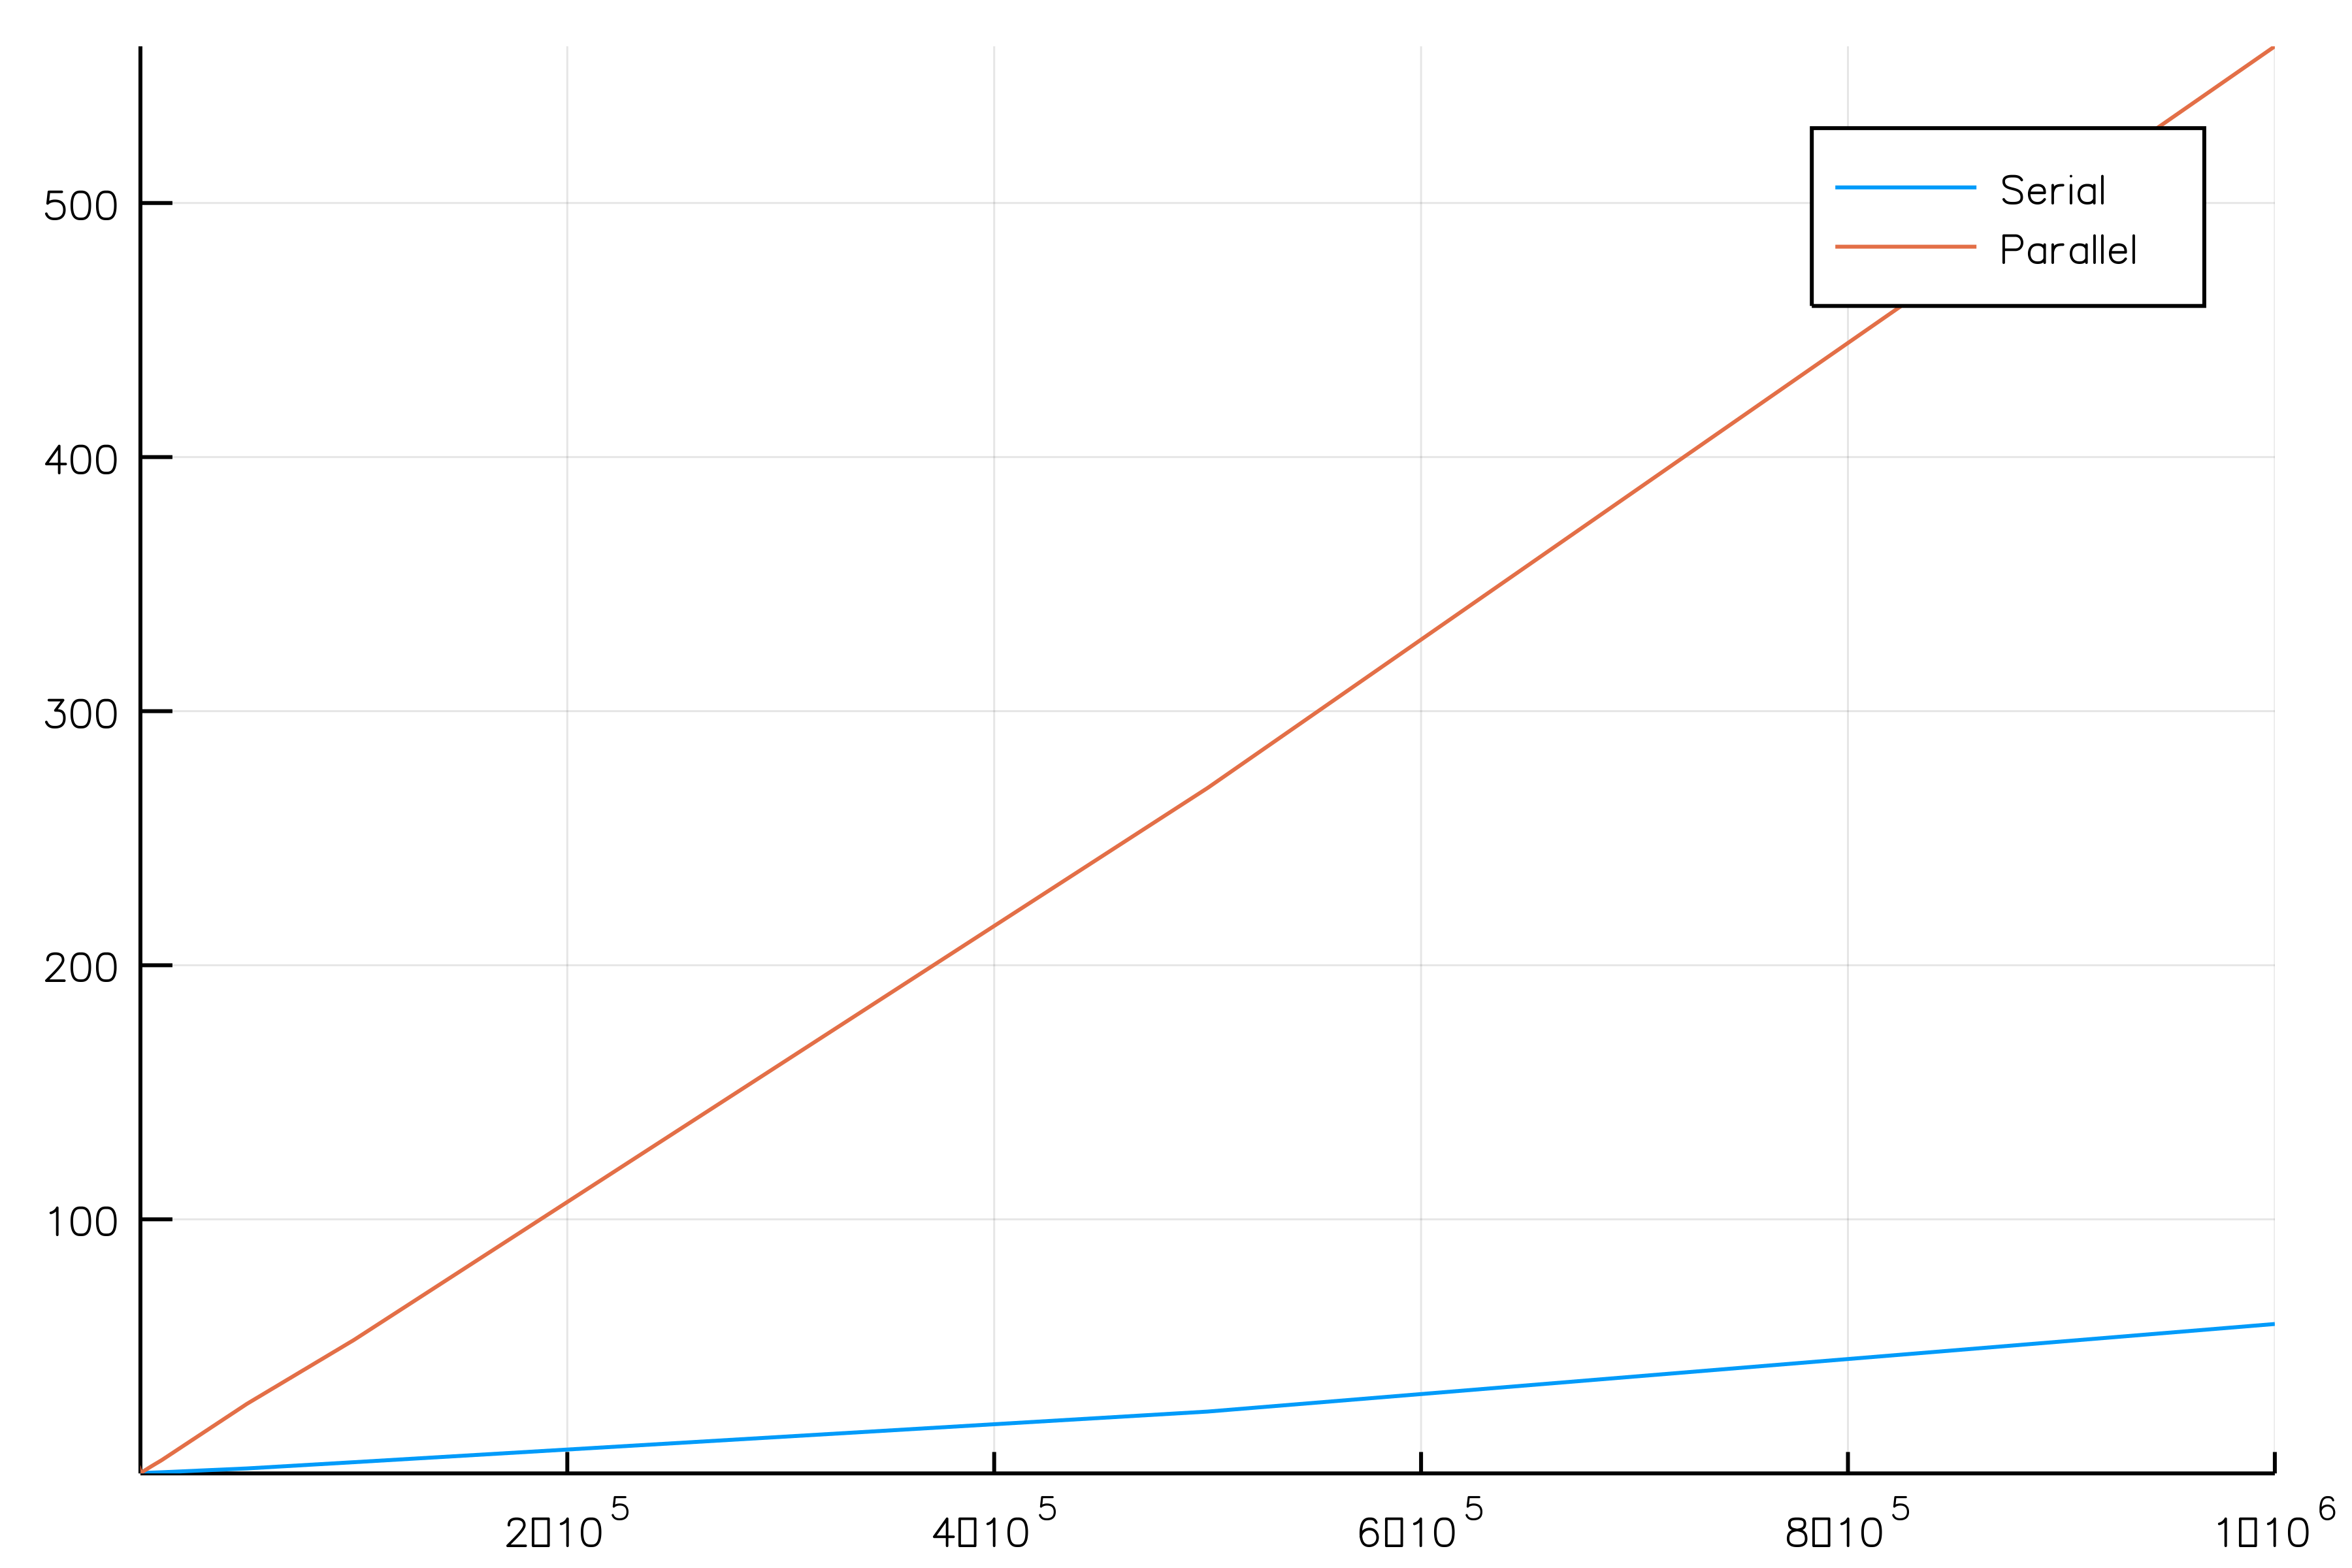
\includegraphics[scale=0.08]{compstruct2lar.png}
\caption{Compared execution time of function struct2lar on Tesla}
\end{figure}

%__________________________________________________________________________________________________________________________

\newpage
\subsection{larRemoveVertices}
\subsubsection{Conversion}

\noindent \framebox[5em][c]{\textbf{\normalsize Python}}
\begin{Verbatim}[fontsize=\scriptsize]

def larRemoveVertices(V,FV):
  vertDict = dict()
  index,defaultValue,FW,W = -1,-1,[],[]
  for k,incell in enumerate(FV):
    outcell = []
    for v in incell:
      key = vcode(4)(V[v])
      if vertDict.get(key,defaultValue) == defaultValue:
	index += 1
	vertDict[key] = index
	outcell += [index]
	W += [eval(key)]
      else:
	outcell += [vertDict[key]]
    FW += [outcell]
  return W,FW
  
\end{Verbatim}

\noindent \framebox[5em][c]{\textbf{\normalsize Julia}}
\begin{Verbatim}[fontsize=\scriptsize]

function larRemoveVertices(V,FV)
  vertDict= Dict()
  index,defaultValue,CW,W,FW = -1,-1,[],[],[]
  for (k,incell) in enumerate(FV)
    outcell=[]
    for v in incell
      key=vcode(4)(V[v+1])
      if get(vertDict,key,defaultValue)==defaultValue
	index =index+1
	vertDict[key]=index
	append!(outcell,index)
	append!(W,[eval(parse(key))])
      else
	append!(outcell,vertDict[key])
      end
    end
    append!(FW,[outcell])
  end
  return W,FW
end

\end{Verbatim}
\subsubsection{Parallelization}
\begin{Verbatim}[fontsize=\scriptsize]

@everywhere function plarRemoveVertices(V,FV)
  vertDict= Dict()
  index,defaultValue,CW,W,FW = -1,-1,[],[],[]
  @async begin
    for (k,incell) in enumerate(FV)
      outcell=[]
      @sync begin
	for v in incell
	  key=vcode(4)(V[v+1])
	  if get(vertDict,key,defaultValue)==defaultValue
	    index =index+1
	    vertDict[key]=index
	    append!(outcell,index)
	    append!(W,[eval(parse(key))])
	  else
	    append!(outcell,vertDict[key])
	  end
	end
      end
      append!(FW,[outcell])
    end
  end
  return W,FW
end

\end{Verbatim}

\subsubsection{Unit-Test}
\noindent\framebox[42em][c]{Serial Tests}
\begin{Verbatim}[fontsize=\footnotesize]

V=[[0,0,0],[0,0,1],[0,1,0],[0,1,1],[1,0,0],[1,0,1],[1, 1, 0], [1, 1, 1]]
FV=[[0,1,2,3],[4,5,6,7],[0,1,4,5],[2,3,6,7],[0,2,4,6],[1,3,5,7]]

@testset "larRemoveVertices Tests" begin
  @test typeof(larRemoveVertices(V,FV))==Tuple{Array{Any,1},Array{Any,1}}
  @test length(larRemoveVertices(V,FV)[1])<= length(V)
end

\end{Verbatim}
\framebox[42em][c]{Palallel Tests}
\begin{Verbatim}[fontsize=\footnotesize]
V=[[0,0,0],[0,0,1],[0,1,0],[0,1,1],[1,0,0],[1,0,1],[1, 1, 0], [1, 1, 1]]
FV=[[0,1,2,3],[4,5,6,7],[0,1,4,5],[2,3,6,7],[0,2,4,6],[1,3,5,7]]

@testset "plarRemoveVertices Tests" begin
  @test typeof(plarRemoveVertices(V,FV))==Tuple{Array{Any,1},Array{Any,1}}
  @test length(plarRemoveVertices(V,FV)[1])<= length(V)
end
\end{Verbatim}

\subsection{Result}
\textbf{Execution time on PC}
\begin{Verbatim}[fontsize=\footnotesize]
times=[]
ptimes=[]
append!(times,Time(larRemoveVertices,[l[i][1],l[i][2]]) for i in range(1,length(l)-1))
append!(ptimes,Time(plarRemoveVertices,[l[i][1],l[i][2]]) for i in range(1,length(l)-1))


plot(times,xlabel="input",xlims=(0,length(times)+2),ylabel="time(s)",label=["Serial"])
plot(ptimes,xlabel="input",xlims=(0,length(times)+2),ylabel="time(s)",label=["Parallel"])
\end{Verbatim}

\begin{figure*}[!h]
\centering
\subfloat[Serial]{%
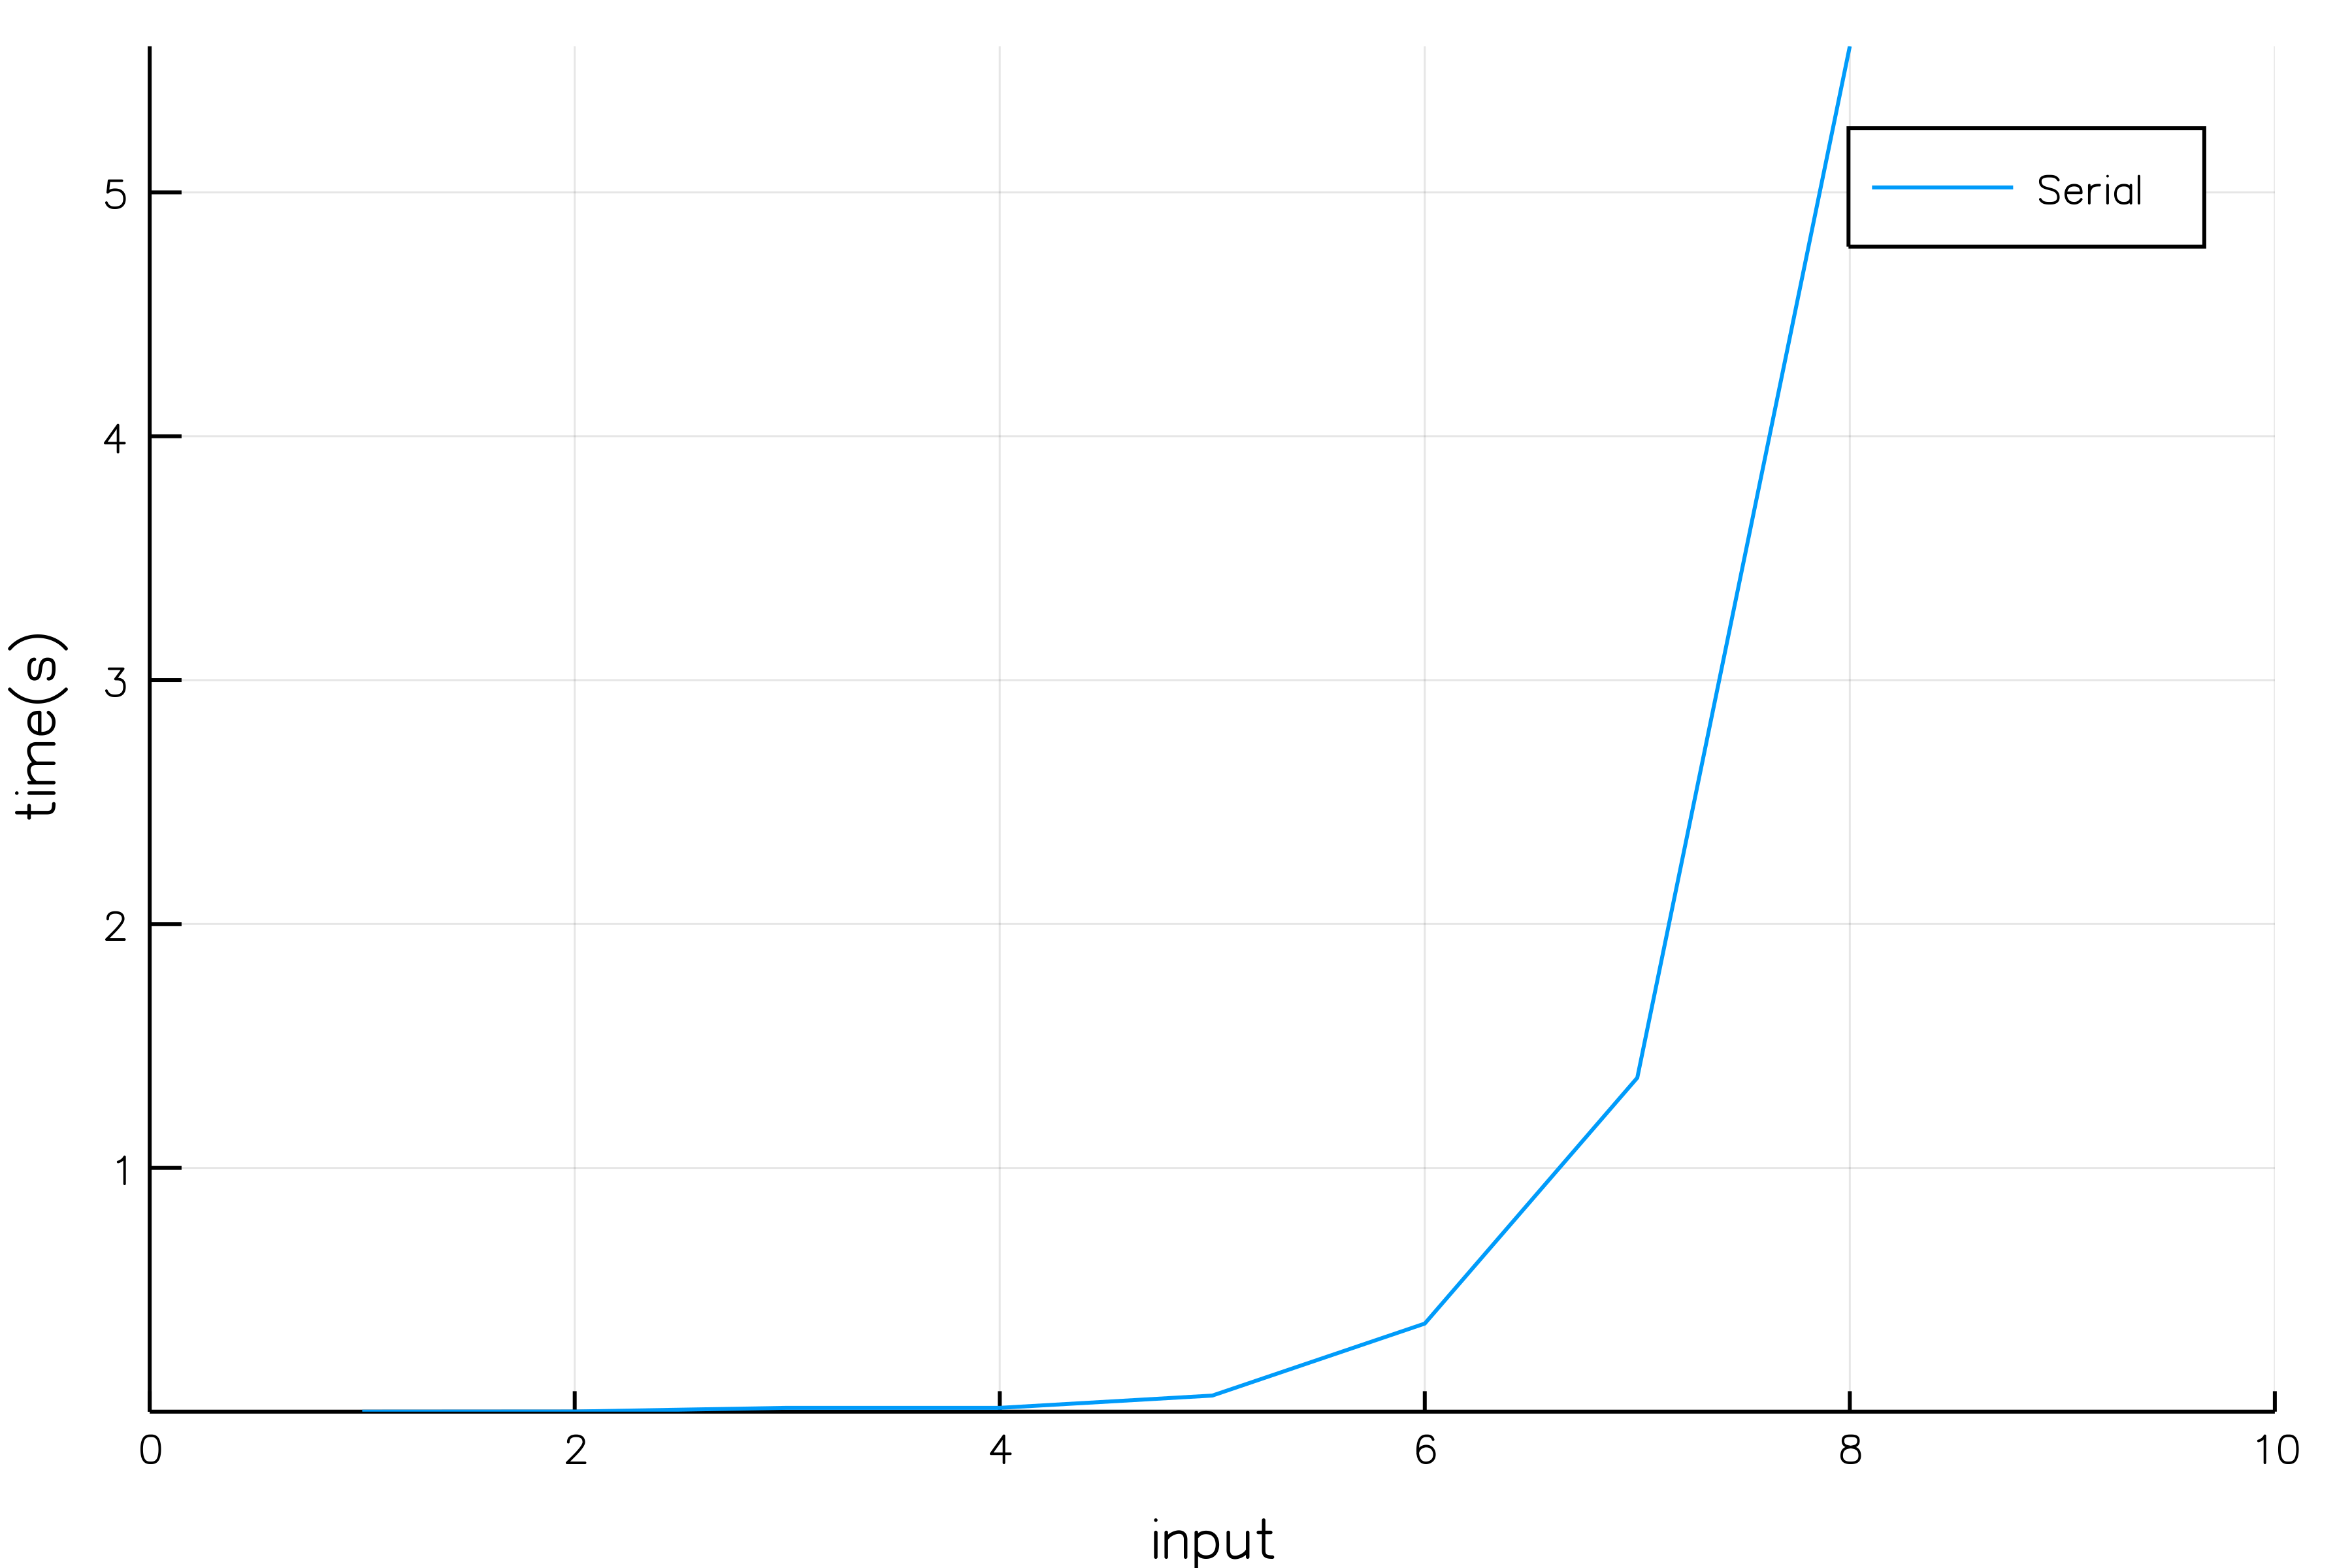
\includegraphics[scale=0.060]{larRemoveVertices.png}
}
\subfloat[Parallel]{%
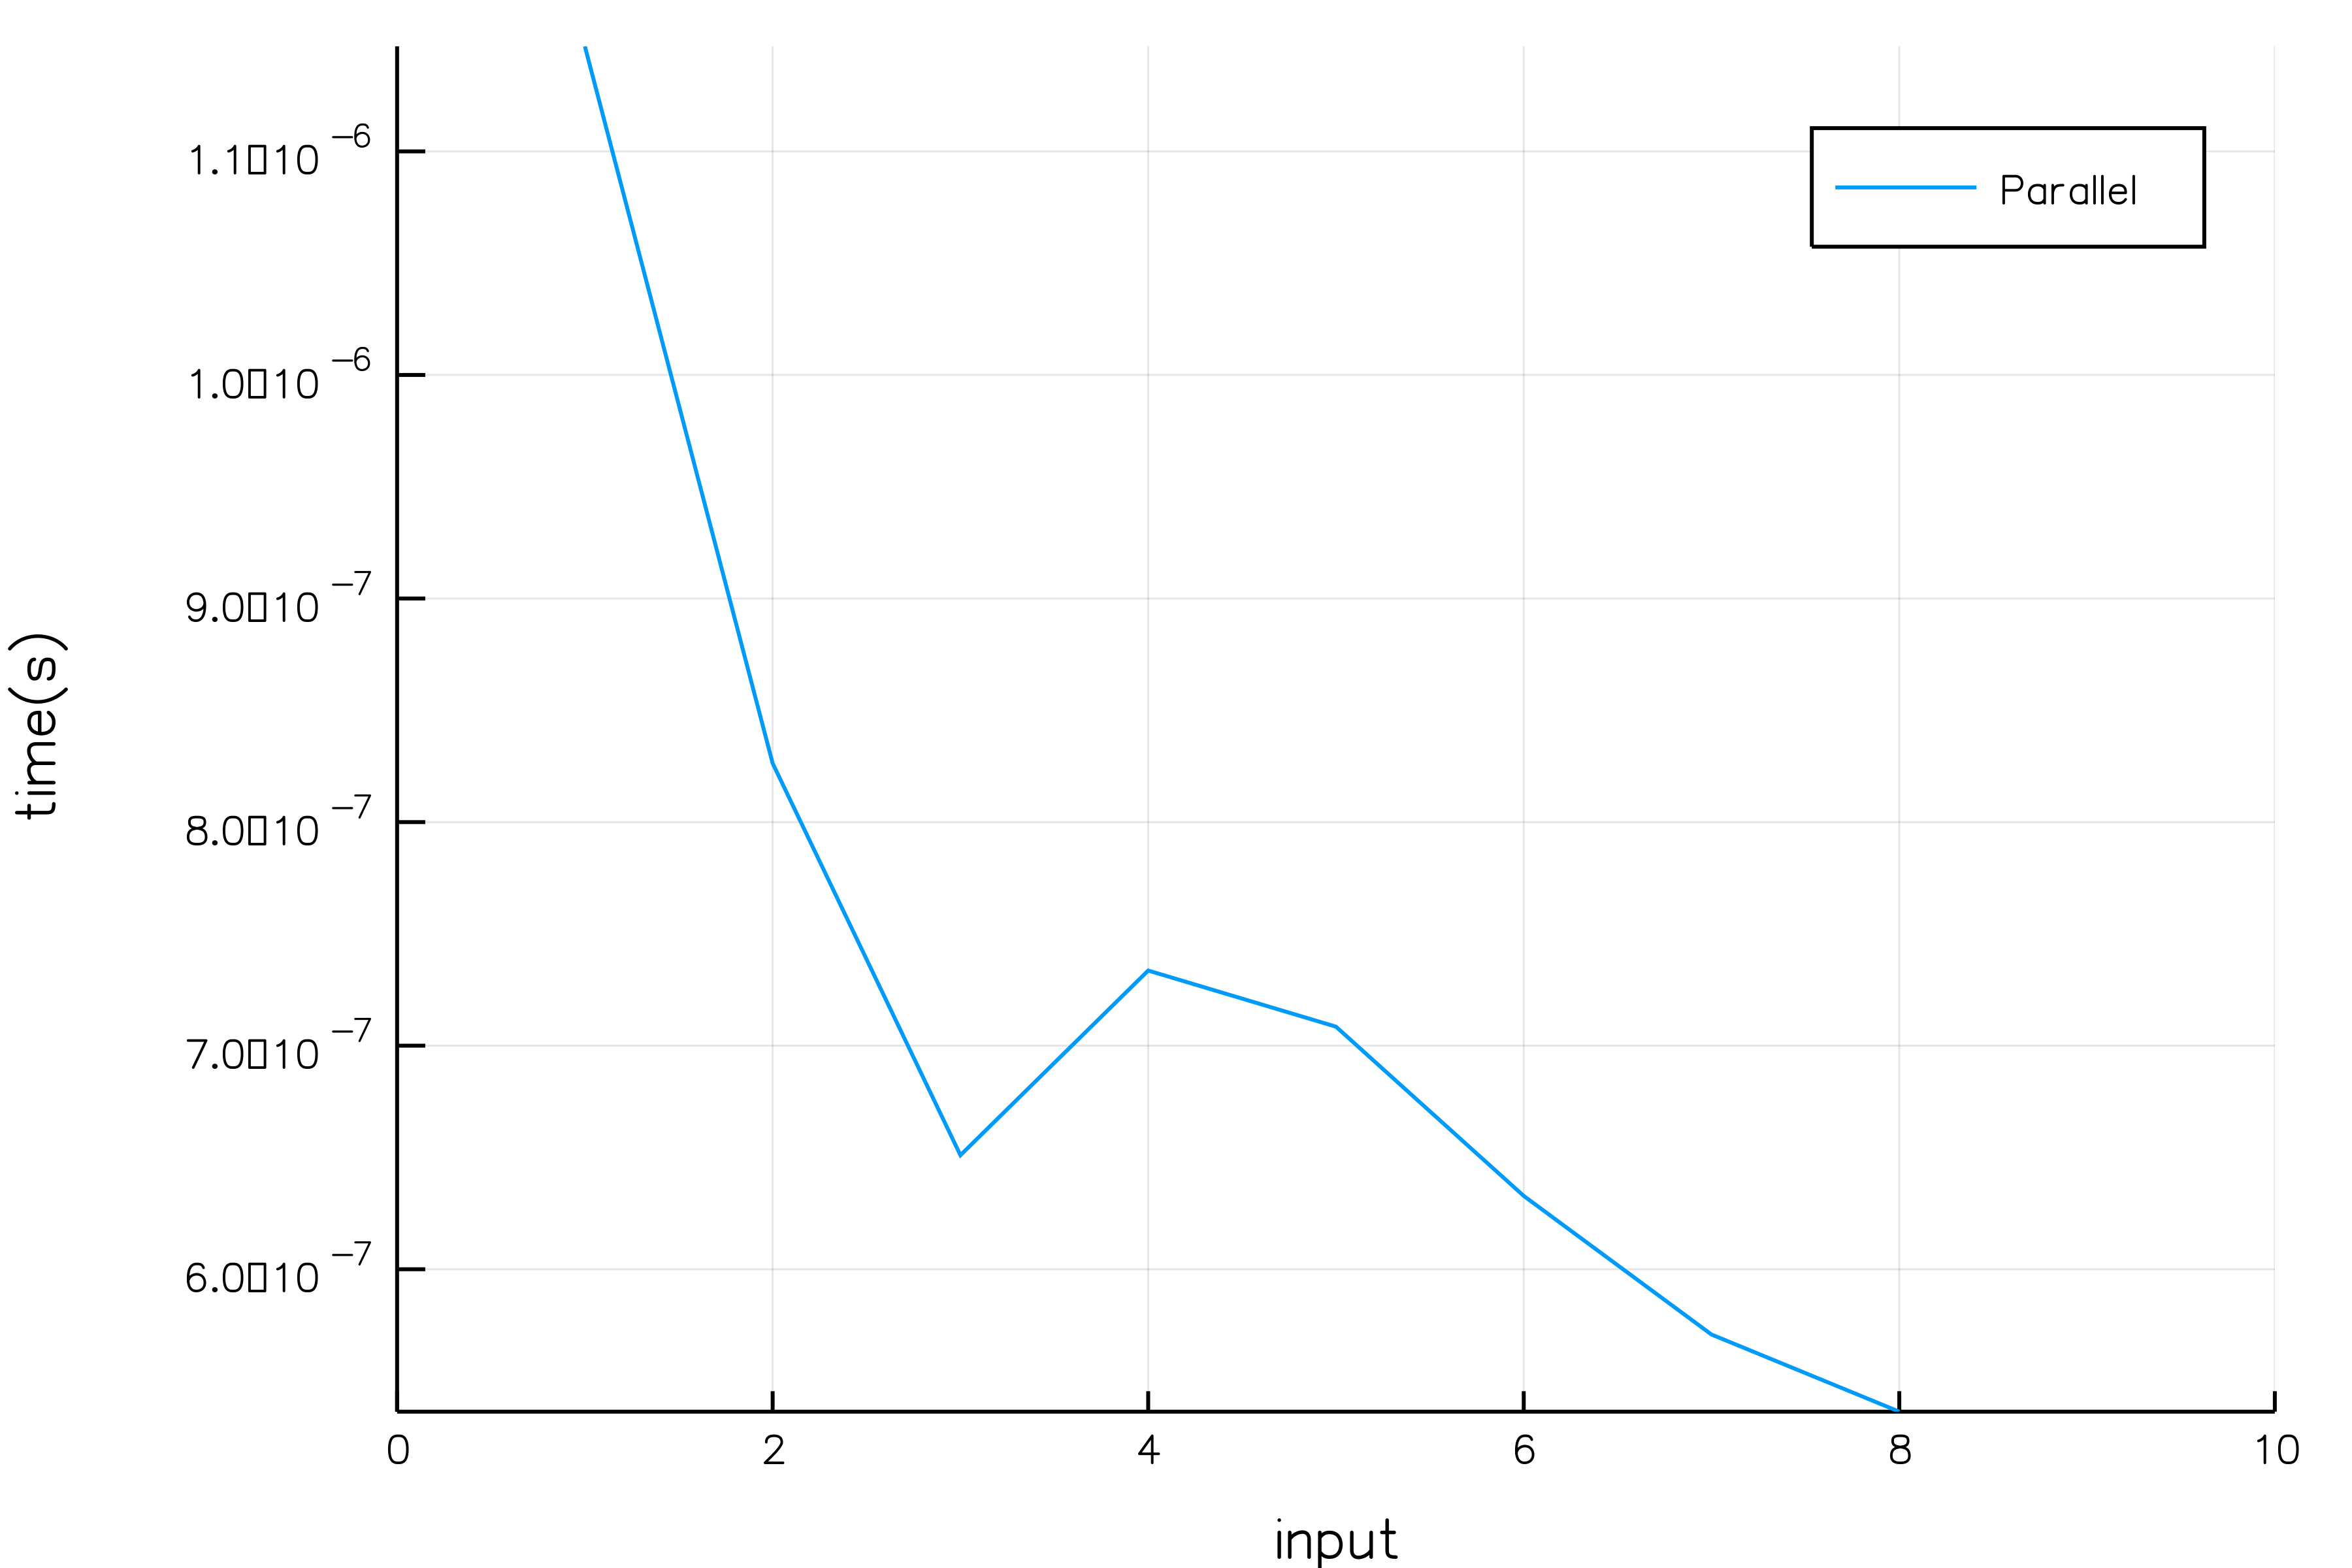
\includegraphics[scale=0.060]{larRemoveVerticesParallel.png}
}
\caption{Execution time of function larRemoveVertices}
\end{figure*}
\noindent \framebox[42em][c]{Compare}
\begin{Verbatim}[fontsize=\footnotesize]
plot([times,ptimes],xlabel="input",xlims=(0,length(times)+2),ylabel="time(s)",
label=["Serial","Parallel"])
\end{Verbatim}
\begin{figure}[!h]
\centering
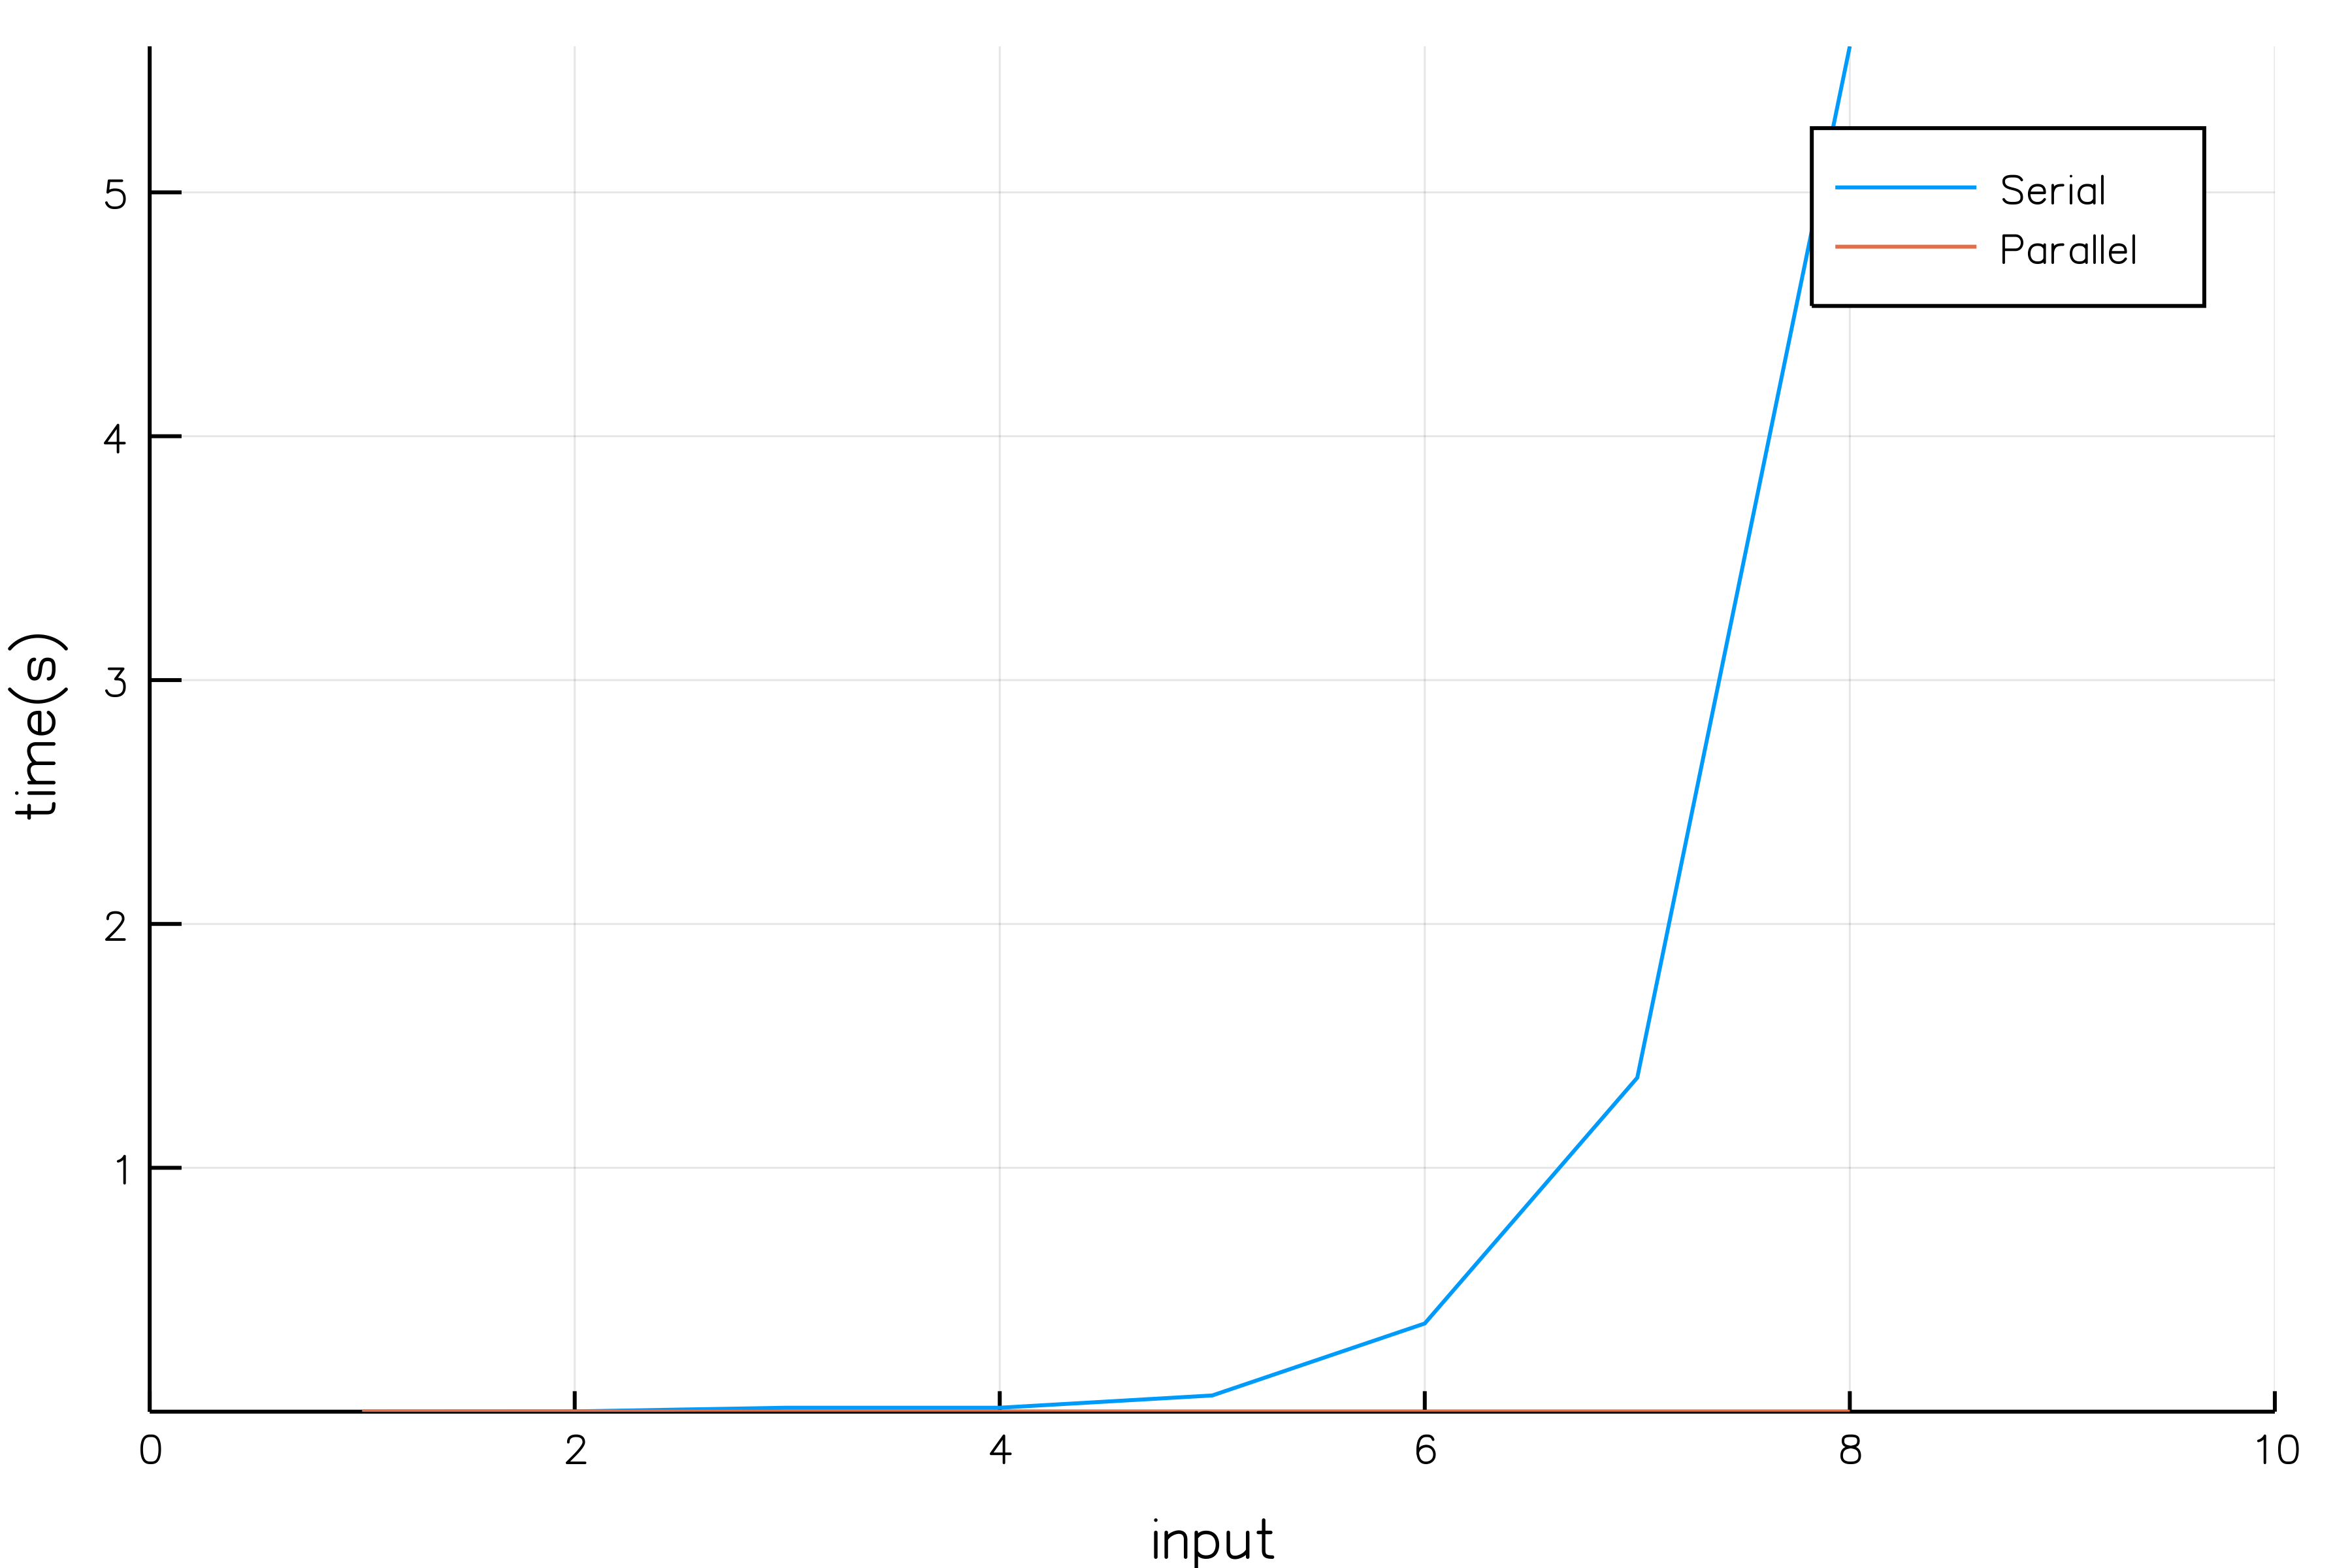
\includegraphics[scale=0.08]{larRemoveVerticesC.png}
\caption{Compared execution time of function larRemoveVertices}
\end{figure}

%__________________________________________________________________________________________________________________________
\newpage

\section{Examples}
In the following section some examples of how to use the module are presented.
\vspace{10px}

\noindent\textbf{Examples 1}
\begin{Verbatim}[fontsize=\footnotesize]
square= ([[0,0],[0,1],[1,0],[1,1]],[[0,1,2,3]])
table= larApply(t(-.5,-.5))(square)
chair= larApply(s(.35,.35))(table)
chair1= larApply(t(.75,0))(chair)
chair2= larApply(r(pi/2))(chair1)
chair3= larApply(r(pi/2))(chair2)
chair4= larApply(r(pi/2))(chair3)
\end{Verbatim}
This execution return the following immage:

\begin{figure}[!h]
\centering
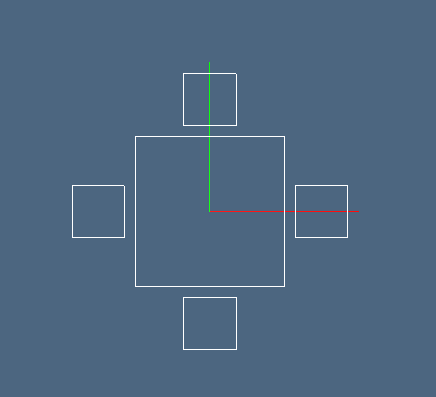
\includegraphics[scale=0.6]{tablewithchairs.png}
\caption{Table with four chair}
\end{figure}

\noindent\textbf{Examples 2}
\begin{Verbatim}[fontsize=\footnotesize]
desk=([[0, 0],[0, 1],[0, 2],[1, 0],[1, 1],[1, 2],[2, 0],[2, 1],[2, 2],[3, 0],[3, 1],[3, 2],
[4, 0],[4, 1],[4, 2],[5, 0],[5, 1],[5, 2],[6, 0],[6, 1],[6, 2],[7, 0],[7, 1],[7, 2],[8, 0],
[8, 1],[8, 2],[9, 0],[9, 1],[9, 2],[10, 0],[10, 1],[10, 2],[11, 0],[11, 1],[11, 2],[12, 0],
[12, 1],[12, 2],[13, 0],[13, 1],[13, 2],[14, 0],[14, 1],[14, 2],[15, 0],[15, 1],[15, 2],
[16, 0],[16, 1],[16, 2],[17, 0],[17, 1],[17, 2],[18, 0],[18, 1],[18, 2],[19, 0],[19, 1],
[19, 2],[20, 0],[20, 1],[20, 2]], [[0, 1, 3, 4],[1, 2, 4, 5],[3, 4, 6, 7],[4, 5, 7, 8],
[6, 7, 9, 10],[7, 8, 10, 11],[9, 10, 12, 13],[10, 11, 13, 14],[12, 13, 15, 16],
[13, 14, 16, 17],[15, 16, 18, 19],[16, 17, 19, 20],[18, 19, 21, 22],[19, 20, 22, 23],
[21, 22, 24, 25],[22, 23, 25, 26],[24, 25, 27, 28],[25, 26, 28, 29],[27, 28, 30, 31],
[28, 29, 31, 32],[30, 31, 33, 34],[31, 32, 34, 35],[33, 34, 36, 37],[34, 35, 37, 38],
[36, 37, 39, 40],[37, 38, 40, 41],[39, 40, 42, 43],[40, 41, 43, 44],[42, 43, 45, 46],
[43, 44, 46, 47],[45, 46, 48, 49],[46, 47, 49, 50],[48, 49, 51, 52],[49, 50, 52, 53],
[51, 52, 54, 55],[52, 53, 55, 56],[54, 55, 57, 58],[55, 56, 58, 59],[57, 58, 60, 61],
[58, 59, 61, 62]])
seat=larApply(s(0.02,0.3))(desk)
seat=larApply(t(0.55,-0.85))(seat)
line=Struct([desk,repeat([seat,t(1.65,0)],outer=12)...])
line=Struct([line,t(23,0),line])
lines=Struct([repeat([line,t(0,-3)],outer=6)...])
teacherdesk=larApply(s(0.5,0.8))(desk)
teacherdesk=larApply(t(16.5,5))(teacherdesk)
chair=larApply(s(0.15,0.5))(teacherdesk)
chair=larApply(t(18,5))(chair)
classroom=Struct([teacherdesk,chair,lines])
class=evalStruct(classroom)
\end{Verbatim}
This execution return the following immage:

\begin{figure}[!h]
\centering

\includegraphics[scale=0.6]{classroom.png}
\caption{Classroom}
\end{figure}

%__________________________________________________________________________________________________________________________
\newpage

\section{Conclusion}
It can be seen from the results of the graphs that parallelization generally slows down execution times. 
The execution times also depend on how the input is increased, in fact the execution times calculated on Tesla also increase for the sequential. 
Performing a parallelization on native language objects such as Tuple or Array is faster compared to one carried out on a Struct type object.

\addcontentsline{toc}{section}{References}
\begin{thebibliography}{9}
\bibitem{1} A.Paoluzzi
\href{https://github.com/cvdlab/lar-cc/blob/master/doc/pdf/larstruct.pdf}{Hierarchical structures with LAR},March 29,2016.
\bibitem{2} 
\href{https://docs.julialang.org/en/release-0.6/}{Julia Documentation}.
\end{thebibliography}
\end{document}
